\documentclass[12pt]{book}

\usepackage{natbib} % Tidies up citation numbers.
\usepackage[utf8]{inputenc}
\usepackage{graphicx}
\usepackage{pythonhighlight}
\usepackage{listingsutf8}
\usepackage{float}

%\def\UrlBreaks{\do\/\do-}
\usepackage[T1]{fontenc}
\usepackage{url}
\usepackage{breakurl}

\usepackage{pdfpages}

\lstset{
  extendedchars=true,
  language=java,
  basicstyle=\tiny\ttfamily,
  showspaces=false,
  showstringspaces=false,
    literate=
     {É}{{\'E}}{1}%
      {Á}{{\'A}}{1}%
      {Ã}{{\~A}}{1}%
      {Â}{{\^A}}{1}%
      {À}{{\`A}}{1}%
      {Ç}{{\,C}}{1}%
      {Ó}{{\'O}}{1}%
      {Í}{{\'I}}{1}%
      {Õ}{{\~O}}{1}%
      {Ú}{{\'U}}{1}%
      {ú}{{\'u}}{1}%
      {é}{{\'e}}{1}%
      {á}{{\'a}}{1}%
      {ã}{{\~a}}{1}%
      {à}{{\`a}}{1}%
      {â}{{\^a}}{1}%
      {ç}{{\,c}}{1}%
      {ó}{{\'o}}{1}%
      {í}{{\'i}}{1}%
      {õ}{{\~o}}{1}%
}

\definecolor{gray}{rgb}{0.4,0.4,0.4}
\definecolor{darkblue}{rgb}{0.0,0.0,0.6}
\definecolor{cyan}{rgb}{0.0,0.6,0.6}

\lstdefinelanguage{XML}
{
 numbers=left,
 numberstyle=\tiny,
 stepnumber=1,
 numbersep=8pt,
 morestring=[b]",
 morestring=[s]{>}{<},
 morecomment=[s]{<?}{?>},
 stringstyle=\color{black},
 identifierstyle=\color{darkblue},
 keywordstyle=\color{cyan},
 morekeywords={xmlns,version,type}% list your attributes here
}

\colorlet{punct}{red!60!black}
\definecolor{background}{HTML}{EEEEEE}
\definecolor{delim}{RGB}{20,105,176}
\colorlet{numb}{magenta!60!black}

\lstdefinelanguage{json}{
    basicstyle=\tiny\ttfamily,
    numbers=left,
    numberstyle=\tiny,
    stepnumber=1,
    numbersep=8pt,
    showstringspaces=false,
    breaklines=true,
    frame=lines,
    backgroundcolor=\color{background},
    literate=
     *{É}{{\'E}}{1}%
      {Á}{{\'A}}{1}%
      {Ã}{{\~A}}{1}%
      {Â}{{\^A}}{1}%
      {À}{{\`A}}{1}%
      {Ç}{{\,C}}{1}%
      {Ó}{{\'O}}{1}%
      {Í}{{\'I}}{1}%
      {Õ}{{\~O}}{1}%
      {Ú}{{\'U}}{1}%
      {ú}{{\'u}}{1}%
      {é}{{\'e}}{1}%
      {á}{{\'a}}{1}%
      {ã}{{\~a}}{1}%
      {à}{{\`a}}{1}%
      {â}{{\^a}}{1}%
      {ç}{{\,c}}{1}%
      {ó}{{\'o}}{1}%
      {í}{{\'i}}{1}%
      {õ}{{\~o}}{1}%
     {0}{{{\color{numb}0}}}{1}
      {1}{{{\color{numb}1}}}{1}
      {2}{{{\color{numb}2}}}{1}
      {3}{{{\color{numb}3}}}{1}
      {4}{{{\color{numb}4}}}{1}
      {5}{{{\color{numb}5}}}{1}
      {6}{{{\color{numb}6}}}{1}
      {7}{{{\color{numb}7}}}{1}
      {8}{{{\color{numb}8}}}{1}
      {9}{{{\color{numb}9}}}{1}
      {:}{{{\color{punct}{:}}}}{1}
      {,}{{{\color{punct}{,}}}}{1}
      {\{}{{{\color{delim}{\{}}}}{1}
      {\}}{{{\color{delim}{\}}}}}{1}
      {[}{{{\color{delim}{[}}}}{1}
      {]}{{{\color{delim}{]}}}}{1},
}

\lstdefinelanguage{SPARQL}{
    basicstyle=\tiny\ttfamily,
    numbers=left,
    numberstyle=\tiny,
    stepnumber=1,
    numbersep=8pt,
    showstringspaces=false,
    breaklines=true,
    frame=lines,
    backgroundcolor=\color{background},
    literate=
     {É}{{\'E}}{1}%
      {Á}{{\'A}}{1}%
      {Ã}{{\~A}}{1}%
      {Â}{{\^A}}{1}%
      {À}{{\`A}}{1}%
      {Ç}{{\,C}}{1}%
      {Ó}{{\'O}}{1}%
      {Í}{{\'I}}{1}%
      {Õ}{{\~O}}{1}%
      {Ú}{{\'U}}{1}%
      {ú}{{\'u}}{1}%
      {é}{{\'e}}{1}%
      {á}{{\'a}}{1}%
      {ã}{{\~a}}{1}%
      {à}{{\`a}}{1}%
      {â}{{\^a}}{1}%
      {ç}{{\,c}}{1}%
      {ó}{{\'o}}{1}%
      {í}{{\'i}}{1}%
      {õ}{{\~o}}{1},%
  morekeywords={
    SELECT,CONSTRUCT,DESCRIBE,ASK,WHERE,FROM,NAMED,PREFIX,BASE,OPTIONAL,
    FILTER,GRAPH,LIMIT,OFFSET,SERVICE,UNION,EXISTS,NOT,BINDINGS,MINUS,a
  }
}

\lstdefinelanguage{overpassQL}{
    basicstyle=\tiny\ttfamily,
    numbers=left,
    numberstyle=\tiny,
    stepnumber=1,
    numbersep=8pt,
    showstringspaces=false,
    breaklines=true,
    frame=lines,
    backgroundcolor=\color{background}
}

\lstset{language=R,
    literate=
    {<-}{{$\gets$}}1%
     {É}{{\'E}}{1}%
      {Á}{{\'A}}{1}%
      {Ã}{{\~A}}{1}%
      {Â}{{\^A}}{1}%
      {À}{{\`A}}{1}%
      {Ç}{{\,C}}{1}%
      {Ó}{{\'O}}{1}%
      {Í}{{\'I}}{1}%
      {Õ}{{\~O}}{1}%
      {Ú}{{\'U}}{1}%
      {ú}{{\'u}}{1}%
      {é}{{\'e}}{1}%
      {á}{{\'a}}{1}%
      {ã}{{\~a}}{1}%
      {à}{{\`a}}{1}%
      {â}{{\^a}}{1}%
      {ç}{{\,c}}{1}%
      {ó}{{\'o}}{1}%
      {í}{{\'i}}{1}%
      {õ}{{\~o}}{1},%
    basicstyle=\tiny\ttfamily,
    stringstyle=\color{red},
    otherkeywords={0,1,2,3,4,5,6,7,8,9},
    morekeywords={TRUE,FALSE},
    deletekeywords={data,frame,length,as,character},
    keywordstyle=\color{blue},
    commentstyle=\color{red},
}

\usepackage[brazil]{babel}  
\usepackage{xcolor}
%xcolor v2.12 (2016/05/11)384  Colors by Name4.1  Base colors (always available)black blue brown cyan darkgray gray green lightgray lime magenta olive orange pink purple red teal violet white yellow

\usepackage[nopostdot]{glossaries}
\setglossarystyle{altlist}
\PassOptionsToPackage{hyphens}{url}
\usepackage [colorlinks = true,
            linkcolor = blue,
            urlcolor  = blue,
            citecolor = blue,
            anchorcolor = blue]{hyperref} 

% gerador de lero-lero
\usepackage{lipsum}

\usepackage{pdfpages}

\newenvironment{itquote}
{\begin{quote}\itshape}
{\end{quote}}

\usepackage[commentmarkup=todo]{changes}

\usepackage{datetime2}

\usepackage{booktabs}

\usepackage{caption}
\input{packages-estudantes}

% define cores personalizadas para o texto de cada autor
\usepackage
%[final]
{changes}
%\usepackage{changes}
%\url{https://ctan.org/pkg/changes}

\definechangesauthor[name={Jorge Henrique Cabral Fernandes}, color=orange]{jhcf} % git-user: jhcf

\definechangesauthor[name={Alexsander Correa de Oliveira}, color=black]{KvotheKS} % git-user: KvotheKS OK

\definechangesauthor[name={Allann Gois Hoffmann}, color=orange]{AllannH} % git-user: AllannH OK

\definechangesauthor[name={André Larrosa Chimpliganond}, color=orange]{andrelarrosacrypt} % git-user: andrelarrosacrypt OK

\definechangesauthor[name={André Cássio Barros de Souza}, color=green]{andreloff} % git-user: andreloff OK

\definechangesauthor[name={Bruno Sanguinetti Regadas de Barros}, color=blue]{Jaxiii} % git-user: Jaxiii OK

\definechangesauthor[name={Enzo Nunes Leal Sampaio}, color=orange]{enzodevs2000} % git-user: enzodevs2000 OK

\definechangesauthor[name={Felipe Gomes Paradas}, color=pink]{fparadas} % git-user: fparadas OK

\definechangesauthor[name={Lucas de Almeida Bandeira Macedo}, color=teal]{ABMHub} % git-user: ABMHub OK

\definechangesauthor[name={Fernanda Macedo de Sousa}, color=magenta]{fernandams} % git-user: fernandams Ok

\definechangesauthor[name={Gabriel dos Santos Martins}, color=green]{gsmartins96} %  git-user: gsmartins96 OK

\definechangesauthor[name={Gabriel Faustino Lima da Rocha}, color=gray]{Faustino27} %  git-user: Faustino27 OK

\definechangesauthor[name={Gabriel Martins de Almeida}, color=purple]{GMalme} %  git-user: GMalme OK

\definechangesauthor[name={Gabriel Rocha Fontenele}, color=pink]{ngsylar} % git-user: ngsylar OK

\definechangesauthor[name={Ítalo Eduardo Dias Frota}, color=pink]{titofrota} % git-user: titofrota OK

\definechangesauthor[name={João Antonio Desidério de Moraes}, color=teal]{joaoadm94} % git-user: joaoadm94 OK

\definechangesauthor[name={Ualiton Ventura da Silva}, color=orange]{uventura} % git-user: uventura OK

\definechangesauthor[name={Pedro de Torres Maschio}, color=orange]{pedro-maschio} % git-user: pedro-maschio OK

\definechangesauthor[name={Tong Zhou}, color=orange]{Tong00020} % git-user: Tong00020 Ok

\definechangesauthor[name={Gustavo Rodrigues dos Santos}, color=pink]{gutorsantos} % git-user: gutorsantos OK

\definechangesauthor[name={Gustavo Tomás de Paula}, color=green]{gustavo-tomas} % git-user: gustavo-tomas OK

\definechangesauthor[name={Gustavo Macedo de Carvalho}, color=purple]{GustavoMacCar} % git-user: GustavoMacCar OK

\definechangesauthor[name={Arthur da Silveira Couto}, color=purple]{CrimsonCrown} % git-user: CrimsonCrown OK?

\definechangesauthor[name={Vitor de Oliveira Araujo Araruna}, color=orange]{vitorararuna} % git-user: vitorararuna OK

\definechangesauthor[name={Rafael dos Santos Silva}, color=red]{rafaelsilva21} % git-user: rafaelsilva21 OK

\definechangesauthor[name={Marcus Vinicius Oliveira de Abrantes}, color=red]{MarcusABR} % git-user: MarcusABR OK

\definechangesauthor[name={Mateus de Paula Rodrigues}, color=cyan]{MoustacheGolem} % git-user: MoustacheGolem OK

\definechangesauthor[name={Leonardo Alves Riether}, color=blue]{LeoRiether} % git-user: LeoRiether OK

\definechangesauthor[name={Tatiana Franco Pereira}, color=cyan]{Tatianafp} % git-user: Tatianafp OK

\definechangesauthor[name={Vinícius Caixeta de Souza}, color=orange]{vinis-caixe} % git-user: vinis-caixe OK

\definechangesauthor[name={Conrado Nunes Barbosa Neto}, color=blue]{Conras21} % git-user: Conras21 OK

\definechangesauthor[name={Stefano Luppi Sposito}, color=pink]{KawaiiStheno} % git-user: KawaiiStheno OK

\definechangesauthor[name={João Pedro Felix de Almeida}, color=teal]{DYosplay} % git-user: DYosplay OK

\definechangesauthor[name={João Víctor Siqueira de Araujo}, color=red]{StrawHat972} % git-user: StrawHat972 OK

\definechangesauthor[name={Raylan da Silva Sales}, color=pink]{Rayxan} % git-user: Rayxan OK

\definechangesauthor[name={Guilherme Oliveira Loiola}, color=blue]{guioliunb} % git-user: guioliunb OK

\definechangesauthor[name={Paulo Alvim Alvarenga}, color=purple]{alvimpaulo} % git-user: alvimpaulo OK

\definechangesauthor[name={Léo Akira Abe Barros}, color=red]{leoakir} % git-user: leoakir OK

\definechangesauthor[name={Enzo Yoshio Niho}, color=purple]{enzoyoshio} % git-user: enzoyoshio OK

\definechangesauthor[name={Daniel Rodrigues Cardoso}, color=blue]{DanielrCardoso} % git-user: DanielrCardoso OK

\definechangesauthor[name={Fernando Ferreira Cordeiro}, color=blue]{FernandoCordeiro} % git-user: FernandoCordeiro OK

\definechangesauthor[name={Jônatas Gomes Barbosa da Silva}, color=cyan]{jonatas1n} % git-user: jonatas1n OK

\definechangesauthor[name={Lucas Gabriel de Oliveira Gurgel Fernandes}, color=black]{lggurgel} % git-user: lggurgel OK

\definechangesauthor[name={Bruno Esteves Dalla Costa Filho}, color=red]{brunoedcf} % git-user: brunoedcf OK

\definechangesauthor[name={Paulo Mauricio Costa Lopes}, color=red]{RequiemDosVivos} % git-user: RequiemDosVivos OK

\definechangesauthor[name ={Caio Bernardon Nascif Kaawi Massucato}, color=blue]{CaioMassucato} % git-user: CaioMassucato OK 

\makenoidxglossaries
\loadglsentries{1-Introducao/tarefas/1.1-Glossario/estudantes/main}

\setcounter{tocdepth}{5}
\setcounter{secnumdepth}{5}
\captionsetup[table]{name=Quadro}
\renewcommand{\lstlistingname}{Listagem de Código}

\newcommand{\dataset}{\textit{dataset}}
\newcommand{\query}{\textit{query}}
\newcommand{\githubusername}{\textless githubusername\textgreater}

\begin{document}
\pagenumbering{gobble}% Remove page numbers (and reset to 1)
\clearpage
\thispagestyle{empty}

\begin{titlepage}
\begin{center}
 {\huge\bfseries 
\includegraphics[width=4cm]{unb-logo.jpg}\\
	CIC0203 - Computação Experimental - TA - 2021.2\\\url{https://www.overleaf.com/project/618e9b4b0db7234d6d9fbfc0}\\
	Notas e Registros\\}
 % ----------------------------------------------------------------
 \vspace{1.5cm}
{\large	% author names and affiliations
	Jorge Henrique Cabral Fernandes}\\
	André Larrosa Chimpliganond\\
	Alexsander Correa de Oliveira\\
	Allann Gois Hoffmann\\
	André Cássio Barros de Souza\\
	Arthur da Silveira Couto\\
	Bruno Esteves Dalla Costa Filho\\
	Bruno Sanguinetti Regadas de Barros\\
	Caio Bernardon Nascif Kaawi Massucato\\
	Conrado Nunes Barbosa Neto\\
	Daniel Rodrigues Cardoso\\
	Enzo Nunes Leal Sampaio\\
	Enzo Yoshio Niho\\
	Fernanda Macedo de Sousa \\
	Fernando Ferreira Cordeiro \\
	Felipe Gomes Paradas\\
	Gabriel dos Santos Martins\\
	Gabriel Faustino Lima da Rocha\\
	Gabriel Martins de Almeida\\
	Gabriel Rocha Fontenele\\
	Gustavo Macedo de Carvalho\\
	Gustavo Rodrigues dos Santos \\
	Gustavo Tomás de Paula\\
	Ítalo Eduardo Dias Frota\\
	João Pedro Felix de Almeida\\
	João Víctor Siqueira de Araujo\\
	Jônatas Gomes Barbosa da Silva\\
	Léo Akira Abe Barros\\
	Leonardo Alves Riether\\
	Lucas de Almeida Bandeira Macedo\\
	Lucas Gabriel de Oliveira Gurgel Fernandes \\
	Mateus de Paula Rodrigues\\
	Marcus Vinicius Oliveira de Abrantes\\
	Paulo Mauricio Costa Lopes\\
	Pedro de Torres Maschio\\
	Rafael dos Santos Silva\\
	Rafael Henrique Nogalha de Lima\\
	Raylan da Silva Sales\\
	Stefano Luppi Spósito\\
	Tatiana Franco Pereira\\
	Tong Zhou\\
	Ualiton Ventura da Silva\\
	Vinícius Caixeta de Souza\\
	Guilherme Oliveira Loiola\\
	Artur Filgueiras Scheiba Zorron\\
	Vitor de Oliveira Araujo Araruna \\
	\vspace{1.5cm}
	{\large Brasília, \DTMnow}
\end{center}
\end{titlepage}
	%\date{10 de março de 2021}
	% make the title area
%	\maketitle
    \listoftodos
	\printnoidxglossary
	\tableofcontents
	\listoffigures
	\listoftables
	\clearpage
\pagenumbering{arabic}

\pagestyle{fancy}

	\chapter*{Resumo}

	Este documento contém notas de aula e registros em geral, produzidos de forma textual, pelo professor e turma da disciplina CIC0203 - Computação Experimental - TA - 2021.2.
	
	A disciplina adotará a abordagem de estudos estatísticos de simulações computacionais, como base para a construção de experimentos.

\chapter{Orientações Iniciais}

Leia atentamente as orientações a seguir, tendo em vista que lhe auxiliarão no melhor desempenho neste curso-disciplina. 

\section{Importância deste documento}

Este documento contém o registro de todas as evidências de aprendizagem suas, e dos demais estudantes que fazem parte do curso Computação Experimental.
Quando for editar este documento tome cuidado para sempre deixá-lo em plena condição compilável, e sem erros. Busque também resolver os \textit{warnings} causados pelas suas edições.

Todos os pacotes de trabalho que você depositar deverão ser acessíveis, de forma direta ou indireta, a partir do arquivo ``main.tex'', no diretório raiz.

\section{Uso sincronizado de Repositório no Github.com e Overleaf.com}

Todo o código deste documento está na plataforma Overleaf.com, mantido sincronizado como o repositório CE-20212 na plataforma Github.com, disponível na url \url{https://github.com/jhcf/Comput-Experim-20212}, que é o repositório \textbf{origin}.

Dessa forma, para poder realizar a disciplina todos os estudantes devem ter uma conta pessoal em github.com, bem como uma conta pessoal em overleaf.com. Inicie registrando o seu nome completo e \textbf{github username} no arquivo autores.tex, onde você também deve escolher uma cor para uso no registro de alterações, conforme disponível no pacote ``changes''.

O acesso de gravação no Repositório ser-lhe-á concedido pelo professor do curso ao final da primeira semana de aula.

\section{Depósito dos pacotes de trabalho referentes à execução das tarefas}

A execução de toda e qualquer tarefa pontuável neste curso é feita por meio do depósito de um pacote de trabalho no repositório, contendo textos, programas de computador e outros dados coletados e (ou) analisados. Todos os textos e códigos no repositório devem estar em formato não compactado. Apenas os arquivos de dados muito grandes devem ser compactados em formato zip. Não usar rar, gz etc. 

Todo pacote de trabalho a ser avaliado precisa estar integralmente armazenado no Repositório CE-20212 / origin (e consequentemente sincronizável com o Overleaf).

\subsection{Onde depositar os pacotes de trabalho?}

Toda e qualquer inserção de texto, programa de computador, dados, enfim, qualquer documento, feito por estudante, deve ocorrer em um dos seguintes pontos:
\begin{enumerate}
    \item Dentro de um subdiretório com o código da tarefa, no diretório de ``experiments'' do estudante, onde o nome do diretório de \texttt{experiments} de um estudante é o seu github username (veja, por exemplo, o professor, que tem como github username: jhcf);
    \item Dentro dos diretórios ``tarefas'', nos diretórios dos temas de estudo;
    \item No arquivo ``autores.tex'';
    \item No arquivo ``packages-estudantes.tex'', onde eventualmente podem ser inseridos novos pacotes para apoiar o uso de algum recurso específico; e
    \item Na substituição do arquivo RESIC.bib por outro mais recente, obtido pela exportação completa da biblioteca RESIC que se encontra na plataforma Zotero, na url \url{https://www.zotero.org/groups/2465026/resic}.
\end{enumerate}

Não serão avaliados os pacotes de trabalhos entregues em local distinto do especificado, ou não acessíveis por meio do output em PDF, resultante da compilação de ``main.tex''.

\section{Entrega das tarefas}

Toda pontuação concedida ao/à estudante será feita mediante:
\begin{enumerate}
    \item Sincronização plena entre o documento no Overleaf.com e o repositório no Github.com;
    \item O registro de execução da correspondente tarefa no ambiente Moodle do curso, feita pelo estudante até o limite de prazo informado;
\end{enumerate}

Se a tarefa é feita em grupo, cada um dos membros do grupo deve obrigatoriamente fazer o registro da execução da tarefa, com as mesmas informações. Os membros do grupo devem evitar qualquer duplicação de código e textos no Overleaf. Ou seja, depositar os pacotes de trabalho referentes a cada tarefa em apenas um dos diretórios de experimentos de um dos membros do grupo. Até o final do curso, todos os membros de um grupo devem aparecer como produtores de pelo menos um pacote de trabalho feito pelo grupo.

\section{Escrevendo o texto}

Cuidados ao escrever texto:
\begin{description}
\item [Reconhecimento de autorias] Faça citações a textos e ideias que não são de sua autoria, usando referências registradas no grupo Zotero RESIC. Sempre informe os nomes completos dos autores dos relatórios, logo após o título do relatório;
\item [Grafia] A boa ortografia e gramática são essenciais à valorização de um trabalho. Descuido com essa questão revela, de forma geral, descuido e (ou) desinteresse pelo próprio trabalho, influenciando a pontuação obtida;
\item [Referências a códigos e dados] Toda e qualquer de escrita de relatório deverá fazer referência explícita ao diretório no Repositório, onde se encontram os códigos e dados usados para produção do relatório. No ambiente Moodle não será aceita a entrega de arquivos compactados contendo os resultados de realização das tarefas;
\end{description}

\section{Organização do ambiente experimental}

A organização do ambiente experimental de cada estudante é essencial para a realização adequada das tarefas.
Alguns dos problemas típicos que refletem descuido com a organização do trabalho de laboratório, são:

\begin{enumerate}
\item Problemas com merge durante operação no repositório git;
\item Uso inadequado de caracteres com acentuação nos nomes dos arquivos;
\item Não informar os ponteiros adequados, seja por meio das tags \LaTeX~ input e (ou) includepdf, de modo que a tarefa fica inacessível e invisível na tabela de conteúdos gerada a partir da compilação do documento main.tex.
\end{enumerate}

\subsection{Problemas com merge durante operações de push no Git}

Cada estudante é inteiramente responsável por fazer os merges manuais para entrega de sua tarefa no Repositório, caso o branch correspondente ao seu pacote de trabalho não consiga ser feito de forma automática. 

Estudantes que deixarem merges em conflito, prejudicando o processo de envio dos trabalhos dos demais, poderão perder pontos pela não entrega do trabalho no prazo, bem como pelo conflito causado para os demais estudantes do curso-disciplina. 

Busque informações sobre como resolver merges no livro Pro Git \cite{chacon_pro_2014}, ou em  urls como \url{https://www.zotero.org/groups/2465026/resic/collections/C7BG9S2W/items/HCY5X8PT/note/9M2BFISL/collection}

\subsection{Uso inadequado de nomes para arquivos}

Devido ao fato de que estaremos trabalhando em um ambiente laboratorial compartilhado, com uso de muitas linguagens combinadas, como \LaTeX, Python e R, entre outras, é fundamental adotar um padrão de nomeação para arquivos e diretórios. Atualmente esse padrão é composto pelas seguintes regras:
\begin{enumerate}
    \item Não use caracteres de acentuação em nomes de arquivos;
    \item Não use espaço em branco em nomes de arquivos;
    \item Não use underline em nomes de arquivos. Usar hífen em vez de Underline;
    \item Para nomes de arquivos longos use a \url{https://pt.wikipedia.org/wiki/CamelCase}, e eventualmente misture com o uso de hifens, para melhor legibilidade.
\end{enumerate}

\subsection{Não colocar os ponteiros adequados para que a tarefa seja visível}

É necessário que todo trabalho a ser avaliado esteja visível a partir da tabela de conteúdos gerada pela compilação do documento main.tex, sejam em um capítulo, seção ou subseção em \LaTeX.



\part{Introdução\label{part:intro}}

    \chapter{Aula/Texto de Apoio: O que é a Ciência?}

    
Existem várias definições sobre o que é a ciência. Algumas questões sobre essa definição são apresentadas por \citep{fernandes_consideracoes_2021}, cujo texto está reproduzido a seguir. 

A figura \ref{fig:ciencia-filosofia}~ apresenta um mapa conceitual que trata da fundamentação do conceito de ciência e sua relação com a filosofia.
Veja o vídeo da aula de 20 de janeiro de 2022, para mais detalhes.

\begin{figure}
    \centering
    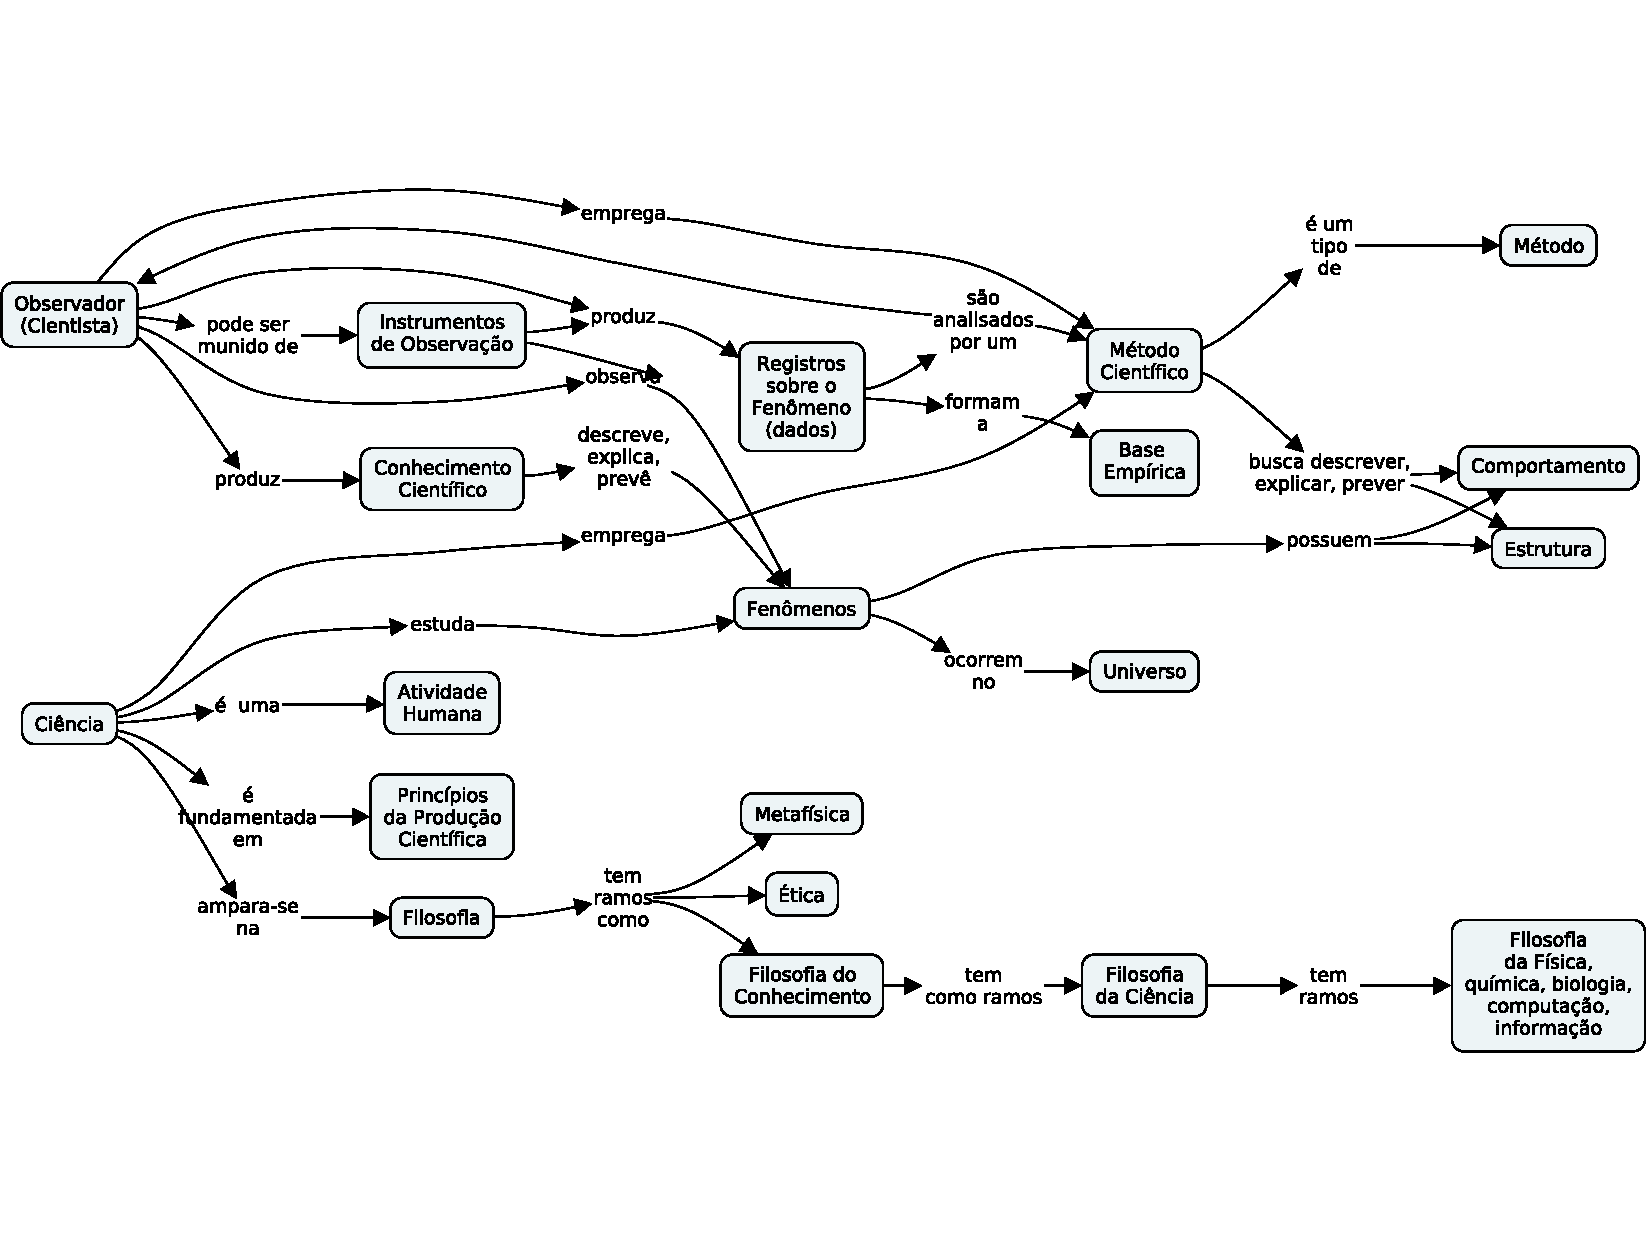
\includegraphics[page=1,angle=90,width=1\textwidth]{1-Introducao/aulas/Ciencia-e-Filosofia.pdf}
    \caption{Conceitos fundamentais de ciência, e sua relação com a filosofia. Fonte: jhcf}
    \label{fig:ciencia-filosofia}
\end{figure}

A figura \ref{fig:desenv-sw-ciencia-filosofia} acrescenta à figura  \ref{fig:ciencia-filosofia}~ os conceitos que relacionam a natureza do desenvolvimento de software à  fundamentação do conceito de ciência e sua relação com a filosofia.
Veja o vídeo  da aula de 20 de janeiro de 2022, para mais detalhes.

\begin{figure}
    \centering
    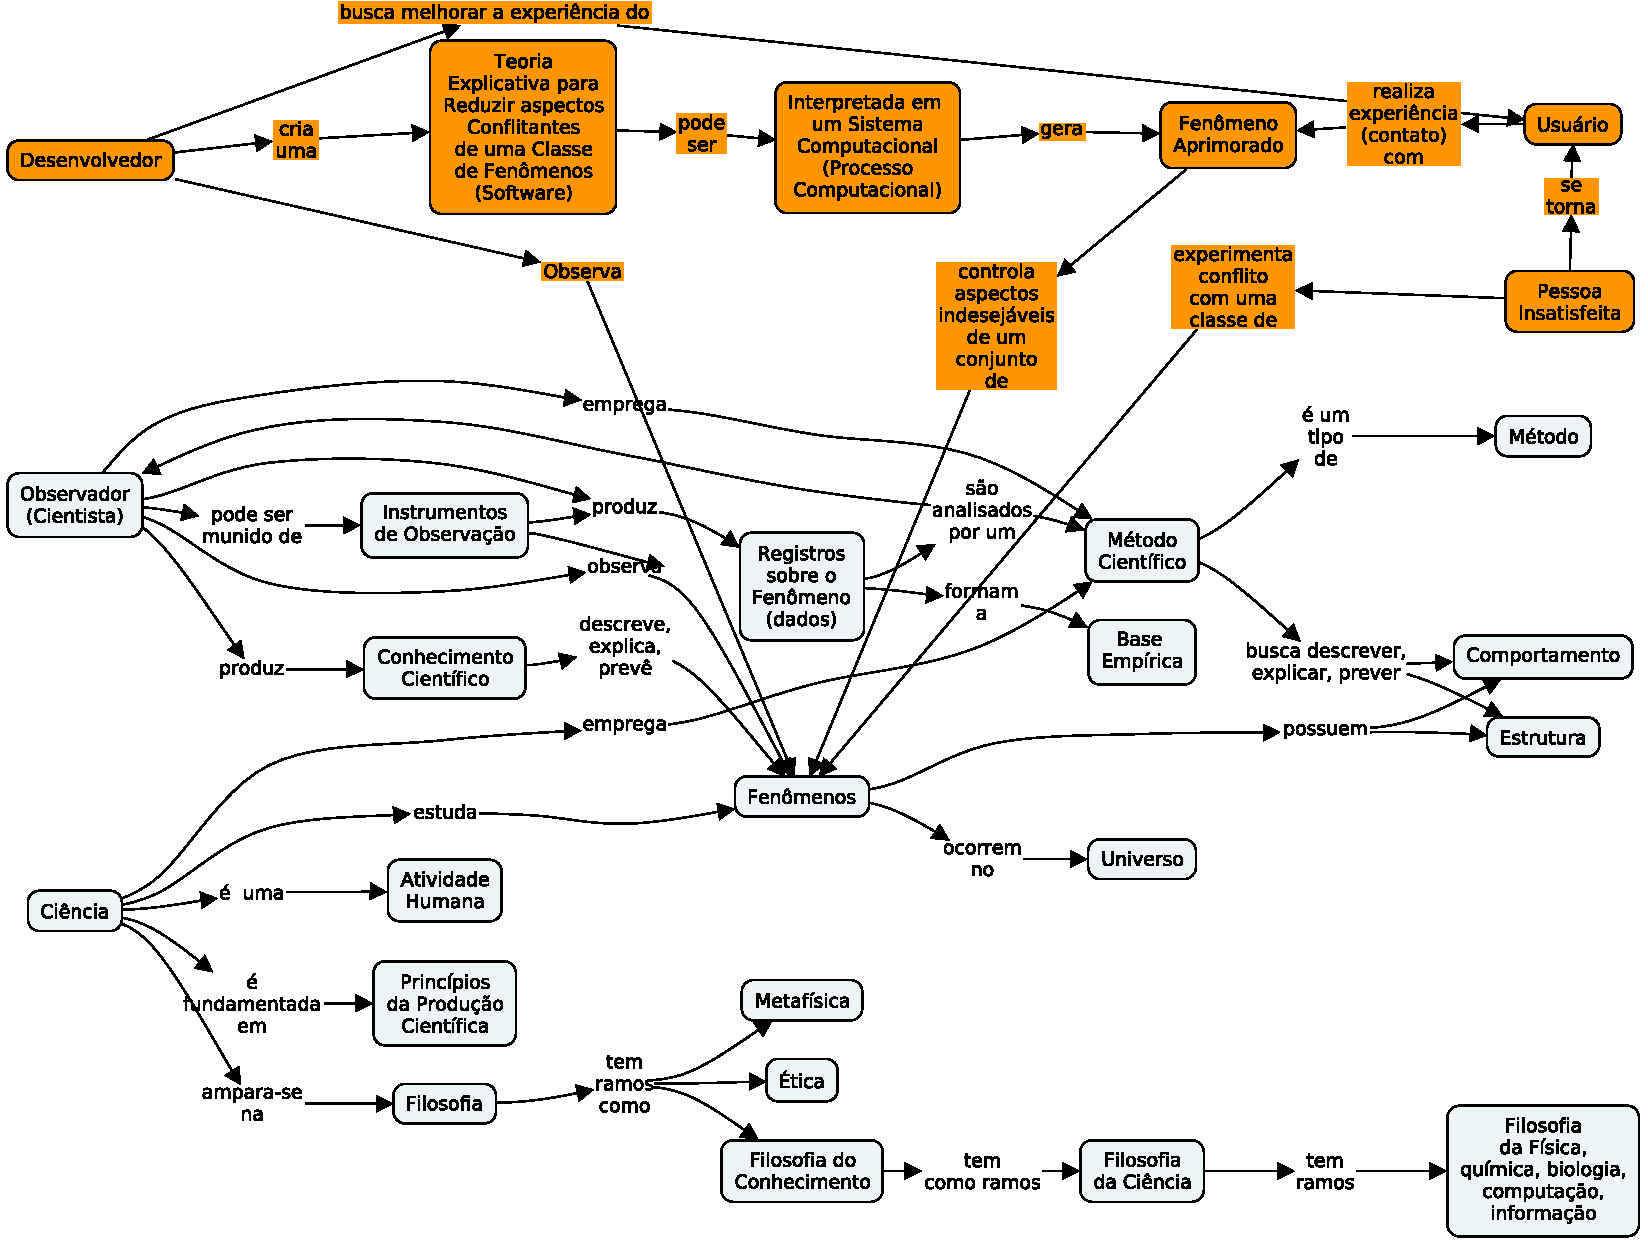
\includegraphics[page=1,angle=90,width=1\textwidth]{1-Introducao/aulas/Desenvolvimento-de-Software-Ciencia-e-Filosofia.pdf}
    \caption{Como a atividade do desenvolvimento de software se compara à atividade cientifica? Fonte: jhcf}
    \label{fig:desenv-sw-ciencia-filosofia}
\end{figure}

A figura \ref{fig:principios:ativ:cientifica}~ sumariza, em um mapa conceitual, os princípios da atividade científica e os relaciona com os princípios do desenvolvimento de software.
Veja o vídeo da aula de 20 de janeiro de 2022, para mais detalhes.

\begin{figure}
    \centering
    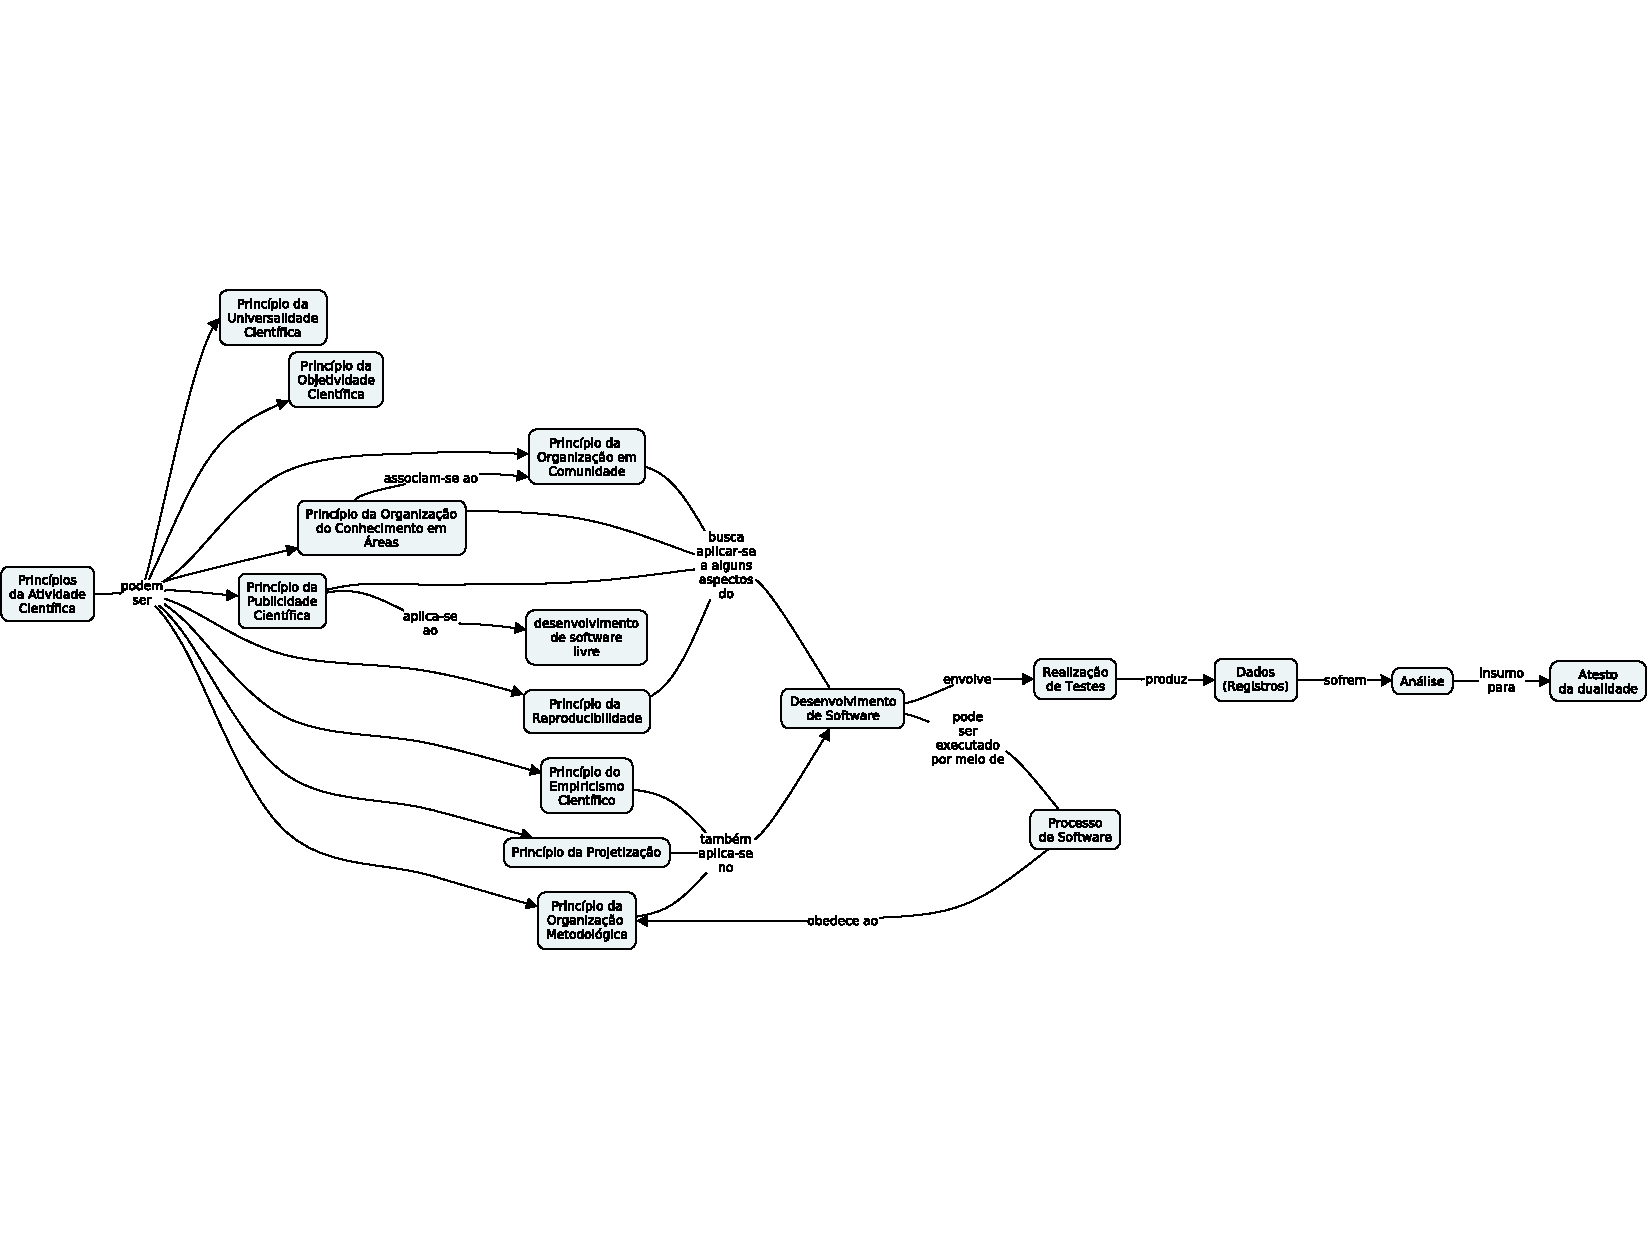
\includegraphics[page=1,angle=90,width=1\textwidth]{1-Introducao/aulas/Principios-da-atividade-cientifica.pdf}
    \caption{Quais os princípios da  atividade cientifica? como se relacionam com a atividade de desenvolvimento de software. Fonte: jhcf}
    \label{fig:principios:ativ:cientifica}
\end{figure}

A ciência positivista não pode ser feita sem uso de \gls{Dado}.
\gls{Derek Solla Price} é conhecido como o pai da  cientometria.


	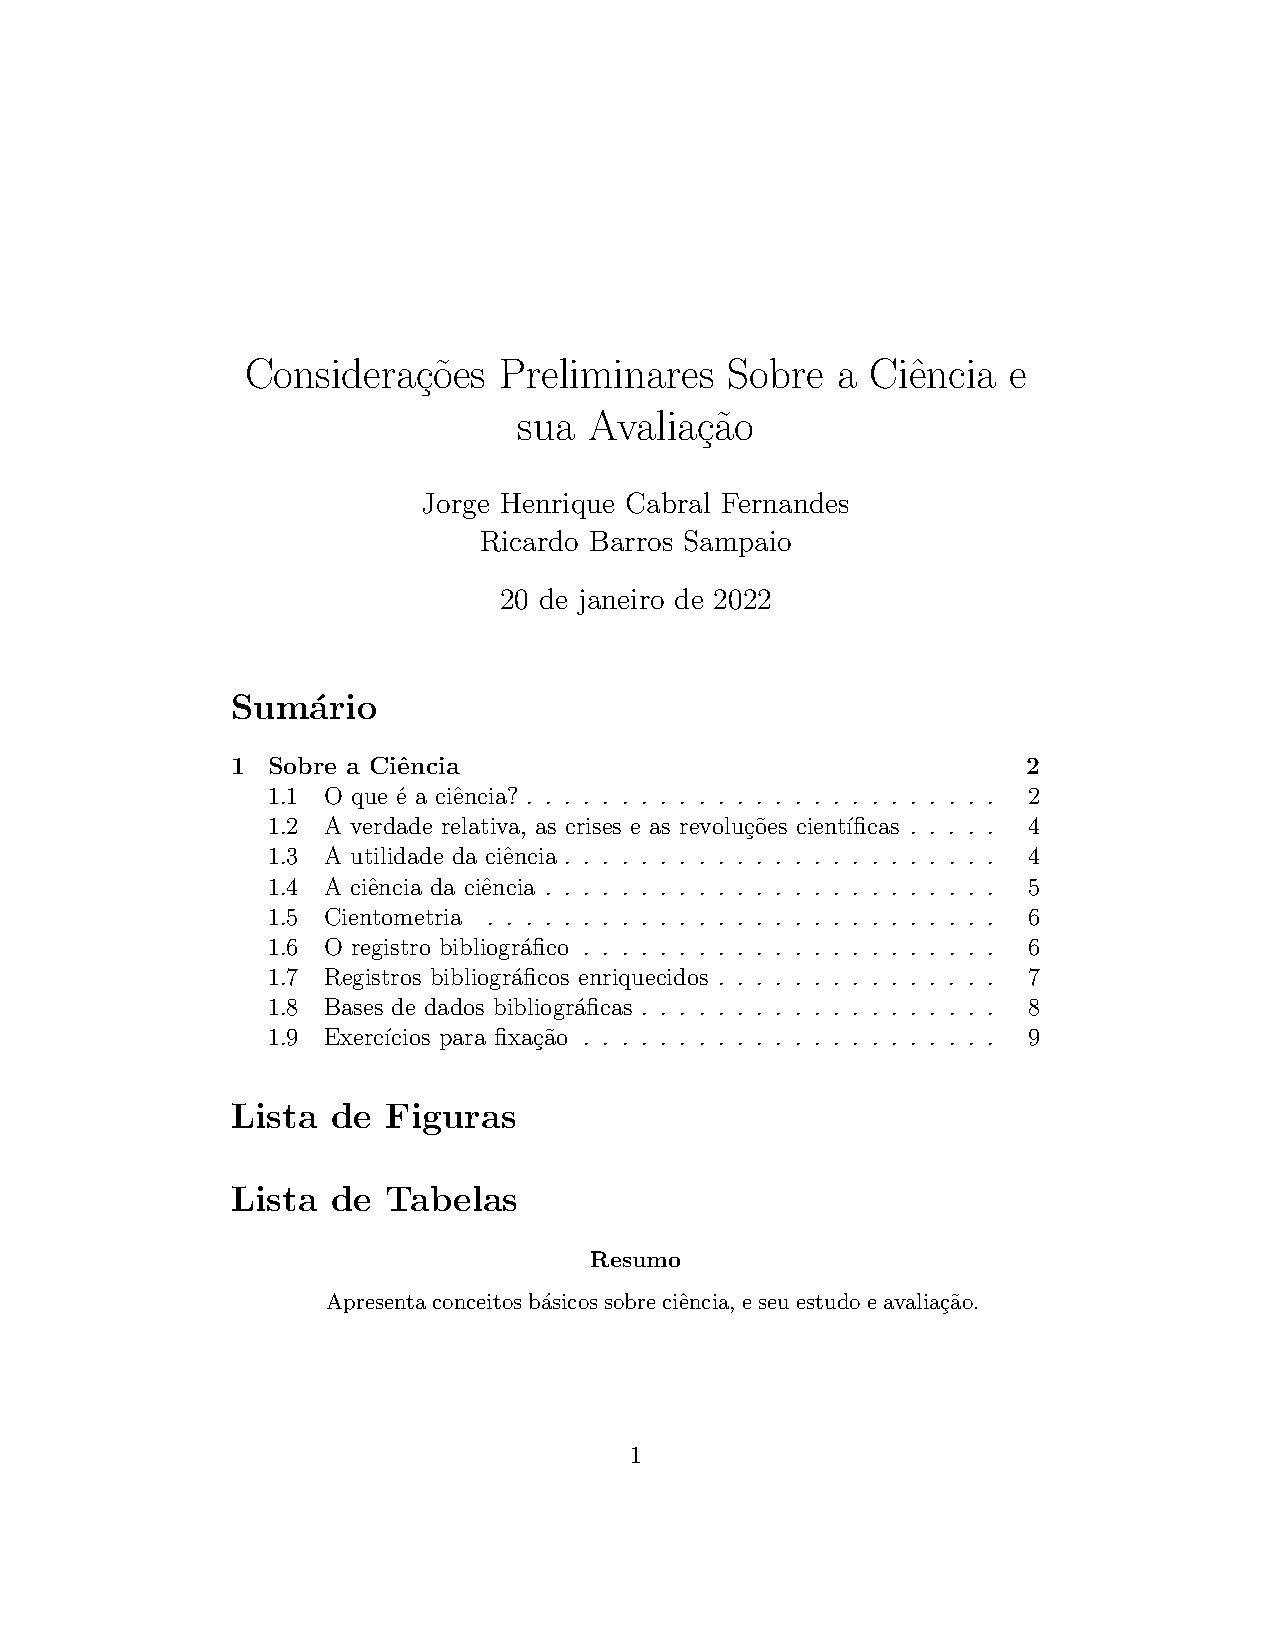
\includepdf[pages=-]{1-Introducao/aulas/Ciencia-e-sua-Avaliacao} %o link permite que isso possa ser citado - DYosplay


    \chapter{Tarefas: Glossário e impressões Iniciais Sobre a Ciência}
    
    \section{Tarefa: Criar um item no glossário deste documento \label{tarefa:glossario}}

Registre, no glossário do relatório da disciplina, uma definição de um termo relacionado com o texto de considerações preliminares sobre a ciência, de autoria do professor, em para ``1-Introducao/aulas/Consideracoes-Preliminares-Sobre-a-Ciencia-e-sua-Avaliacao.pdf''.

O diretório onde o arquivo deve ser criado é: 
1-Introducao/tarefas/1.1-Glossario/estudantes

O nome do arquivo á ser criado por você deve ter a forma:
tarefa-\githubusername.tex, e deve seguir o modelo da tarefa exemplo do professor, em
1-Introducao/tarefas/1.1-Glossario/estudantes/tarefa-jhcf.tex

O texto do item de glossário que você vai criar deve ser escrito em língua portuguesa, e conter uma definição para o termo e um exemplo de caso concreto.

A definição deve referenciar pelo menos um item bibliográfico presente no grupo Zotero.

A sua resposta a essa atividade vale até 3\% da pontuação total da disciplina.
Veja como exemplo a resposta do professor, na primeira seção.


 
    \section{Tarefa 3: Registrar suas impressões iniciais sobre a ciência, citando pelo menos  um item no glossário}

\gls{Comunidade Científica}

Cada estudante, a partir do que já sabe e leu, deve criar no diretório a seguir uma seção com o seu nome, a fim de apresentar um ou dois parágrafos de sua autoria, apresentando as suas \textbf{Impressões iniciais sobre o que é a Ciência}: 

O diretório onde o arquivo deve ser criado é: 
1-Introducao/tarefas/1.2-Impressoes-Ciencia/estudantes

O nome do arquivo á ser criado deve ter a forma:
tarefa-\githubusername.tex, e deve seguir o modelo da tarefa exemplo do professor, em
1-Introducao/tarefas/1.2-Impressoes-Ciencia/estudantes/tarefa-jhcf.tex

No registro de suas impressões iniciais no texto da tarefa, você precisa:
\begin{itemize}
    \item Usar um ou mais dos itens do glossário, incluído o que você criou na tarefa \ref{tarefa:glossario};
    \item Usar uma ou mais citações a referências bibliográficas usando a tag \verb|\citet{}| ou \verb|\citep{}|. Não use a tag \verb|\url{}|. Note que todas as referências citadas devem estar registradas no arquivo RESIC.bib, gerado a partir da bibliografia no grupo RESIC em \url{https://www.zotero.org/groups/2465026/resic}, ao qual você deve ter acesso, como feito em tarefa anterior.
\end{itemize}

A sua resposta a essa atividade vale até 3\% da pontuação total da disciplina.
Veja como exemplo a resposta do professor, na primeira seção.

\subsection{Minhas impressões iniciais sobre a ciência, por Jorge Henrique Cabral Fernandes}

A ciência da computação \citep{baldwin_three-fold_1994}, uma ciência específica dentre as várias existentes, apresenta-se muito relacionada com a filosofia da ciência \citep{floridi_blackwell_2004}, ou como uma meta-ciência (A filosofia é um campo do pensamento humano que é base para a ciência). Um exemplo que comprova essa versatilidade - ou até mesmo universalidade - da Ciência da Computação é o emprego da computação, sendo como exemplo mais concreto o uso de simulação, como método de pesquisa empírica, isso é pesquisa baseada em coleta e análise de dados \cite{marcolino_a_2014,tedre_experiments_2014}. A versatilidade do computador, decorrente do software, inclusive de simulação, gera uma plataforma empírica - o computador é prodigioso na coleta, cálculo e geração de dado - para o desenho e execução de quase todo tipo de experimento científico em quaisquer dos outros campos do conhecimento. Situações mais específicas podem ser vistas no campo da \gls{EA}.


\subsection{Minhas impressões iniciais sobre a ciência, por Stefano Luppi Sposito}

Desde o início na humanidade, o ser humano possui um desejo insaciável pelo conhecimento. A busca por algo novo sempre possuiu um papel extremamente importante ao longo da evolução humana. Atualmente, definimos \gls{Ciencia} como o tipo de conhecimento que busca verdades para compreender o funcionamento das coisas \citep{gnipper_o_nodate}.

As verdades buscadas podem ser encontradas através da \gls{Experimentacao} de diversas teorias para que evidências sejam conseguidas, a fim de comprovar que teorias e pensamentos estão corretos. É possível afirmar com certeza absoluta que experimentos são uma parte fundamental na parte da ciência que tanto nos ajuda, pois através deles, a própria ciência pode ser executada, levando o homem à lua ou à menor partícula existente. \citep{rabelo_o_2011}

\subsection{Minhas impressões iniciais sobre a ciência, por Tong Zhou}

A ciência \gls{RC}

\newglossaryentry{Derek Solla Price}{
	name={Derek Solla Price},
	description={'Derek John de Solla Price (22 de janeiro de 1922 — 3 de setembro de 1983) foi um físico, historiador da ciência e cientista da informação, conhecido principalmente como o pai da cienciometria. Price é também lembrado por cunhar a expressão "grande ciência" (big science).' Fonte: \citet{wikipedia_derek_2018}
	}
}

\subsection{Minhas impressões iniciais sobre a ciência, por Gustavo Tomás de Paula}

O positivismo \citep{wikipedia_positivismo_2022} é uma corrente filosófica que defende que o conhecimento verdadeiro é derivado pela razão e lógica por meio de experiências sensoriais. No texto "Considerações Preliminares Sobre a Ciência e sua Avaliação", é possível notar essa influência, nos tópicos que se referem, principalmente, ao empiricismo e projetização da ciência. Esses métodos são amplamente utilizados na computação, no momento em que o desenvolvimento de algoritmos que simulam o comportamento de órbitas de corpos celestiais, por exemplo, é derivado da astrofísica e suas áreas correlatas, que fazem forte uso da observação e de resultados empíricos \gls{Positivismo}.


\subsection{Minhas impressões iniciais sobre a ciência, por Gabriel Rocha Fontenele}

A \gls{Ciencia} ampara-se fundamentalmente na filosofia como base para servir o propósito de descrever, explicar ou prever \gls{fenomeno}s do universo \citep{floridi_blackwell_2004}. Tal filosofia abrange a sub-área da Filosofia da Ciência, que estuda aspectos mais subjetivos da ciência ao tentar responder perguntas como "o que é o cientista?", "como os fenômenos devem ser observados?" ou "como deve se estruturar um método para produzir conhecimento científico?".

Tais perguntas concebem conceitos e definições que a ciência se apropria para estudar os fenômenos de forma objetiva -, com perguntas sobre como se manifestam, quais o fatores desencadeadores, o que provocam e explicações sobre os resultados obtidos. Para isso, a ciência faz uso do \gls{EmpirismoCientifico}: os dados coletados produzirão informações relevantes e possíveis soluções para um dado problema inserido no contexto do fenômeno.

\subsection{Minhas impressões iniciais sobre a ciência, por Alexsander Correa de Oliveira}

A ciência da computação, enquanto ciência, é uma das áreas mais subestimadas, pois computação sempre toma a frente, tanto em fundos, quanto em visibilidade. Isso tudo é apenas uma falta de conhecimento sobre como ela é estruturada, pois é sem dúvida uma das ciências mais diferentes. A aplicação de grandes \emph{break-troughs} é quase imediata, como pode ser observado em algoritmos como busca binária e as buscas em grafos criadas por Dijkstra. 
Além do mais, os problemas computacionais tendem a ser mais facilmente apresentáveis para um publico \emph{pop} \citep{wikipedia_scientific_2021}, como um exemplo podemos apresentar um dos problemas do milênio, $P = NP$, em que existem claras aplicações em jogos como xadrez. Essa facilidade de compreensão superficial, muita das vezes, acaba por gerar também o efeito já citado, o de subestimarem a real força da ciência da computação enquanto meio intelectual. 


\subsection{Minhas impressões iniciais sobre a ciência, por Enzo Nunes Leal Sampaio}


A ciência é algo difícil de definir, pois não existe um conceito único e aceito por todos sobre sua definição, segundo \citet{schwartzman_ciencia_1984}. Contudo, a sua importância para o ser humano durante toda a sua história é inegável. Ela permitiu vários avanços para a humanidade como por exemplo: aumento da expectativa de vida, aumento da produtividade de fábricas, a globalização, etc. Infelizmente, na atualidade, vários grupos anti-ciência têm duvidado dos méritos dela como mostra o artigo dos pesquisadores \citet{scherma_relatos_2020}.

Diante disso, o conhecimento sobre o método científico é crucial para que os cientistas possam tentar mostrar como a ciência é feita e que ela segue vários princípios pré-estabelecidos. Um desses princípios é o da Publicidade Científica e este princípio afirma a importância da documentação da atividade científica e é nesse ponto que o uso de ferramentas como o \gls{Bibtex} ajudam nesse processo para criar, por exemplo, os documentos via LaTex, no qual, os pesquisadores podem produzir seus registros.

\subsection{Minhas impressões iniciais sobre a ciência, por André Larrosa Chimpliganond}

Produto da curiosidade e capacidade de abstração humana, a ciência, como explicado em \cite{aranha_temas_2009}, busca entender os fenômenos de maneira racional utilizando uma \gls{Metodologia} rígida que assegure a veracidade das descobertas.
Nascida do pensamento lógico 

\subsection{Minhas impressões iniciais sobre a ciência, por Gustavo Rodrigues dos Santos}

Desde o primórdio da humanidade a ciência sempre foi uma área intrínseca ao ser humano, sempre tentamos explicar o porquê das coisas que acontecem ao nosso redor, os denominados fenômenos ( \gls{fenomeno}). Dessa forma, podemos analisar que a resposta para a pergunta \textit{O que é ciência?} vem se modificando juntamente à humanidade. Inicialmente, a ciência podia se apresentar na forma de um mito o qual retratava a cosmogonia de um povo. Porém ao longo da evolução da humanidade, a ciência tende a acompanhá-la, passando desde os filósofos gregos até a modernidade, quando ocorre um marco para a história da ciência, a Revolução Científica. Desse modo, a ciência sai de um estado nascente rumo a um estado final, sendo este o estado o qual a produção do conhecimento esteja totalmente e precisamente correta acerca dos fenômenos estudados.

Atualmente, nos encontramos no meio dessa transição, nosso conhecimento científico é repleto de erros, e estamos numa fase onde a verdade não é absoluta, como relatado por \citet{fernandes_consideracoes_2021}. Assim, como qualquer outro setor da sociedade, a ciência vivencia regularmente crises não só ligadas à \textit{``incapacidade dos paradigmas científicos vigentes para explicar a realidade''} \citep{fernandes_consideracoes_2021}. Um grande exemplo disso são os movimentos anti-ciência vistos na atual conjuntura onde é notável a crise da elitização da ciência. Esse fenômeno em nada se relaciona à não competência das atuais teorias em explicar os eventos, mas sim com o descolamento da população da comunidade acadêmica. Os cientistas são seres humanos, e portanto, naturalmente, possuem defeitos e consequentemente vieses e conceitos que muitas vezes refletem a própria sociedade a qual estão inseridos. Portanto, se almejarmos chegar a ciência em seu estado final, logo devemos nos opor à movimentos reacionários para assim dar continuidade ao processo espontâneo da ciência. Nós como sociedade devemos, primeiramente, buscar formas de superar nossos vieses e consequentemente alterar as estruturas em nosso meio que perpetuam esses vieses e quem sabe assim conseguiremos progredir de uma maneira mais fluida e assertiva para o objetivo final ou sua proximidade.


\subsection{Minhas impressões iniciais sobre a ciência, por Fernanda Macedo de Sousa}

[...] \gls{FilosofiaDaCienciaComputacional} [...]

\subsection{Minhas impressões iniciais sobre a ciência, por Fernando Ferreira Cordeiro}
A ciência é tanto um corpo de conhecimento quanto um processo. É uma maneira de descobrir e estudar metodicamente o que há no universo, suas verdades e leis naturais como dito em \gls{Ciencia}, para entender como essas coisas funcionam hoje, como funcionavam no passado e como provavelmente funcionarão no futuro. Através da aplicação de métodos metódicos rigorosos e pela analise de dados recorrentes de tais métodos, temos diariamente o que chamamos de inovação cientifica e tecnológico em diversas áreas de conhecimento.

Contudo, toda ação tem uma reação, e assim surgiu o fenômeno chamado de anti-ciência (\gls{AntiCiencia}). Definido como a a rejeição de visões e métodos científicos convencionais ou sua substituição por teorias não comprovadas ou deliberadamente enganosas, a anti-ciência pode ser vista diariamente nos tempos atuais. Muitas vezes utilizadas para ganhos políticos e nefastos, Márcio Scherma e Victor Miranda em \citep{scherma_relatos_2020} relatam como grupo neopentecostais e bolsonaristas conseguem impactar a diretrizes do país pela anti-ciência, se apoiando em notícias e falsas verdades que elevam o desejo dos cidadães acima de uma base confiável de informação.



\subsection{Minhas impressões iniciais sobre a ciência, por Mateus de Paula Rodrigues}

Em \citep{schwartzman_ciencia_1984} Simon Schwartzman não mede esforços para convencer quanto é difícil definir ciência, mas creio eu que a parte realmente dificultosa é conversar terceiros da precisão de sua definição, Aqui vou tentar defini-la de maneira mais simples.

De sua forma mais essencial, a \gls{Dado} é processo pelo qual um ou mais cientistas tem seu trabalho investigativo (seja esse uma hipótese, teoria, técnica ou que for) corrigido por seus pares.

\subsection{Minhas impressões iniciais sobre a ciência, por João Pedro Felix}

A noção do que de fato é ciência por vezes pode ser equivocada e a realidade é que muito do que se considera ciência é na realidade uma aplicação da mesma.
Como visto \hyperlink{1-Introducao/aulas/Ciencia-e-sua-Avaliacao.pdf.2}{acima}, a ciência tem por objetivo, através de um estudo metodicamente organizado, descrever, explicar e prever fenômenos (\gls{fenomeno}) a partir de dados (\gls{Dado}) obtidos através do estudo desses próprios fenômenos.

Isso por si só desconstrói a ideia que boa parte das pessoas tem do que é ciência, ao classificar áreas de estudo como a matemática não como ciência, mas sim como uma ferramenta utilizada em prol da ciência. Isso não retira uma parte sequer da importância da matemática e muito menos muda a necessidade de se investir no desenvolvimento da área, mas nos convida a refletir também sobre outras áreas que talvez funcionem muito mais como um meio pelo qual se faz ciência do que como ciência propriamente dita.

A ciência da computação por exemplo é uma dessas áreas. Boa parte das pessoas que trabalham na área não atua descrevendo, explicando e prevendo fenômenos. Até porque, podemos dizer que no fim boa parte da computação se resume a aplicação da matemática. Trata-se de uma área totalmente diferente da biologia por exemplo, não é algo que se pode tirar proveito simplesmente observando e coletando dados. A computação depende dos seres humanos para existir, bem ao contrário da vida, no caso da biologia.

A ciência da computação tem como principal objetivo intervir na realidade. Tornar situações adversas em outras mais favoráveis. Ela ainda faz uso da observação, mas de problemas externos a própria computação, ela analisa o cotidiano das pessoas, identifica aquilo que não funciona bem e procura maneiras de fazer funcionar melhor. Ou seja, a maioria dos profissionais da área de ciência da computação não atua diretamente na produção de conhecimento cientifico, mas sim em sua aplicação na vida das pessoas.

Mas será que isso não seria o suficiente para classificá-la como ciência ao invés de uma ferramenta como a matemática? A observação se faz presente, mas ao invés de acontecer sobre um vírus, uma molécula, ela acontece sobre a sociedade, assim como nas ciências humanas. Ela ainda busca descrever fenômenos, mas não a partir de palavras e sim da poderosa matemática, de modo a explicá-los não com um simples objetivo da reflexão, mas sim com uma visão atuante na intenção de intervir nesse meio para tornar as condições mais favoráveis e é justamente a intenção de intervir que traz a tona a previsão. Não há como intervir em uma realidade sem conhecê-la. É necessário ter em mente o que acontece no meio ao qual se está inserido se o objetivo for mudá-lo, e é fato que isso é fundamental no desenvolvimento de qualquer software que será utilizado por seres que vivem em uma realidade que muda constantemente.

De fato, existem contribuições dentro da área de ciência da computação que visam o desenvolvimento interno da própria área, que visam evoluir a própria computação. Assim como é fato que a ciência da computação pode muito bem ser usada como uma ferramenta em outras áreas do conhecimento para atingir objetivos próprios dentro dessas áreas. Contudo, o fato de poder ser utilizada como ferramenta não muda o fato de que existem situações que o papel do profissional é exatamente o mesmo de um cientista de qualquer outra área: descrever, explicar e prever, a maior diferença no fato de que a isso é adicionado o "intervir".

A diferença então estaria na parte de que tudo isso deveria ser feito a partir de um estudo metodicamente organizado? De fato, a maneira como se constrói software hoje em dia se difere muito da maneira como outras áreas realizam a produção cientifica. Abordagens de desenvolvimento comuns no mercado atual, como a abordagem de desenvolvimento ágil, se baseia em metas, em marcos que devem ser obtidos a cada período de tempo, sem especificar exatamente como. Se por um lado isso garante certa organização a equipe de desenvolvimento, não há como dizer que ela surge de forma metódica.

Mas e quanto as abordagens usadas em sistemas criticos? O desenvolvimento nesses casos costuma ser baseado em rigorosa documentação em que um fenômeno (problema) é analisado, descrito de maneira matemática, de forma que possa ser explicado sem ambiguidades, e assim é construído um esquema capaz de prever o comportamento do mesmo de maneira que seja possível intervir no mesmo. Feito isso, cada detalhe de como "intervir" é planejado metodicamente de modo que a primeira linha de código só seja digitada no momento que o plano estiver claro e revisado diversas vezes.

O fato de buscar a intervenção tornaria a área algo diferente de ciência? Ou o sentido de descrever, explicar e prever não deveria ser aplicado sobre uma sociedade caso o objetivo seja intervir? Fato é que se a produção cientifica não servir para alterar a realidade de nada ela servirá. Felizmente, como preferimos ver áreas A ou B pouco importa na produção do conhecimento cientifico.

\subsection{Minhas impressões iniciais sobre a ciência, por Vinícius Caixeta de Souza}

A ciência é uma atividade coletiva que estuda fenômenos do universo, não é possível realizar esses estudos sem ter em mente produções científicas feitas por outras pessoas. Devido a grande quantidade de \gls{Conhecimento-Cientifico} a ciência é dividida em várias áreas e subáreas com foco em fenômenos particulares, assim surgem comunidades científicas que realizam discussões e análises em conjunto podendo então aumentar a qualidade de produções \citep{noauthor_comunidade_nodate}. Como forma de coletividade os cientistas procuram divulgar seus estudos e produções para o mundo para que outras pessoas possam utilizar esse conhecimento em suas próprias produções.

\subsection{Minhas impressões iniciais sobre a ciência, por Lucas Gabriel Gurgel}


Ciência não possui significado fixo ao fato de que não há um consentimento entre todos os que a já tentaram introduzir \citep{schwartzman_ciencia_1984}. Ao mesmo tempo que isso se contradiz com a franca necessidade de estudiosos em busca da verdade única, essa discordância também exalta o interminável esforço para se chegar na Verdade absoluta de inúmeros estudos científicos presentes na \gls{ComunidadeCientifica}.

Todo \gls{Conhecimento-Cientifico} resultado de pesquisas validadas por meio de \gls{publicacao-cientifica} é estrutura fundamental inerente para interpretar o mundo e direcionar os objetivos a longo prazo. E mesmo sem ter certeza da definição exata de ciência, interessados possuem \gls{SensoCritico} e aplicam métodos sistemáticos muito bem definidos para fundamentarem, testarem e aplicarem suas teses. Diante disso, mesmo sem significado simples, a ciência engloba todos os resultados obtidos (com sucesso ou não) em estudos feitos, em andamento e futuros, mostrando a complexidade existente por trás da Ciência.


\subsection{Minhas impressões iniciais sobre a ciência, por Ítalo Eduardo Dias Frota}

A ciência é um escopo de \gls{Conhecimento} e um processo. A área se apoia na busca e aplicação dos conhecimentos a respeito das esferas sociais e naturais, seguindo uma \gls{Metodologia} bem definida baseada em evidências que descrevam, expliquem e possam prever um \gls{fenomeno}. Entretanto, definir a ciência não é uma tarefa fácil devido a pluralidade de aplicações e abordagens que permeiam a \gls{ComunidadeCientifica}.

Um dos aspectos mais importantes no campo científico é o da metodologia científica, que permite a formulação de hipóteses, experimentos  e verificações. Os resultados obtidos devem ser reproduzidos através de artigos e publicações que auxiliem na propagação dos pontos observados, instigando novas descobertas e indagações. Sendo assim, o processo é extremamente autocorretivo, pois está em constante evolução.

Sem a ciência e o pensamento científico, a humanidade enfrentaria dificuldades em larga escala. As descobertas e previsões documentadas pelos membros da comunidade são de extrema importância para os avanços nas mais diversas áreas, desde a saúde, até a educação e tecnologia. É imprescindível que seja dada a devida atenção às observações coletadas pela ciência, caso contrário, a humanidade estará sempre destinada ao fracasso.


\subsection{Minhas impressões iniciais sobre a ciência, por Pedro de Torres Maschio}

A ciência, esforço contínuo da \gls{ComunidadeCientifica} é a mais notável atividade humana, existindo desde os primórdios da humanidade (embora não com as configurações atuais), sendo o trabalho do \gls{Cientista} contemporâneo organizado por uma  \gls{Metodologia} que garante a condução sem vieses dos estudos e também sua reprodutibilidade. A ciência atual é marcada pelo uso das tecnologias de informação e de colaboração entre a comunidade científica, bem diferente de seu início, em que as grandes distâncias atrapalhavam a troca de informações entre cientistas de diferentes países/continentes. Sua capacidade de criar novas tecnologias e de responder grandes questões da humanidade fez com que a ciência se tornasse objeto de interesse de empresas, que também podem manter projetos de pesquisa, visando o lucro e a criação de novos produtos.

A atividade científica também sofre críticas, conforme apresenta-se em \citep{chavalarias_whats_2017}, publicação científica no qual o autor investiga as dinâmicas da ciência contemporânea. Dentre as questões levantadas, está a relevância da relação entre produção científica e avanço real na ciência; a influência das dinâmicas sociais na produção científica e os efeitos da política e “publique ou pereça” que é relevante na ciência atual. De modo geral, a ciência é aberta a críticas e isto constitui sua principal fraqueza e sua principal força, pois usa das críticas para se reinventar e gerar novos meios de existir.

\subsection{Minhas impressões iniciais sobre a ciência, por Lucas de Almeida Bandeira Macedo}

A ciência é uma das poucas atividades feitas em grupo, que contam com participantes do presente, passado e futuro. A ciência transcende tempo e espaço, sem necessariamente estudar física. A ciência representa o extremo oposto do que chamamos de egoísmo, pois não há espaço nela para quem não reconhece os esforços dos que vêm depois, e para os que não abrem espaços para que seus trabalhos sejam explorados no futuro. Nada nunca é feito sozinho, pois todo o conhecimento que alguém adquire durante a vida, foi repassado ou baseado em \gls{Conhecimento}s das pessoas que passaram pela vida dessas pessoas.

Este, entre outros vários, é o motivo da Ciência da Ciência \citep{schwartzman_ciencia_1984} ser tão importante: a ciência é complexa. As publicações, a árvore de conhecimento que levou a cada descoberta, a conexão das descobertas com o cotidiano, a diferença que cada estudo fez na humanidade... e o porquê desta descoberta ter sido possível. Entender é saber reproduzir. Não necessariamente conseguir, mas saber.

\subsection{Minhas impressões iniciais sobre a ciência, por Felipe Gomes Paradas}

A ciência é muito complexa para se definir de forma rápida e simplista, porém podemos afirmar que um de seus principais objetivos é a busca, através de observações, hipóteses (\gls{Hipotese}), experimentos, entre outros processos, pela explicação de fenômenos que ocorrem no universo. Através de estudos metódicos e sistemáticos, baseados em dados, experimentos e evidências, a ciência tem como um de seus resultados chaves a produção científica, que é um fenômeno social complexo por si só.

Utilizando a produção científica e estudos metódicos e sistemáticos, ou seja, científicos, se tem um processo bem definido para criação, divulgação e acumulação de conhecimento utilizado pela humanidade.



\subsection{Minhas impressões iniciais sobre a ciência, por Ualiton Ventura da Silva}

O texto apresentado busca descrever e definir um modelo de visão do que seria \gls{Ciencia}, apesar de que o conceito da mesma não seja consensual, assim é descrito por \citep{schwartzman_ciencia_1984}. Contudo, é fundamental que para o estudo aprofundado de uma área haja  uma definição dos pontos aos quais aquela área se atenta a descrever, assim é possível organizar o conhecimento, sendo que o texto define ciência com cunho de ciência natural.

Criando outras perspectivas de ciência, talvez o que não é visto como, será. Exemplo a ser citado é o caso da própria matemática, que observando de um ponto de vista de ciência natural não é ciência, assim é dito por \citep{bilaniuk_is_nodate}, mas o método adotado no próprio campo da matemática assemelha-se ao de outras ciências naturais, enquanto a observação empírica é a forma de validação de uma dada hipótese científica, no caso da própria matemática utilizam-se provas para então chegar a uma determinada conclusão. Assim como as ciências naturais, a matemática também possui questões em aberto que não foram concluídas até o momento por não possuírem meio de prova, exemplo a ser mencionado é a chamada “Conjectura de Goldbach” \citep{noauthor_goldbachs_2022} que estabelece que todo inteiro par maior do que 2 pode ser escrito através da soma de primos (4 = 2+2, 6 = 3+3, 8 = 3+5, …), apesar de acharmos que possivelmente seja um fato, tal conjectura não possui prova e portanto não pode ser assumida como uma verdade universal.

Portanto, apesar de alguns campos de estudos não serem categorizados como ciência, através da visão adotada existem casos onde características das quais foram apresentadas pertencem ao campo estudado. Em ciência da computação, parte dos profissionais podem exercer a atividade de cientista, empregando então dada metodologia científica, contudo, outros podem desconsiderar alguns aspectos, exemplo, para um dado problema computacional este mesmo problema poderá ser solucionado de diversas maneiras, assim, não existe uma maneira única e universal para a resolução, portanto, não apresenta uma universalidade científica.


\subsection{Minhas impressões iniciais sobre a ciência, por João Víctor Siqueira de Araujo}

Como podemos definir o que é \gls{Ciencia}? Essa pergunta a priori parece bastante simples, mas na realidade trata-se de uma questão muito mais complexa. É difícil definir um conceito para Ciência, o que se deve à inexistência de um consenso sobre uma definição exata, o que temos na verdade são noções que variam ao longo do tempo e do espaço \citep{schwartzman_ciencia_1984}. Mesmo com essa dificuldade de uma definição exata, podemos enxergar a Ciência como um \gls{fenomeno} de caráter humano e principalmente social, em virtude que a Ciência é feita por pessoas, os \gls{Cientista}s, e essas pessoas interagem socialmente através da \gls{ComunidadeCientifica}, a partir da qual se instaurou uma \gls{Cultura} que preza pelo desenvolvimento do conhecimento a partir de observações empíricas e de análise racional. Dessa forma, para se entender melhor o que é Ciência, é imprescindível a compreensão que a mesma trata-se de um fato social e, por isso, não podemos desatrelar seus aspectos sociais ao próprio conceito de Ciência, visto que esta é intrinsecamente uma atividade social.



\part{Estudos Empíricos Exploratórios\label{part:estudos:exploratorios}}

%\chapter{Análise Exploratória de Dados}


\chapter{Pesquisa Bibliográfica}

A realidade humana é construída coletivamente. Não se faz ciência de forma isolada do mundo. É preciso recorrer ao conhecimento preexistente, nem que seja para criticá-lo, e a crítica faz parte da atividade de pesquisa.

O primeiro trabalho nesta disciplina compreende apresentar uma pesquisa bibliográfica usando técnicas já conhecidas, e outras mais recentemente desenvolvidas.

São várias as formas de condução de uma pesquisa bibliográfica, que também pode ser chamada de revisão da literatura.

\section{Revisão sistemática da literatura e meta-análise}

As formas mais avançadas de pesquisa bibliográfica  são as revisões sistemáticas da literatura e as meta-análises \citep{littell_systematic_2008,dresch_systematic_2015,higgins_cochrane_2011}, bastante usadas em pesquisa epidemiológica, que são feitas em grupo, com múltiplos revisores. Para uma introdução em vídeo sobre esse tema, em poucos minutos, veja \cite{testoni_revisao_2015}.

\section{Método da Análise Bibliométrica\label{metodo:analise:bibliografica}}

Focaremos, nesta disciplina, no método de análise bibliométrica, dada a sua afinidade quantitativa, que envolve o uso de ferramentas computacionais para análise de registros obtidos a partir de bases de dados de referências bibliográficas. A análise bibliométrica, ou pesquisa bibliométrica, é, portanto, uma abordagem de pesquisa empírica, eminentemente quantitativa.

Para emprego da análise bibliométrica usaremos a ferramenta Bibliometrix, e o seu \textit{workflow} de trabalho proposto, conforme aborda \cite{aria_bibliometrix_2017}, composto por cinco etapas \cite[p. 950]{aria_bibliometrix_2017}:
\begin{enumerate}
\item Study design;
\item Data collection;
\item Data analysis;
\item Data visualization;
\item Interpretation.
\end{enumerate}

Os slides usados em apoio ao conhecimento sobre o uso do Bibliometrix encontram-se no apêndice ~\ref{bibliometrix}.

Existem vários exemplos de análises bibliométricas já publicadas que usam o Bibliometrix como ferramenta principal, dentre os quais destaco os seguintes trabalhos:
\begin{enumerate}
    \item Em ``A Bibliometric Overview of Twitter-Related Studies Indexed in Web of Science'', \cite{yu_bibliometric_2020} investigam as tendências em pesquisas ligadas ao uso do Twitter, analisado a estrutura e dinâmica de 19.205 artigos acadêmicos recuperados na base Web of Science. São feitas análises de dinâmica das publicações em cinco categorias: (1) produção científica mundial, (2) fontes de informação, (3) autores, (4) publicações (\textit{papers}) e (5) palavras-chave, dentre outras análises.
    \item Em ``Scientific production and thematic breakthroughs in smart learning environments: a bibliometric analysis'', \cite{agbo_scientific_2021} investigam o ``landscape'' da pesquisa sobre ambientes \textit{smart}. Foram analisadas as tendências de pesquisa, a produtividade acadêmica, os temas focais de publicação, a partir da análise de 1081 registros bibliográficos recuperados da base SCOPUS. O artigo evidencia a importância desse tipo de estudo para dar foco às áreas de investigação dos pesquisadores iniciantes nessa área.
    \item Em ``Knowledge mapping of microfinance performance research: a bibliometric analysis'', \cite{akter_knowledge_2021} investigam as principais pesquisas relacionadas com o tema  ``desempenho de microfinanças'', evidenciado-se, entre outros aspectos, que os temas de pesquisa mais frequentes são: \textit{alívio da pobreza}, \textit{empréstimo em grupo}, \textit{escore de crédito}.
\end{enumerate}

Em todos os três estudos observa-se a utilização dos vários recursos analíticos suportados pelo pacote Bibliometrix.

\subsection{Projeto da pesquisa (\textit{study design})} 

Conforme apresenta \cite[p. 960]{aria_bibliometrix_2017},

\begin{itquote}
    In study design, scholars define the research question(s) and choose the appropriate bibliometric methods that can
answer the question(s).
\end{itquote}

\subsubsection{Pergunta de pesquisa}
A pergunta ou questão de pesquisa, ou o conjunto das questões de pesquisa, é quem deve orientar o início de todo processo de pesquisa. Nenhuma pesquisa pode avançar sem uma declaração prévia das perguntas ou questões que busca responder, sob risco de ser apenas especulativa, pois a tendência é que sejam modificados os objetivos conforme avançam os estágios subsequentes, e assim introduzindo viés no trabalho.


É natural que a pesquisa mude, mas a mudança deve ocorrer primeiramente na pergunta. Assim sendo, o ciclo da pesquisa progride de forma iterativa, como ilustra a figura ~\ref{fig:ciclo_projeto}.

Note que a pergunta de pesquisa é mais ampla, e resulta de inquietações na cabeça do pesquisador, que podem permanecer pelo resto de sua vida, enquanto que os objetivos da pesquisa são mais focados, e relacionados ao que é viável ser feito no escopo de um projeto, que tem tempo limitado para ser executado.

\begin{figure}
    \centering
    \includegraphics[page=6,width=\textwidth,clip,trim={2.0cm 3cm 2.0cm 16.3cm}]{2-Analise-Exploratoria-Dados/aulas/2.2-Pesquisa-Bibliografica/GSIC905-V1TextoBase.pdf}
    \caption{O papel do projeto de pesquisa na produção do conhecimento científico. Fonte \cite[p.6]{lopez_diretrizes_2010}}
    \label{fig:ciclo_projeto}
\end{figure}


\subsubsection{Tipos de pergunta de pesquisa em uma pesquisa bibliométrica}

Conforme [p. 960]\cite{aria_bibliometrix_2017},

\begin{itquote}

    Three general types of research questions can be answered using bibliometrics for science mapping:
    
    (i) identifying the knowledge base of a topic or research field and its intellectual structure; 
    
    (ii) examining the research front (or conceptual structure) of a topic or research field; and 

    (iii) producing a social network structure of a particular scientific
community.

\end{itquote}

Alguns esclarecimentos sobre os três focos de pergunta indicados:
\begin{enumerate}
    \item A base de conhecimentos é o conjunto de conhecimentos científicos e tecnológicos registrados e disponíveis para consulta e uso pela sociedade;
    \item O conhecimento científico está usualmente presente na forma de artigos científicos, publicados em revistas científicas;
    \item O conhecimento tecnológico está usualmente presente nas bases de patentes registradas junto aos órgãos de proteção à propriedade intelectual dos vários países;
    \item Existem outras formas e conhecimento, além do científico e tecnológico, como o religioso, cultural etc. Focaremos apenas no conhecimento científico;
    \item As bases de conhecimento estão registradas e disponíveis para uso nas bibliotecas e nos sítios web. As bases de conhecimento são \textbf{referenciadas} nas bases bibliográficas, como nos fichários de bibliotecas, ou nas bases de dados online, como Web of Science, SCOPUS, Google Acadêmico. Existem milhares de bases de dados bibliográficas no mundo inteiro, usualmente organizadas por temas, e uma lista delas pode ser vista em \url{https://en.wikipedia.org/wiki/List_of_academic_databases_and_search_engines}. 
    \item A construção e manutenção de uma base bibliográfica requer um esforço de vários profissionais dedicados, ao longo de vários anos, e o profissional da biblioteconomia é geralmente o que reúne conhecimentos sobre a questão. Nesta disciplina, o seu estudo bibliométrico vai criar e utilizar uma base, de forma bem inicial. O seu relatório vai ser um documento descritivo da sua base;
    \item A \textbf{estrutura intelectual do conhecimento} em um determinado campo é a estrutura dos relacionamentos estabelecidos durante a produção do conhecimento nesse campo, e é possível de ser evidenciada a partir a análise citações entre os artigos, escritos por autores, filiados a organizações. Por exemplo, se um artigo A cita outros tantos artigos X, Y e Z, é de se supor que a produção do conhecimento em A dependeu dos conhecimentos em X, Y e Z. Esse conjunto de relações, que formam um grafo temporalmente ordenado, é a base de representação e análise da estrutura do conhecimento subjacente. Para análise da estrutura de conhecimento, é necessário usar uma base de citações, como é o caso das bases SCOPUS e Web of Science. Nem toda base é uma base de citações (\textit{citation index}), e quando fazendo download no SCOPUS ou WoS é preciso explicitar que se quer fazer o download das citações, junto com as referências;
    \item A ``frente de pesquisa'' ou estrutura conceitual é representada principalmente pelo conjunto dos termos (palavras-chave) mais evidentes que lideram o processo de publicação do conhecimento, ou seus \textit{trending topics};
    \item Uma comunidade científica é uma rede mais ou menos fechada e dinâmica, representada por um ou mais grafos, onde os vértices podem ser pessoas, organizações e eventos, e as arestas podem ser colaborações (em artigos, em trocas de mensagens) e co-participações (em eventos científicos).
\end{enumerate}

O trabalho a ser realizado, de forma simplificada nessa atividade na disciplina, envolve  formular perguntas inicialmente simples, que expressem a busca por cada um dos três tipos de objetivos.

\begin{enumerate}
\item Identificação da base de conhecimentos de um tópico de pesquisa e sua estrutura intelectual

\item Exame da estrutura conceitual de um tópico de pesquisa

\item Investigando a estrutura social da comunidade que produz pesquisa em um tópico específico
\end{enumerate}

Veja exemplo de perguntas de pesquisa no exemplo a ser ofertado na query em \ref{query}.

\subsection{Definição do método da pesquisa}

Usaremos a ferramenta e o \textit{workflow} proposto pelos autores do pacote Bibliometrix, para a realização do trabalho, conforme indica a figura ~\ref{fig:bibliometrix:workflow}.

\begin{figure}
    \centering
\includegraphics[page=4,width=\textwidth,clip,trim={1cm 0.6cm 1cm 9cm}]{2-Analise-Exploratoria-Dados/aulas/2.2-Pesquisa-Bibliografica/R-RStudio-Bibliometrix.pdf}
    \caption{Workflow de trabalho com Bibliometrix. Fonte: \citep{aria_bibliometrix_2017}.\label{fig:bibliometrix:workflow}}
    
\end{figure}

Como se trata de um estudo exploratório analítico, serão realizados os três passos no exercício 1, para concluir uma uma interpretação dos dados e mapas gerados.
\begin{enumerate}
    \item Coleta de dados (escolha da base, formulação e refinamento da query de busca, download dos registros, carga e conversão dos registros no Biblioshiny etc);
    \item Análise dos dados (análise descritiva, criação e descrição da matriz de atributos normalizados, redução de dados por meio de clusterização, geração da matriz em rede (grafo) com extração de métricas de grafo)
    \item Geração de mapas e gráficos
\end{enumerate}

A interpretação não é apresentada na figura \ref{fig:bibliometrix:workflow}, pois é feita pelo autor da análise, usando processos cognitivos que evidenciam a sua capacidade de interpretação objetiva e subjetiva, resultantes do tempo que dedicou-se a refletir sobre o assunto.

\section{Coleta de dados}

Conforme \cite{aria_bibliometrix_2017},
na coleta de dados 

\begin{itquote}
    scholars select the database that contains the bibliometric data, filter the core document set, and export
the data from the selected database. This step can involve constructing one’s own database (Waltman, 2016).
\end{itquote}

No caso específico dessa disciplina:
\begin{enumerate}
    \item A base de dados será da Web of Science ou SCOPUS, devido ao escopo e qualidade dadas bases;
    \item As filtragens são definidas por \textit{strings} de busca como ilustram as linhas 1 a 10 do código a seguir, usado em busca no WoS:
\lstinputlisting[numbers=left,basicstyle=\normalsize\ttfamily,caption={Anotações feitas durante uma pesquisa em base bibliográfica},label=query20210727]
{experiments/jhcf/PesqBibliogr/Computacao Experimental/WoS-20210727/query.txt}

\item As bases de dados usadas na análise, assim como todo o código fonte \LaTeX~ do texto que relata a análise, devem ser armazenadas nos ambientes de experimento de cada um dos alunos, mantidos a partir do diretório \texttt{experiments/$<$githubusername$>$}, onde $<$githubusername$>$ é o username do(a) aluno(a).

\end{enumerate}

Observe, na listagem \ref{query20210727}, que a query retornou 6.105 registros, e foi feita apenas nas coleções \texttt{SCI-EXPANDED} e \texttt{SSCI}.

No seu trabalho você necessitará descrever a sua coleta de dados de forma detalhada o suficiente para que o leitor consiga obter exatamente os mesmos registros que você obteve, caso a busca fosse feita no mesmo dia em que você fez.

Para chegar a um resultado aceitável pode ser necessário executar dezenas de buscas, procurando por variações até que tenha uma melhor certeza de que quantidade e qualidade dos dados retornados reflita a busca que você deseja realizar.
É importante consultar um Thesaurus, para usar sinônimos durante a formulação das buscas. Ver um exemplo em \url{http://vocabularies.unesco.org/browser/thesaurus/en/page/?uri=http://vocabularies.unesco.org/thesaurus/concept450}.


Justifique, na apresentação de sua query, porque usou cada um dos termos apresentados na query.

\section{Análise dos dados}

conforme \cite{aria_bibliometrix_2017}, 
\begin{itquote}
one or more bibliometric or statistical software tools are employed. Alternatively, scholars can write
their own computer code to meet their requirements.    
\end{itquote}
Nesta turma, usaremos o pacote Bibliometrix com a interface Biblioshiny, que evitará a necessidade de escrita de código, nesse momento da disciplina.
Em trabalhos subsequentes, a biblioteca poderá ser integrada com a escrita de código em R.

A análise dos dados deve fazer, necessariamente:
\begin{enumerate}
    \item Uma análise bibliográfica descritiva;
    \item Uma análise bibliométrica que aplicando pelo menos duas métricas a cada um dos três níveis de análise possíveis:
    \begin{enumerate}
        \item fontes de informação;
        \item autores;
        \item documentos;
    \end{enumerate}
    \item uma análise infométrica que utilize pelo menos cinco diferentes tipos de gráficos para investigar a:
    \begin{itemize}
        \item Estrutura social do conhecimento no tópico de interesse do investigador;
        \item Estrutura Conceitual do conhecimento no tópico de interesse do investigador.
    \end{itemize}
    
\end{enumerate}

Todas as análises, na forma de tabelas e gráficos, devem ser apresentadas por texto que a acompanha.

\section{Visualização de dados}

conforme \cite{aria_bibliometrix_2017}
\begin{itquote}
Scholars must decide what visualization method is to be used on the results of the
third step and then employ the appropriate mapping software    
\end{itquote}

Todos os gráficos de subsídio às análises, escolhidos no item anterior,  devem ser apresentados e descritos cuidadosamente, tendo por objetivo de subsidiar  análise do autor, feita no próximo passo. 

\section{Interpretação dos dados}

Uma interpretação do conjunto dos dados deve evidenciar a capacidade do autor e usar as informações apresentadas para evidenciar que consegui responder às perguntas de pesquisa formuladas no início do trabalho.




%\chapter{Pesquisas Bibliográficas: Respostas d(a/o)s Estudantes}

\section{Tarefa 4: Análise Bibliométrica com apoio de R/R Studio e Bibliometrix}

A tarefa vale 20 pontos, e consiste em produzir individualmente uma análise bibliométrica inicial, abordando um tema de computação que  interessa ao autor. 

A análise bibliométrica, o produto da tarefa, deve estar apresentada num capítulo da parte \ref{part:analises:bibliometricas}, no relatório da turma no Overleaf, no diretório ``2-Analise-Exploratoria-Dados/tarefas/2.2-Pesquisa-Bibliografica/estudantes/'', em um arquivo de nome "tarefa-\githubusername.tex. Ver o exemplo no arquivo ``tarefa-jhcf.tex''

A análise deve conter texto e figuras. Todas as figuras incluídas no texto devem estar montadas no arquivo "2-Analise-Exploratoria-Dados/tarefas/2.1-Pesquisa-Bibliografica/estudantes/tarefa-<githubusername>.tex".

É necessário fazer o input do arquivo acima em "2-Analise-Exploratoria-Dados/tarefas/2.1-Pesquisa-Bibliografica/estudantes/main.tex".

O \textit{dataset} de análise bibliométrica deve conter, minimamente, 250 registros bibliográficos.

A análise precisa ser realizada e descrita em cinco etapas, e deve seguir as orientações feitas em \ref{metodo:analise:bibliografica}, e no detalhamento proposto por \citet{aria_bibliometrix_2017}:
\begin{enumerate}
    \item Study design (Planejamento do estudo);

    \item  Data collection (Coleta de dados);

    \item Data analysis (Análise dos dados);

    \item Data visualization (Visualização dos dados representados de forma gráfica, em vários formatos, vários tipos de diagrama);

    \item  Interpretation (Interpretação, traçar conclusões, reflexões, sugestões de aprofundamento).
\end{enumerate}


A entrega da tarefa é concluída quando houver um commit no github, originado do Overleaf, feita diretamente pelo usuário estudante, deixando um comentário: 
"Tarefa 2.1 Concluída por " + nome completo do estudante + " no commit de número:" + número do commit no repositório git.

Na edição do \LaTeX~ deve-se atentar aos seguintes aspectos:
\begin{enumerate}
    \item Todos os dados, inclusive as imagens, usadas na produção da análise, deve estar inseridos no diretório de experimentos individuais do estudante, no experimento de nome ``Analise-Bibliometrica"
    \item Todas as figuras e gráficos inseridos na análise devem ser individualmente rotulados com label, sem conflitar com os labels já existentes, devem ter um título (caption) descritivo do que apresenta a figura e o nome do dataset usado, e também a figura/gráfico deve ser explicitamente descritas e citadas, usando referencia (ref);
    \item As figuras deve ser automaticamente dimensionadas, e eventualmente rotacionadas,  para caber na largura e (ou) altura do texto. 
\end{enumerate}


\chapter{Análise Bibliográfica sobre Simulação Multiagente e Fenômenos Sociais, por Jorge Fernandes}

\section{Planejamento do estudo}
O planejamento o  desenho do estudo deve descrever as motivações, questões de interesse, escopo, limitações e objetivos do trabalho.

O planejamento do estudo deve motivar o tema escolhido e o interesse do autor.

No caso do meu trabalho, as perguntas que o nortearam foram:
\begin{itemize}
    \item Qual a base de conhecimentos científicos produzida em torno do tema simulação multiagente voltada à compreensão de fenômenos sociais ligados à produção da ciência? 
    \item Como a simulação multiagente tem sido usada para compreender a ciência? 
    \item Quais os principais termos e conceitos ligados à frente de pesquisa no tema simulação multiagente em sua relação com a  mensuração da ciência? 
    \item Qual a estrutura social da comunidade, se é que existe, que pesquisa sobre o tema simulação multiagente e mensuração da ciência?
\end{itemize}

\subsection{O que já existe de pesquisa bibliométrica sobre esse tema?}

A pesquisa é um estudo base para aprofundamento no campo da Cientometria, como fez \cite{chavalarias_whats_2017}.
É também uma pesquisa que visa aprofundar na questão da simulação multiagente e da computação experimental, como o fez \cite{gore_classifying_2016}.


\subsection{Uso do Bibliometrix e Biblioshiny}
Serão usadas a ferramenta e o \textit{workflow} proposto pelos autores do pacote Bibliometrix, conforme indica a figura ~\ref{fig:bibliometrix:workflow}.

\subsection{Limitações} O exercício relatado foi feito em apenas uma semana, envolvendo entre 5 a 10 horas de trabalho de cada autor.

Outros aspectos a reforçar:
\begin{itemize}
   
\item Deve-se fazer buscas na base de dados WoS ou SCOPUS;
\item é obrigatório declarar um conjunto de perguntas de pesquisa.
\item é preciso declarar o objetivo da pesquisa, que no caso da aqui relatada foi exercitar inicialmente, e relatar, o uso da técnica de análise bibliométrica, para fins didáticos.
\end{itemize}


\section{Coleta de dados}

A coleta de dados feita usando o WoS no dia 27 de junho de 2021, acessado por meio do Portal de Periódicos da CAPES.

Foram feitas buscas nas coleções Science  Citation  Index  Expanded (SCI -EXPANDED) e Social  Sciences  Citation  Index (SSCI), que contém registros relativos a vários campos do conhecimento, no qual o SCI-EXPANDED foca mais na área das ciências exatas e naturais, enquanto que o SSCI indexa artigos da área das ciências sociais. Observe que os artigos nessas duas coleções são indexados desde 1945. 

Foi usada a \textit{query} de busca ilustrada nas linhas 1 a 10 da listagem \ref{query20210727-2}.

\lstinputlisting[numbers=left,basicstyle=\normalsize\ttfamily,caption={Query de busca e quantitativo de registros encontrados},label=query20210727-2]
{experiments/jhcf/PesqBibliogr/Computacao Experimental/WoS-20210727/query.txt}

\subsection{Explicação para os termos de busca usados}
A busca consistiu de quatro cláusulas disjuntivas, unidas por uma conjunção \textit{and}.

Os termos \texttt{experimental}, \texttt{numeric*}, \texttt{statist*}, \texttt{hypothes*}, 
\texttt{empiric*}
e \texttt{inferen} foram usados na primeira cláusula da query para recuperar artigos que tenham em seu título, palavras-chave e resumo, termos relacionados a métodos experimentais,
métodos numéricos,
métodos estatísticos,
teste de hipóteses,
métodos empíricos e métodos inferenciais.

O termo / cláusula  \texttt{simul*} foi usado em conjunção com os demais para recuperar apenas trabalhos que explicitem o uso da simulação.
Foi usado um único termo devido à forte adesão ao termo simulação por parte dos pesquisadores que usam simulação. Não existem outros sinônimos frequentes para esse uso.

A cláusula na linha 6, faz uma união entre os termos \texttt{agent} e \texttt{multiagent}.
Poderia ter também \texttt{multi agent},e  também \texttt{multi and agent}

A $4^{a}$ cláusula, linha 8,  usou os termos \texttt{social} e \texttt{society} para recuperar artigos que tratem de temas ligados à sociedade.
Os termos \texttt{group} e \texttt{behavi*} visam recuperar estudos que tratam de questões comportamentais e grupais.

Os 6105 registros obtidos encontram-se no github do projeto, em \url{https://github.com/jhcf/Comput-Experim-20202}, no diretório {\small experiments / jhcf / PesqBibliogr / Computacao Experimental / WoS-20210727 / 6105records.txt}. 

Foi utilizada a opção export full record no WoS, para que os mesmos fossem recuperados, em sete blocos de até 1.000 registros por vez.

\section{Análise dos dados}

\subsection{Filtragem de registros}
Antes da análise, é possível aplicar filtros sobre os registros obtidos.

Foi aplicado um filtro ao dataset inicial, com 8.115 registros, que continham pŕevias de artigos, artigos de conferência, capítulos de livro etc. Foram mantidos apenas os registros de artigos publicados em revistas científicas. Após a aplicação desse filtro, 5.787 registros foram mantidos no dataset, que será doravante chamado MultiAgentSimulationSociety/Artigos, ou MASSA@jhcf.

\subsection{Análise bibliométrica descritiva do dataset MASSA@jhcf}

A análise bibliométrica descritiva faz uma descrição inicial do Dataset. Para explicação detalhada de como são calculadas as diversas taxas geradas pelo Bibliometrix veja a documentação do package a partir da página \url{https://cran.r-project.org/web/packages/bibliometrix/index.html}. A análise bibliométrica descritiva é gerada pela função \texttt{biblioAnalysis}.

As informações mais gerais sobre o dataset MASSA@jhcf são as seguintes:
\begin{description}
    \item [``Timespan''] Os artigos que atenderam aos critérios de busca e filtragem foram publicados a partir de 1990, até 2021. Ou seja, não foram contrados registros entre 1945 e 1989.
    \item [``Sources (Journals, Books, etc)]" São 2.319 fontes de informação que publicaram os documentos recuperados no dataset MASSA@jhcf. Ou seja, em média, cada \textit{scientific journal} publicou $5.787/2.319=2,5$ artigos. \footnote{Note que a média, enquanto medida de tendência central, pode não ser a que melhor reflete a tendência a quantidade de artigos publicados por revista.}
    \item [``Average years from publication''] A média do tempo de publicação dos artigos no dataset MASSA@jhcf é de 7,36 anos.
    \item [``Average citations per documents''] Cada artigo no dataset MASSA@jhcf foi citado, em média 20,7 vezes\footnote{Note que a média, enquanto medida de tendência central, pode não ser a que melhor reflete a tendência de  citações a artigos.}.
    \item [``Average citations per year per doc''] Após publicado, cada um dos 5.787 artigos do dataset MASSA@jhcf  foi citado 2,262 vezes por ano, em média.
    \item [ "References''] O dataset MASSA@jhcf contém 201.464 referências citadas (tags CR).
    \item [``Keywords Plus (ID)" ] 13.735 distintas palavras-chave do tipo Keywords Plus (ID)\footnote{KeyWords Plus são ``termos de índice gerados automaticamente a partir dos títulos de artigos citados. Os termos do KeyWords Plus devem aparecer mais de uma vez na bibliografia e são ordenados de frases com várias palavras a termos únicos. O KeyWords Plus aumenta o número de resultados tradicional de palavras-chave ou títulos.'' Fonte: \url{https://images.webofknowledge.com/WOKRS410B4/help/pt_BR/WOS/hp_full_record.html}} foram encontradas no dataset MASSA@jhcf. 
    \item [``Author's Keywords (DE)''] 15.704 distintas palavras-chave indicadas pelos autores foram encontradas no dataset.
    \item [``Authors''] 19.410 distintos nomes de autores foram encontrados no dataset\footnote{Um mesmo autor pode ter uma ou mais diferentes grafias no dataset, e serão reconhecidos dois ou mais autores diferentes, embora de fato sejam apenas um. Isso significa que a quantidade de \textbf{nomes de autores} equivale à quantidade de \textbf{autores}. Adicionalmente, é possível que distintos autores sejam reconhecidos com o mesmo nome, isso é, que sejam homônimos. Ou seja, o dataset em geral conterá erros de contagem na quantidade de autores reais.}.
    \item [``Author Appearances''] Os 19.410 distintos (nomes de) autores foram encontrados 23.470 vezes, como autores de artigos.
    \item [``Authors of single-authored documents''] Dentre os 19.410 distintos (nomes de) autores encontrados, 375 deles editaram artigos individualmente, isso é, sem co-autores.
    \item [``Authors of multi-authored documents''] Dentre os 19.410 distintos (nomes de) autores encontrados, 19.035 deles editaram artigos com um ou mais co-autores"
    \item [``Single-authored documents''] Dentre os 5.787 documentos presentes no dataset MASSA, 409 foram escritos por um único autor, e os 5.378 restantes foram elaborados em co-autoria.
    \item [``Documents per Author''] Dentre os 19.410 distintos (nomes de) autores, cada um publicou em média 0,298 artigos.
    \item [``Authors per Document''] Cada um dos 5.787 documentos presentes no dataset MASSA foi autorado com 3,35 autores em média ($19.410 / 5.787 = 3,35$).
    \item [``Co-Authors per Documents''] As 23.470 aparições de (nomes de) autores (``Author Appearances''), sem distribuem, em média 4,06 vezes para os 5.787 documentos do dataset MASSA@jhcf.
    \item [``Collaboration Index''] Os 19.035 (nomes de) autores que editaram artigos com um ou mais co-autores, colaboraram em media 3,54 vezes para editar os 5.378 artigos elaborados em co-autoria, gerando, assim, um índice de colaboração 3,54. 
\end{description}

\subsection{Evolução da Produção Científica}

\begin{figure}
    \centering
    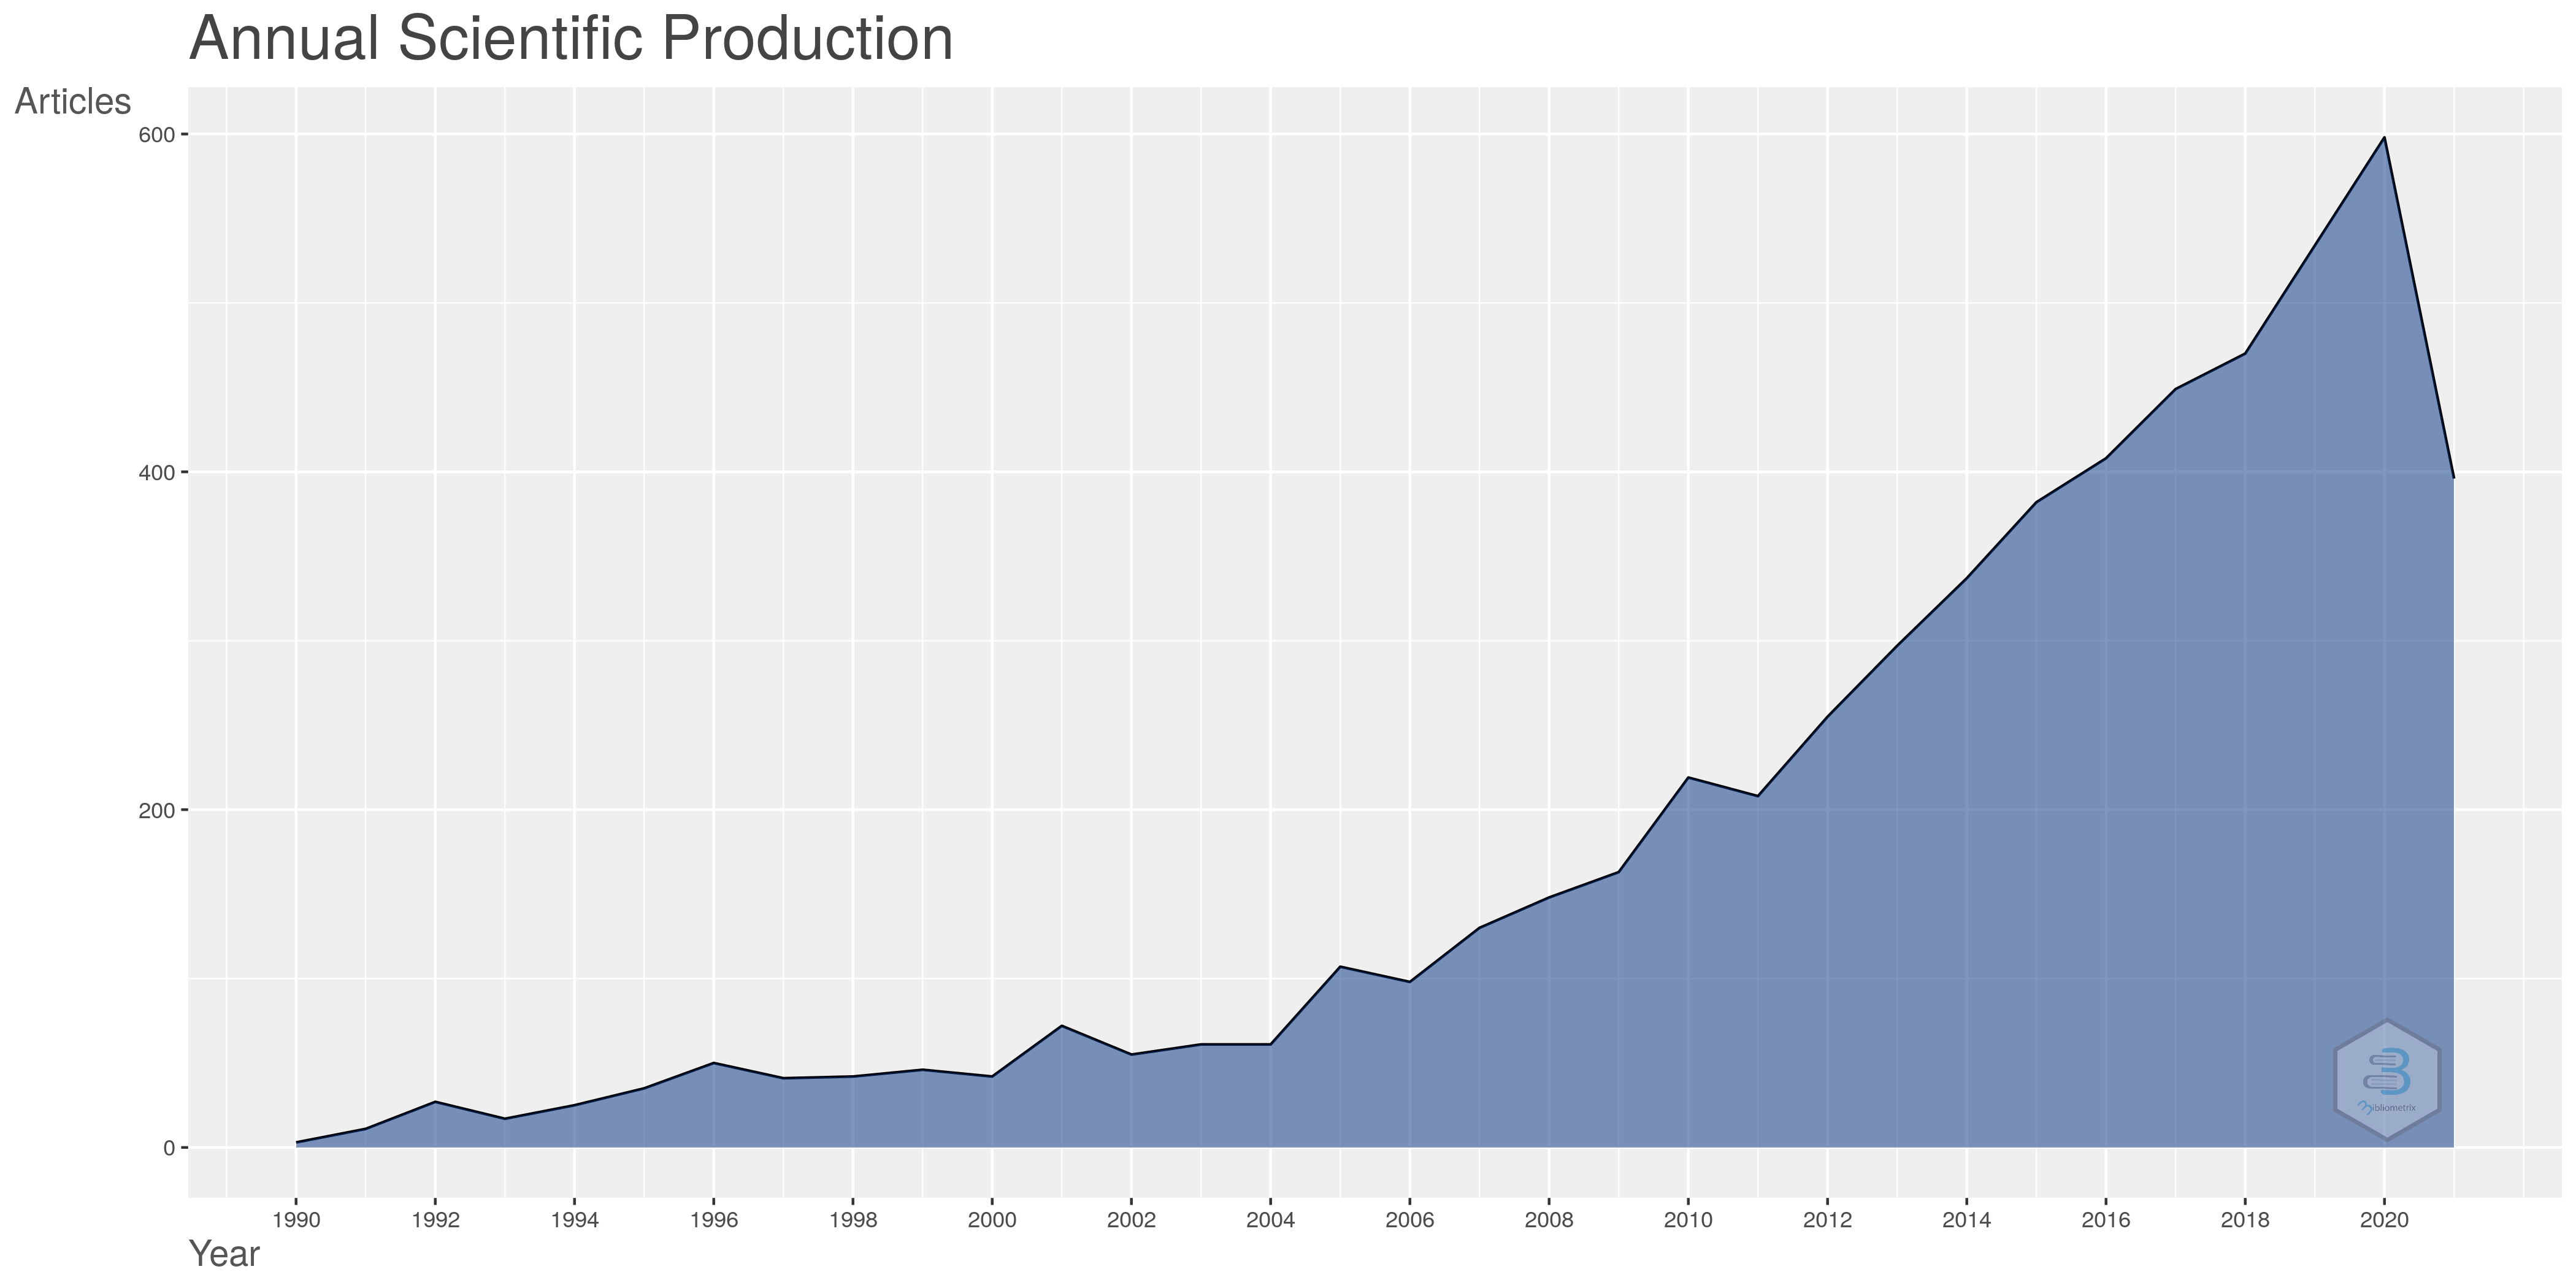
\includegraphics[width=1\textwidth]{experiments/jhcf/PesqBibliogr/Computacao Experimental/WoS-20210803/classico-mais-citacoes/Dataset/AnnualScientificProduction-2021-08-05.png}
    \caption{Evolução da produção científica no dataset MASSA@jhcf.}
    \label{fig:evol:anual:MASSA@jhcf}
\end{figure}

A figura \ref{fig:evol:anual:MASSA@jhcf} apresenta a evolução da produção científica mundial no tema de interesse, segundo o dataset MASSA@jhcf. A curva mostra uma tendência de crescimento aproximadamente exponencial da quantidade de publicações, desde a primeira identificada em 1990.

O \textit{Annual Growth Rate} do dataset é de 17,06\%, bem maior que a taxa média de crescimento da publicação científica mundial, de cerca de 3,3\% anuais, em 2016, como ilustra o estudo em \url{https://www.researchgate.net/publication/333972683_Dynamics_of_scientific_production_in_the_world_in_Europe_and_in_France_2000-2016}, página 23.

\subsection{Interpretação do Crescimento} A maior taxa de crescimento do dataset MASSA@jhcf, bem como o seu grande volume, sugerem que o assunto em pauta desperta intenso interesse, inclusive de ordem econômica.

\subsection{Evolução das Citações}

\begin{figure}
    \centering
    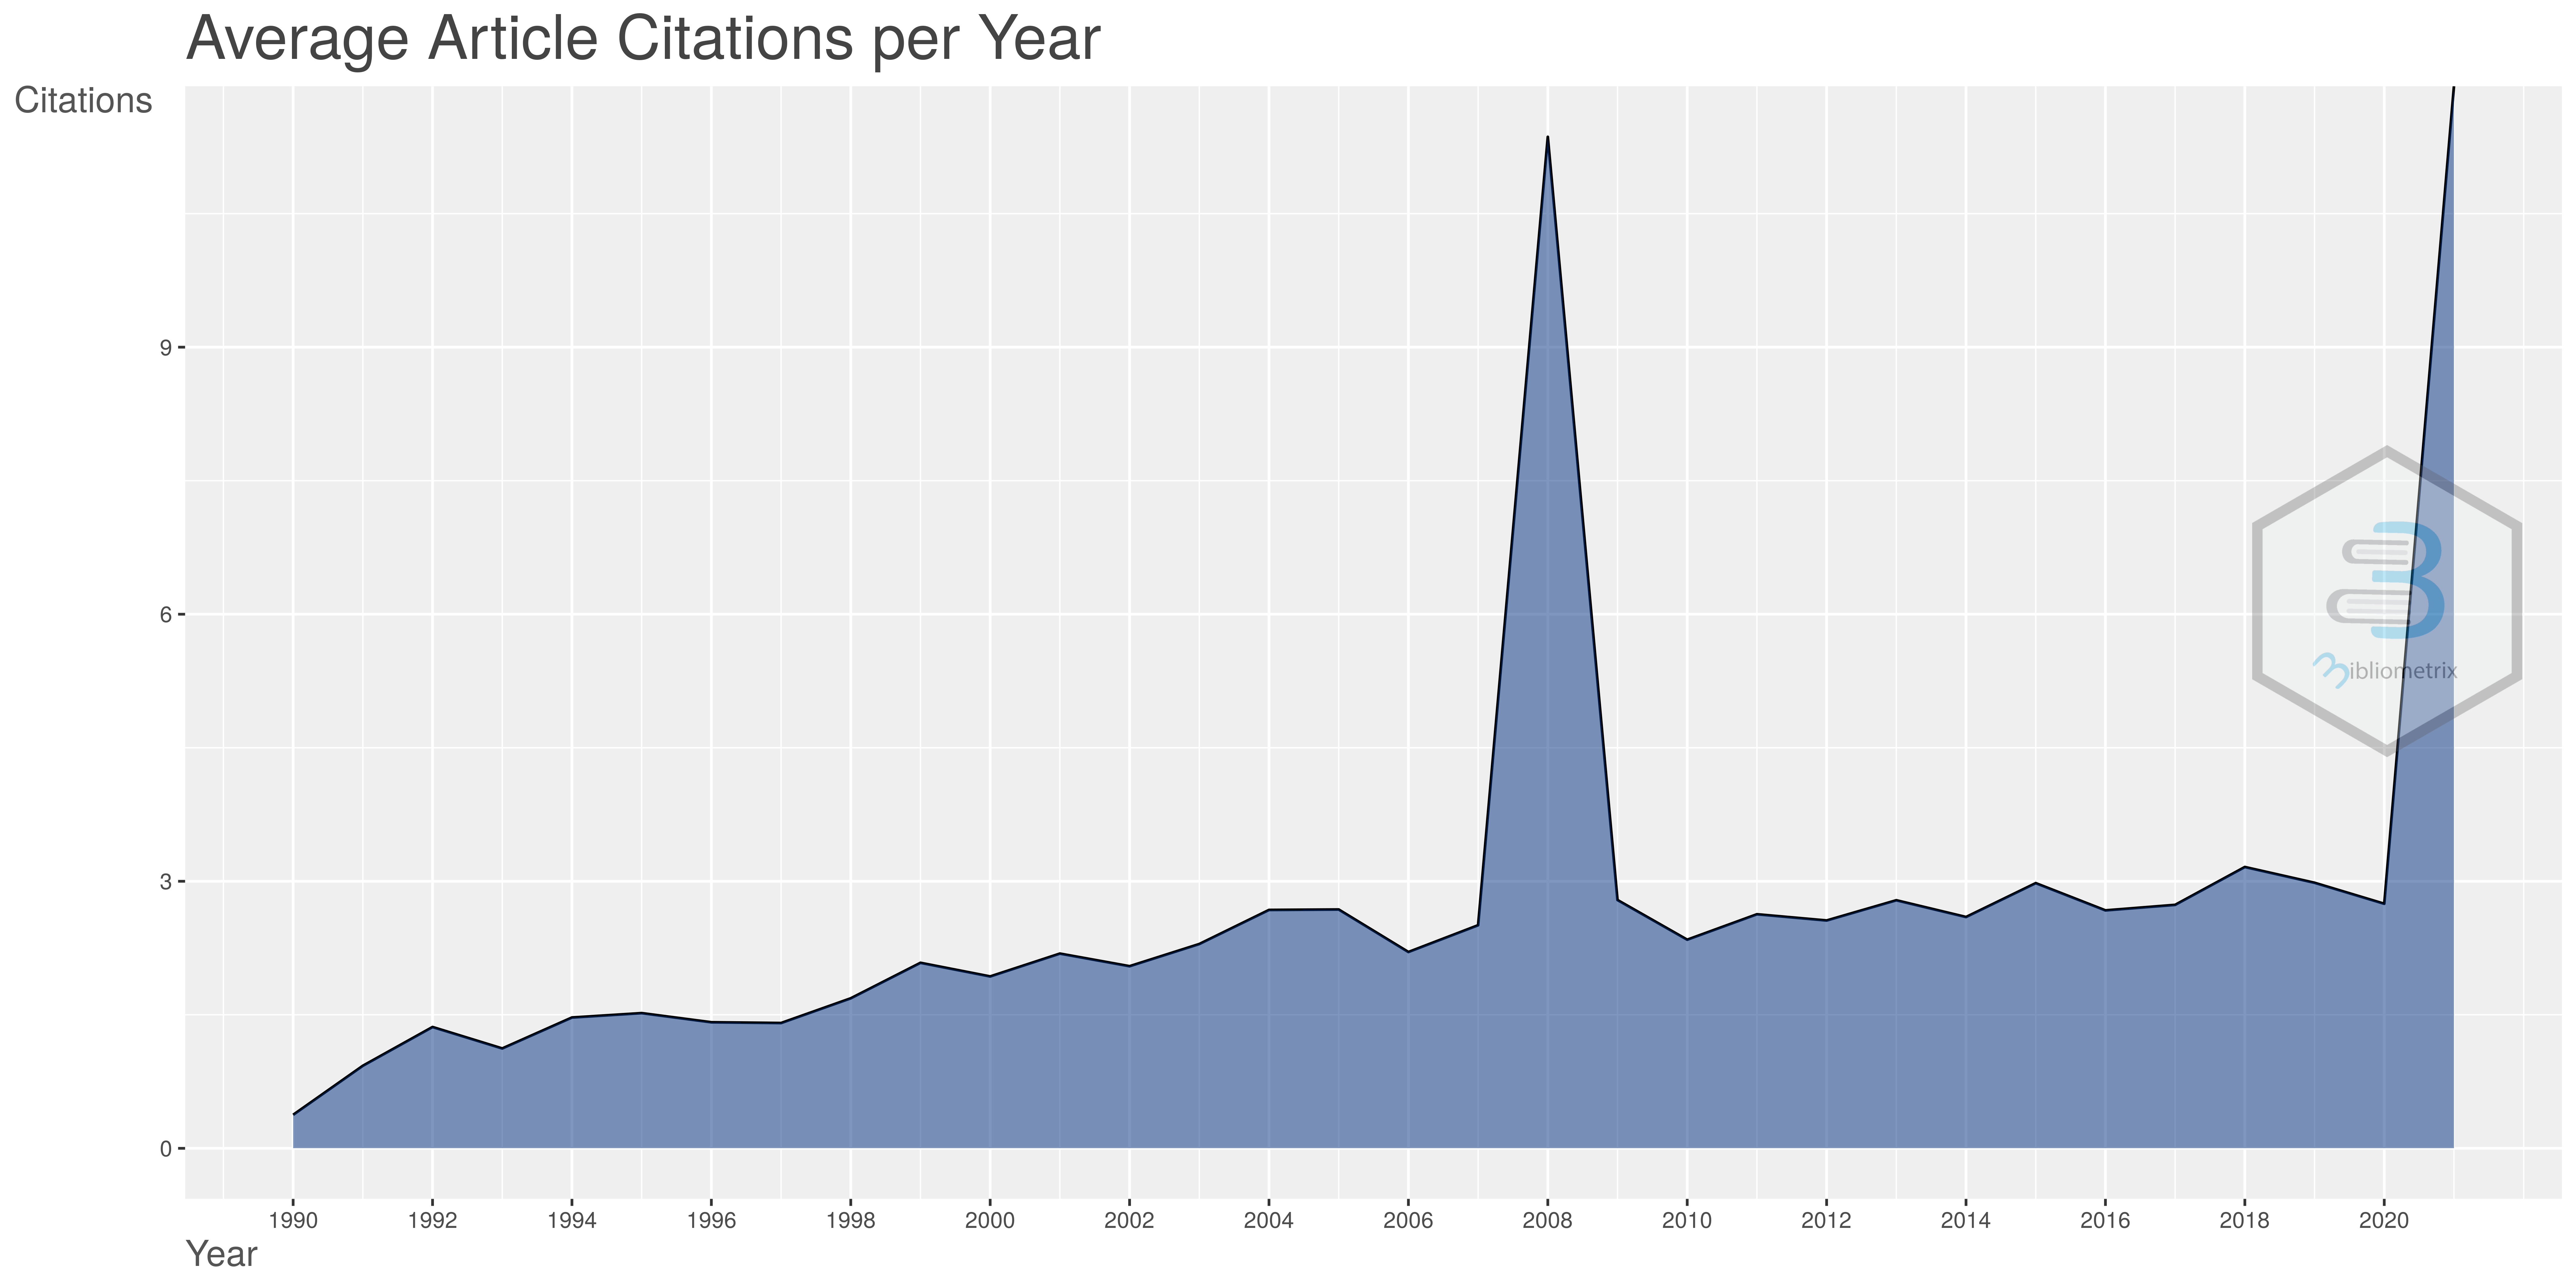
\includegraphics[width=1\textwidth]{experiments/jhcf/PesqBibliogr/Computacao Experimental/WoS-20210803/classico-mais-citacoes/Dataset/AverageArticleCitationPerYear-2021-08-09.png}
    \caption{Evolução das citações ao dataset MASSA@jhcf.}
    \label{fig:evol:anual:citacoes:MASSA@jhcf}
\end{figure}

A figura \ref{fig:evol:anual:citacoes:MASSA@jhcf} apresenta a evolução da média de citações aos 5.787 artigos no dataset MASSA@jhcf. 
Nota-se grande estabilidade na média anual de citações, onde os artigos publicados em 1992 possuem cerca de 2 citações médias, e em 2015 (17 anos depois) o valou alterou-se apenas para três. O pico que aparece no ano de 2008 deve-se, possivelmente, à presença de um artigo do dataset, publicado em 2008, que possui um número surpreendente grande de citações. \footnote{Note que o cálculo do número  médio de citações, nesse caso, utiliza os valores computados no tag "TC (Times Cited)", já presentes no dataset obtido. Ou seja, o gráfico baseia-se no número de citações globais (externas ao dataset MASSA@jhcf), e não no número de citações locais (citações a um artigo do dataset feitas por alguns dos outros artigos dentro do próprio dataset).}.

\subsection{Interpretação das Citações}
Mesmo perante um crescimento aproximadamente exponencial no volume de publicações, a ocorrência de um crescimento nas citações médias ao longo dos anos sugere que os artigos do dataset possuem uma tendência de crescimento no tamanho da bibliografia citada, bem como também despertam grande interesse dos cientistas nas demais áreas do conhecimento (já que se trata de citações globais).

\subsection{\textit{Three-Field Plots (Sankey diagram)}}

As \textit{Three-Field Plots (Sankey diagram)} (plotagens do tipo ``Três Campos'') apresentam afinidades entre três conjuntos de atributos agregados que ocorrem no dataset. Uma plotagem do tipo Sankey busca mostrar os principais fluxos entre diferentes conjuntos de itens. \footnote{Para uma introdução ver \url{https://en.wikipedia.org/wiki/Sankey_diagram}. Para obter detalhes sobre a forma de geração e utilização desse gráfico, inclusive de forma interativa, veja o vídeo em \url{https://www.youtube.com/watch?v=jBb1iha6-sg}.} 

\begin{figure}
    \centering
    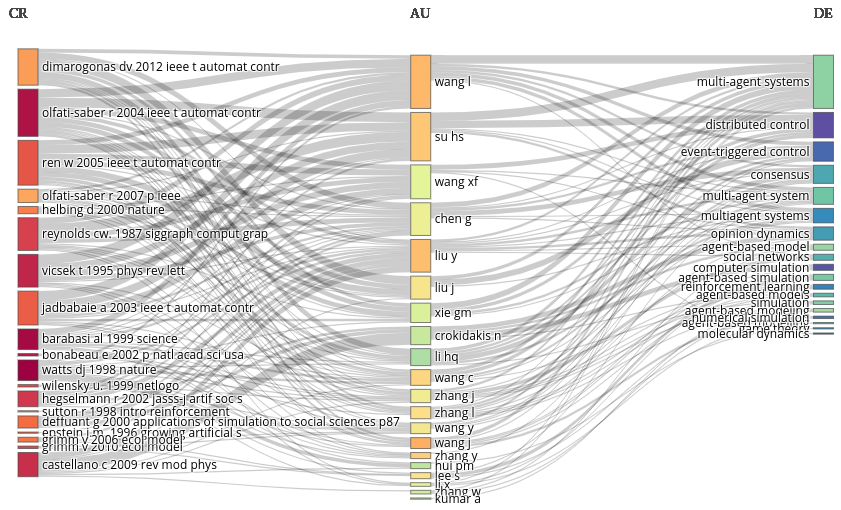
\includegraphics[angle=0,width=1\textwidth]{experiments/jhcf/PesqBibliogr/Computacao Experimental/WoS-20210803/classico-mais-citacoes/Dataset/ThreeFieldPlot-AU-CR-DE-20-20-20.png}
    \caption{Plotagem ``Três Campos'' (Sankey plot) do dataset MASSA@jhcf: 20 Autores, Citações e Palavras-Chave mais proeminentes.}
    \label{fig:MASSA@jhcf:ThreeFieldPlot}
\end{figure}

A figura \ref{fig:MASSA@jhcf:ThreeFieldPlot} apresenta a plotagem do tipo ``Três Campos'' do dataset MASSA@jhcf, vinculando, ao centro, os 20 Autores mais proeminentes (AU), à esquerda, as 20 Citações mais frequentes (CR - Cited Records), e à direita, as 20 Palavras-Chave mais frequentes empregadas pelos autores.

\subsection{Interpretação da figura \ref{fig:MASSA@jhcf:ThreeFieldPlot}}
Os vinte autores mais relevantes, em relação aos artigos mais relevantes citados, e as palavras-chave mais relevantes são aparentemente de origem asiática, mais especificamente chinesa, com base nos sobrenomes. De outra formal, a mesma origem chinesa parece não se aplicar aos trabalhos mais citados, aparentemente europeus ou norte-americanos. Isso sugere estar ocorrendo uma migração recente da produção científica, do ocidente para o oriente. 

Adicionalmente, dentre as palavras-chave (DE) não relacionadas diretamente aos termos de busca, emergem os termos \textbf{distributed control}, \textbf{event-triggered control}, \textbf{consensus} e \textbf{opinion dynamics}. Isso sugere foco das pesquisas por autores de origem chinesa no uso de simulação multiagente voltada à compreensão dos fenômenos de controle social distribuído, formação de consenso e dinâmica da opinião (pública?).

Ainda sobre a interpretação da plotagem da figura \ref{fig:MASSA@jhcf:ThreeFieldPlot}, observa-se que os artigos mais citados encontram-se publicados pelo menos 10 anos atrás, sugerindo que não houve, nos últimos 10 anos, nenhum trabalho que tenha produzido uma mudança de paradigma no tema.
A fim de melhor evidenciar as citações mais relevantes segundo o peso dos autores e palavras-chave, o gráfico da figura \ref{fig:MASSA@jhcf:ThreeFieldPlot:10-20-20} plota apenas as 10 referências citadas, para 20 autores e palavras-chave mais proeminentes.

\begin{figure}
    \centering
    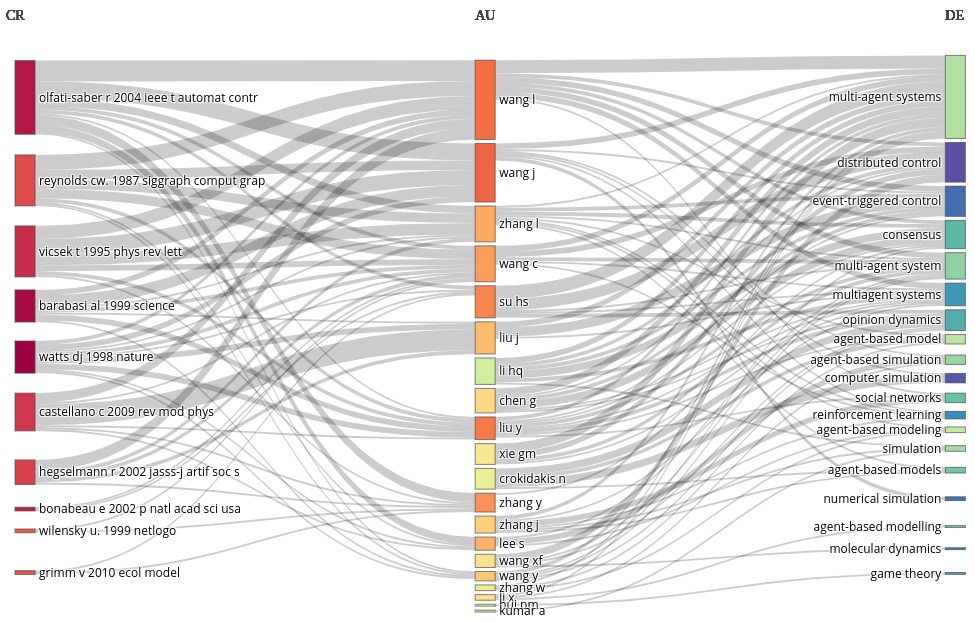
\includegraphics[angle=0,width=1\textwidth]{experiments/jhcf/PesqBibliogr/Computacao Experimental/WoS-20210803/classico-mais-citacoes/Dataset/ThreeFieldPlot-AU-CR-DE-20-10-20.png}
    \caption{Plotagem ``Três Campos'' (Sankey plot) do dataset MASSA@jhcf: 10 Autores, 20 Citações e Palavras-Chave mais proeminentes.}
    \label{fig:MASSA@jhcf:ThreeFieldPlot:10-20-20}
\end{figure}

Breves comentários sobre cada um desses trabalhos serão tratados em seção posterior.

\begin{itemize}
    \item  \cite{olfati-saber_consensus_2004} apresentam discussões teóricas sobre a formação de consenso em sistemas multi-agentes com topologias variáveis;
    \item  \cite{reynolds_flocks_1987} apresenta modelos multi-agentes para simulação gráfica do movimento de rebanhos ou agregados de animais.
    \item \cite{vicsek_novel_1995} analisam a emergência de fenômenos de transição de fase em simulações de de partículas com comportamento autônomo com interação biologicamente motivada.
    \item \cite{barabasi_emergence_1999} investigam a emergência da distribuição livre de escala (\textit{scale-free}\footnote{Ver introdução em \url{https://en.wikipedia.org/wiki/Scale-free_network}.}) em redes que evoluem com base em ligação preferencial.
    \item \cite{watts_collective_1998} exploram o surgimento de redes do tipo mundo pequeno (\textit{small world}\footnote{Ver introdução em \url{https://en.wikipedia.org/wiki/Small-world_network}.}) formadas a partir da reorganização aleatória de redes biológicas, genéticas e outras formas de redes auto-organizadas.
    \item \cite{castellano_statistical_2009} exploram de que forma as técnicas de análise e simulação já usadas na física-estatística podem ser usadas para explicar vários fenômenos sociais, tais como comportamento de multidões, dispersão social, comportamento de multidões etc. Eles apresentam as afinidades entre os dados gerados pelos modelos simulados e dados empíricos obtidos junto a sistemas sociais reais. 
    \item \cite{hegselmann_opinion_2002} exploram a emergência de fenômenos de consenso, polarização e fragmentação da opinião na simulação de sociedades artificiais.
    \item \cite{bonabeau_agent-based_2002} apresenta os potenciais e campos de aplicação da técnicas de simulação baseada em agentes.
    \item \cite{wilensky_netlogo_1999} apresentam a linguagem e ambiente de simulação NetLogo.
    \item \cite{grimm_standard_2006} apresenta o protocolo ODD, proposto para padronizar a descrição de modelos de simulação multiagente.
\end{itemize}

Nenhum desses 10 documentos citados está contido no dataset recuperado.

\subsection{Análises Bibliométricas: Fontes de Informação}

\begin{figure}
    \centering
%    \includegraphics[angle=0,width=1\textwidth]{}
    \caption{Plotagem ``Três Campos'' (Sankey plot) do dataset MASSA@jhcf: 20 Autores, Citações e Palavras-Chave mais proeminentes.}
    \label{fig:MASSA@jhcf:ThreeFieldPlot}
\end{figure}

\subsection{Análises Bibliométricas: Autores}

\subsection{Análises Bibliométricas: Documentos}



\chapter{Análise Bibliográfica sobre Processamento de Linguagem Natural, por Lucas de Almeida Bandeira Macedo}

\section{Planejamento do estudo}

Com a vinda de assistentes virtuais, como a Alexa (Amazon), Cortana (Microsoft) ou Siri (Apple), as pessoas costumam se perguntar cada vez mais: "como que esse programa está entendendo o que eu falo?".

Mas não só de assistentes virtuais vive o Processamento de Linguagem Natural (também conhecido como NLP - Natural Language Processing), afinal, qualquer texto ou fala pode ser interpretado por uma máquina e devidamente classificado. Por exemplo, uma aplicação famosa é o "classificador de sentimentos", em que um modelo treinado consegue classificar textos entre sentimentos "positivos" ou "negativos". Com a ascensão do Twitter, uma rede social baseada em pequenos textos de não mais que 280 caracteres, NLP se torna cada vez mais interessante.

Assim, as perguntas que traçam o norte para este estudo são:

\begin{itemize}
    \item Quais os principais conceitos ligados com Processamento de Linguagem Natural?
    \item Como se dá o progresso das pesquisas em NLP ao longo dos anos? As redes sociais influenciaram esse crescimento?
    \item Qual o estado da estrutura social da comunidade de NLP?
\end{itemize}

\subsection{Uso do Bibliometrix e Biblioshiny}

Será usada a ferramenta Bibliometrix, com sua função Biblioshiny, para gerar gráficos e grafos iterativos e personalizáveis, para auxiliar na interpretação da realidade científica do tópico.

\section{Coleta de dados}

A coleta de dados foi feita utilizando o site Web of Science (WoS), no dia 03/02/2022, através do portal periódico da capes.

A pesquisa foi realizada utilizando as edições "Science Citation Index Expanded" e "Conference Proceedings Citation Index – Science", ambas coleções são voltadas para, principalmente, as ciências exatas.

A \textit{string} (ou \textit{query}) de busca inicialmente utilizada foi a seguinte:

\lstinputlisting[numbers=left,basicstyle=\normalsize\ttfamily,caption={Query de busca sobre Processamento de Linguagem Natural.},label=queryNLPABM1]
{experiments/ABMHub/PesquisaBibliometrica/NLP/pesquisa_velha.txt}

\subsection{Explicação para os termos de busca usados}
\label{sec:ABMHub:query}

A proposta é apenas pesquisar sobre Processamento de Linguagem Natural, sem muito rigor na aplicação em que essa arquitetura de rede neural é aplicada. Portanto, inicialmente a pesquisa foi apenas "natural language processing".

Porém, uma rápida olhada pelos artigos retornados evidenciou uma grande quantidade de artigos sobre linguísticas, e áreas que não são da computação. Como o objetivo aqui adquirir modelos de Deep Learning, a pesquisa foi ajustada para filtrar apenas por NLP ligadas diretamente a computação e inteligência artificial, evidenciado pelas cláusulas "neural network", "(machine or deep) and learning" e "artificial intelligence". Essa nova pesquisa trouxe melhores resultados, todos evidenciando redes neurais e variadas técnicas de machine learning. O total de registros retornado pela query foi 10152, e esse dataset será, daqui para frente, mencionado como "\textit{NLP@LABM}".

\subsubsection{Refinamento da Coleta de Dados}
\label{sec:abmhub:refinamento}

 Em seguida, em uma análise mais fina, utilizando a \textbf{Rede de Co-ocorrências de Palavras-chave}, podemos evidenciar outras palavras chaves que estavam aparecendo entre os registros da pesquisa, que não deveriam estar aparecendo. É possível observar na imagem \ref{fig:ABMHub:NLPgraph1}, palavras como "câncer" ou "diagnóstico" que estão relacionadas a visão computacional mais que NLP, aparecendo com pesos não-desprezíveis.
 
 \begin{figure}
    \centering
    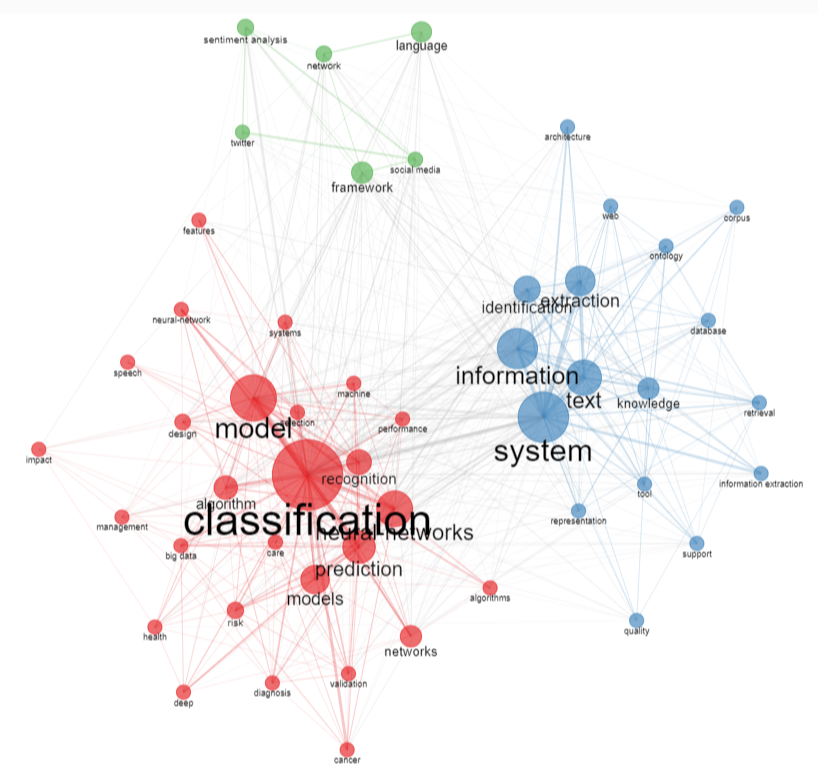
\includegraphics[width=1\textwidth]{experiments/ABMHub/PesquisaBibliometrica/NLP/grafo_keywords.png}
    \caption{Grafo de relação de keywords do dataset \textit{NLP@LABM}}
    \label{fig:ABMHub:NLPgraph1}
\end{figure}

Assim, é necessário uma nova iteração da pesquisa, para evitar que registros de visão computacional corrompam a pesquisa de NLP. É delicado fazer isso, pois existem muitas menções a Visão Computacional nos registros de LP, já que ambos são ligados a Deep Learning, então retirar a keyword "Visão Computacional" provavelmente removeria muitos registros que não gostaríamos de remover da pesquisa. Assim, a melhor solução encontrada foi remover palavras que não têm intersecção entre os dois assuntos. Por exemplo, "medical", "cancer" e "diagnosis".

Assim, chegamos na mais recente query:

\lstinputlisting[numbers=left,basicstyle=\normalsize\ttfamily,caption={Query refinada de busca sobre Processamento de Linguagem Natural.},label=queryNLPABM2]
{experiments/ABMHub/PesquisaBibliometrica/NLP/pesquisa_nova.txt}

Esta query refinada retornou 8557 registros, e esse novo dataset, que será usado ao longo desse estudo, é nomeado de \textit{NLP2@LABM}.

\subsection{Filtragem de registros}

Após o refino, foi estabelecido que usaremos o dataset \textit{NLP2@LABM} de 8557 registros. Portanto, podemos começar a tratá-lo e analisá-lo. Para isso, começamos filtrando registros indesejados, como prévias de artigos, críticas sobre outros arquivos, cartas e etc. Assim, deixaremos apenas os artigos, pois é o método padrão de publicação científica, e capítulos de livros, já que é um tipo de publicação recorrente na área. Após o filtro, reduzimos nosso dataset para 3308 registros.

\subsection{Análise descritiva do \textit{dataset} \textit{NLP2@LABM}}

Ainda utilizando a ferramenta Bibliometrix, faremos uma análise descritiva do dataset adquirido, ou seja cálculos de diversas métricas para trazer \textit{insights}.

\begin{description}
    \item [\textit{Timespan}] De 1990 até 2022 (hoje). Não foram encontrados registros de 1945 até 1989.
    \item [\textit{Sources (Journals, Books, etc)}] 750 fontes diferentes de artigos.
    \item [\textit{Average years from publication}] A média do tempo de publicação dosartigos no dataset é de 3,85 anos.
    \item [\textit{Average citations per documents}] Cada artigo foi citado em média 14.03 vezes.
    \item [\textit{Average citations per year per doc}] Os artigos do dataset por inteiro são, em média, citados 2567 vezes por ano.
    \item [\textit{References}] Os artigos têm 108452 referência para outras fontes.
    \item [\textit{Keywords Plus (ID)}] Há 2414 diferentes palavras chaves.
    \item [\textit{Author's Keywords (DE)}] Há 7439 diferentes palavras chaves, segundo os autores.
    \item [\textit{Authors}] Há 10028 diferentes autores.
    \item [\textit{Author Appearances}] Há 13237 autores (considerando repetição nomes para diferentes artigos).
    \item [\textit{Authors of single-authored documents}] Há 154 autores que fizeram trabalhos sozinhos.
    \item [\textit{Authors of multi-authored documents}] Há 9874 autores que fizeram trabalhos com outras pessoas.
    \item [\textit{Single-authored documents}] Há 163 trabalhos com apenas um autor.
    \item [\textit{Documents per Author}] Há, em média, 0,33 autores por trabalho.
    \item [\textit{Authors per Document}] Há, em média, 3,03 trabalhos por autor.
    \item [\textit{Co-Authors per Documents}] As 13237 aparições de autores se distribuem, em média 4 vezes para os 3308 documentos do dataset.
    \item [\textit{Collaboration Index}] Os autores que editaram artigos com um ou mais co-autores, colaboraram em media 3,54 vezes para editar os elaborados em co-autoria.
\end{description}

\subsection{Evolução da Produção Científica}

A evolução da produção científica do assunto é um dos principais motivadores dessa pesquisa. Afinal, com a quantidade absurda de dados que existem hoje livremente disponíveis na internet (e em exponencial crescimento), provavelmente influencia muito a qualidade de modelos gerados em qualquer área de machine learning. É esperado que, motivado por essa crescente de dados, e com a popularização de assistentes virtuais, NLP seja um tópico cada vez mais estudado.

 \begin{figure}
    \centering
    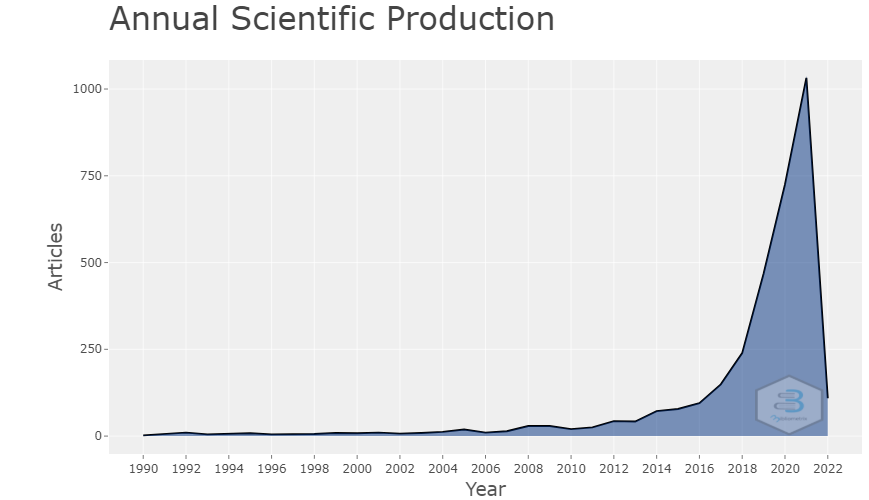
\includegraphics[width=1\textwidth]{experiments/ABMHub/PesquisaBibliometrica/NLP/anualScientificProduction.png}
    \caption{Produção científica anual sobre o \textit{dataset} \textit{NLP2@LABM}}
    \label{fig:ABMHub:ASP}
\end{figure}

Podemos ver que as suposições anteriores são verdadeiras (ou, ao menos, aparentemente verdadeiras). Como visto na figura \ref{fig:ABMHub:ASP}, a crescente absurda e exponencial em deep learning entre 2016 e 2021 realmente dá pistas que NLP está cada vez mais relevante no mundo moderno, e que continuará crescendo em influência por um bom tempo. É importante ressaltar que a queda apresentada no fim do gráfico ocorre apenas porque esses registros foram extraídos no começo do ano 2022.

Também é interessante observar que o primeiro registro é em 1990. O conceito de NLP foi inventado antes dessa data, mas apenas a partir desse ponto que NLP começou a ser estudado junto com Machine Learning, e a query utilizada (seção \ref{sec:ABMHub:query}) especifica que é necessária a ligação de processamento de linguagem natural com inteligência artificial.

\subsection{Evolução das Citações}

 \begin{figure}
    \centering
    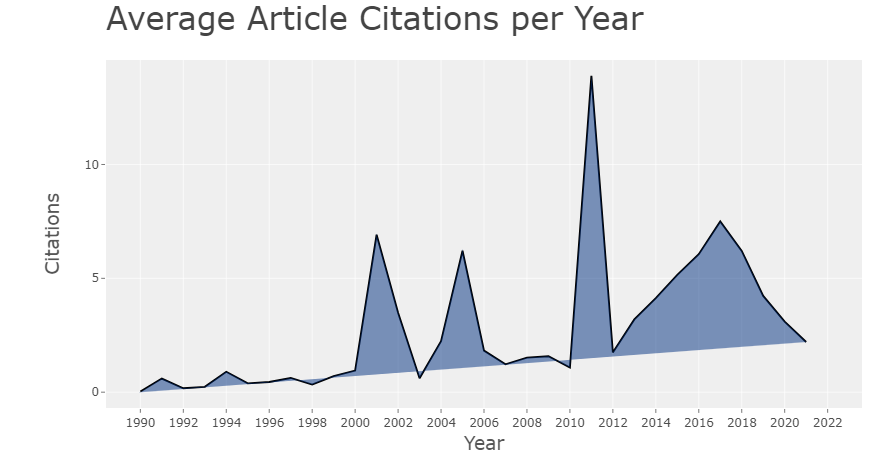
\includegraphics[width=1\textwidth]{experiments/ABMHub/PesquisaBibliometrica/NLP/citationsPerYear.png}
    \caption{Produção científica anual sobre o \textit{dataset} \textit{NLP2@LABM}}
    \label{fig:ABMHub:CPY}
\end{figure}

Podemos perceber que há um claro crescimento médio desde 1990 das citações médias por ano. Uma das coisas que mais chama atenção são os 4 picos no gráfico: em 2001, 2005, 2011 e 2017. Esses provavelmente são de artigos (ou grupos de artigos) que tiveram um impacto fora do comum, trazendo novos conceitos ou realizando descobertas fantásticas.

Esta é, inclusive, uma das perguntas feitas como motivação de pesquisa: "Como se dá o progresso das pesquisas em NLP ao longo dos anos? As redes sociais influenciaram esse crescimento?". Vemos que há crescimento mas, exclusivamente através desses dados, é difícil tirar conclusões sobre a relação deste crescimento com a vinda de redes sociais. 

\subsection{\textit{Three-Field Plots (Sankey diagram)}}

Como o nome indica, "Three-Field Plots" são tipos de gráficos que buscam correlacionar três tipos de dados diferentes, sem a necessidade de uma terceira dimensão adicionada em cima de um gráfico bidimensional. Na imagem \ref{fig:ABMHub:TFP}, temos um exemplo de plotagem de três campos que interliga os autores presentes no \textit{dataset} \textit{NLP2@LABM}, com fontes que eles citaram, assim como palavras chaves que costumam usar em seus artigos. 

 \begin{figure}
    \centering
    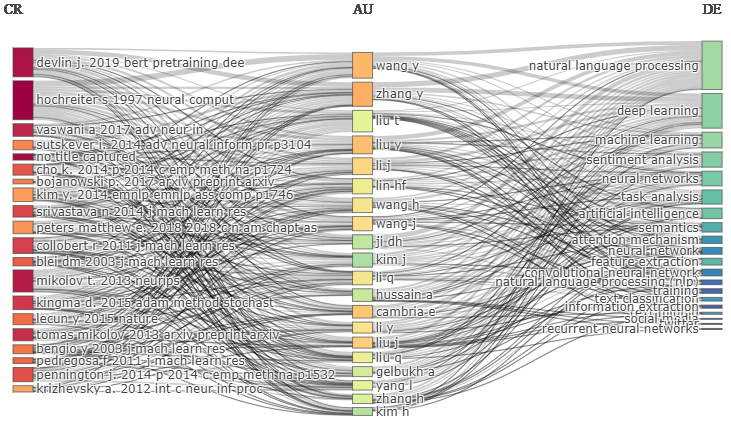
\includegraphics[width=1\textwidth]{experiments/ABMHub/PesquisaBibliometrica/NLP/tfp1.png}
    \caption{Three Field Plot - Citações, Autores e Palavras chaves sobre o \textit{dataset} \textit{NLP2@LABM}}
    \label{fig:ABMHub:TFP}
\end{figure}

Nessa plotagem, podemos extrair algumas informações muito interessantes sobre o estado atual de NLP. Primeiramente, vemos que o artigo mais citado por todos os artigos do \textit{dataset} aqui apresentado é sobre computação neural (ou redes neurais), o que faz muito sentido, considerando que a NLP moderna é baseada em machine e deep learning. Outra observação interessante é que os artigos, em geral, são igualmente citados, mostrando que existe uma série de conceitos base para a NLP que são usados na maioria das aplicações do conceito.

Outro ponto interessante é que quase todos os autores listados no gráfico são chineses. Isso evidencia muito claramente a ascensão da China como potencia intelectual e tecnológica, principalmente em uma área tão relevante como a Inteligência Artificial.

Por último, as keywords também merecem sua atenção. Como esperado por ser o foco do \textit{dataset} \textit{NLP2@LABM}, Processamento de Linguagem Natural é a palavra-chave com mais menções. Mas, em seguida, vemos "Deep Learning", "Machine Learning" e "Neural Networks", o que faz muito sentido, partindo do princípio que (como dito anteriormente), NLP se apoia nesses conceitos atualmente. Também temos, com tamanho considerável, "sentiment analysis" e "task analysis", que são aplicações muito famosas de NLP.

\subsection{Análise da estrutura conceitual}

Nessa seção, analisaremos mais profundamente a estrutura conceitual do dataset \textit{NLP2@LABM}, afinal, essa é uma das perguntar norteadoras da pesquisa, então deve ser respondida com muita clareza. Essa análise ocorrerá pela análise de correspondência de keywords, parecido com a análise presente na seção \ref{sec:abmhub:refinamento}.

 \begin{figure}
    \centering
    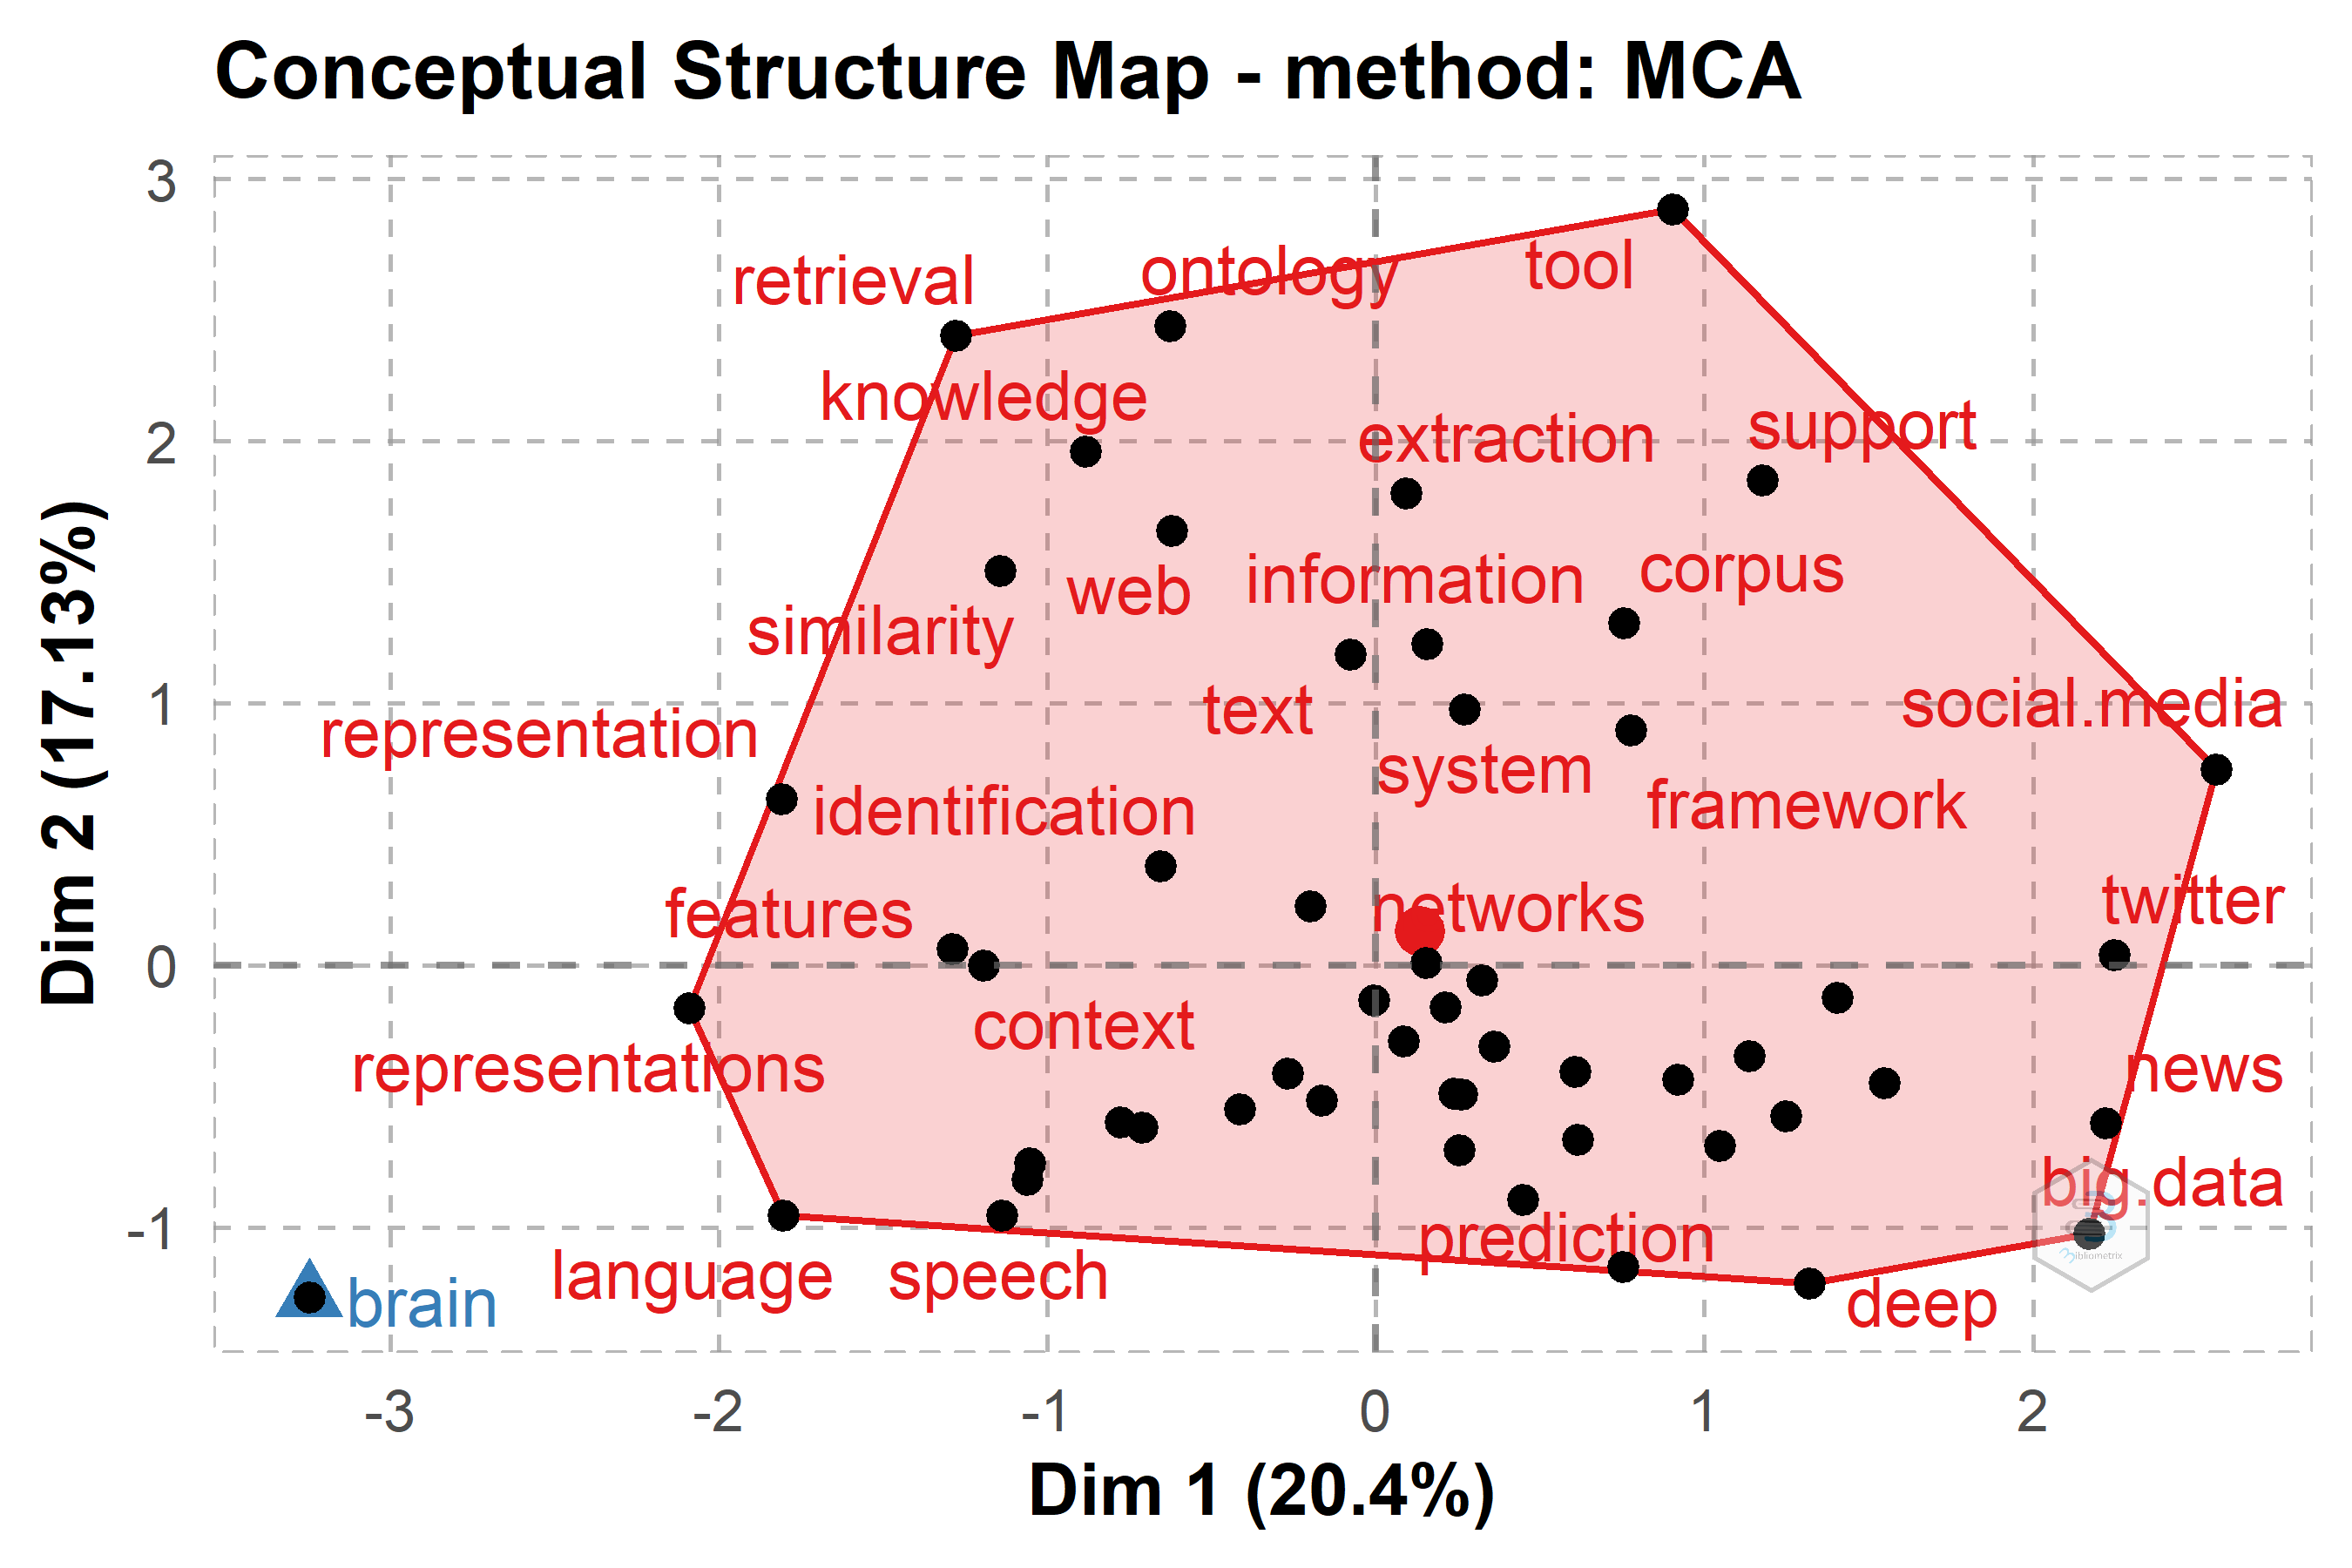
\includegraphics[width=1\textwidth]{experiments/ABMHub/PesquisaBibliometrica/NLP/estruturaConceitual.png}
    \caption{Estrutura conceitual do dataset\textit{NLP2@LABM}}
    \label{fig:ABMHub:EC}
\end{figure}

Podemos observar que há uma grande correlação entre todos os tópicos presentes no dataset. Era de se esperar, pois NLP está intrinsecamente e igualmente ligado com com conceitos como extração (de dados), deep learning, fala, linguagem, conhecimento, etc. Todos esses conceitos caminham juntos quando o assunto é NLP, pois todos eles compõem ou são produtos de NLP.

Mas existe um ponto no canto inferior esquerdo, em um agrupamento separado do agrupamento principal, com a label "brain". Um único tópico é pouco para definir o que exatamente esse ponto representa, portanto, é necessário forçar mais pontos no mapa para tentar traçar um padrão.

 \begin{figure}
    \centering
    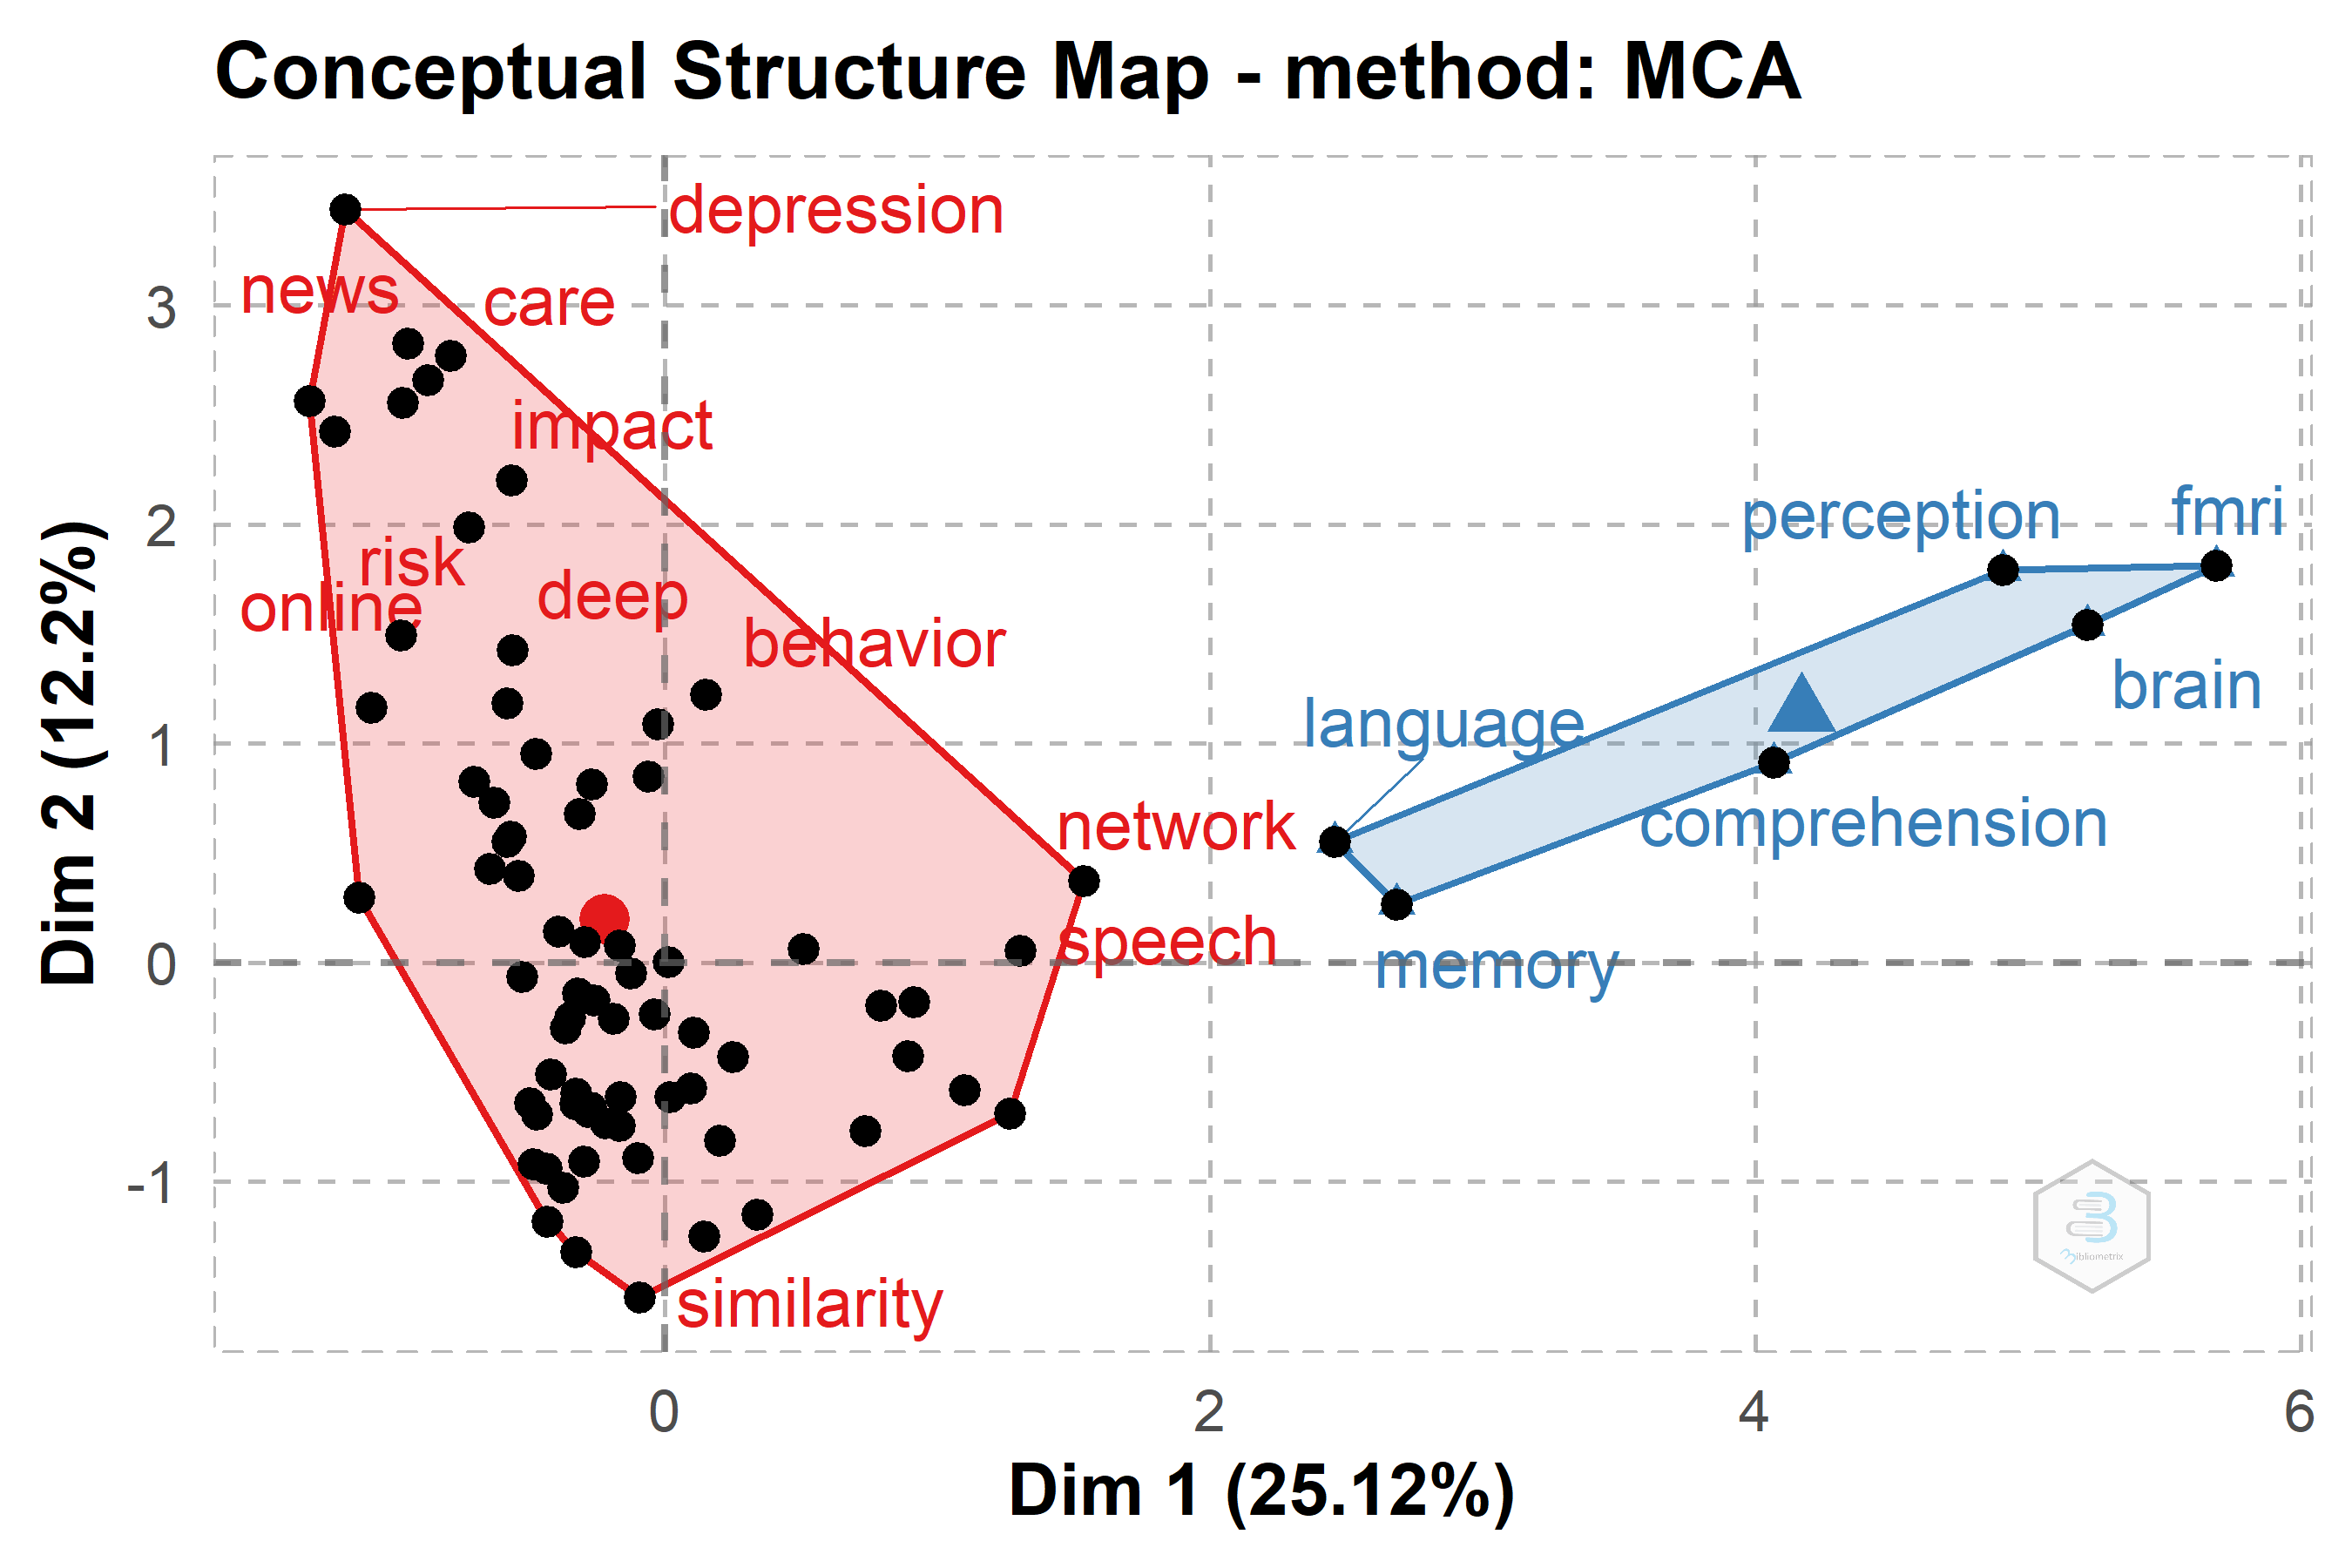
\includegraphics[width=1\textwidth]{experiments/ABMHub/PesquisaBibliometrica/NLP/estruturaConceitual2.png}
    \caption{Estrutura conceitual com 100 nós do dataset\textit{NLP2@LABM}}
    \label{fig:ABMHub:EC2}
\end{figure}

Conseguimos ver, na figura \ref{fig:ABMHub:EC2}, o que aquele ponto representava: um cluster de estudos da mente. Tópicos como memória, compreensão, cérebro, percepção, linguagem, etc, podem representar duas vertentes: estudiosos que tentam usar ferramentas de deep learning para progredir nos estudos da mente (afinal, redes neurais são inspiradas no comportamento do cérebro), e estudiosos que usam os conhecimentos da mente para progredir nos estudos de deep learning (pelo mesmo motivo que o anterior). Em ambos os casos, é interessante ver esse cluster no dataset.

\subsection{Análise da estrutura social}

A última pergunta que devemos responder, e ainda não foi respondida, é sobre a estrutura social da comunidade de NLP. Para isso, daremos uma olhada na rede de colaborações do dataset \textit{NLP2@LABM}, relacionando os países entre si (figura \ref{fig:ABMHub:social}).

\begin{figure}
    \centering
    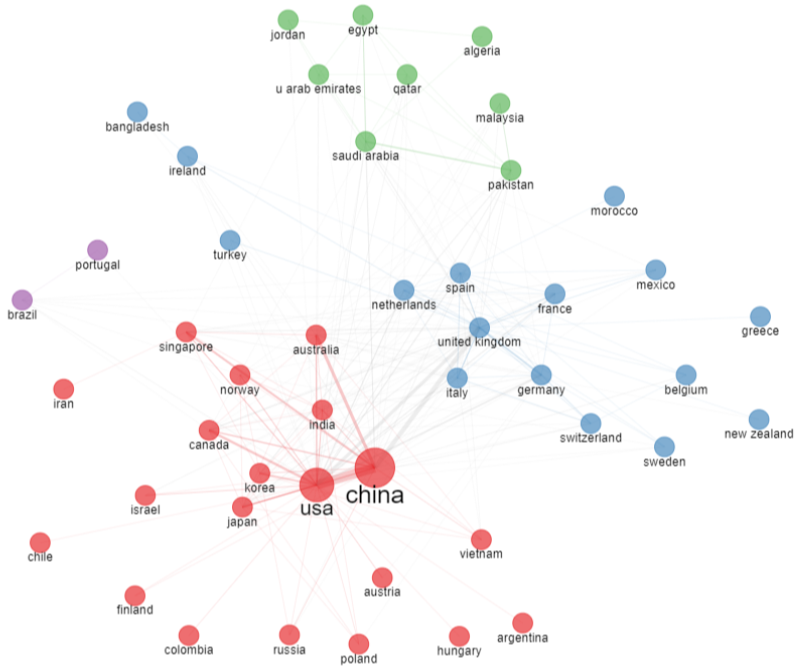
\includegraphics[width=1\textwidth]{experiments/ABMHub/PesquisaBibliometrica/NLP/socialStructure.png}
    \caption{Estrutura social de países do dataset\textit{NLP2@LABM}}
    \label{fig:ABMHub:social}
\end{figure}

Podemos ver, imediatamente, que as duas grandes potencias da área são Estados Unidos e China. Isso já era esperado, pois são as duas maiores potencias da ciência, como um todo. Nesse mesmo cluster, conseguimos encontrar outros países desenvolvidos, como Japão e Canadá, que costumam também ser grandes contribuintes para a ciência mundial. O cluster em azul, por outro lado, já apresenta uma reunião de países majoritariamente europeus, com algumas exceções de países emergentes, como Brasil e Rússia. Finalmente, o último cluster da imagem apresenta países majoritariamente do oriente médio, e contêm menos ligações que os outros dois clusters.

Com essa dominância absoluta da China e dos Estados Unidos sobre os outros países, fica a pergunta: como essa divisão de conhecimento é feita internamente no país? O grafo da figura \ref{fig:ABMHub:social2} responde essa pergunta.

\begin{figure}
    \centering
    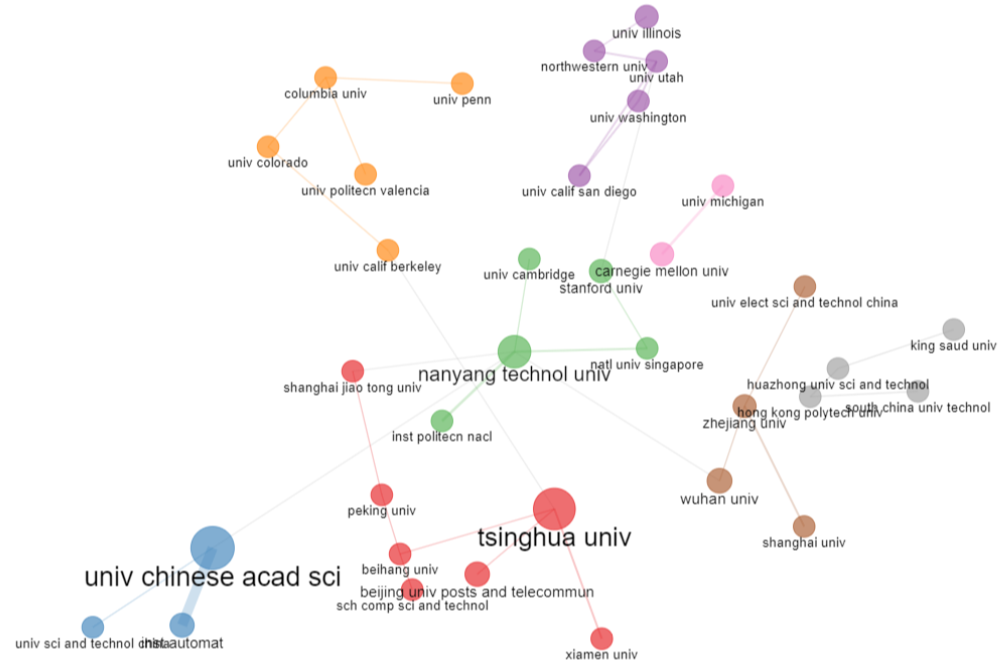
\includegraphics[width=1\textwidth]{experiments/ABMHub/PesquisaBibliometrica/NLP/socialStructure2.png}
    \caption{Estrutura social de universidades do dataset\textit{NLP2@LABM}}
    \label{fig:ABMHub:social2}
\end{figure}

Podemos ver que há, na China, uma concentração muito alta de conhecimento em uma pequena quantidade de universidades. Seguindo o sentido contrário, nos Estados Unidos, o conhecimento é muito mais diluído entre várias universidades diferentes. O interessante desses dois países é que, como visto na figura \ref{fig:ABMHub:social}, os dois países apresentam uma quantidade quase igual de artigos publicados, mas a divisão de conhecimento interno aos países é absolutamente diferente.

Uma última análise no quesito social é descer mais um nível e olhar o grafo de relação entre diferentes autores (figura \ref{fig:ABMHub:social3}).

\begin{figure}
    \centering
    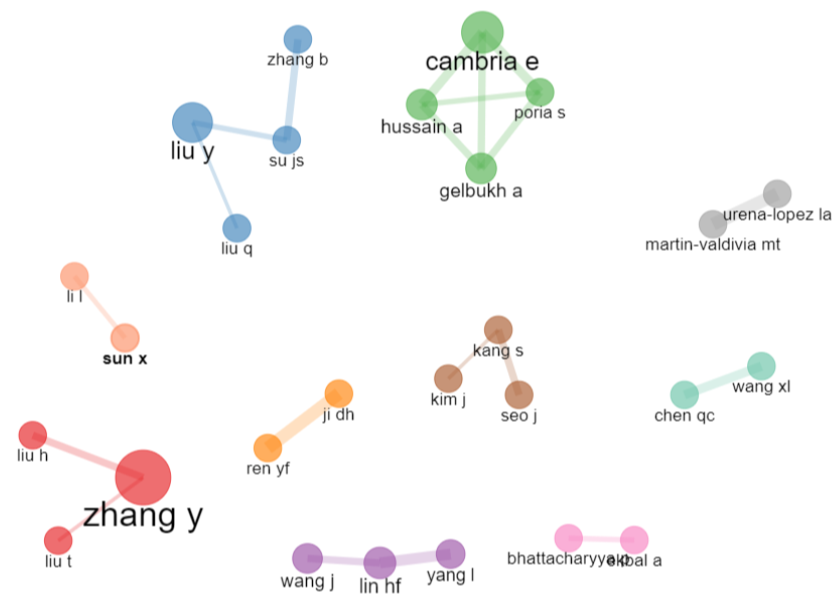
\includegraphics[width=1\textwidth]{experiments/ABMHub/PesquisaBibliometrica/NLP/socialStructure3.png}
    \caption{Estrutura social entre autores do dataset\textit{NLP2@LABM}}
    \label{fig:ABMHub:social3}
\end{figure}

Podemos observar, de imediato, a grande quantidade de estudiosos chineses, e seus grupos com muito impacto na área. Mais da metade dos clusters, e os com maior impacto, são de autores chineses. Porém, o cluster composto de Soujanya Poria, Amir Hussain, Erik Cambria e Alexander Gelbukh é uma exceção a regra. Esses autores são de Singapura, e os 4 têm um impacto muito grande nesse grafo, com vários trabalhos, a maioria com os quatro em grupo.

\section{Conclusões}

Pudemos ver que, como esperado, os estudos de NLP tiveram uma explosão gigantesca recentemente. O gráfico de produção científica apresenta uma curva gigantesca, sendo basicamente uma exponencial. Esse crescimento pode ser explicado de vários jeitos: ascensão da web; assistentes virtuais; tecnologias de acess 

\chapter{Análise Bibliográfica sobre Otimizações algorítmicas para simulações de fenômenos fluídos e óticos por Alexsander Correa de Oliveira}

\section{Planejamento do estudo}
    A indústria de jogos é a que mais cresce dentre todas as formas de entretenimento atuais. Alguns desses jogos podem chegar a investimentos tão grandes que disputam com os filmes mais caros da história. No posto de vista do consumidor, todo tempo e dinheiro gastos são apenas meios para um fim, que é o de ter a melhor experiência possível. Contudo do ponto de vista dos desenvolvedores, esses fatores são consequências de horas e horas de trabalho.
    
    Toda a tecnologia criada para esses jogos tem de ser cada vez mais eficiente, dado a necessidade de tornar os gráficos cada vez mais realistas, e seus mundos ainda mais acreditáveis. As técnicas utilizadas para tal otimização são fortemente baseadas em artigos \emph{state-of-the-art} tanto e física quanto em geometria.
    
    Entre todos aspectos físicos, que hoje em dia são mais prevalentes nos jogos, temos algumas áreas de estudo que pesam mais, principalmente em performance: 
    \begin{itemize}
        \item Corpos fluídos, como água e ar;
        \item Análise de vetores em ótica, para saber como a iluminação afetará um determinado ambiente;
        \item Análise da topologia, com fins de otimizar \emph{path-finding};
    \end{itemize}
\subsection{Uso do Bibliometrix e Biblioshiny}
     Com o auxílio das ferramentas disponibilizadas pelo Bibliometrix, como o Biblioshiny, serão analisados os artigos encontrados, por meio de gráficos e tabelas.   
\section{Coleta de Dados}
    A coleta de dados foi iniciada no dia 02/02/2022, e usou a base Web of Science, com acesso direto pelo periódico Capes.
    
    Por fins de diminuir o tamanho do \emph{dataset}, só foi utilizada a edição \emph{Science Citation Index Expanded}, que tem o foco voltado para ciências exatas e naturais.
    
    A busca inicial foi feita com a seguinte \emph{query}:
\begin{lstlisting}
((algorit* ) and (Optimization)) and 
(optics or ((fluid* or aero*) and dynamics))
\end{lstlisting}
\subsection{Explicação para a \emph{Query}}
    A busca foi feita com o objetivo de encontrar apenas técnicas para otimizar algoritmos relacionados a ótica, aerodinâmica e hidrodinâmica.
    
    Os termos $((algorit* ) and (Optimization))$ são para encontrar apenas os artigos relacionados a algoritmos computacionais.
    
    Já $(optics or ((fluid* or aero*) and dynamics))$ serve para falar que tanto faz um artigo de ótica ou de aerodinâmica ou de hidrodinâmica.
    
    Com a \emph{Query} já montada, os registros foram exportados do WoS com todas as informações disponíveis e no formato de arquivo de texto sem formatação. Foram recuperados desa maneira, 7443 registros no total.
\section{Análise dos dados}
    Uma análise inicial foi feita com o objetivo de retirar artigos indesejados. Para atingir isso, foi utilizado o gráfico \emph{Co-occurrence Network}, que mostra as palavras com maior peso, e o relacionamento entre elas.
    
     \begin{figure}
    \centering
    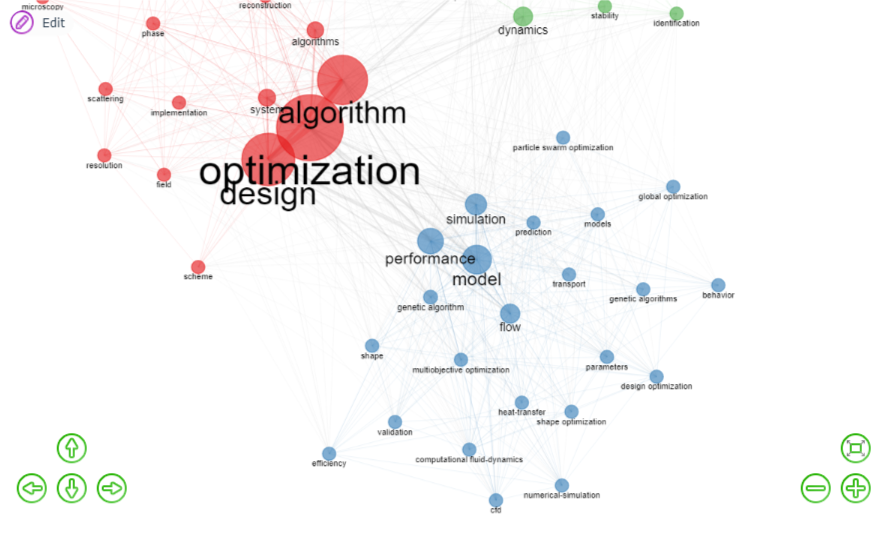
\includegraphics[width=1\textwidth]{experiments/KvotheKS/PesqBibliogr/AlgoritmosSimulacaoOptica-Dinamica/WoS-20220202/OldQueryDataset/CoOccurrence.png}
    \caption{Rede de co-ocorrência}
    \label{fig:KvotheKS:OldQueryCoOccurrence}
\end{figure}
    
    Destacando um dos lados do grafo e o meio, podemos ver que o foco em computação e otimização foram atingidos. Contudo, como um efeito não desejado, também foram "recebidos" artigos que envolvem I.A, como também ótica de um ponto de vista médico.
    
\subsection{Refinamento dos Dados}
    Para retirar todo produto indesejado foi feita uma nova \emph{query} na mesma base e edição:
    
\begin{lstlisting}[basicstyle = \normalsize]
((algorit* ) and (Optimization)) and 

(optics or ((fluid* or aero*) and dynamics))

not ((genetic* and algorit*) or medic* or (machin* and learn*))
\end{lstlisting}

    Com os novos parâmetros, o objetivo de retirar tudo relacionado a medicina e a maioria de algoritmos genéticos foi atingido. Como resultado da nova busca, foram retornados 4917 elementos. Contudo, considerando apenas o número de artigos, o número cai para 4859.
    
    Como demonstração da melhora do \emph{dataset}, segue o gráfico \ref{fig:KvotheKS:Final_Data_Set}:
    
    \begin{figure}[H]
    \centering
    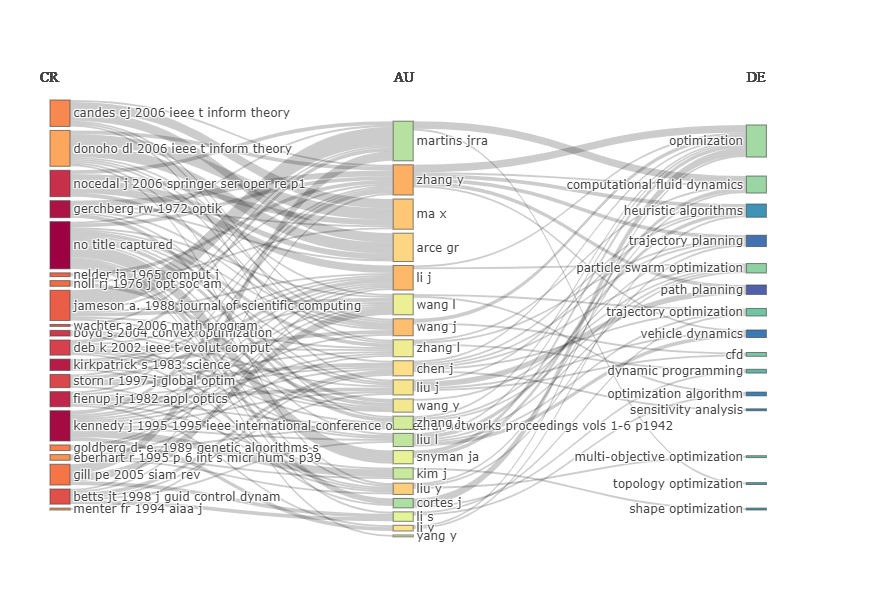
\includegraphics[width=1.3\textwidth]{experiments/KvotheKS/PesqBibliogr/AlgoritmosSimulacaoOptica-Dinamica/WoS-20220202/Dataset/AU_CR_DE.png}
    \caption{Dataset final}
    \label{fig:KvotheKS:Final_Data_Set}
\end{figure}

\subsection{Análise descritiva do \emph{dataset}}
    As informações iniciais do \emph{dataset} de 4859 registros são as seguintes:
    
\begin{description}
    \item [\textit{Timespan}] Todos os artigos que passaram pelo filtro e pela busca foram feitos de 1985 a 2022.
    \item [\textit{Sources (Journals, Books, etc)}] São 924 fontes de informação registradas.
    \item [\textit{Average years from publication}] A média de tempo para publicação é de 7,95 anos.
    \item [\textit{Average citations per documents}] A média de citações dos artigos é de 17,87 vezes.
    \item [\textit{Average citations per year per doc}] Os artigos, após sua publicação, tiveram em média 1,887 citações anuais.
    \item [\textit{References}] A quantidade total de referências do \emph{dataset} se dá em 127.349.
    \item [\textit{Keywords Plus (ID)}] 7.218 palavras-chave distintas foram encontradas no \emph{dataset}.
    \item [\textit{Author's Keywords (DE)}] 10.367 palavras-chave distintas escritas pelos autores.
    \item [\textit{Authors}] No total, foram 14.247 autores, sendo que boa parte deles tem origem chinesa.
    \item [\textit{Author Appearances}] No total, tiveram 20.024 aparições de autores, sendo que o número de autores distintos é, como mencionado anteriormente, 14.247
    \item [\textit{Authors of single-authored documents}] Dentre o número total de autores, apenas 206 fizeram pelo menos 1 artigo sozinhos.
    \item [\textit{Authors of multi-authored documents}] Se retirarmos do número total de autores, o número de autores que escreveram artigo(s) sozinhos, chegamos em 14.041 autores que escreveram apenas artigos coletivos.
    \item [\textit{Single-authored documents}] Dentro do \emph{dataset} apenas 227 deles são de criação individual.
    \item [\textit{Documents per Author}] Se dividirmos o número total de artigos pela quantidade de autores, chegamos em 0,341 artigos/autor.
    \item [\textit{Authors per Document}] Agora, inversamente se fizermos a quantidade de autores distintos divido pelo número de artigos, chegamos em 2,93 autores(/artigo.
    \item [\textit{Co-Authors per Documents}] Se pegarmos o número total de autores (também os repetidos) e dividirmos pela quantidade de documentos, temos 4.12 autores/artigo
    \item [\textit{Collaboration Index}] Por fim, a quantidade de vezes que autores distintos editaram artigos com um ou mais co-autores é de 3,03.
\end{description}
\subsection{Evolução da Produção Científica}
    Os temas procurados na busca são consideravelmente mais recentes que o esperado. O gráfico \ref{fig:KvotheKS:Annual_Scientific} mostra um crescimento quase que perfeitamente exponencial, sendo ele de 12.45\%.
    \begin{figure}[H]
    \centering
    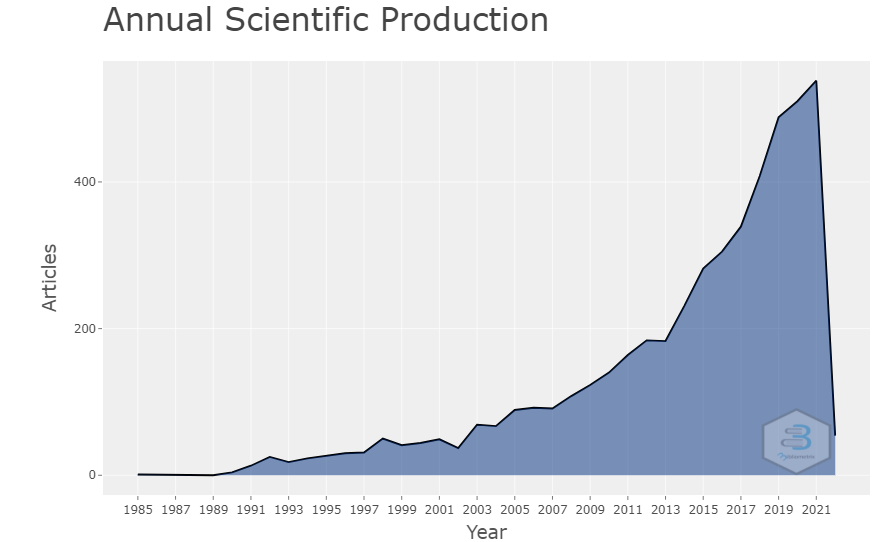
\includegraphics[width=1\textwidth]{experiments/KvotheKS/PesqBibliogr/AlgoritmosSimulacaoOptica-Dinamica/WoS-20220202/Dataset/Annual_Scientific.png}
    \caption{Produção anual científica}
    \label{fig:KvotheKS:Annual_Scientific}
\end{figure}
\subsection{Interpretação do crescimento}
    Com o avanço dos computadores e uma disponibilidade maior de recursos científicos como um todo, vários temas acabam ganhando força por fatores variados. No caso do meu \emph{dataset}, os estudos vão de análise topológica para robôs a estudo de aerodinâmica para aviões, e no fim acabam em simulações de iluminação.
\subsection{\emph{Clustering Network}}
    Como meio de demonstrar o quão "compacto" estão os resultados do \emph{dataset}, podemos utilizar uma \emph{Clustering Network}, que mostra em, em forma de grafo, quais estudos estão relacionados entre si, e qual peso de cada um.  
\begin{figure}[H]
    \centering
    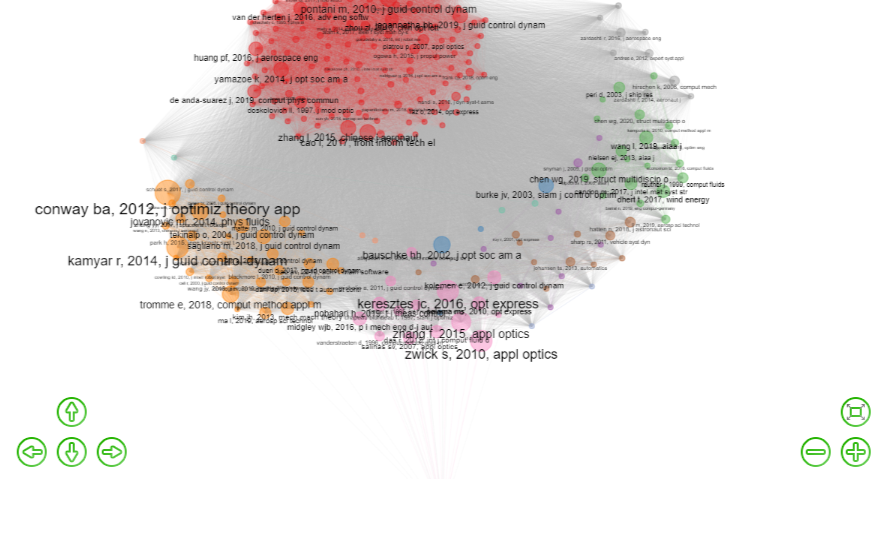
\includegraphics[width=1\textwidth]{experiments/KvotheKS/PesqBibliogr/AlgoritmosSimulacaoOptica-Dinamica/WoS-20220202/Dataset/Cluster_network.png}
    \caption{Grafo de citações}
    \label{fig:KvotheKS:Cluster_}
\end{figure}
\subsection{Interpretação da rede}
    Analisando a figura \ref{fig:KvotheKS:Cluster_}, podemos ver o quão inter-relacionados os artigos estão. Isso é um resultado óbvio do refinamento de dados feito anteriormente. Também mostra que alguns tópicos, como hidrodinâmica, aparecem em maior peso, por causa das revistas em qual artigos foram publicados. 
\subsection{\emph{Three-Field Plot}}
    Já foi demonstrado um dos \emph{Sankey diagrams} anteriormente \ref{fig:KvotheKS:Final_Data_Set}, onde o resultado mais interessante são as palavras-chave a direita, que mostram realmente quais são os tópicos mais abordados no \emph{dataset}. Porém alguns dados interessantes não foram abordados.
    
\begin{figure}[H]
    \centering
    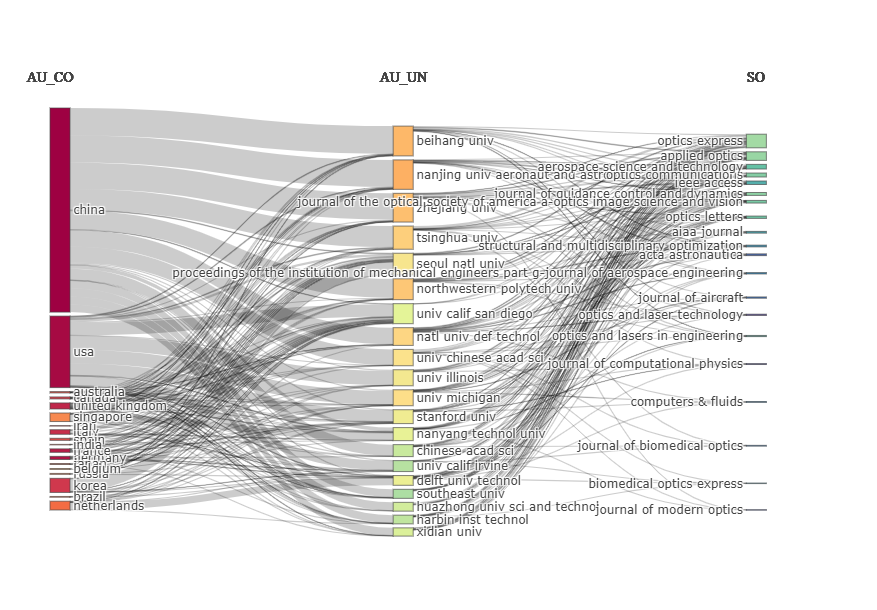
\includegraphics[width=1.1\textwidth]{experiments/KvotheKS/PesqBibliogr/AlgoritmosSimulacaoOptica-Dinamica/WoS-20220202/Dataset/AU_CO_AU_UN_SO.png}
    \caption{Afiliações, revistas e países}
    \label{fig:KvotheKS:SankeyCountry}
\end{figure}
\subsection{Considerações do peso dos países}
    Os dados interessantes da figura \ref{fig:KvotheKS:SankeyCountry} se dão nos países e universidades. Mais da metade dos artigos são chineses, porém não só há uma diversidade grande de universidades chinesas, mas também há uma falta de diferença entre as estado-unidenses, por onde artigos de vários países acabam passando.
\section{Análise final dos Dados}

%\chapter{Análise Bibliográfica sobre Simulação de Big Data na economia, por Tong Zhou\label{chap:bibliometria:Tong00020}}


\section{Planejamento do estudo}

O Big Data estuda, analisa e trata de um conjunto de dados maior e mais complexo que as processadas em sistemas tradicionais. Isso permite a resolução de problemas que não eram possíveis anteriormente.
%O planejamento o  desenho do estudo deve descrever as motivações, questões de interesse, escopo, limitações e objetivos do trabalho.

%O planejamento do estudo deve motivar o tema escolhido e o interesse do autor.

%No caso do meu trabalho, as perguntas que o nortearam foram:
%\begin{itemize}
%    \item Qual a base de conhecimentos científicos produzida em torno do tema simulação multiagente voltada à compreensão de fenômenos sociais, com ênfase em métodos experimentais? 
%    \item Como a simulação multiagente tem sido usada para compreender fenômenos sociais, com ênfase em métodos experimentais? 
%    \item Quais os principais termos e conceitos ligados à frente de pesquisa no tema simulação multiagente de fenômenos sociais, com ênfase em métodos experimentais? 
%    \item Qual a estrutura social da comunidade, se é que existe, que pesquisa sobre o tema simulação multiagente de fenômenos sociais, com ênfase em métodos experimentais?
%\end{itemize}

\begin{itemize}
    \item 
\end{itemize}


\subsection{O que já existe de pesquisa bibliométrica sobre esse tema?}


\subsection{Uso do Bibliometrix e Biblioshiny}

A pesquisa bibliométrica foi realizada com o uso do RStudio, foram usados o pacote \textit{Bibliometrix} e o aplicativo \textit{Biblioshiny} a partir do que foi apresentado em aula, como mostrado na figura ~\ref{fig:bibliometrix:workflow}. Através do acesso café do portal Periódicos CAPES, foi utilizada a \textit{Web of Science} para extrair os artigos usados na pesquisa.


\subsection{Limitações} 

Nesta tarefa foram feitas duas buscas na base de dados WoS, pois na primeira, o número de artigos não foi suficiente para gerar gráficos apresentáveis.


\section{Coleta de dados}

A coleta de dados feita usando o Web Of Science (WoS) no dia 03 de fevereiro de 2022, acessado por meio do Portal de Periódicos da CAPES. Foram feitas buscas nas coleções \textbf{Science  Citation  Index  Expanded (SCI -EXPANDED)}, \textbf{Social Sciences  Citation  Index (SSCI)}, \textbf{Conference Proceedings Citation Index-Science (CPI-S)} e \textbf{Emerging Sources Citation Index(ESCI)}. Foram colocados na pesquisa, artigos de 2010 a 2022. Foram encontrados 1265 artigos.

\subsection{Query de Busca}

Foi usada a query de busca abaixo: 

big data and economy (experimental  or  numeric* or  statist* or  hypothes* or  empiric* or  inferen * social  or  society  or  behavi *)

\subsubsection{Explicação para os termos de busca usados}


\subsection{Registros recuperados}

Os 1.265 registros obtidos como resultado da busca encontram-se em \url{https://github.com/jhcf/Comput-Experim-20212/experiments/Tong00020/PesqBibliogr/SimulacaoMultiagente/WoS-20220203/1265records.txt}

Foram utilizadas as opções \textit{Exportar registros para arquivo de texto sem formatação} e \textit{export full record / Gravar Conteúdo: Seleção personalizada, com todos os 29 campos disponíveis, inclusive referências citadas} no WoS, para que as citações também fosse usadas em análises da citações (estrutura intelectual do conhecimento). Os 1.265 registros foram recuperados em nove blocos de até 1.000 registros por vez (1-1000, 1001-1265).

\section{Análise dos dados}



\subsection{Filtragem de registros}

Sobrou 1.168 artigos ao colocar apenas "ARTICLE" como tipo de documento com o uso filtro do biblioshiny.



\subsection{Análise descritiva do %\textit{dataset} 
MASSA@Tong00020}

As informações mais gerais sobre o \textit{dataset} MASSA@Tong0020 são as seguintes:
\begin{description}
    \item[\textit{Timespan}] Os artigos da busca foram publicados a partir de 2010.
    \item [\textit{Sources (Journals, Books, etc)}] São 719 fontes publicaram os documentos no \dataset\. Em média, cada \textit{scientific journal} publicou $1.168/719=1,62$ artigos.%%%
     \item [\textit{Average years from publication}] A média do tempo de publicação dos artigos no dataset é de 3.25 anos.
     \item [\textit{Average citations per documents}] Cada artigo no dataset foi citado, em média 16.79 vezes.
     \item [\textit{Average citations per year per doc}] Após publicado, cada um dos 1.168 artigos do dataset foi citado 3.421 vezes por ano, em média.
    \item [\textit{References}] O dataset contém 61.413 referências citada.
    \item [\textit{Keywords Plus (ID)}] 2.857 distintas palavras-chave do tipo Keywords Plus (ID).
    \item [\textit{Author's Keywords (DE)}] 4.420 distintas palavras-chave indicadas pelos autores foram encontradas no \textit{dataset}.
     \item [\textit{Authors}] 10.181 nomes distintos de autores foram encontrados no \textit{dataset}.
    \item [\textit{Author Appearances}] Os 10.181 distintos (nomes de) autores foram encontrados 13.591 vezes, como autores de artigos.
    \item [\textit{Authors of single-authored documents}] Dentre os 10.181 distintos (nomes de) autores encontrados, 167 deles editaram artigos individualmente, isso é, sem co-autores.
    \item [\textit{Authors of multi-authored documents}] Dentre os 10.181 distintos (nomes de) autores encontrados, 10.014 deles editaram artigos com um ou mais co-autores"
    \item [\textit{Single-authored documents}] Dentre os 1.168 documentos presentes no \dataset\, 173 foram escritos por um único autor, e os 995 restantes foram elaborados em co-autoria.
    \item [\textit{Documents per Author}] Dentre os 10.181 distintos (nomes de) autores, cada um publicou em média 0,115 artigos.
    \item [\textit{Authors per Document}] Cada um dos 1.168 documentos presentes no \textit{dataset}  foi autorado com 8.72 autores em média ($10.181 / 1.168 = 8.72$).
    \item [\textit{Co-Authors per Documents}] As 13.591 aparições de (nomes de) autores (``Author Appearances''), sem distribuem, em média 11.6 vezes para os 1.168 documentos do \textit{dataset}.
    \item [\textit{Collaboration Index}] Os 10.181 (nomes de) autores que editaram artigos com um ou mais co-autores, colaboraram em media 10.1 vezes para editar os 1.168 artigos elaborados em co-autoria, gerando, assim, um índice de colaboração 10.1. 
    
\end{description}

     
\subsection{Evolução da Produção Científica}
A figura 
     
\subsubsection{Interpretação do Crescimento}

\subsection{Evolução das Citações}
A figura

\subsubsection{Interpretação da figura}
A figura

\subsection{\textit{Three-Field Plots (Sankey diagram)}}

\subsubsection{Interpretação da figura}
A figura

\subsection{Autores mais relevantes}
Apresentamos a seguir comentários sobre os autores mais citados nos trabalhos.

\subsection{Análises Bibliométricas: Fontes de Informação}

\subsection{Análises Bibliométricas: Autores}

\subsection{Análises Bibliométricas: Documentos}

\chapter{Análise Bibliográfica sobre Sistemas de Informação em transporte ...\label{chap:bibliometria:MoustacheGolem}}


%% Keywords usadas: (graphic processing unit or GPU) and (lighting or light or shadow*)

\chapter{Análise Bibliográfica sobre Graphics Processing Unit, por Gustavo Tomás}

\section{Planejamento do estudo}

O objetivo do trabalho é analisar o impacto e popularização das tecnologias utilizadas pelas GPUs (Graphic Processing Units) no processamento e simulação da luz. Para isso, foram utilizadas as ferramentas Bibliometrix e Biblioshiny. Algumas perguntas para basear a pesquisa são:

\begin{itemize}
    \item Como se deu o crescimento das pesquisas sobre GPUs com o passar dos anos?
    \item Quais autores possuem o maior impacto nesses campos de pesquisa?
\end{itemize}

\subsection{Limitações} O exercício relatado foi feito em cerca de uma semana, entre os dias 02 e 10 de fevereiro de 2022 e a base de dados utilizada foi Web Of Science (WoS).

\section{Coleta de dados}

A coleta de dados foi feita usando o WoS no dia 04/02/2022, por meio do Portal de Periódicos da CAPES. Foram feitas buscas nas coleções Science Citation Index Expanded (SCI-EXPANDED) e Social Sciences Citation Index (SSCI), mas com o foco em registros relativos a área de ciências naturais e exatas. A busca utilizada foi a seguinte:

\begin{verbatim}
(graphic processing unit or GPU) 
and
(lighting or light or shadow*)
\end{verbatim}

Essa busca consiste em dois termos, sendo que o primeiro é composto pela GPU (por extenso ou pela sigla) e o segundo pelas palavras luz ou iluminação ou sombra(s). Dessa forma, foram encontrados 1311 registros, sendo que nesse trabalho foram utilizados os primeiros 1000 registros. Esse dataset doravante será chamado de db\_GPU.

\section{Análise dos dados}

\subsection{Filtragem de registros}
Antes da análise, foram aplicados filtros aos registros, de forma que apenas registros do tipo \textit{article}, de qualquer ano e com qualquer número de citações, fossem analisados. O resultado consiste em 850/1000 registros originais.

\subsection{Análise descritiva do dataset}

As informações mais gerais sobre o \textit{dataset} são as seguintes:
\begin{description}
    \item  [\textit{Timespan}] Os artigos analisados foram publicados entre os anos de 1992 e 2022.
    \item  [\textit{Sources}] O dataset é composto por 360 fontes diferentes (dentre artigos, livros e outros).
    \item 
    [\textit{Average years from publication}] A média do tempo de publicação é de 6 anos.
    \item 
    [\textit{Average citations per document}] Cada artigo no dataset foi citado em média 18.55 vezes.
    \item 
    [\textit{References}] O dataset contém 27463 referências citadas.
\end{description}

\subsection{Evolução da Produção Científica}

O gráfico em \ref{fig:gpu-prod-cient} apresenta a evolução da produção científica, mostrando uma forte tendência de crescimento a partir de 2007.

\begin{figure}[ht]
    \centering
    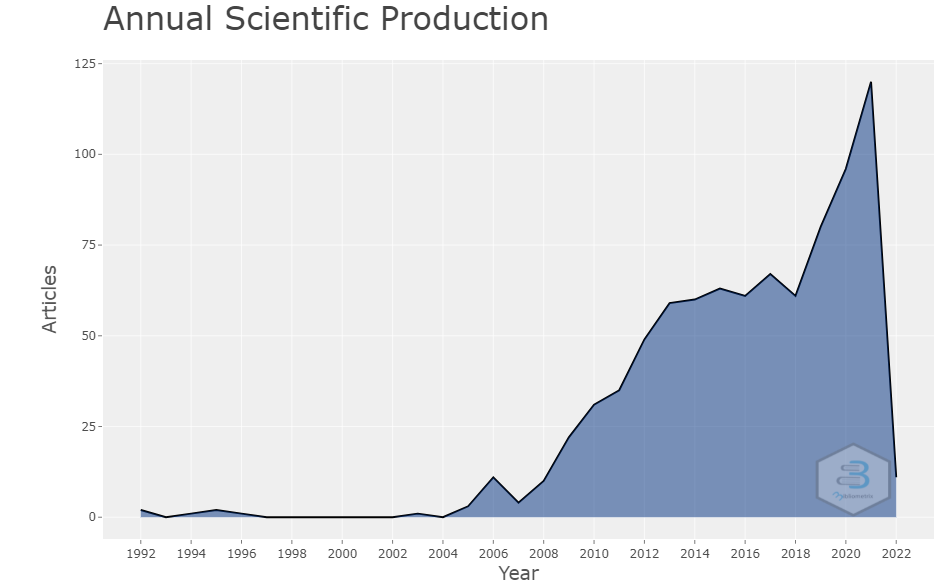
\includegraphics[width=12cm]{experiments/gustavo-tomas/AnaliseBibliometrica/GPUs/Graficos/gpu-prod-cient.png}
    \caption{Evolução da produção científica presente no \textit{db\_GPU}}
    \label{fig:gpu-prod-cient}
\end{figure}

O gráfico mostra um enorme crescimento na área, com destaque ao ano de 2021 com 120 documentos produzidos, um crescimento de 25\% em relação ao ano de 2020.

Nos anos de 2019-2021, em particular, foram introduzidas novas placas de vídeo no mercado, com poder computacional bem maior que as anteriores (é possível comparar as placas 1080 com as gerações 2080 e 3080 e perceber um aumento substancial de qualidade).

\subsection{Evolução das Citações}

A figura em \ref{fig:gpu-citation-year} mostra o número de citações médias feitas por ano. Nota-se uma grande quantidade de citações no ano de 2007, provavelmente devido a um artigo muito citado por outros autores. Nota-se também o que em uma faixa de 20 anos (1992-2021) o número de citações por ano aumentou de 0.2 para 1.0, um aumento de 5 vezes.

\begin{figure}[ht]
    \centering
    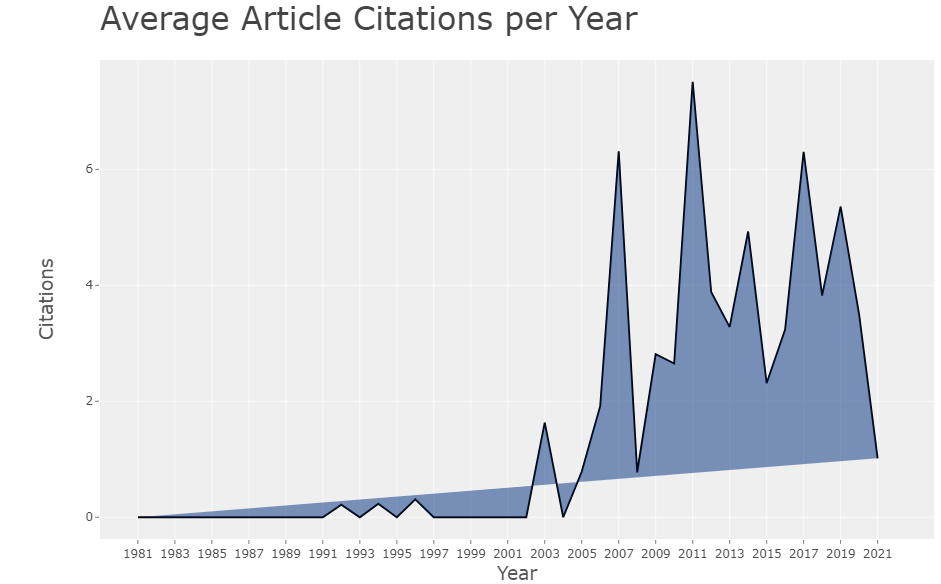
\includegraphics[width=12cm]{experiments/gustavo-tomas/AnaliseBibliometrica/GPUs/Graficos/gpu-citation-year.png}
    \caption{Evolução das citações por ano no \textit{db\_GPU}}
    \label{fig:gpu-citation-year}
\end{figure}

\subsection{\textit{Gráfico de três campos}}

O gráfico em \ref{fig:gpu-three-field} mostra um gráfico de três campos feitos com os dados acerca das referências, autores e palavras-chaves mais relevantes.

\begin{figure}[ht]
    \centering
    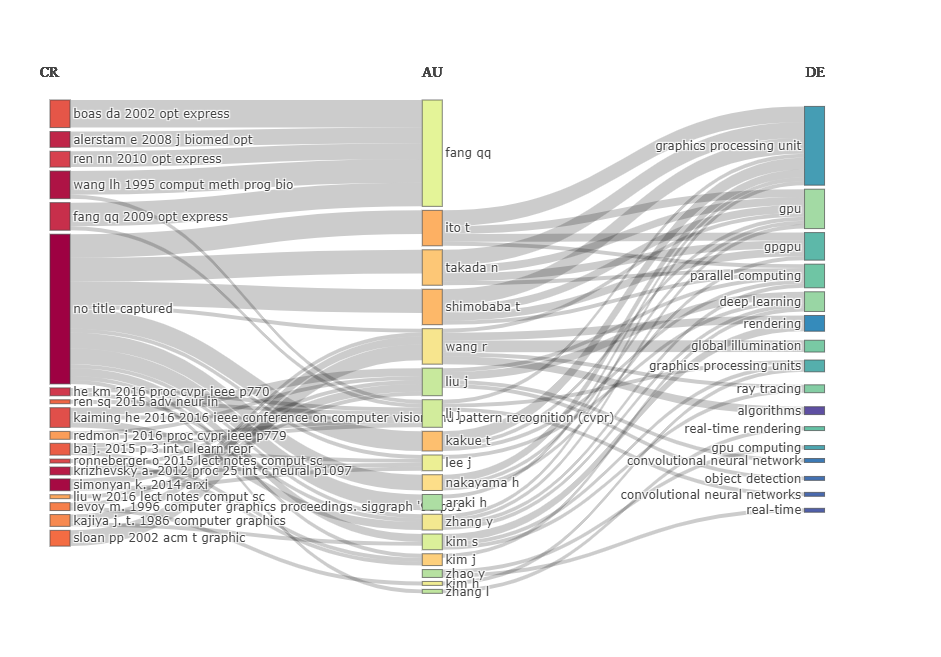
\includegraphics[width=12cm]{experiments/gustavo-tomas/AnaliseBibliometrica/GPUs/Graficos/gpu-three-field.png}
    \caption{Gráfico de três campos analisando palavras-chave no \textit{db\_GPU}}
    \label{fig:gpu-three-field}
\end{figure}

Observando as palavras-chaves, é possível perceber que termos como iluminação, processamento em paralelo e \textit{ray tracing} são expressões relevantes no contexto de GPUs.

Em particular, a técnica de \textit{Ray Tracing} foi otimizada nos últimos anos, de forma que é possível aplicá-la em simulações em tempo real (que antes não era possível devido ao alto custo computacional).

Observando os autores é possível perceber que a maior parte é de origem asiática e que esses autores utilizam principalmente \textit{masuda n 2006 opt express} como referência.

Essa publicação em específico relata avanços feitos na redução do custo computacional para geração de hologramas (objetos tridimensionais) em ambientes computacionais.

\subsection{Refinamento da coleta de dados}

O gráfico em \ref{fig:gpu-co-occur} mostra a rede de co-ocorrências de palavras-chave no \textit{db\_GPU}. Dentro os termos é possível perceber que os assuntos tratados são relevantes ao tópico de GPUs, com destaque ao campo em verde que separa assuntos relativos a dispersão de luz em meios turbulentos (\textit{turbid media}).

\begin{figure}[ht]
    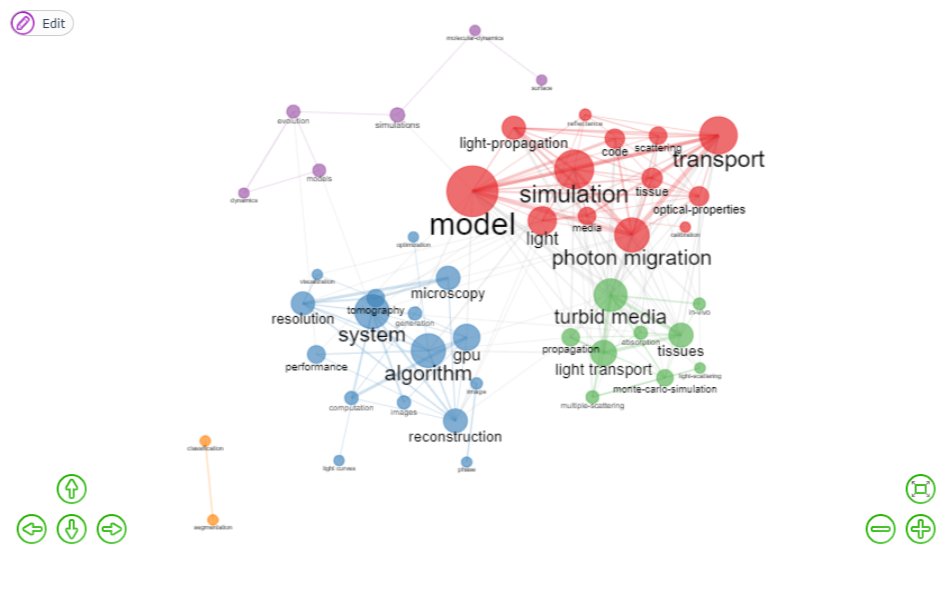
\includegraphics[width=12cm]{experiments/gustavo-tomas/AnaliseBibliometrica/GPUs/Graficos/gpu-co-ocurr.png}
    \caption{Rede de co-ocorrências de palavras-chave no \textit{db\_GPU}}
    \label{fig:gpu-co-occur}
\end{figure}

Esses tópicos são de especial interesse ao tópico de simulação de luz, pois essa simulação se dá por meio de aproximações ao mundo real (modelos físicos e fórmulas matemáticas). Um modelo eficiente consegue reter a essência dos fenômenos reais, de modo que é possível realizar uma simulação realista com uma capacidade computacional não tão elevada.

Softwares de animação (como blender) e de simulação possuem \textit{engines} que simulam fenômenos físicos, tais como corpos sólidos, emissores, índice de refração de materiais e reflexo da luz. Em especial, a \textbf{simulação de Monte Carlo} permite que uma amostra aleatória de possíveis caminhos de luz convirjam para uma solução correta, tornando esse método um dos métodos físicos mais precisos existentes.


\chapter{Análise Bibliográfica sobre Deepfakes, por Ítalo Eduardo Dias Frota\label{chap:bibliometria:titofrota}}

\section{Planejamento do estudo}

\textit{Deepfake}, uma junção de "\textit{deep learning}" e "\textit{fake}", se trata de técnicas de síntese de sons e imagens humanas baseadas em inteligência artificial. Com o avanço no desenvolvimento de algoritmos de \textit{deep learning}, é notório o crescimento na quantidade de tais conteúdos falsos publicados na internet.

Atualmente, o fenômeno das \textit{fake news} é amplamente discutido, o que abre espaço para debates em torno da produção de materiais falsos utilizando essa tecnologia.

O potencial das implicações sociais e políticas de tais materiais é extenso, podendo causar danos reais as vítimas de difamação política ou até mesmo "pornografia de vingança". Mas embora hajam debates éticos a respeito da tecnologia, os \textit{deepfakes} podem gerar avanços interessantes para as artes e cinema. 

Partindo dos pontos acima, as questões que nortearam a pesquisa foram:
\begin{itemize}
    \item Quais são as técnicas mais utilizadas na produção dos conteúdos?
    \item Quais são os impactos dos \textit{deepfakes}?
    \item Já existem métodos eficazes na detecção de \textit{deepfakes}? 
    \item Quais são as posições éticas presentes na comunidade de \textit{deepfakes}?
\end{itemize}

\subsection{Uso do Bibliometrix e Biblioshiny}
Serão usadas a ferramenta e o \textit{workflow} proposto pelos autores do pacote Bibliometrix, conforme indica a figura ~\ref{fig:bibliometrix:workflow}.

\subsection{Limitações} O exercício relatado foi feito em 8 horas, utilizando a base de dados Web of Science (WoS)


\section{Coleta de dados\label{MASSA:coleta}}

A coleta de dados feita usando a base Web of Science (WoS) no dia 05 de janeiro de 2022, acessado por meio do Portal de Periódicos da CAPES.

As buscas formam feitas nas coleções \textbf{Science  Citation  Index  Expanded (SCI -EXPANDED)} e \textbf{Social  Sciences  Citation  Index (SSCI)}, que contém registros relativos a vários campos do conhecimento, no qual o SCI-EXPANDED foca mais na área das ciências exatas e naturais, enquanto que o SSCI indexa artigos da área das ciências sociais. Observe que os artigos nessas duas coleções são indexados desde 1945. 

Foi usada a \textit{query} de busca ilustrada na listagem:

\lstinputlisting[numbers=left,basicstyle=\normalsize\ttfamily,caption={Query de busca sobre Deepfakes.}]
{experiments/titofrota/PesquisaBibliometrica/Deepfakes/query.txt}

\subsection{Explicação para os termos de busca usados\label{sec:titofrota:query}}

A busca utilizou cláusulas que retornassem registros relacionados a \textit{deepfakes} nos formatos visuais e auditivos. Evitando os registros que tratassem exclusivamente sobre \textit{fake news}, que não são o principal tópico da análise. Os termos podem aparecer no título, no \textit{abstract} e/ou nas \textit{keywords}. 

Os termos \texttt{deep}, \texttt{fake}, \texttt{speech}, \texttt{deepfake} buscam os resultados sobre \textit{deepfakes} e discursos falsos. O termo \texttt{news} é utilizado para excluir os resultados que tratavam sobre a detecção de \textit{fake news} através de algoritmos de \textit{deep learning}.

Foram obtidos 1.033 registros com a \textit{query} utilizada. Na exportação, foi utilizado o formato de arquivo de texto sem formatação, com os 29 campos disponíveis.

\section{Análise dos dados}

\subsection{Filtragem de registros}

Para a filtragem, removemos registros indesejados. O objetivo é obter apenas os artigos (supondo que o conhecimento de maior qualidade a respeito do tema está nas revistas, afinal é o método padrão de publicação científica), excluindo críticas, prévias, cartas e etc. Após a aplicação do filtro, 537 registros foram mantidos no \textit{dataset} que servirá como objeto da análise.

\subsection{Análise descritiva do \textit{dataset} }

A seguir, é feita uma análise bibliométrica descritiva do \textit{dataset} utilizando a função \texttt{biblioAnalysis} do Bibliometrix, que realiza diversos cálculos para levantar as taxas apresentadas.

As informações mais gerais sobre o \textit{dataset} são as seguintes:
\begin{description}
    \item [\textit{Timespan}] Os artigos filtrados foram publicados entre 1960 e 2022, o que indica que ainda há algum artigo não relacionado ao tema, que é relativamente recente.
    \item [\textit{Sources (Journals, Books, etc)}] São 340 fontes de informação que publicaram os artigos recuperados no \textit{dataset}. Logo, a média de publicações por \textit{scientific journal} é de $1.033/537=1,9$ artigos.
    \item [\textit{Average years from publication}] A média do tempo de publicação dos artigos no \textit{dataset} é de 3,59 anos.
    \item [\textit{Average citations per documents}] Cada artigo no \textit{dataset} foi citado, em média 13,63 vezes.
    \item [\textit{Average citations per year per doc}] Após publicado, cada um dos artigos foi citado, em média, 2,104 vezes por ano.
    \item [\textit{References}] O \textit{dataset} contém 20.312 referências citadas.
    \item [\textit{Keywords Plus (ID)}] 907 distintas palavras-chave do tipo Keywords Plus (ID) foram encontradas no \textit{dataset}.
    \item [\textit{Author's Keywords (DE)}] 1863 distintas palavras-chave indicadas pelos autores foram encontradas no \textit{dataset} .
    \item [\textit{Authors}] 2.063 distintos nomes de autores foram encontrados no \textit{dataset} .
    \item [\textit{Author Appearances}] Os 2.063 distintos (nomes de) autores foram encontrados 2.297 vezes, como autores de artigos.
    \item [\textit{Authors of single-authored documents}] Dentre os 2.063 distintos (nomes de) autores encontrados, 79 deles editaram artigos individualmente, isso é, sem co-autores.
    \item [\textit{Authors of multi-authored documents}] Dentre os 2.063 distintos (nomes de) autores encontrados, 1.984 deles editaram artigos com um ou mais co-autores"
    \item [\textit{Single-authored documents}] Dentre os 1.033 documentos presentes no \textit{dataset}, 79 foram escritos por um único autor, e os restantes foram elaborados em co-autoria.
    \item [\textit{Documents per Author}] Dentre os 2.063 distintos (nomes de) autores, cada um publicou em média 0,26 artigos.
    \item [\textit{Authors per Document}] Cada um dos 1.033 documentos presentes no \textit{dataset} foi autorado com 3,84 autores em média.
    \item [\textit{Co-Authors per Documents}] As 2.297 aparições de (nomes de) autores (``Author Appearances''), sem distribuem, em média 4,28 vezes para os 537 documentos do \textit{dataset}.
    \item [\textit{Collaboration Index}] Os 1.984 (nomes de) autores que editaram artigos com um ou mais co-autores, colaboraram em media 4.28 vezes para editar os 537 artigos elaborados em co-autoria, gerando, assim, um índice de colaboração 4,33. 
\end{description}

\subsection{Evolução da Produção Científica}

\begin{figure}
    \centering
    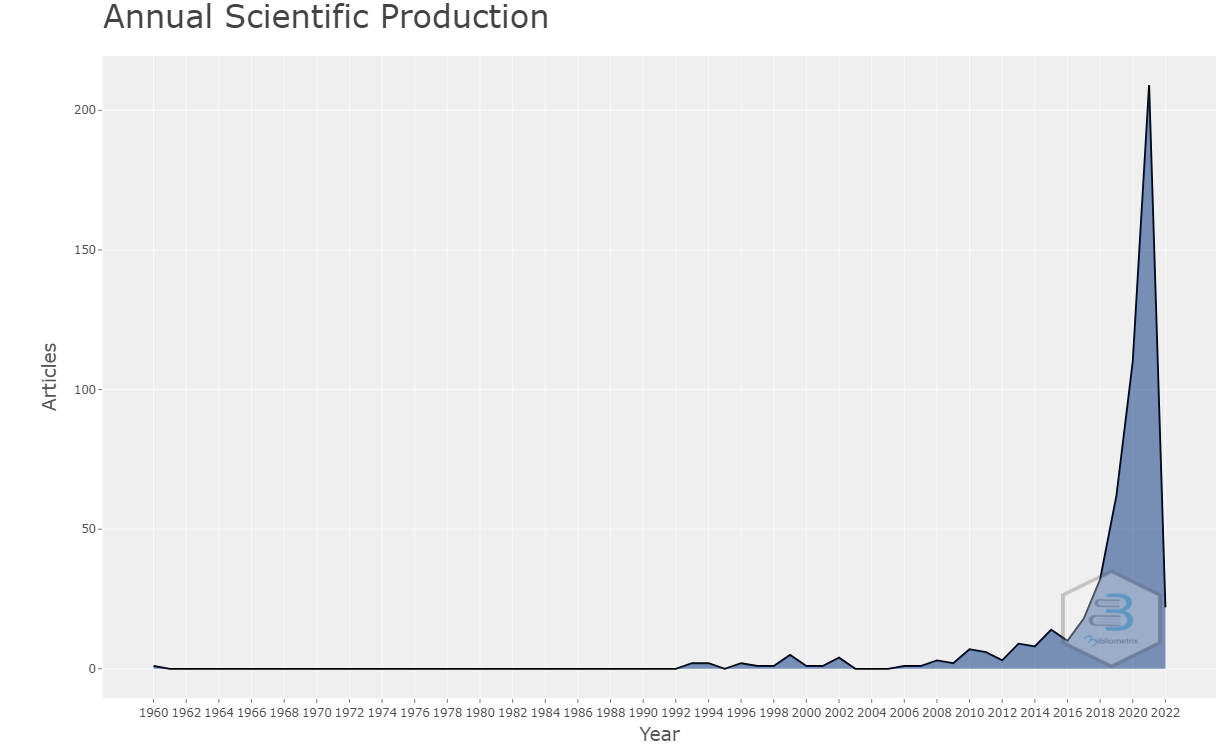
\includegraphics[width=1\textwidth]{experiments/titofrota/PesquisaBibliometrica/Deepfakes/annual-plot.png}
    \caption{Evolução da produção científica no \textit{dataset}}
    \label{fig:evol:anual:DEEPFAKES@titofrota}
\end{figure}

A figura \ref{fig:evol:anual:DEEPFAKES@titofrota} representa a evolução em produção científica mundial a respeito do tema, de acordo com o \textit{dataset}. Houve um crescimento a notável a partir do ano de 2020, atingindo o pico em 2021. 
É perceptível que no \textit{dataset} ainda há artigos não relacionados ao tema analisado.

O \textit{Annual Growth Rate} do \textit{dataset} é de 12,62\%, que é um valor alto comparado a média de crescimento da comunidade científica como um todo.

\subsection{Interpretação do Crescimento} a taxa de crescimento do \textit{dataset} demonstra que o tema tem chamado muita atenção nos últimos anos, provavelmente devido aos escândalos envolvendo pessoas públicas e os \textit{deepfakes}.

\subsection{Evolução das Citações}

\begin{figure}
    \centering
    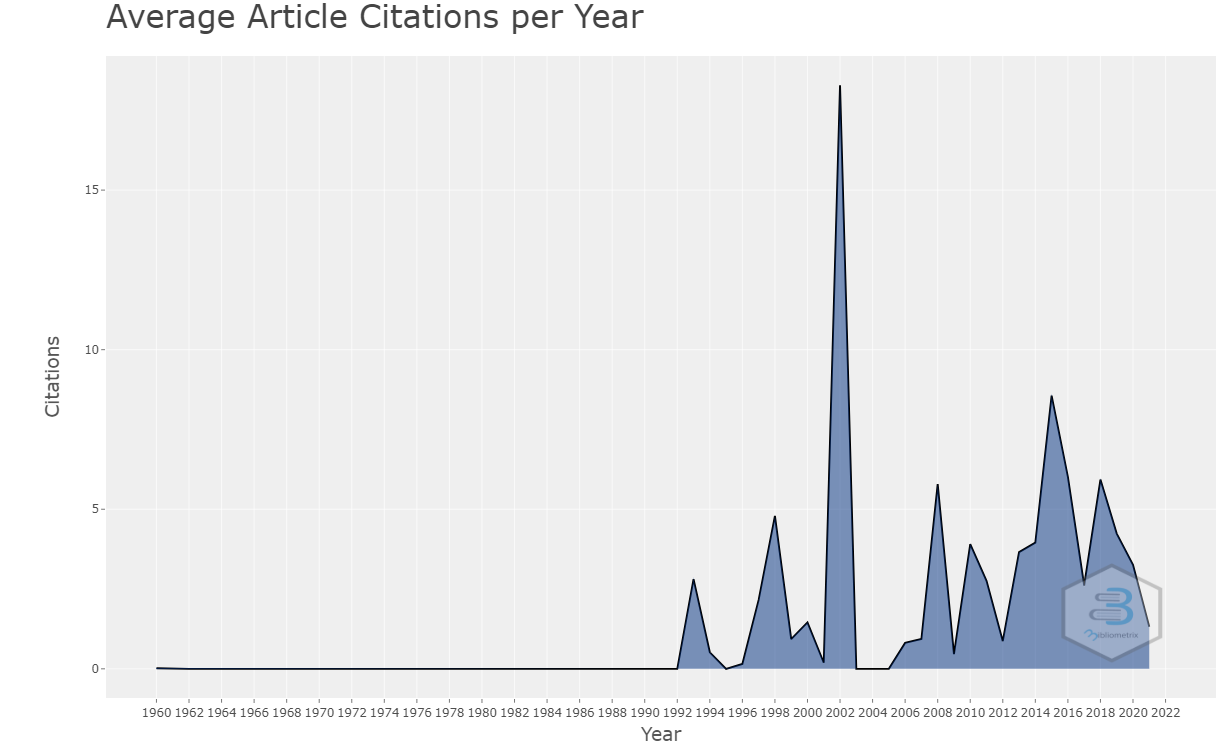
\includegraphics[angle=0,width=1\textwidth]{experiments/titofrota/PesquisaBibliometrica/Deepfakes/citations-year-plot.png}
    \caption{Evolução das citações ao \textit{dataset}.}
    \label{fig:evol:anual:citacoes:DEEPFAKES@titofrota}
\end{figure}

A figura \ref{fig:evol:anual:citacoes:DEEPFAKES@titofrota} apresenta a evolução da média de citações aos artigos do \textit{dataset}. Não há muita estabilidade na média anual de citações, até mesmo nos anos mais recentes.

\subsection{Interpretação das Citações}
Embora a taxa de crescimento de publicações anuais seja alta, ainda há instabilidade no que diz respeito a média de citações. Demonstrando que o tema ainda é um tanto prematuro, necessitando de mais atenção pelos cientistas.

\subsection{\textit{Three-Field Plots (Sankey diagram)}}

As \textit{Three-Field Plots (Sankey diagram)} (plotagens do tipo ``Três Campos'') correlacionam três conjuntos de atributos em busca das afinidades encontradas no \textit{dataset}. Assim, são demonstrados os principais fluxos entre diferentes conjuntos.

\begin{figure}
    \centering
    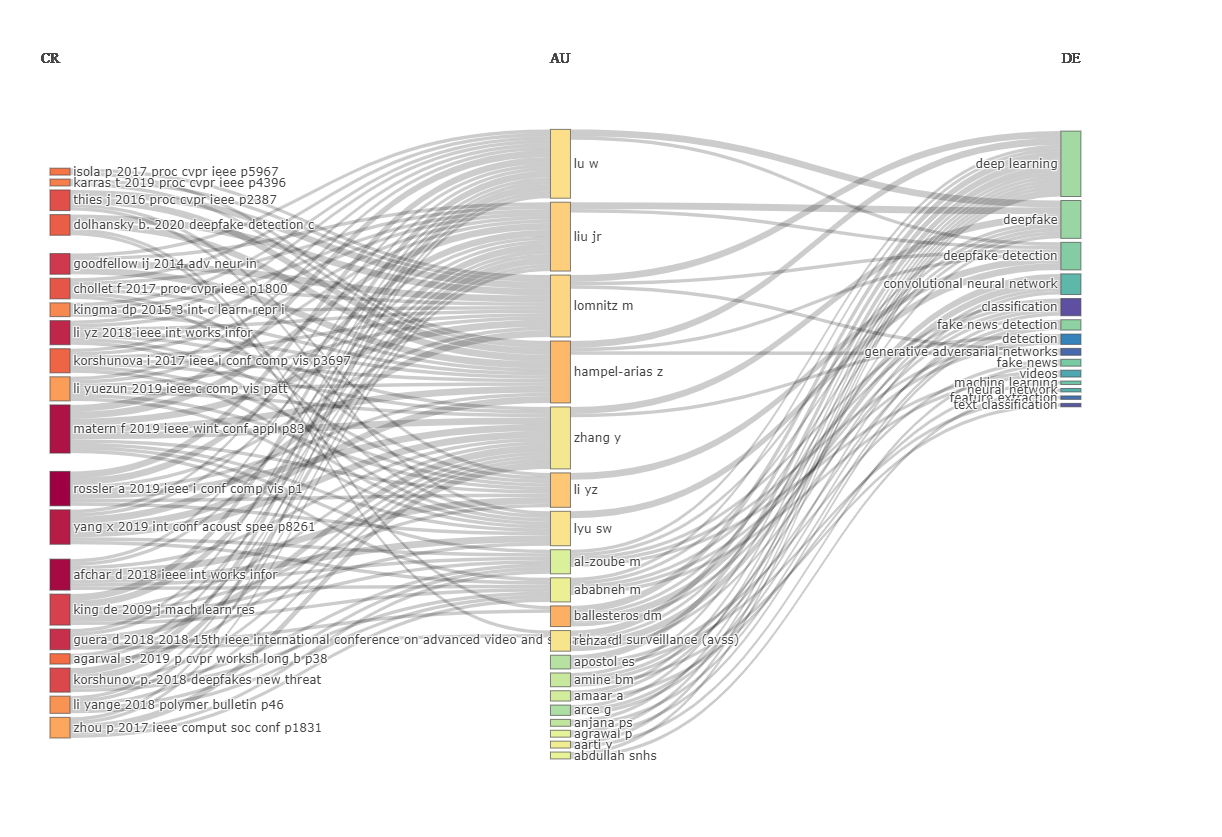
\includegraphics[width=1\textwidth]{experiments/titofrota/PesquisaBibliometrica/Deepfakes/ThreeFieldPlot.png}
    \caption{Plotagem ``Três Campos'' (Sankey plot) do \textit{dataset}: 20 Autores, Citações e 14 Palavras-Chave mais proeminentes.}
    \label{fig:DEEPFAKES@titofrota:ThreeFieldPlot}
\end{figure}

A figura \ref{fig:DEEPFAKES@titofrota:ThreeFieldPlot} apresenta a plotagem do tipo ``Três Campos'' realizada no \textit{dataset}, vinculando, ao centro, os 20 Autores mais proeminentes (AU), à esquerda, as 20 Citações mais frequentes (CR - Cited Records), e à direita, as 14 Palavras-Chave mais frequentes empregadas pelos autores.

\subsection{Interpretação da figura \ref{fig:DEEPFAKES@titofrota:ThreeFieldPlot}}
A maioria dos autores mais relevantes apresentados na plotagem são, aparentemente, de origem oriental, mais especificamente chinesa. Além disso, uma quantidade razoável dos artigos surgiram em universidades da China. O que sugere o avanço e a preocupação do oriente a respeito do tema analisado.

É possível observar nas palavras-chave que há bastante interesse na detecção de \textit{deepfakes}, apresentam-se os termos \textbf{deepfake detection}, \textbf{fake news detection} e \textbf{detection}. Os resultados sugerem que há interesse em remediar os impactos que os conteúdos criados através de algoritmos de \textit{deep learning} podem causar à sociedade.

\section{Refinamento da Coleta de Dados}

Após a análise do \textit{dataset}, foi possível notar que há a presença de artigos que não estão relacionados ao tema. A observação indica a necessidade de uma nova busca, visando a exclusão de artigos não relacionados ao desenvolvimento de \textit{deepfakes}.

Ao analisar a rede de co-ocorrência de palavras aplicada ao \textit{dataset}, foram identificadas algumas palavras no cluster que não correspondem ao assunto trabalhado. Assim, surgiu uma nova \textit{query} para levantar artigos mais apurados e relevantes.

\begin{figure}[htp]
    \centering
    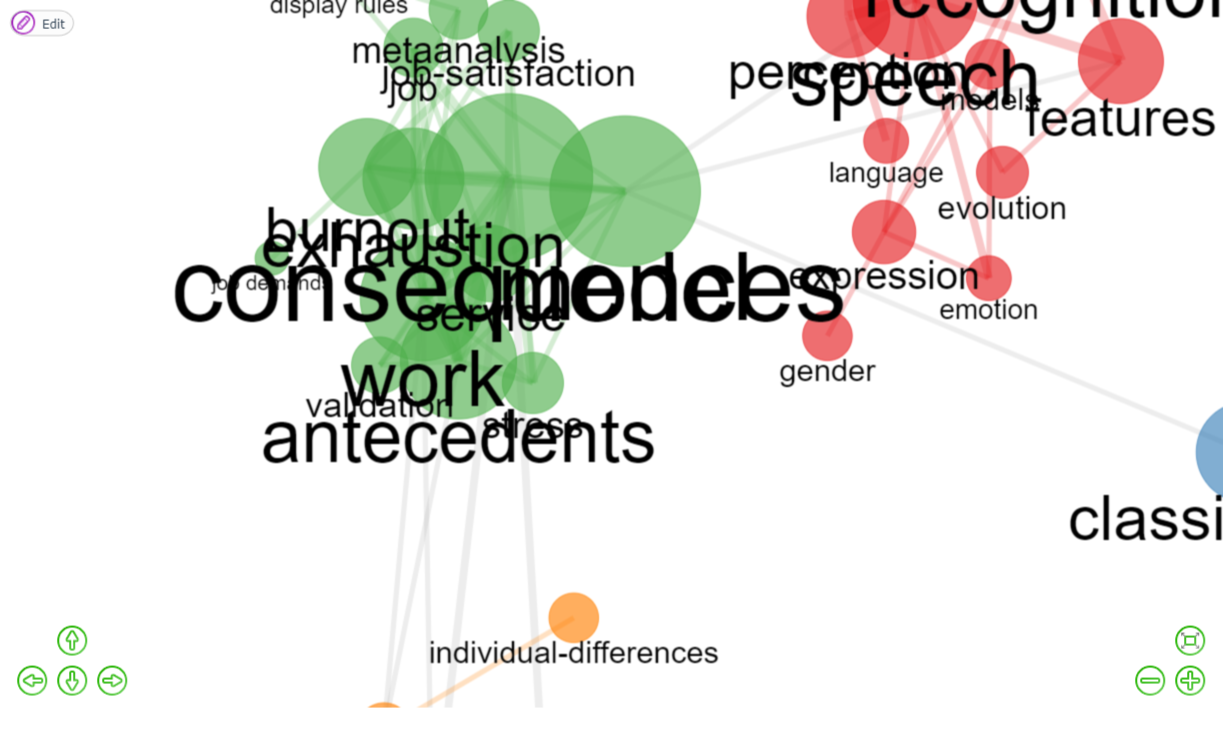
\includegraphics[width=0.6\textwidth]{experiments/titofrota/PesquisaBibliometrica/Deepfakes/co-ocurrence.png}
    \caption{Rede de co-ocorrência de palavras aplicada ao \textit{dataset}.}
    \label{fig:DEEPFAKES@titofrota:redecoocorrencia}
\end{figure}

A nova \textit{query} leva em conta novos termos e a busca foi feita nas publicações entre 2017 (quando o termo \textit{deepfake} surgiu) e 2022.

\lstinputlisting[numbers=left,basicstyle=\normalsize\ttfamily,caption={Query refinada de busca sobre Deepfakes.}]
{experiments/titofrota/PesquisaBibliometrica/Deepfakes/new-query.txt}


Além das justificativas para os termos usados entre as linhas 1 a 9, já descritas em \ref{MASSA:query},  justifica-se na listagem \ref{query20220203}, a inclusão da cláusula \textit{not (
 adsoption or molecular -dynamics or force -field
 or in -vitro or nanopartic* or in -vivo
 or aqueous -solution or protein or surface)}, entre as linhas 10 e 13 da \query, pois elas irão remover artigos não se enquadram no escopo da busca desejada, por usarem uma ou mais desses termos no título, resumo ou palavras-chave do artigo.
 
 Foram incluídas cláusulas como \textbf{deep-fake} e \textbf{face-swap*} com o intuito de encontrar mais conteúdos relacionados ao tema. Além disso, foram adicionadas novas cláusulas negadas para filtrar melhor os resultados, evitando que artigos médicos ou relacionados à outros temas façam parte do novo \textit{dataset}.
 
Usando a nova \textit{} de busca, foram recuperados 284 documentos. Sendo assim, aproximadamente 749 registros não se enquadravam na necessidade de busca.
Uma nova análise dos dados recuperados é apresentada a seguir.

\section{Nova Análise dos Dados}

\subsection{Nova filtragem de registros}

São aplicados dois filtros aos 284 documentos recuperados:
\begin{itemize}
    \item Remoção dos registros de documentos que não são artigos \textit{full paper}, isso é, artigos completos publicados em revistas;
    \item Remoção dos registros de artigos científicos que não fazem parte do \textit{core} da bibliografa, segundo a Lei de Bradford.
\end{itemize}

Após a filtragem, foram obtidos apenas 79 registros, que correspondem ao novo \textit{dataset}.
08
\subsection{Análise descritiva do \textit{dataset} refinado}

\begin{table}[]
    \centering
\csvautotabular[separator=semicolon
%,filter not strcmp={\csvcolii}{}
]{experiments/titofrota/PesquisaBibliometrica/Deepfakes/main-info.csv}
    \caption{Principais dados descritivos do dataset refinado.}
    \label{tab:DEEPFAKE:Main}
\end{table}

Logo, de acordo com a tabela \ref{tab:DEEPFAKE:Main}, é possível notar que entre 2017 e 2022 houveram 240 artigos publicados em 94 revistas diferentes.

\chapter{Análise Bibliográfica sobre Neurociência e Inteligência Artificial por Stefano Luppi Spósito\label{chap:bibliometria:kawaiistheno}}

\section{Planejamento do Estudo}

Atualmente, é fato que o ser humano está sempre conectado à tecnologia de alguma forma, seja pelo seu smartphone ou pelo seu computador pessoal. Também é um fato que, o ser humano sempre estará preso à tecnologia de seu tempo e, assim, podendo nunca desbravar as grandes revoluções que poderão acontecer no futuro.

Essa pesquisa tem como principal foco apresentar os possíveis desenvolvimentos da tecnologia, relacionados ao campo da neurociência ligada com a inteligência artificial. Sabemos hoje que ainda não é possível medir emoções, entretanto, valência e ativação emocional podem ser medidas facilmente.

Tendo em vista o que foi falado anteriormente, é possível apresentar algumas questões que motivam a criação desta análise:

\begin{itemize}
    \item Quais os impactos sobre o cálculo de emoções a Neurociência e Inteligência Artificial trarão no futuro?
    \item Quais benefícios para a sociedade seriam alcançados a partir da evolução dos estudos e conquistas nesse campo?
    \item Até que ponto podemos considerar o campo da Neurociência e Inteligência Artificial benéfico para a humanidade?
\end{itemize}

\subsection{O que já existe de pesquisa bibliométrica sobre esse tema?}

Atualmente, existem diversas pesquisas relacionadas a este tema. Algumas delas relacionadas ao uso da Neurociência em conjunto da Inteligência Artificial na política e sistemas judiciais. Além disso, pesquisas sobre a utilização dessas áreas para a simulação de funcionalidades do cérebro humano também estão sendo feitas.

\subsection{Uso do Bibliometrix e Biblioshiny}

Para a execução desta análise, foram utilizados o Biliometrix e Biblioshiny, que foram necessários para adquirir informações sobre as pesquisas feitas na área de Neurociência e Inteligência Artificial.

\subsection{Limitações}

O exercício foi feito em aproximadamente 3 dias consecutivos, onde o autor dedicou 2 horas em cada dia para poder realizar as pesquisas necessárias. A princípio, a pouca experiência com a linguagem R e o próprio Bibliometrix se provou ser uma grande dificuldade, mas eventualmente os objetivos foram concluídos graças as aulas e slides disponibilizados pelo professor da matéria.

\section{Coleta de Dados}

A coleta de dados feita usando o WoS no dia 06 de fevereiro de 2022, acessado por meio do Portal de Periódicos da CAPES.

Foram feitas pesquisas utilizando o termo \textbf{Neuroscience and Artificial Intelligence} para buscar resultados que condissessem com o tema desta análise.

\section{Análise dos Dados}

\subsection{Filtragem de registros}

Inicialmente, o \dataset\ apresentava 620 resultados, que continham prévias de artigos, livros, reviews de livros, entre outros. Para uma maior compreensão e visualização de resultados relevantes para esta análise, foram aplicados filtros que permitissem que o \dataset retornasse apenas artigos completos, visto que do ponto de vista do autor desta análise, artigos são mais confiáveis, se comparados com outras fontes. Após a aplicação dos filtros, foram retornados 349 resultados pelo \dataset 

\subsection{Análise descritiva do \dataset }

A análise bibliométrica descritiva faz uma descrição inicial do \dataset\  . Para explicação detalhada de como são calculadas as diversas taxas geradas pelo Bibliometrix veja a documentação do \textit{package} a partir da página \url{https://cran.r-project.org/web/packages/bibliometrix/index.html}. A análise bibliométrica descritiva é gerada pela função \texttt{biblioAnalysis}.

As informações mais gerais sobre o \dataset\ são as seguintes:
\begin{description}
    \item [\textit{Timespan}] Os artigos que atenderam aos critérios de busca e filtragem foram publicados a partir de 1988, até 2022. Ou seja, não foram encontrados registros entre 1945 e 1987.
    \item [\textit{Sources (Journals, Books, etc)}] São 235 fontes de informação que publicaram os documentos recuperados no \dataset\. Ou seja, em média, cada \textit{article} publicou $349/235=1,4$ artigos.
    \item [\textit{Average years from publication}] A média do tempo de publicação dos artigos no \dataset\ é de 5,38 anos.
    \item [\textit{Average citations per documents}] Cada artigo no \dataset\ foi citado, em média 14,25 vezes
    \item [\textit{Average citations per year per doc}] Após publicado, cada um dos 349 artigos do \dataset\   foram citados 2,463 vezes por ano, em média.
    \item [\textit{References}] O \dataset\ contém 21.506 referências citadas (tags CR).
    \item [\textit{Keywords Plus (ID)}] 872 distintas palavras-chave do tipo Keywords Plus (ID)\footnote{\textit{KeyWords Plus} são ``termos de índice gerados automaticamente a partir dos títulos de artigos citados. Os termos do KeyWords Plus devem aparecer mais de uma vez na bibliografia e são ordenados de frases com várias palavras a termos únicos. O KeyWords Plus aumenta o número de resultados tradicional de palavras-chave ou títulos.'' Fonte: \url{https://images.webofknowledge.com/WOKRS410B4/help/pt_BR/WOS/hp_full_record.html}} foram encontradas no \dataset\   . 
    \item [\textit{Author's Keywords (DE)}] 1.287 distintas palavras-chave indicadas pelos autores foram encontradas no \dataset\  .
    \item [\textit{Authors}] 1.116 distintos nomes de autores foram encontrados no \dataset\  \footnote{Um mesmo autor pode ter uma ou mais diferentes grafias no \dataset\  , e serão reconhecidos dois ou mais autores diferentes, embora de fato sejam apenas um. Isso significa que a quantidade de \textbf{nomes de autores} equivale à quantidade de \textbf{autores}. Adicionalmente, é possível que distintos autores sejam reconhecidos com o mesmo nome, isso é, que sejam homônimos. Ou seja, o \dataset\   em geral conterá erros de contagem na quantidade de autores reais.}.
    \item [\textit{Author Appearances}] Os 1.116 distintos (nomes de) autores foram encontrados 1.187 vezes, como autores de artigos.
    \item [\textit{Authors of single-authored documents}] Dentre os 1.116 distintos (nomes de) autores encontrados, 117 deles editaram artigos individualmente, isso é, sem co-autores.
    \item [\textit{Authors of multi-authored documents}] Dentre os 1.116 distintos (nomes de) autores encontrados, 999 deles editaram artigos com um ou mais co-autores"
    \item [\textit{Single-authored documents}] Dentre os 349 documentos presentes no \dataset\  , 123 foram escritos por um único autor, e os 226 restantes foram elaborados em co-autoria.
    \item [\textit{Documents per Author}] Dentre os 1.116 distintos (nomes de) autores, cada um publicou em média 0,313 artigos.
    \item [\textit{Authors per Document}] Cada um dos 349 documentos presentes no \dataset\  foram autorados com 3,2 autores em média ($1.116 / 349 = 3,19$).
    \item [\textit{Co-Authors per Documents}] As 1.187 aparições de (nomes de) autores (``Author Appearances''), se distribuem, em média 3.4 vezes para os 349 documentos do \dataset\ .
    \item [\textit{Collaboration Index}] Os 1.116 (nomes de) autores que editaram artigos com um ou mais co-autores, colaboraram em media 4.42 vezes para editar os 349 artigos elaborados em co-autoria.
\end{description}

\subsection{Evolução da Produção Científica}

\begin{figure}
    \centering
    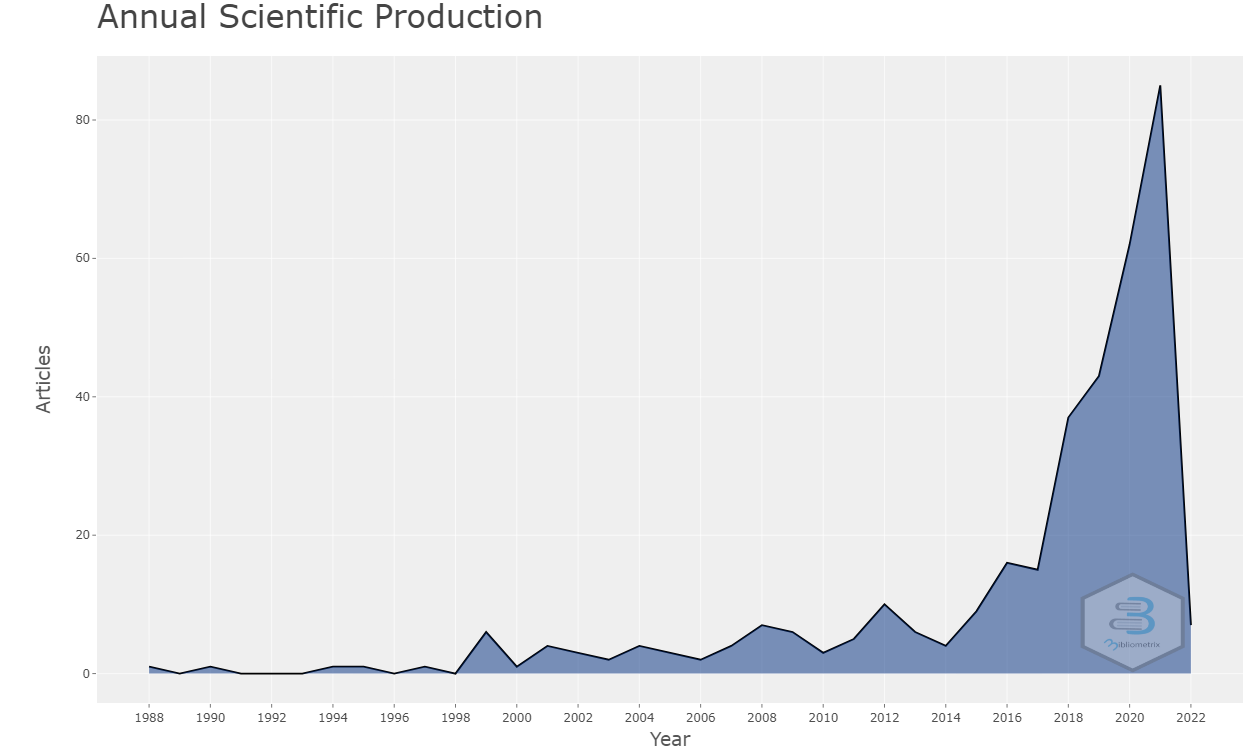
\includegraphics[width=1\textwidth]{experiments/KawaiiStheno/PesqBibliogr/NeurocienciaIIA/WoS-20220206/scientificProdution.png}
    \caption{Evolução da produção científica no \dataset\   kawaiistheno.}
    \label{fig:evol:anual:kawaiistheno}
\end{figure}

Observando a figura \ref{fig:evol:anual:kawaiistheno}, podemos perceber uma evolução gradativa na quantidade de artigos ao longo dos anos, tendo uma explosão de novos artigos a partir do ano de 2014.

\subsection{Evolução das Citações}

\begin{figure}
    \centering
    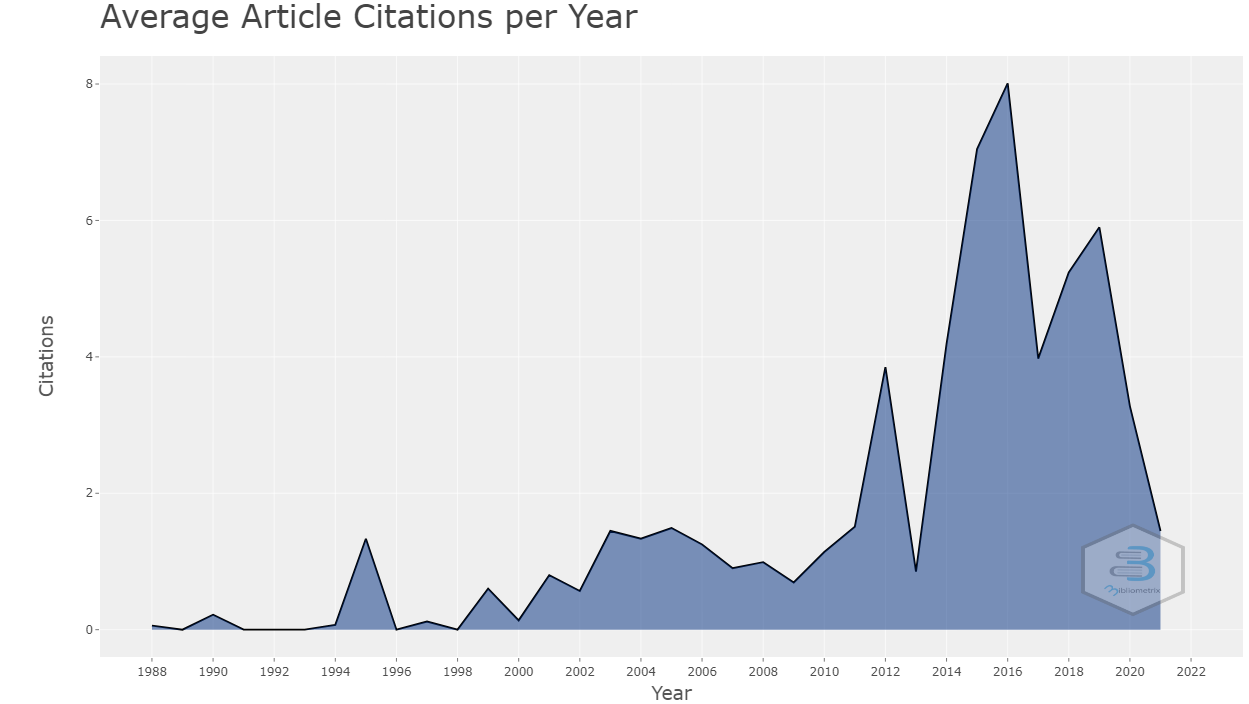
\includegraphics[width=1\textwidth]{experiments/KawaiiStheno/PesqBibliogr/NeurocienciaIIA/WoS-20220206/citationsYear.png}
    \caption{Evolução das citações ao \dataset\   kawaiistheno.}
    \label{fig:cit:anual:kawaiistheno}
\end{figure}

É possível observar em \ref{fig:evol:anual:kawaiistheno} que o número de citações começou a crescer lentamente a partir de 1998, sofrendo uma explosão neste crescimento em 2014. Se compararmos com a figura \ref{fig:evol:anual:kawaiistheno} podemos perceber que neste ano, a produção científica também teve um aumento considerável de artigos produzidos, indicando que 2014 foi um ano de expre

\subsection{Three-Field Plots (Sankey diagram)}

\chapter{Análise Bibliográfica sobre o Uso de Big Data na Política, por Enzo Nunes Leal Sampaio}

\section{Planejamento do estudo}
Política, do grego \textit{politikos} significa algo relacionado com grupos sociais que integram a Pólis \citep{wikipedia_politica_nodate}. Diante dessa definição podemos assumir que a política faz parte do dia a dia de todas as pessoas.

A partir desse pensamento foi questionado sobre a participação da computação nesse tema. Mais especificamente, como o Big Data pode influenciar na política.

Dessa forma, os questionamentos que norteam este estudo são:

\begin{itemize}
    \item Qual a base de conhecimento produzida sobre o tema de Uso de Big Data na Política?
    \item Como os partidos políticos usam o Big Data em suas campanhas?
    \item Como certos grupos políticos podem se beneficiam do uso de Big Data?
\end{itemize}

\subsection{Uso do Bibliometrix e Biblioshiny}

O Bibliometrix é uma biblioteca da linguagem R que permite a realização de análises quantitativas e estatística sobre publicações científicas.

O Biblioshiny é uma ferramenta do pacote Bibliometrix que contribui com aspectos visuais às funções executadas pela biblioteca.

A pesquisa bibliográfica sobre o tema já mencionado é feita usando, principalmente, essas duas ferramentas.

\subsection{Limitações}
O estudo foi feito em uma semana com trabalhos de duração de uma hora por dia e utilizando somente a base de dados Web of Science(WoS).

\section{Coleta de dados}
A coleta de dados foi feita a partir da base Web of Science no dia 3 de fevereiro de 2022, acessado pelo Portal de Periódicos da CAPES. As buscas foram feitas nas coleções Science Citation Index Expanded(SCI-EXPANDED) e Social Sciences Citation Index (SSCI) com foco nas categorias relacionadas às ciências exatas e foram obtidos 2540 registros. A pesquisa pode ser vista a seguir:

\lstinputlisting[numbers=left,basicstyle=\normalsize\ttfamily]{experiments/enzodevs2000/AnaliseBibliometrica/BigDataInPolicy/busca.tex}

\subsection{Explicações para os termos de busca usados}
Como o objetivo é buscar registros que relacionem \textbf{Big Data} e \textbf{Política} é feita uma conjunção entre duas cláusulas principais, sendo que, na primeira tem-se uma outra cláusula conjuntiva entre as palavras \textit{big} e \textit{data}. Já na segunda cláusula principal tem-se uma disjunção entre 4 cláusulas.

A primeira é uma disjunção entre \textit{politica} e \textit{parties}. A segunda é \textit{elections}. A terceira é uma disjunção entre \textit{party} e \textit{campaigns}. Essas três cláusulas são feitas tendo como objetivo obter registros que ajudem a responder o segundo questionamento feito na primeira seção deste texto.

Por fim, a última cláusula \textit{policy} busca associar todos os temas já relatados com política.

\chapter{Análise Bibliográfica sobre reconhecimento biométrico, por João Pedro Felix}

\section{Planejamento do estudo}
Do controle de acesso a um dispositivo celular até a autenticação de um eleitor para o uso da urna eletrônica, a biometria tem se mostrado uma das maneiras mais eficazes de garantir que alguém é de fato quem afirma ser.

Reconhecimento de digital, iris, palmar e facial são apenas algumas das maneiras mais comuns de se realizar essa identificação, que parte do princípio que, na prática, essas características podem ser consideradas únicas para cada pessoa.

Isso tudo me leva a questionar, por exemplo, os seguintes fatores:

\begin{enumerate}
    \item Quais são os conceitos mais relevantes relacionados com identificação biométrica?
    \item Quais são os métodos mais relevantes de reconhecimento biométrico?
    \item Quem são os autores mais relevantes e com quais tópicos mais específicos eles trabalham?
\end{enumerate}

\subsection{O que já existe de pesquisa bibliométrica sobre biometria?}

Um estudo bibliométrico sobre identificação biométrica a partir do movimento dos olhos foi proposto por \citet{brasil_eye_2020}, contudo, o objetivo lá apresentado é diferente daqui, uma vez que minha intenção é ter uma visão mais geral no assunto, justamente por ainda ter pouco conhecimento na área.

\subsection{Ferramentas Utilizadas}

A realização da pesquisa bibliométrica será realizada a partir da ferramenta RStudio, juntamente do pacote \textit{Bibliometrix} e do aplicativo \textit{Biblioshiny}. Os artigos que serão usados foram extraídos da base de dados \textit{Web of Science}.

\section{Coleta de Dados}

A coleta de dados foi realizada utilizando a base de dados Web of Science no dia 03/02/2022, acessada por meio do Portal de Periódicos da CAPES.

A busca foi feita utilizando as coleções Science Citation Index Expanded (SCI-Expanded)--1945-presente, Conference Proceedings Citation index - Science (CPCI-S)--1990-presente e Emergin Sources Citation Index (ESCI)--2017-presente.

\subsection{Busca e refinamento}
Inicialmente a busca realizada foi a apresentada em \ref{BIPA@DYosplayQueryBiometrics1}, que procurou por artigos que contivessem o seguinte tópico:


\lstinputlisting[numbers=left,basicstyle=\normalsize\ttfamily,caption={Pesquisa sobre biometria},label=BIPA@DYosplayQueryBiometrics1]
{experiments/DYosplay/PesquisaBibliometrica/Pesquisas/pesquisa1.txt}


A ideia inicial era encontrar artigos que tratassem de biometria e processamento de imagens, a intenção com isso era evitar em especial artigos mais focados na área de biologia por exemplo, ao priorizar os que tivessem relação direta com processamento de imagens.

Contudo, foram obtidos apenas cerca de 2000 resultados. Assim, uma nova busca foi realizada, como mostrado abaixo (em \ref{BIPA@DYosplayQueryBiometrics2}), que resultou em 5252 itens encontrados.

\lstinputlisting[numbers=left,basicstyle=\normalsize\ttfamily,caption={Pesquisa refinada sobre biometria},label=BIPA@DYosplayQueryBiometrics2]
{experiments/DYosplay/PesquisaBibliometrica/Pesquisas/pesquisa2.txt}

A melhora aconteceu ao incluir na busca os termos \textit{recognition}, que significa "reconhecimento", e \textit{verification}, que significa "verificação", como alternativa a \textit{processing} que significa "processamento", mas sem abrir mão de \textit{image}, que quer dizer "imagem". 

A ideia surgiu ao observar que alguns dos resultados obtidos a partir da primeira busca possuíam essas duas palavras em seus títulos e que por vezes eram utilizadas no mesmo contexto que "processamento".

Os registros foram exportados via arquivo de texto sem formatação com todos os 29 campos disponíveis. É importante ressaltar a presença do campo "referências citadas", que permite a análise das citações.

Por limitações da plataforma, os registros foram exportados em cinco arquivos com mil registros cada e um arquivo com 252 registros. Em seguida, todos esses arquivos foram concatenados na ordem que foram exportados, resultando em um novo arquivo contendo os 5252 registros.

O arquivo final pode ser consultado no GitHUB do projeto a partir desse \href{https://github.com/jhcf/Comput-Experim-20212/tree/main/experiments/DYosplay/PesquisaBibliometrica/Registros}{link} 

\section{Análise de Dados}

\subsection{Filtragem de Registros}

Conforme sugerido em sala, os registros foram filtrados de modo a selecionar artigos propriamente ditos, excluindo assim, por exemplo, capítulos de livro e fontes em geral em acesso antecipado. Dessa forma, restaram 2014 registros, com publicações variando entre 1993 e 2022 e um total de 1838 citações, que de agora em diante serão chamados de BiometricImageProcessing/Article ou BIPA@DYosplay.

A figura \ref{fig:CoOcurrence1993-2022:BIPA@DYosplay} mostra as principais palavras chaves presentes no conjunto de dados após a filtragem. Nela, percebemos a presença de termos como reconhecimento facial, impressão palmar, digital e reconhecimento de íris, além de técnicas de reconhecimento biométrico como autofaces, extração de características, segmentação e fusão, o que mostra que, de fato, os resultados condizem com o esperado.

\begin{figure}[H]
    \centering
    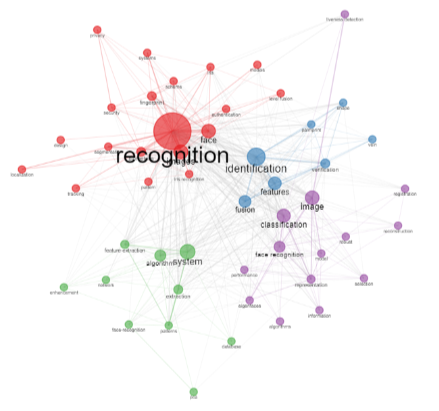
\includegraphics[width=1\textwidth]{experiments/DYosplay/PesquisaBibliometrica/Imagens/BIPA@DYosplay_CoOcurrenceNetwork1993-2022.png}
    \caption{Co-ocorrência de palavras-chaves no conjunto de dados BIBA@DYosplay no período de 1993 até 2022.}
    \label{fig:CoOcurrence1993-2022:BIPA@DYosplay}
\end{figure}


\subsection{Análise Descritiva da base de dados BIPA@DYosplay}

Abaixo se encontram as informações mais gerais da base de dados BIPA@DYosplay.

\begin{description}
    \item [``Timespan''] Após a pesquisa e filtragem os artigos resultantes foram publicados entre 1993 e 2022.
    
    \item [``Sources (Journals, Books, etc)]" No total 513 fontes de informação diferentes estão presentes na base de dados, o que dá uma média de quase 4 artigos para cada fonte de informação.
    
    \item [``Average years from publication'']  A média de tempo de publicação dos artigos é de 6,07 anos.
    
    \item [``Average citations per documents''] A média de citações por documento é de 19,17.
    
    \item [``Average citations per year per doc''] A média de citações por ano de cada artigo, a contar de sua data de publicação, é de 2,057.
    
    \item [ "References''] O conjunto de dados contém 45.581 referências citadas.
    
    \item [``Keywords Plus (ID)" ] 1.422 palavras-chaves distintas aparecem no conjunto de dados.
    
    \item [``Author's Keywords (DE)''] 5.650 palavras-chaves indicadas pelos autores estão presentes no conjunto de dados.
    
    \item [``Authors''] 5.040 nomes distintos de autores foram encontrados na base de dados.
    
    \item [``Author Appearances''] os 5.040 autores aparecem em 7.248 ocorrência pelo conjunto de  dados.
    
    \item [``Authors of single-authored documents''] Dos 5.040 autores encontrados, 79 assinam a autoria do artigo individualmente.
    
    \item [``Authors of multi-authored documents''] Dos 5.040 autores encontrados, 4961 editaram artigos em conjunto.
    
    \item [``Single-authored documents''] 88 artigos foram feitos por um único autor. Os demais foram feitos por mais de um autor.
    
    \item [``Documents per Author''] Cada um dos 5.040 nomes distintos de autores encontrados publicou em média 0.4 artigos.
    
    \item [``Authors per Document''] A média de autores por documento no conjunto de dados é de 2,5
    
    \item [``Co-Authors per Documents''] A média de co-autores por documento é de 3,6.
    
    \item [``Collaboration Index''] Os 5.040 nomes de autores encontrados colaboraram em média 2,58 vezes para editar os  1.926 artigos elaborados em co-autoria.
    
\end{description}

\subsection{Evolução da Produção Científica}
\label{DYosplay_prodcient}
A figura \ref{fig:evol:anual:BIPA@DYosplay} mostra a evolução da produção cientifica com base nos artigos sobre biometria presentes no conjunto de dados BIPA@DYosplay.

\begin{figure}[H]
    \centering
    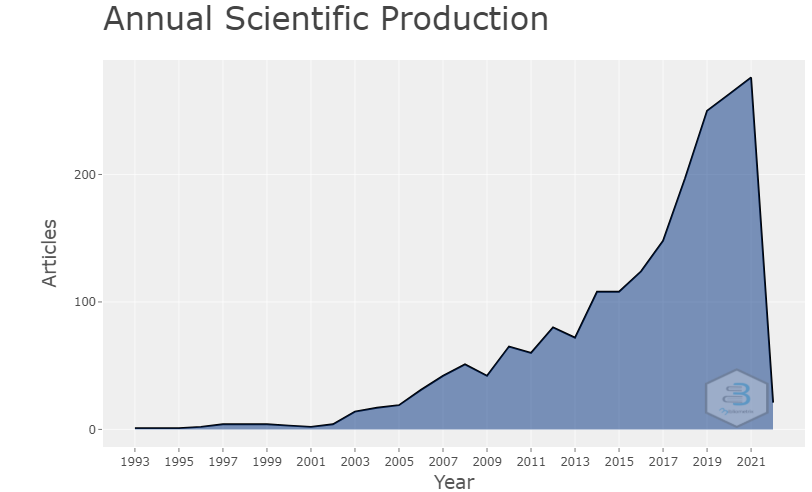
\includegraphics[width=1\textwidth]{experiments/DYosplay/PesquisaBibliometrica/Imagens/BIPA@DYosplay_Annual Scientific Production.png}
    \caption{Evolução da produção científica no conjunto de dados BIPA@DYosplay.}
    \label{fig:evol:anual:BIPA@DYosplay}
\end{figure}

A taxa de crescimento é de 11.07\% ao ano, o que justifica o formato exponencial da curva.

Os registros começam a partir do ano de 1993 e permanecem relativamente constantes até 2002, com um suave crescimento seguido de queda entre os anos de 1997 e 1999.

É só a partir de 2002, quase 10 anos após o início das publicações presentes no conjunto de dados que o crescimento se demonstra mais significativo, aumentando consideravelmente ano após ano até 2008, que marca o início de uma queda na produção científica, ao menos no que diz respeito a esse conjunto de dados.

Entre 2008 e 2014 percebemos que o comportamento se repete: um aumento seguido de queda, novamente seguido de um aumento e assim sucessivamente.

Entre 2014 e 2015 a produção se mantém estável, até que a partir de 2015 o crescimento se acentua, chegando a explodir por volta de 2017, quando acontece um crescimento sem precedentes, que se mantém até os dias de hoje.

\subsubsection{Interpretação da Curva da Evolução da Produção Científica}

A biometria é um assunto relativamente novo e tem como principal objetivo oferecer mais segurança a processos de autenticação, mas o que a curva de produção científica pode nos dizer sobre a evolução na área?

O primeiro período interessante é o que ocorre entre 1993 e 2002, período marcado pela baixa produção e que antecede o primeiro crescimento significativo. A figura \ref{fig:CoOcurrence1993-2002:BIPA@DYosplay} mostra a co-ocorrência de palavras chaves nesse período. A partir dela podemos perceber a existência de apenas duas palavras chaves principais: \textit{eigenfaces} (autofaces), que se refere ao reconhecimento de faces e \textit{templates} (modelos), relacionados com sistemas. Isso sugere que nesse período inicial o foco se concentrava principalmente em biometria facial.

\begin{figure}[H]
    \centering
    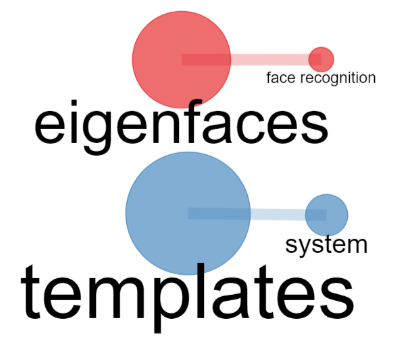
\includegraphics[width=0.5\textwidth]{experiments/DYosplay/PesquisaBibliometrica/Imagens/BIPA@DYosplay_CoOcurrenceNetwork1993-2002.png}
    \caption{Co-ocorrência de palavras chaves no período de 1993 até 2002 no conjunto de dados BIPA@DYosplay.}
    \label{fig:CoOcurrence1993-2002:BIPA@DYosplay}
\end{figure}

O segundo período interessante ocorre entre 2002 e 2015, quando observamos um maior crescimento, embora ainda com algumas baixas ocasionais.

\begin{figure}[H]
    \centering
    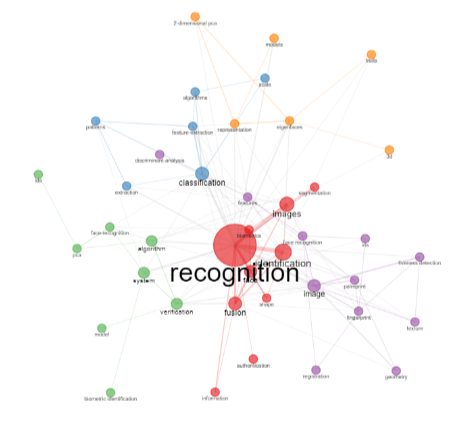
\includegraphics[width=1\textwidth]{experiments/DYosplay/PesquisaBibliometrica/Imagens/BIPA@DYosplay_CoOcurrenceNetwork2002-2015.png}
    \caption{Co-ocorrência de palavras chaves no período de 2002 até 2015 no conjunto de dados BIPA@DYosplay.}
    \label{fig:CoOcurrence2002-2015:BIPA@DYosplay}
\end{figure}

Na figura \ref{fig:CoOcurrence2002-2015:BIPA@DYosplay} observamos em destaque a palavra-chave \textit{recognition} (reconhecimento), relacionada com termos como imagens, face e autenticação, além de, é claro, biometria. Ela marca o centro do assunto, o que é totalmente compreensível. Observamos também a aparição, em vermelho, de \textit{fusion} (fusão) que, como o nome sugere, se refere a mistura de diferentes técnicas de reconhecimento biométrico para aprimorar os resultados. Outro núcleo é o presente em laranja, que possui a palavra chave \textit{eigenfaces} (autofaces), já presente nas ocorrências mostradas na figura \ref{fig:CoOcurrence1993-2002:BIPA@DYosplay}, Em verde e azul percebemos palavras-chaves como modelo, sistemas, algoritmos, extração de características e classificação, que claramente tem relação com como o processo de reconhecimento é realizado. Já em roxo percebemos os objetos sobre os quais os processos acontecerão, como reconhecimento fácil, de iris, digital e impressão palmar.

O terceiro cenário interessante de se analisar é o que compreende o período de 2017 até 2019, quando ocorre a explosão na produção.

\begin{figure}[H]
    \centering
    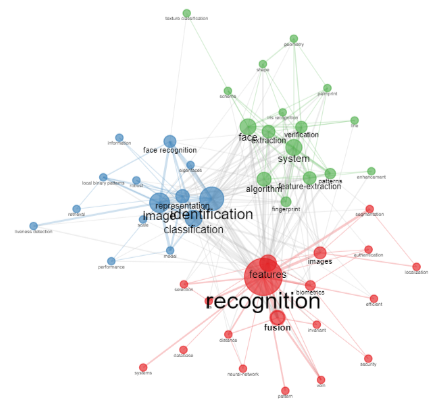
\includegraphics[width=1\textwidth]{experiments/DYosplay/PesquisaBibliometrica/Imagens/BIPA@DYosplay_CoOcurrenceNetwork2017-2019.png}
    \caption{Co-ocorrência de palavras chaves no período de 2017 até 2019 no conjunto de dados BIPA@DYosplay.}
    \label{fig:CoOcurrence2017-2019:BIPA@DYosplay}
\end{figure}

No período mostrado na figura \ref{fig:CoOcurrence2017-2019:BIPA@DYosplay} podemos observar que agora reconhecimento (\textit{recognition}) possui ligações com termos como \textit{ROI localization} (localização de regiões de interesse) e \textit{vein} (veias), o que sugere novos modelos de identificação biométrica.

\subsection{Evolução das Citações}

A figura \ref{fig:evol:anual:citacoes:BIPA@DYosplay} mostra a evolução no número de citações nos 2014 artigos presentes no conjunto de dados BIPA@DYosplay. 

Ao observar a figura percebemos que durante a maior parte do período o número de citações se mantém relativamente estável, com ocasionais picos nos anos de 1997 e 2003. Enquanto em 1997 a produção ainda era pequena, em 2003 foi quando observamos o primeiro crescimento na produção científica na área como visto na seção \ref{DYosplay_prodcient}. 

O que chama a atenção no entanto é o período inicial com alto número de citações, reflexo da baixa quantidade de artigos no momento.

\begin{figure}[H]
    \centering
    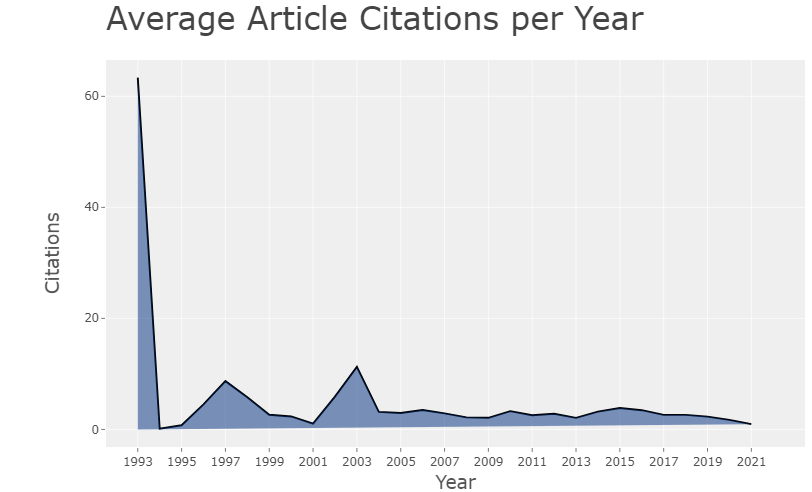
\includegraphics[width=1\textwidth]{experiments/DYosplay/PesquisaBibliometrica/Imagens/BIPA@DYosplay_Avarage Citations per Year.png}
    \caption{Evolução das citações no conjunto de dados BIPA@DYosplay.}
    \label{fig:evol:anual:citacoes:BIPA@DYosplay}
\end{figure}

\subsubsection{Interpretação da Curva de Citações por Ano}

Embora a curva de produção cientifica possua um formato exponencial, o número de citações se mantém relativamente constante ao longo de todo o período, com cada artigo no conjunto de dados sendo citado em média cerca de 3 vezes por ano.

\subsection{De onde vem essa produção científica}
\label{sec:BIPA@DYosplay_OrigemProducao}
A figura \ref{fig:MostRelevantSourcesBIPA@DYosplay} apresenta as principais fontes dos artigos presentes no conjunto de dados BIPA@DYosplay, com destaque para as revistas \textit{IEEE Transactions on Information Forensics and Security}, \textit{IEEE Acces} e \textit{Multimedia Tools and Applications}.

\begin{figure}[H]
    \centering
    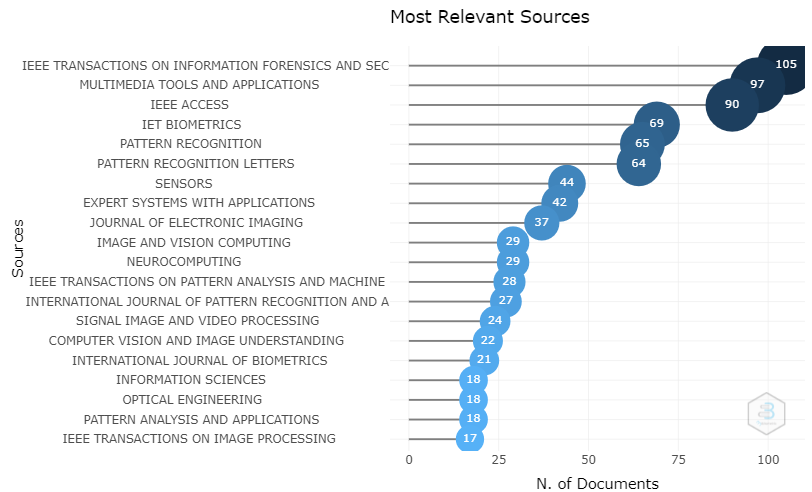
\includegraphics[width=1\textwidth]{experiments/DYosplay/PesquisaBibliometrica/Imagens/BIPA@DYosplay_MostRelevantSources.png}
    \caption{Fontes mais relevantes no conjunto de dados BIPA@DYosplay.}
    \label{fig:MostRelevantSourcesBIPA@DYosplay}
\end{figure}

A figura \ref{fig:BradfordLawBIPA@DYosplay} por sua vez mostra que o conjunto de dados BIPA@DYosplay de fato está de acordo com a lei de Bradford, que estima que os resultados de pesquisas por referências em fontes científicas tendem a diminuir exponencialmente.

Já a figura \ref{fig:MostRelevantCountriesBIPA@DYosplay} mostra os países mais citados, com destaque para a China, Estados Unidos e Inglaterra, o que faz todo sentido ao analisarmos os nomes dos autores mais relevantes na figura \ref{fig:MostRelevantAuBIPA@DYosplay} e tentarmos prever suas nacionalidades.

\begin{figure}[H]
    \centering
    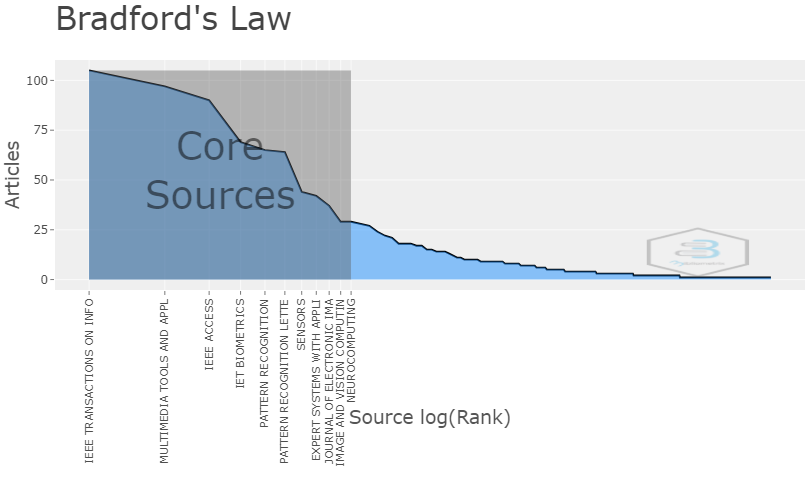
\includegraphics[width=1\textwidth]{experiments/DYosplay/PesquisaBibliometrica/Imagens/BIPA@DYosplay_BradfordLaw.png}
    \caption{Lei de Bradford no conjunto de dados BIPA@DYosplay.}
    \label{fig:BradfordLawBIPA@DYosplay}
\end{figure}

\begin{figure}[H]
    \centering
    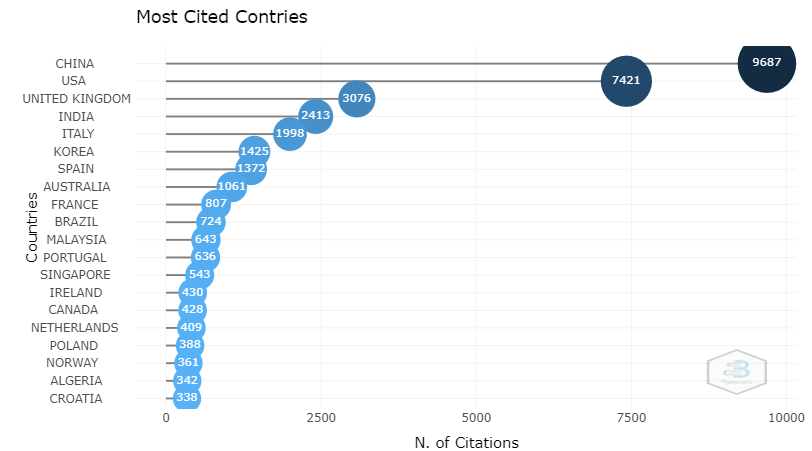
\includegraphics[width=1\textwidth]{experiments/DYosplay/PesquisaBibliometrica/Imagens/BIPA@DYosplay_MostRelevantCountries.png}
    \caption{Países mais citados no conjunto de dados BIPA@DYosplay.}
    \label{fig:MostRelevantCountriesBIPA@DYosplay}
\end{figure}

\begin{figure}[H]
    \centering
    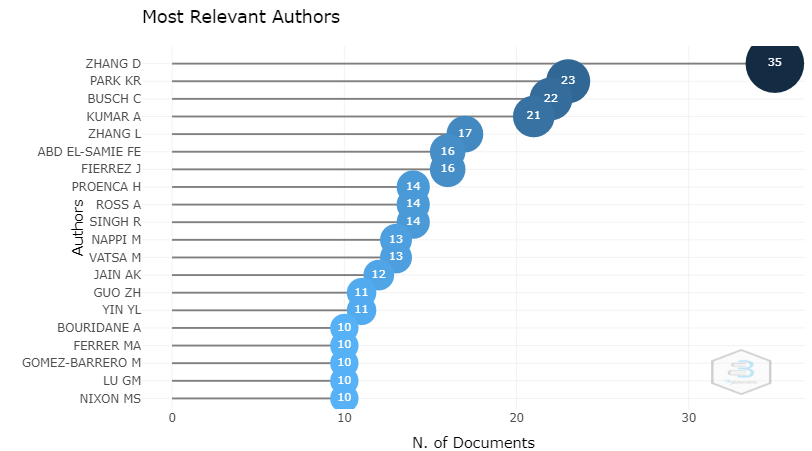
\includegraphics[width=1\textwidth]{experiments/DYosplay/PesquisaBibliometrica/Imagens/BIPA@DYosplay_MostRelevantAu.png}
    \caption{Autores mais relevantes no conjunto de dados BIPA@DYosplay.}
    \label{fig:MostRelevantAuBIPA@DYosplay}
\end{figure}

\subsection{Os artigos mais relevantes}
\label{sec:BIPA@DYosplayArtigosMaisRelevantes}

O gráfico da figura \ref{fig:GLOBALBIPA@DYOSPLAY} mostra os artigos mais citados, bem como o número de citações, do conjunto de dados BIPA@DYosplay globalmente na base de dados da \textit{Web of Science}. Isso significa que o gráfico em questão leva em conta todos os artigos presentes na \textit{Web of Science}, não se limitando aos presentes no conjunto de dados BIPA@DYosplay.

No gráfico percebemos que o artigo com maior destaque é de autoria de J. G. Daugman, seu título é: \textit{High confidence visual recognition of persons by a test of statistical independence}, que descreve um método rápido de reconhecimento biométrico a partir da íris da pessoa utilizando decisões estatísticas a partir de comparações com OU-exclusivos.

\begin{figure}[H]
    \centering
    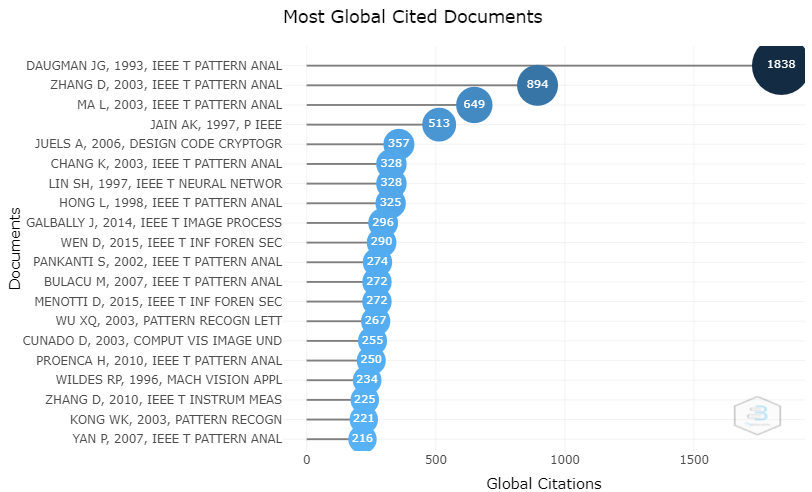
\includegraphics[width=1\textwidth]{experiments/DYosplay/PesquisaBibliometrica/Imagens/BIPA@DYosplay_GlobalArticles.png}
    \caption{Documentos no conjunto BIPA@DYosplay mais citados globalmente na \textit{Web of Science}}
    \label{fig:GLOBALBIPA@DYOSPLAY}
\end{figure}


Já a figura \ref{fig:LOCALBIPA@DYOSPLAY} apresenta os artigos mais citados, bem como o número de citações, internamente no conjunto de dados BIPA@DYosplay.

Note que o artigo mais citado é o mesmo que aparece no topo da figura \ref{fig:GLOBALBIPA@DYOSPLAY}, com praticamente o triplo das citações do segundo colocado. É interessante notar que o ano de publicação desse artigo é 1993, o que evidencia a sua importância dentro da área, assim como a relevância do autor.

\begin{figure}[H]
    \centering
    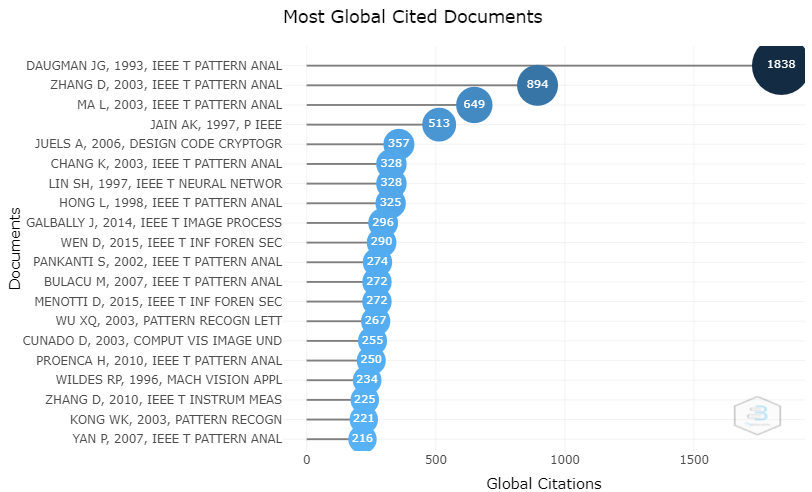
\includegraphics[width=1\textwidth]{experiments/DYosplay/PesquisaBibliometrica/Imagens/BIPA@DYosplay_GlobalArticles.png}
    \caption{Documentos no conjunto BIPA@DYosplay mais citados localmente}
    \label{fig:LOCALBIPA@DYOSPLAY}
\end{figure}


\subsection{Plotagem de Três-Campos (Diagrama de Sankey)}
\label{sec:BIPA@DYosplayPlotagemTresCampos}

A figura \ref{fig:TFP10BIPA@DYOSPLAY} apresenta a afinidade entre três conjuntos de atributos. No conjunto da esquerda se encontram as 20 citações mais frequentes (CR - \textit{Cited Record}s). No centro, encontram-se os 10 autores com maior destaque no conjunto (AU - \textit{Authors}). À direita se encontram as 20 palavras-chaves que mais aparecem (DE - \textit{Author Keywords}).

\begin{figure}[H]
    \centering
    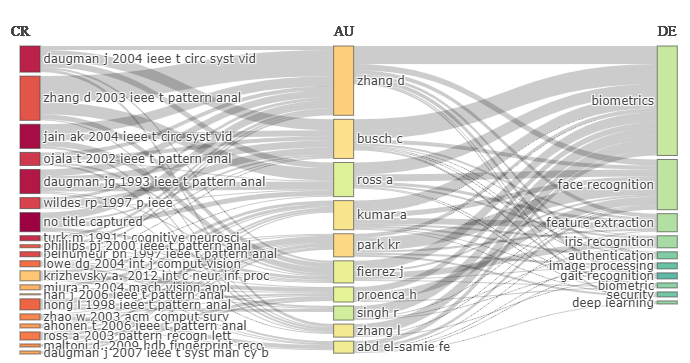
\includegraphics[width=1\textwidth]{experiments/DYosplay/PesquisaBibliometrica/Imagens/BIPA@DYosplay_Three-FieldsPlot10.png}
    \caption{Plotagem de três-campos no conjunto de dados BIPA@DYosplay}
    \label{fig:TFP10BIPA@DYOSPLAY}
\end{figure}

\subsubsection{Interpretação da Plotagem de Três-Campos}

Ao analisarmos a figura logo percebemos que "\textit{biometrics}" é a palavra-chave mais recorrente, porém se olharmos com mais atenção as demais palavras notaremos que a palavra-chave "\textit{biometric}" também aparece, o que sugere que o termo é, na realidade, ainda mais relevante. Como era de se esperar, todos os autores possuem uma conexão com o termo, diferente do último, "\textit{deep learning}", que além de aparecer pouco não está relacionado a todos os autores. Isso aconteceu devido a pesquisa ter sido objetiva, evitando, por exemplo, artigos que aparentassem ter um foco muito mais centrado em algoritmos de inteligência artificial que biometria.

Outro termo que aparece pouco é "\textit{security}", que se refere a segurança computacional e apresenta, em especial, uma ligação com autenticação. Os outros termos que aparecem eram completamente esperados dado o diagrama de co-ocorrência visto na figura \ref{fig:CoOcurrence1993-2022:BIPA@DYosplay}

Entre os autores percebemos que o mais relevante apresenta ligações com praticamente todos os termos e citam praticamente todos os registros no diagrama. Além disso, vale destacar que dois deles aparentam ter origem chinesa de acordo com o nome, enquanto não fica muito clara a nacionalidade dos demais apenas pelo nome. Outro fator interessante é que o registro mais citado é justamente o do autor com maior destaque, sendo que o mais recente é de 2012, sugerindo que nos últimos 10 anos não surgiu nada com muito destaque na área, ao menos pelo que consta neste conjunto de dados.

\subsection{Estrutura Intelectual}

\begin{figure}[H]
    \centering
    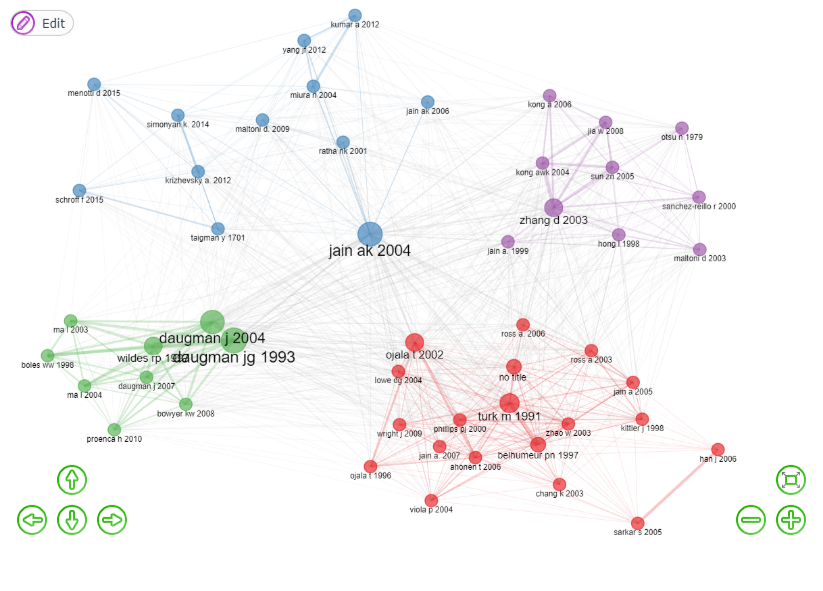
\includegraphics[width=1\textwidth]{experiments/DYosplay/PesquisaBibliometrica/Imagens/BIPA@DYosplay_CoCitation.png}
    \caption{Rede de co-citação de autores no conjunto de dados BIPA@DYosplay}
    \label{fig:CO_CITATION_BIPA@DYOSPLAY}
\end{figure}

A figura \ref{fig:CO_CITATION_BIPA@DYOSPLAY} mostra a rede co-citação de autores presentes no conjunto de dados BIPA@DYosplay. Nela, observamos quatro aglomerados principais. O aglomerado em verde tem como maior destaque o autor Daugman, o mesmo apresentado na seção \ref{sec:BIPA@DYosplayArtigosMaisRelevantes} responsável pelo artigo com maior número de citações abordado naquele momento.

O aglomerado em verde tem como maior destaque Zhang, que lidera na plotagem de três-campos apresentada na seção \ref{sec:BIPA@DYosplayPlotagemTresCampos}.

O aglomerado em azul tem como foco Jain, o que mostra que embora seja responsável por poucos artigos (apenas 12) conforme mostrado na seção \ref{sec:BIPA@DYosplay_OrigemProducao}, seu trabalho apresenta bastante relevância em campos específicos do reconhecimento biométrico.

O último aglomerado é o vermelho, onde percebemos dois autores com aparente igual relevância: Ojala e Turk. O curioso é que ambos não figuram na lista dos autores com mais publicações apresentada na seção \ref{sec:BIPA@DYosplay_OrigemProducao}, o que sugere que eles são responsáveis por artigos de grande importância na área de reconhecimento biométrico.




\chapter{Análise Bibliográfica sobre Criptografia no Universo da Computação Quântica, por André Larrosa Chimpliganond}

\section{Planejamento do estudo}
Como se transmitir informações de modo que esta só possa ser acessada pela pessoa certa? Responder essa pergunta e elaborar métodos para por a solução em prática é área de estudo da criptografia. Utilizando de alta complexidade matemática, técnicas de criptografia codificam informações de modo que só possam ser decodificadas por quem possuir a chave. Mas como o advento e evolução da computação quântica afeta a maneira como criptografamos os dados?

Partindo dessa pergunta, podemos explorar outras que irão nortear o trabalho:
\begin{itemize}
    \item Quais conceitos relacionados à esse embate entre a criptografia e computação quântica?
    \item Quais autores, instituições e nações estão à frente desse tema?
    \item Como esse conteúdo tem se desenvolvido ao longo do tempo?
\end{itemize}


\subsection{Ferramentas}
Será utilizada a interface web para o pacote Bibliometrix (Biblioshiny). O pacote Bibliometrix é uma ferramenta R que fornece um conjunto de ferramentas para a investigação quantitativa em cientometria e bibliometria.


\section{Coleta de dados}

A coleta de dados feita usando o Web Of Science  no dia 09 de fevereiro de 2022, acessado por meio do Portal de Periódicos da CAPES.

Foram feitas buscas nas coleções \textbf{Science Citation Index Expanded (SCI-EXPANDED)--1945-presente}, \textbf{Conference Proceedings Citation Index – Science (CPCI-S)--1990-presente} e \textbf{Emerging Sources Citation Index (ESCI)--2017-presente}. 

Foi usada a seguinte \query\  de busca

\textit{\textbf{(quantum or  post-quantum) and (cryptography or cryptanalysis or encryption)}}


%\lstinputlisting[numbers=left,basicstyle=\normalsize\ttfamily,caption={\query\  de busca sobre criptografia quântica.}, label=CQA@andrelarrosacryptQuery]%label
%{experiments/andrelarrosacrypt/AnaliseBibliometrica/CriptografiaQuantica/query.txt}
%nao ta achando a query


\subsection{Explicação para os termos de busca usados}

Foram elaboradas duas cláusulas de busca unidas por \textit{and}. A primeira foca nos elementos relacionados ao universo quântico, enquanto a segunda faz referência à criptografia.

Os 10522 registros obtidos encontram-se no github do projeto, em \url{https://github.com/jhcf/Comput-Experim-20212/experiments/andrelarrosacrypt/AnaliseBibliometrica/CriptografiaQuantica/rec_1.txt} e \url{https://github.com/jhcf/Comput-Experim-20212/experiments/andrelarrosacrypt/AnaliseBibliometrica/CriptografiaQuantica/rec_2.txt}. 
% arquivo maior que  50MB

Foram exportadas todas as informações disponíveis na Web Of Science de cada documento.

\section{Análise dos dados}

\subsection{Filtragem de registros}


Após carregar o dataset na plataforma biblioshiny, foi feita uma filtragem dos documentos com o intuito de selecionar apenas os artigos publicados em revistas científicas (\textit{ARTICLE}). Após a filtragem, sobraram 7131 documentos. Esse novo dataset será nomeado CriptografiaQuanticaArtigos ou CQA@andrelarrosacrypt.

\subsection{Informações principais do \dataset\   CQA@andrelarrosacrypt}
\begin{description}
    \item[Período]	1988 - 2022
    \item[Fontes]	675
    \item[Documentos]	7131
    \item[Média de tempo de publicação]	8.31
    \item[Média de citações por documento]	33.05
    \item[Média de citações por ano por documento]	2.75
    \item[Referências]	83981
    \item[Palavras-chave (Keywords Plus (ID))]   3187
    \item[Palavras-chave (Author's Keywords (DE))] 8201
    \item[Autores]   10925
    \item[Aparições de autores]	28034
    \item[Autores de documentos de autoria única]	436
    \item[Autores de documentos de autoria múltipla]	10489
    \item[Documentos de autoria única]	706
    \item[Média de documentos por autor]	0.653
    \item[Média de autores por documento]	1.53
    \item[Média de co-autores por documento]	3.93
    \item[Index de colaboração]        1.63
\end{description}


\subsection{Evolução da Produção Científica}

\begin{figure}
    \centering
    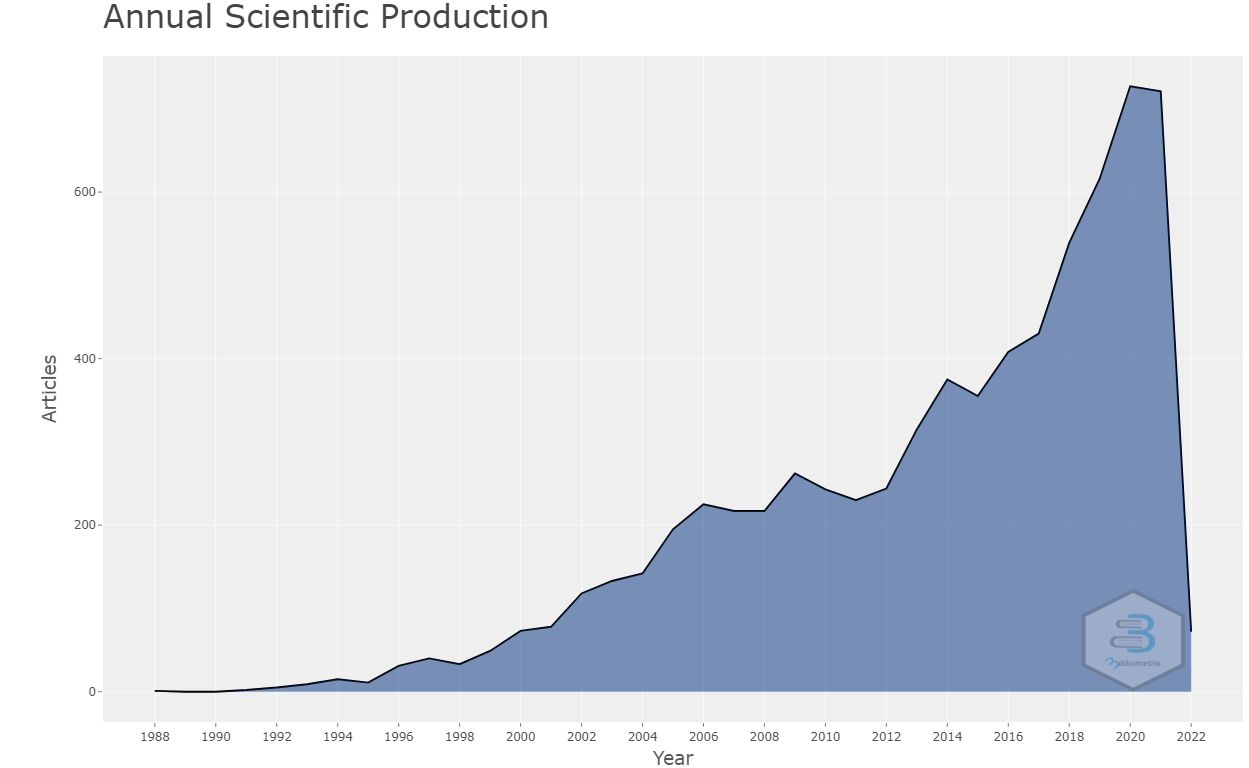
\includegraphics[width=1\textwidth]{experiments/andrelarrosacrypt/AnaliseBibliometrica/CriptografiaQuantica/imagens/CQA@andrelarrosacrypt_ProdAnual.png}
    \caption{Evolução da produção científica no \dataset\ CQA@andrelarrosacrypt.}
    \label{CQA@andrelarrosacrypt_ProdAnual}
\end{figure}

A figura \ref{CQA@andrelarrosacrypt_ProdAnual} representa a evolução da produção de documentos relacionados ao tema do \dataset\ CQA@andrelarrosacrypt, de 1988 até 2022. Como os dados foram coletados no início de 2022, a produção específica desse ano ainda é baixa, mas, como o gráfico segue uma curva aproximadamente exponencial, é de se esperar que acompanhe o nível de 2020 e 2021.



\subsection{Interpretação do Crescimento}

Como destacado na \href{https://www.quthought.com/post/history-of-quantum-computing-a-timeline}{Linha do Tempo}, o do desenvolvimento da computação quântica nos anos 1990 é representado na figura como o início do crescimento das pequisas. Na mesma referência, percebemos que nos últimos dez anos empreses como Google e IB, além de instituições como NASA e NSA tem investido nesse assunto. Indicando, não só um interesse econômico, mas uma necessidade governamental.

Se considerarmos os interesses da NSA (Agência de Segurança Nacional dos Estados Unidos), percebemos como esse novo tipo de computação está alterando a meneia como vemos codificação e decodificação de informações. 


\subsection{Evolução das Citações}

\begin{figure}
    \centering
    \includegraphics[width=1\textwidth]{experiments/andrelarrosacrypt/AnaliseBibliometrica/CriptografiaQuantica/imagens/CQA@andrelarrosacrypt_CitaAnual.png}
    \caption{Evolução das citações ao \dataset\ CQA@andrelarrosacrypt.}
    \label{CQA@andrelarrosacrypt_CitaAnual}
\end{figure}

% media das citacoes ?????/

Como mostrado na figura \ref{CQA@andrelarrosacrypt_CitaAnual}, com exceção aos anos 1990 e 1991, os documentos apresentam uma média de ???.


\subsection{Interpretação das Citações}

% n de citacoes nao cresce



% artigos mais importantes ???


\subsection{\textit{Three-Field Plots}}

Gráficos do tipo \textit{Three-Field Plots} exibem três campos (autores, documentos, referências, entre outros) e como eles se relacionam (\textit{Sankey Diagram}).

\subsubsection{\textit{Three-Field Plots} Autores, Referências e Palavras-chave}

\begin{figure}
    \centering
    \includegraphics[angle=0,width=1\textwidth]{experiments/andrelarrosacrypt/AnaliseBibliometrica/CriptografiaQuantica/imagens/CQA@andrelarrosacrypt_Aut_Ref_Key.png}
    \caption{\textit{Three-Field Plots} do \dataset\ CQA@andrelarrosacrypt: 20 Autores, 20 Referências e 20 Palavras-Chave mais relevantes.}
    \label{CQA@andrelarrosacrypt_Aut_Ref_Key}
\end{figure}

A figura \ref{CQA@andrelarrosacrypt_Aut_Ref_Key} apresenta o gráfico \textit{Three-Field Plots} do  \dataset\ CQA@andrelarrosacrypt. Os campos de interesse destacados nesse gráfico são autores (centro), referência citadas (esquerda) e palavras-chave (direita) mais importantes.

No campo \textit{autores}, percebemos que 19 aparentam ser de origem asiática (mais provavelmente chinesa), o único não asiático provavelmente é russo (molotkov sn). Por outro lado, as referências apresentam maior heterogeneidade, com documentos aparentemente asiáticos, europeus e norte-americanos. Isso nos sugere que pesquisadores de origem chinesa tem migrado para países ocidentais ou tem trabalhado em direta colaboração com pesquisadores europeus e norte-americanos.

Relevante cometar que o autor mais destacado é \textbf{deng fg} e nas referências mais citadas temos três trabalhos de sua autoria \textbf{}{Deng FG, 2003, PHYS REV A} - DOI 10.1103/PhysRevA.68.042317 (protocolo para comunicação quântica segura), \textbf{Deng FG, 2004, PHYS REV A} - DOI 10.1103/PhysRevA.69.052319 (outro protocolo para comunicação quântica segura) e \textbf{Deng FG, 2005, PHYS REV A} - DOI 10.1103/PhysRevA.72.044302 (análise de protocolo de comunicação segura proposto por Zhang, Li, and Man). O que nos mostra a relevância de tal autor e seu aparente foco na área de comunicação segura.

Ao estudarmos as \textit{palavras-chaves} fica claro o focos desses autores no temos de comunicação quântica segura, \textbf{quantum secure direct communication}, \textbf{quantum secret sharing} e \textbf{quantum communication}, e o uso de criptografia quântica, \textbf{quantum cryptography} e \textbf{quantum key distribution}, para tal fim.


\subsubsection{\textit{Three-Field Plots} Autores, Afiliações e Países}

\begin{figure}
    \centering
    \includegraphics[angle=0,width=1\textwidth]{experiments/andrelarrosacrypt/AnaliseBibliometrica/CriptografiaQuantica/imagens/CQA@andrelarrosacrypt_Aut_Aff_Coun.png}
    \caption{\textit{Three-Field Plots} do \dataset\ CQA@andrelarrosacrypt: 20 Autores, 20 Instituições e 20 Países mais relevantes.}
    \label{CQA@andrelarrosacrypt_Aut_Aff_Coun}
\end{figure}


O gráfico da figura \ref{CQA@andrelarrosacrypt_Aut_Aff_Coun} confirma as suspeitas em relação à origem chinesas da maioria dos autores. Mesmo com a prevalência da China, temos a Rússia, Canada, Suíça, Alemanha, França e Estados Unidos com significativa influência.

Com relação às instituições afiliadas, notamos um predomínio das universidades chinesas, o que pode indicar que esses pesquisadores chineses estão trabalhando na China e não em universidades estrangeirais como havia sido sugerido. Observando o campo dos países, percebemos que muitos dos pesquisadores chineses tem afiliações com outros países. Isso indica que a segunda teoria apontada anteriormente, colaboração com pesquisadores ocidentais, parece ser verdade.

\section{Estrutura Conceitual}

\begin{figure}
    \centering
    \includegraphics[angle=0,width=1\textwidth]{experiments/andrelarrosacrypt/AnaliseBibliometrica/CriptografiaQuantica/imagens/CQA@andrelarrosacrypt_MapaTematico.png}
    \caption{Mapa temático do \dataset\ CQA@andrelarrosacrypt.}
    \label{CQA@andrelarrosacrypt_MapaTematico}
\end{figure}

Fazendo um estudo da figura \ref{CQA@andrelarrosacrypt_MapaTematico} identificamos cinco aglomerados de conceitos que definem as principais áreas de estudo. Termos como \textbf{cryptograpy}, \textbf{quantum cryptograpy}, \textbf{entanglement}, \textbf{algorithm}  são esperados considerando o tema do nosso estudo. O que mais interessa são as expressões que, a priori, não parecem condizer com a pesquisa, essas que vamos focar.

Primeiro, temos em azul duas palavras que necessitam de explicação, \textbf{scheme} e \textbf{protocol}. Ambas fazem referência à comunicação segura e suas regras no mundo quântico. Passando para o aglomerado vermelho, encontramos \textbf{key distribution} está relacionado à um problema em criptografia que envolve a distribuição de chaves de acesso às partes interessadas, o que faz sentido considerando as demais expressões nesse mesmo aglomerado. Com relação ao agregado verde, temos \textbf{teleportation}. Ela se refere à teletransportação quântica, um método de se transferir informação quântica. Por fim, temos o bloco roxo, \textbf{light}, \textbf{emission} e \textbf{transmission}, todos apontam para as ótica quântica que estuda, dentre outras coisas, o uso de fótons de luz para transportar/processar informação.

\section{Estrutura Intelectual}

\begin{figure}
    \centering
    \includegraphics[angle=0,width=1\textwidth]{experiments/andrelarrosacrypt/AnaliseBibliometrica/CriptografiaQuantica/imagens/CQA@andrelarrosacrypt_CoCit.png}
    \caption{Rede de co-citação do \dataset\ CQA@andrelarrosacrypt.}
    \label{CQA@andrelarrosacrypt_CoCit}
\end{figure}

Com relação à estrutura intelectual visível na figura \ref{CQA@andrelarrosacrypt_CoCit}, temos três principais grupos. Em vermelho encontramos o que parecem ser autores ocidentais, em azul autores chineses e em verde autores ocidentais e chineses. Podemos esperar que os autores de cada grupo estegem trabalhando em temas semelhantes

O autor de maior influência no grupo vermelho é \textit{Bennett}. Seus dois artigos mais citados, ambos de 1992, \textit{Quantum cryptography using any two nonorthogonal states} e \textit{Quantum cryptography without Bell’s theorem}. Como podemos perceber, tratam de estratégia e técnicas de criptografia quântica. Podemos esperar que os autores que citam Bennett também desenvolvem desse assunto. Para confirmar nossas suspeitas, temos \textit{Ekert} e seu artigo \textit{Quantum cryptography based on Bell’s theorem}, que também aborda diretamente a questão da criptografia.

No aglomerado azul, todos parecem estar no mesmo nível, no que diz respeito à citações. Pegando como exemplo \textit{Deng}, seu artigo mais citado é \textit{Two-step quantum direct communication protocol using the Einstein-Podolsky-Rosen pair block}, que trata de protocolo de comunicação apoiado em aspectos da teoria quântica. Se selecionarmos outro autor do mesmo grupo, \textit{Li}, vemos que seu trabalho mais citado, \textit{Improving the security of secure direct communication based on the secret transmitting order of particles} também trata de comunicação. Logo, parece seguro afirmar que esse grupo foca em elemento de comunicação (segura) utilizando fatores da teoria quântica.

Por fim, no grupo verde, temos \textit{Lo} como influente autor. Seu trabalho mais citado localmente \textit{Unconditional Security of Quantum Key Distribution over Arbitrarily Long Distances} aborda comunicação segura (como o grupo azul) sob o ponto de vista de chave chave distribuída. Novamente, se observarmos o trabalho de \textit{Gisin}, \textit{Trojan-horse attacks on quantum-key-distribution systems}, vemos o mesmo tópico.


% o que mais ??

\section{Estrutura Social}

\begin{figure}
    \centering
    \includegraphics[angle=0,width=1\textwidth]{experiments/andrelarrosacrypt/AnaliseBibliometrica/CriptografiaQuantica/imagens/CQA@andrelarrosacrypt_Colab.png}
    \caption{Rede de colaboração do \dataset\ CQA@andrelarrosacrypt.}
    \label{CQA@andrelarrosacrypt_Colab}
\end{figure}

Na figura \ref{CQA@andrelarrosacrypt_Colab} vemos as colaborações entre autores. Os grupos parecem ser divididos em instituições, com exceção dos autores em rosa que são de instituições distintas. O grupo rosa parece correlacionar com as colaborações entre pesquisadores chineses e ocidentais descrita anteriormente.

\begin{figure}
    \centering
    \includegraphics[angle=0,width=1\textwidth]{experiments/andrelarrosacrypt/AnaliseBibliometrica/CriptografiaQuantica/imagens/CQA@andrelarrosacrypt_ColabMap.png}
    \caption{Mapa de colaboração do \dataset\ CQA@andrelarrosacrypt.}
    \label{CQA@andrelarrosacrypt_ColabMap}
\end{figure}

Complementando as informações anteriores, na figura \ref{CQA@andrelarrosacrypt_ColabMap} evidencia as colaborações entre:

\begin{itemize}
    \item China - Estados Unidos
    \item China - Canada
    \item China - Alemanha
    \item China - Reino Unido
    \item Estados Unidos - Canada
    \item Estados Unidos - Reino Unido
\end{itemize}

Com enfase na relação Estados Unidos - China. Esses dados estão de acordo com o cenário geral de pesquisa científica, com norte-americanos e chineses dominando as áreas de conhecimento.

%\chapter{Análise Bibliográfica sobre Mineração de Dados Educacionais, por Pedro de Torres Maschio\label{chap:bibliometria:pedro-maschio}}


\section{Planejamento do estudo}

O crescente uso de plataformas de aprendizagem remota, conhecidos como Ambientes Virtuais de Aprendizagem (AVAs) aumentou consideravelmente a produção de dados sobre como os alunos aprendem e sobre como usam estas plataformas. Essa crescente quantidade de informação deu origem a um tipo de mineração de dados específica, a Mineração de Dados Educacionais. O presente estudo busca evidenciar aspectos a respeito da produção científica sobre esse tema. As questões de pesquisa são:

\begin{itemize}
    \item Como a produção científica em Mineração de Dados Educacionais evoluiu ao longo do tempo?
    \item Quais são os principais conceitos relacionados a Mineração de Dados Educacionais?
    \item Como a Mineração de Dados Educacionais tem sido utilizada para subsidiar ações práticas de ensino remoto?
\end{itemize}

\section{Coleta de dados}

A coleta de dados se deu pelo Web of Science (WeS) no dia 6 de Fevereiro de 2022. O acesso foi feito por meio do Periódicos Capes. A base que foi utilizada para a busca foi "Science Citation Index Expanded", que reúne artigos da área de ciências exatas. A \textit{string} de busca pode ser vista na listagem de código \ref{pedro-maschio:listagem}

\lstinputlisting[numbers=left,basicstyle=\normalsize\ttfamily,caption={\query\ de busca sobre Mineração de Dados Educacionais.},label=pedro-maschio:listagem]
{experiments/pedro-maschio/PesquisaBibliogr/queries/query.txt}


Inicialmente, havia sido utilizado apenas o termo "educacional data mining", após uma análise dos resultados, observou-se que uma considerável parte dos resultados tratavam-se de revisões de literatura sobre o tema, sendo assim, adicionou-se a cláusula "not review" à \textit{string} de busca.
O uso desse termo de busca resultou em 5.156 resultados na WeS. A exportação desses registros foi feita com o uso da opção "Exportar arquivo de texto sem formatação", o conteúdo foi definido com a seleção personalizada de todos os 29 campos disponíveis para marcação. Os registros foram extraídos de mil em mil e depois concatenados no único arquivo de texto de forma manual.

\subsection{Filtragem dos dados}

Após a coleta, foram considerados somente registros de artigos científicos publicados em períodicos. Sendo assim, restaram 4.700 registros para análise. De agora em diante esse conjunto de registros será chamado EDM@pedro-maschio.

\section{Análise dos dados}

\subsection{Análise descritiva}

O bibliometrix, por meio da interface biblioshiny permite extrair uma tabela contendo as principais informações sobre os artigos contidos no EDM@pedro-maschio, abaixo estão listadas algumas dessas informações:
\begin{description}
    \item[Timespan] os artigos do \textit{dataset} EDM@pedro-maschio abrangem os anos de 1991 a 2022, o que ressalta o quão novo é o campo de estudo em Mineração de Dados Educacionais, tendo em vista que não foram encontrados artigos entre 1945 e 1990.
    \item[Sources (Journals, Books, etc)] há 1445 fontes de informação no \textit{dataset} EDM@pedro-maschio.
    \item[Documents] há 4700 documentos no \textit{dataset} EDM@pedro-maschio, sendo todos artigos científicos.
    \item[Average years from publication] a média de anos de publicação do \textit{dataset} EDM@pedro-maschio é de 4.46.
    \item[Average citations per documents] a média de citações por documento é de 14.4 no \textit{dataset} EDM@pedro-maschio.
    \item[Average citations per year per doc] a média de citações por ano por documento é de 2.349 no \textit{dataset} EDM@pedro-maschio.
    \item[References] há 169101 referências no \textit{dataset} EDM@pedro-maschio.
    \item[Keywords Plus (ID)] há 9501 Keywords Plus (ID) no \textit{dataset} EDM@pedro-maschio.
    \item[Author's Keywords (DE)] há 14652 palavras-chave que foram adicionadas pelos autores no \textit{dataset} EDM@pedro-maschio.
    \item[Authors] há 14911 nomes de autores distintos no \textit{dataset} EDM@pedro-maschio
    \item[Author Appearances] os 14911 autores distintos aparecem 28196 no \textit{dataset} EDM@pedro-maschio.
    \item[Authors of single-authored documents] 111 autoes publicaram artigos sem co-autores no \textit{dataset} EDM@pedro-maschio.
    \item[Authors of multi-authored documents] 14800 autores foram autores de artigos em conjunto com outros autores no \textit{dataset} EDM@pedro-maschio.
    \item[Single-authored documents] 128 artigos foram escritos por um único autor no \textit{dataset} EDM@pedro-maschio.
    \item[Documents per Author] a taxa de documentos por autor é de 0.315 no \textit{dataset} EDM@pedro-maschio.
    \item[Authors per Document] a taxa de autor por documento é de 3.17 no \textit{dataset} EDM@pedro-maschio.
    \item[Co-Authors per Documents] há em média 6 autores por artigos no \textit{dataset} EDM@pedro-maschio.
    \item[Collaboration Index] o índice de colaboração é de 3,24 no \textit{dataset} EDM@pedro-maschio.
\end{description}

\section{Visualização dos dados}

\subsection{Evolução da produção Científica}

\begin{figure}[H]
    \centering
    \includegraphics[width=1\textwidth]{experiments/pedro-maschio/PesquisaBibliogr/MineracaoDadosEducacionais/images/crescimento-anual.png}
    \caption{Evolução da produção científica no \textit{dataset} EDM@pedro-maschio.}
    \label{fig:evol:anual:EDM@pedro-maschio}
\end{figure}

Conforme apresenta-se na Figura \ref{fig:evol:anual:EDM@pedro-maschio}, a produção de artigos referente à Mineração de Dados Educacionais cresceu vertiginosamente, tendo seu início de fato a partir do ano 2005. A taxa média de crescimento anual foi de 17.41\%. 

\subsection{Citações média por ano}

\begin{figure}[H]
    \centering
    \includegraphics[width=1\textwidth]{experiments/pedro-maschio/PesquisaBibliogr/MineracaoDadosEducacionais/images/citacoes-media-anual.png}
    \caption{Evolução da produção científica no \textit{dataset} EDM@pedro-maschio.}
    \label{fig:citacoes:anual:EDM@pedro-maschio}
\end{figure}

Além da evolução no número de artigos publicados por ano, é possível extrair a evolução do número de citações média por ano, conforme apresenta-se na Figura \ref{fig:citacoes:anual:EDM@pedro-maschio}. Interessante notar os picos nos anos 1996, 1999 e 2006.


\subsection{Conceitos relacionados}

A análise da estrutura conceitual do documento começou pela geração do gráfico da Rede de Co-Ocorrências de Palavras-Chave. Este gráfico está evidenciado na Figura \ref{fig:co-ocorrencias:EDM@pedro-maschio}. Pela análise do gráfico gerado é possível observar a prevalência dos termos \textbf{modelo, predição, classificação, algoritmo e performance}; tais termos estão condizentes com o tema de Mineração de Dados Educacionais e dão \textit{insights} dos conceitos relacionados a essa área.

\begin{figure}[H]
    \centering
    \includegraphics[width=1\textwidth]{experiments/pedro-maschio/PesquisaBibliogr/MineracaoDadosEducacionais/images/co-ocorrencias.png}
    \caption{Rede de co-ocorrências de palavras chave do \textit{dataset} EDM@pedro-maschio.}
    \label{fig:co-ocorrencias:EDM@pedro-maschio}
\end{figure}


\section{Resultados e interpretação}

Esta pesquisa bibliográfica indicou um crescente apelo da comunidade científica por buscas no campo de Mineração de Dados Educacionais. Os picos apresentados no gráfico de citações precisam ser melhor compreendidos por meio de uma busca mais aprofundada.


%\chapter{Análise Bibliográfica sobre Programação Competitiva, por Enzo Yoshio}

\section{Planejamento do estudo}

    O planejamento de estudos é importante para os estudos científicos e o método científico pois sem um planejamento e questionamento do que a pesquisa deve procurar, o objetivo e o foco da pesquisa pode se perder sem esse planejamento e a organização dos pesquisadores feita previamente. Dito isso, durante o planejamento, é necessário levantar alguns questionamentos para nortear a pesquisa e ficar claro pros pesquisadores o alvo de pesquisa e o que eles devem solucionar. Em sequência há alguns questionamentos feitos para essa análise bibliográfica.
 

\begin{itemize}
    \item Qual a relevância da programação competitiva para a comunidade científica? 
    \item A programação competitiva tem influenciado a comunidade científica e o mercado de trabalho?
    \item A programação competitiva vem sendo popularizada nos últimos anos?
\end{itemize}

\subsection{Limitações} O artigo foi proposto em uma matéria semestral na Universidade de Brasília, sendo feito como atividade semanal para aprender os usos do R Studio e bibliometrix. Logo houve pouco tempo para o desenvolvimento do artigo buscando as fontes necessárias para que ficasse um artigo substancial e bem feito. O artigo foi feito ao longo de uma semana, usando um horário de 10 horas aproximadamente.

\section{Coleta de dados}

A coleta de dados foi realizada usando o software de busca Web Of Science no dia 8 de fevereiro de 2022, acessado por meio do Portal de Periódicos da Capes.

\subsection{Query de Busca}

Para a busca, foi usada uma \query\ abaixo:
\begin{verbatim}
(codeforces)
(compet* and program*)
(codechef)
\end{verbatim}

\subsubsection{Explicação para os termos de busca usados}

Como o foco era programação competitiva, o termo compet* e program* foram usados concatenados para buscar todas as referencias possíveis a programação competitiva, também foram usados os nomes de alguns sites famosos que a comunidade de programação científica usa bastante, sendo o mais famoso o codeforces. Não há um consenso em qual nome oficial deveria ser usado para programação competitiva, por exemplo, no Brasil também é conhecida como Maratona de Programação, algumas pessoas influentes nessa comunidade já usaram outros termos como sport of mind, programming sports, entre outros, mas definitivamente o mais famoso é competitive programming e esse é o motivo ao qual foi usado na query apenas o mais famoso, visto que os outros termos são muito pouco utilizados e não são famosos, logo a busca por esses termos não traria bons resultados na query, podendo até mesmo atrapalhar e trazer resultados indesejados, por isso a escolha de fazer a query apenas com o nome mais conhecido desse hobby e também de seus principais sites, visando a citação deles correlacionado com a programação competitiva.

\subsection{Registros recuperados}

Os 5000 registros obtidos na busca podem ser encontrados no link \url{}
Foi utilizada o opção de exportação para aquivo de texto sem formatação, contemplando todos as 29 opções de campo. Os 5000 registros foram recuperado em grupos de 1000 para posteriormente serem concatenados em um único arquivo para que o bibliometrix pudesse processá-lo.

Foram utilizadas as opções \textit{Exportar registros para arquivo de texto sem formatação} e \textit{export full record / Gravar Conteúdo: Seleção personalizada, com todos os 29 campos disponíveis, inclusive referências citadas} no Word Of Science, para que as citações também fossem usadas em análises da citações (estrutura intelectual do conhecimento). Os 5000 registros foram recuperados em 5 blocos de até 1.000 registros por vez (1-1000, 1001-2000, 2001-3000, 3001-4000, 4001-5000).

\section{Análise dos dados}

\subsection{Filtragem de registros}
Para uma melhor análise, é possível fazer o uso de filtros sobre os dados bibliométricos.

Aplicou-se uma filtragem ao \dataset prévio, com 5000 registros, em que havia prévias de artigos, artigos de conferência, capítulos de livro, entre outros... Manteve-se apenas no \dataset os artigos que foram publicados em revistas de cunho científico.\footnote{Supõe-se que os conhecimentos de maior qualidade sobre o tema em questão está nas publicações feitas em revistas.}.  Logo após aplicar essa filtragem pelo bibliometrix, 3164 registros continuaram no \dataset, que seguirá fazendo alguns processos e filtragens no bibliometrix.

Todos os documentos recolhidos tiveram uma filtragem para restar apenas os artigos que podem se encaixar como artigos os quais foram publicados em revistas científicas. Após essa filtragem, também foram tratados sob a lei de Bradford. Dos 3164 arquivos já filtrados, foram filtrados novamente para 1361 que são os documentos que serão relevantes para a análise bibliográfica sobre programação competitiva.

\subsection{Análise descritiva do \dataset\   }

Constam as informações gerais sobre os conjuntos de dados:
As informações mais gerais sobre o \dataset\   são as seguintes:
\begin{description}
    \item [\textit{Timespan}] Os artigos obtidos da busca após a filtragem foram publicados entre o período de 1991 até 2022
    \item [\textit{Sources (Journals, Books, etc)}] Os artigos possuem ao todo 163 fontes diferentes, sendo assim, em média, 8 artigos por revista.
    \item [\textit{Average years from publication}] A média de tempo de publicação dos artigos é de 5.5 anos
    \item [\textit{Average citations per documents}] A média de citações por documentos é 10.43.
    \item [\textit{Average citations per year per doc}] Após o ano de sua publicação, das um dos dos artigos foi citado em média 1.283 vezes por ano.
    \item [\textit{References}] Ao todo, foram feitas 46173  referências por entre os artigos coletados
    \item [\textit{Keywords Plus (ID)}] 2153 palavras chaves do tipo ID (Keyword Plus)
    \item [\textit{Author's Keywords (DE)}]  4383 palavras chaves escolhidas pelos autores dos artigos

    \item [\textit{Authors}]  
    \item [\textit{Author Appearances}] 
    \item [\textit{Authors of single-authored documents}] Dos 5223 autoes, 95 escreveram artigos individualmente
    \item [\textit{Authors of multi-authored documents}] Dos 5223 autores, 5138 são autores de artigos escritos em colaboração com outros.
    \item [\textit{Single-authored documents}] Dos 1361 documentos, 95 foram escritos indidualmente, o que sobrou foram produzidos em co-autoria.
    \item [\textit{Documents per Author}] A média de documentos por autor é de 0.26
    \item [\textit{Authors per Document}] A média de autores por documento é de 3.84.
    \item [\textit{Co-Authors per Documents}] As 5749 aparições de autores se distribuem em 4.22 por documento
    \item [\textit{Collaboration Index}] O indíce de colaboração (total de autores em artigos escritos em co-autoria / total de artigos escritos em co-autoria) é de 4.06.
\end{description}

As informações podem ser encontradas também na imagem abaixo:

\begin{figure}[ht]
    \centering
    \includegraphics[width=12cm]{experiments/enzoyoshio/AnaliseBibliometrica/mainInformation.PNG}
    \caption{ Principais informações sobre os dados coletados }
    \label{fig:mainInfo}
\end{figure}


\subsection{Evolução da Produção Científica}

\begin{figure}[ht]
    \centering
    \includegraphics[width=12cm]{experiments/enzoyoshio/AnaliseBibliometrica/anualScientificProduction.png}
    \caption{ Produção científica anual do \dataset\ }
    \label{fig:evoEnzoYoshio}
\end{figure}

Como pode ser observado no gráfico:

Até o ano de 2000 as publicações eram praticamente inexistentes, visto que a popularização da programação competitiva foi apenas nos anos 2000, principalmente pelo fato da criação e popularização da internet. Quanto mais pessoas começaram a ter acesso a internet, mais pessoas puderam conhecer essa nova área conhecida como computação. Logo, após os anos 2000 pudemos observar uma curva que cresce a cada ano, tendo no ano de 2021 tido seu pico de publicações e provavelmente essa curva só tende a crescer, pois mais e mais pessoas estão ingressando no mundo da programação competitiva, seja ela por ajudar em entrevistas de emprego, ou apenas pelo simples fato de conseguir aprender coisas novas e treinar o raciocínio lógico. 

\subsection{Evolução das Citações}

\begin{figure}[ht]
    \centering
    \includegraphics[width=12cm]{experiments/enzoyoshio/AnaliseBibliometrica/averageCitationPerYear.png}
    \caption{ Média de citação anual do \dataset\ }
    \label{fig:citaEnzoYoshio}
\end{figure}

A figura em \ref{fig:citaEnzoYoshio} revela quantas citações foram feitas, em média, ao longo do ano. A curva é levemente crescente e percebe-se um leve aumento a cada ano, percebe-se que há um pico em 2006, pois provavelmente foi publicado um artigo bem conceituado na área e importante para o desenvolver da área nos anos seguintes. Percebe-se uma leve queda no ano de 2021, mas isso é de se esperar, pois ainda não foram feitas referências sobre esse ano ainda. Com isso, é interessante observar essa curva de citações por ano, para entender melhor como se desenvolve essa área.

\subsection{\textit{Gráfico de três campos}}

O gráfico em \ref{fig:} mostra um gráfico de três campos feitos com os dados acerca das referências, autores e palavras-chaves mais relevantes.

\begin{figure}[ht]
    \centering
    \includegraphics[width=12cm]{experiments/enzoyoshio/AnaliseBibliometrica/threeFieldsPlot.png}
    \caption{Gráfico de três campos analisando palavras-chave no \textit{db\_GPU}}
    \label{fig:threeFieldEnzoY}
\end{figure}

Observando as palavras mais relevantes, podemos ver que tem muitos artigos em que as palavras-chave também incluem a educação, logo é importante notar a correlação entre programação competitiva e o aprendizado de alunos na graduação.

Vale ressaltar também que, há algumas palavras chaves diferentes, tendo em vista que o tema pode abordar diferentes assuntos, é complicado de fazer um filtro justamente pelo conteúdo poder abordar muitas coisas, porém podemos ver uma agregação entre os autores mais citados e as palavras-chave e suas referências.

% \chapter{Análise Bibliográfica sobre \textit{Feedbacks} Automáticos no Ensino de Programação em Cursos de Graduação, por Fernanda Macedo de Sousa \label{chap:bibliometria:fernandams}}

\section{Planejamento do estudo}

% O planejamento o  desenho do estudo deve descrever as motivações, questões de interesse, escopo, limitações e objetivos do trabalho.

O ensino de programação nos anos iniciais das graduações tem sido um grande desafio didático e metodológico. Os ambientes Virtuais de aprendizagem (AVA’s) e demais plataformas de ensino emergem como possíveis soluções para sanar as dificuldades encontradas neste processo, porém a maioria destes ambientes não dispõe da dinamicidade necessária, que é intrínseca ao processo de ensino aprendizagem e, principalmente, ao ensino da primeira linguagem de programação. Neste contexto, o presente trabalho tem como intento responder à seguinte questão de pesquisa (RQ): O que nos diz a literatura sobre o uso de feedbacks automáticos no ensino de programação em cursos de graduação nas universidades de todo o mundo? A fim de responder ao RQ foram criadas 10 questões de investigação:

\begin{itemize}
    \item RQ1). Qual é a quantidade de artigos publicados por ano relacionados a este tema? 
    \item RQ2). Quais foram os países que mais produziram estes trabalhos? 
    \item RQ3). Quais fontes de informação publicaram mais artigos sobre esse tópico?
    \item RQ4). Quais são as principais plataformas de apoio ao ensino de programação utilizados atualmente?
    \item RQ5). Quais as principais linguagens de programação (Python, C, C++, Java, etc.) mais utilizadas no ensino da primeira linguagem de programação nos cursos de graduação?
    \item RQ6). Dentre os artigos analisados, qual a porcentagem dos que apresentaram resultados positivos em relação a implementação dos sistemas de feedbacks?
    \item RQ7). Estes feedbacks foram adaptados ao perfil do aluno ou são respostas padronizadas?
    \item RQ8). Os artigos analisados apresentaram alguma forma de classificação dos discentes por meio de suas respostas?
    \item RQ9). Os artigos apresentam alguma avaliação da percepção de quem faz uso dos feedbacks automáticos?
    \item RQ10). Qual o tipo de resposta apresentada nos feedbacks?
\end{itemize}

\subsection{O que já existe de pesquisa bibliométrica sobre esse tema?}

\subsection{Uso do Bibliometrix e Biblioshiny}
% Serão usadas a ferramenta e o \textit{workflow} proposto pelos autores do pacote Bibliometrix, conforme indica a figura ~\ref{fig:bibliometrix:workflow}.

\subsection{Limitações}

\section{Coleta de dados \label{FeedAuto:coleta}}

A coleta de dados foi realizada usando a base de dados Scopus no dia 09 de fevereiro de 2022, acessada por meio do Portal de Periódicos da CAPES.

Para a busca foram considerados os artigos publicados nos últimos cinco anos (2017 a 2021).

\subsection{Query de Busca}

Foi usada a \query\  de busca ilustrada nas linhas 1 a 14 da listagem \ref{query20220209-1}.

\lstinputlisting[numbers=left,basicstyle=\normalsize\ttfamily,caption={\query\  de busca sobre o uso de \textit{feedbacks} automáticos no ensino de programação em cursos de graduação},label=query20220209-1]
{experiments/fernandams/AnaliseBibliometrica/FeedbacksAutomaticosEnsProgGrad/Scopus-20220209/query.txt}

\subsubsection{Explicação para os termos de busca usados\label{FeedAuto:query}}

A busca consistiu de 

Os termos

\subsection{Registros recuperados}

\section{Análise dos dados}

\subsection{Filtragem de registros}

\subsection{Análise descritiva do \dataset\ FeedAuto@fernandams}

\subsection{Evolução da Produção Científica}

\subsection{Interpretação do Crescimento}

Percebe-se que esta é uma área de pesquisa em crescimento e que várias frentes de estudo estão sendo desenvolvidas em todo o mundo.

\subsection{Evolução das Citações}

\subsection{Interpretação das Citações}

\subsection{\textit{Three-Field Plots (Sankey diagram)} \label{FeedAuto:Sankey}}

\subsection{Interpretação da figura \ref{fig:FeedAuto@fernandams:ThreeFieldPlot}}

\subsubsection{Autores mais relevantes\label{FeedAuto:Sankey:AutoresRelevantes}}


\chapter{Análise Bibliográfica sobre Malware, por Gabriel dos Santos Martins\label{chap:bibliometria:gsmartins96}}

\section{Planejamento do estudo}

Com o avanço da tecnologias novas ferramentas e sistemas para facilitar tarefas diárias vem aparecendo e cada vez mais ganhando espaço no nosso dia a dia, tornando algo comum e de fácil acesso. Assim como na vida real sempre existe pessoas querendo ganhar dinheiro fácil de forma ilícita e na internet não é diferente, também existem pessoas má intencionadas procurando formas de prejudicar os outros e ganhar algum dinheiro em cima disso através de softwares maliciosos ou também conhecido como \textit{Malware}. 

Em dispositivos moveis o \textit{Malware} é identificado em aplicativos que invadem a privacidade do usuários roubando dados de seu aparelho através de \textit{APIs} do sistema {Android} como acessar os contados, arquivos, rede interna, etc.

Dessa forma várias pessoas já tiveram seu celular invadido e teve seus dados roubados ou espalhados na internet não só através de aplicativos mas acessando e-mails, sites com propagandas enganosas e diversas outras maneiras pela web. Os \textit{malware}s então vem se tornando cada vez mais comum e os estudos para combater e diminuir as vitimas infectadas por \textit{malware} tornam-se cada vez mais comum e debatido no meio de segurança da informação e pelos próprios desenvolvedores de \textit{software} e pela web com o intuito de conscientizar as pessoas a se atentarem no momento de realizar algumas ações na internet.

Software ilícitos além de roubar dados dos usuários e invadir a privacidade dos mesmo, também é utilizado para danificar dispositivos bloqueando o acesso a eles em troca de uma quantia em dinheiro para liberação, ação essa que acontece em grandes organizações e tomam conta da mídia reportando tal ocorrido. 

Partindo dos pontos acima, as questões que nortearam a pesquisa foram:
\begin{itemize}
    \item Quais técnicas mais utilizadas para detecção de \textit{malware}?
    \item Quais as formas mais comum de se infectar por \textit{malware}?
    \item Já existem ferramentas eficazes para detecção e combate a \textit{softwares ilícitos}?
\end{itemize}

\subsection{Uso do Bibliometrix e Biblioshiny}
Serão usadas a ferramenta e o \textit{workflow} proposto pelos autores do pacote Bibliometrix, conforme indica a figura ~\ref{fig:bibliometrix:workflow}.

\subsection{Limitações} O exercício relatado foi feito em 7:30 horas, utilizando a base de dados Web of Science (WoS) com auxilio do R/RStudio e a da ferramenta do RStudio Bibliometrix para as análises feitas geração dos gráficos apresentados aqui. 

\section{Coleta de dados\label{MASSA:coleta}}

A coleta de dados feita usando a base Web of Science (WoS) no dia 08 de janeiro de 2022, acessado por meio do Portal de Periódicos da CAPES.

As buscas formam feitas nas coleções \textbf{Science  Citation  Index  Expanded (SCI -EXPANDED)} e \textbf{Social  Sciences  Citation  Index (SSCI)}, que contém registros relativos a vários campos do conhecimento, no qual o SCI-EXPANDED foca mais na área das ciências exatas e naturais, enquanto que o SSCI indexa artigos da área das ciências sociais. Observe que os artigos nessas duas coleções são indexados desde 1945. 

Foi usada a \textit{query} de busca ilustrada na listagem:

\lstinputlisting[numbers=left,basicstyle=\normalsize\ttfamily,caption={Query de busca sobre Deepfakes.}]
{experiments/gsmartins96/AnaliseBibliometrica/Malware/query.txt}

\subsection{Explicação para os termos de busca usados\label{sec:titofrota:query}}

A busca utilizou palavras chaves que retornassem registros relacionados a \textit{malwares} no geral e que se relacionassem ao mesmo tempo com \textit{softwares ilicitos} e aplicativos \textit{android}, como sendo um dos mais afetados por \textit{malware} nos últimos anos. 

Os termos \texttt{malwares}, \texttt{software} e \texttt{malicious} buscam resultados sobre \textit{malwares} relacionados a sistemas que acessam a internet no geral, englobando todo tipo de software que contenha algo malicioso em seu funcionamento.

Foram obtidos 6,578 registros com a \textit{query} utilizada, porém a exportação foi feita apenas com 1000 desses registros com todos os 29 campos disponíveis junto.

\section{Análise dos dados}

\begin{figure}
    \centering
    \includegraphics[width=1\textwidth]{experiments/gsmartins96/AnaliseBibliometrica/Malware/Figs/most-relevant_words.png}
    \caption{Palavras mais usadas \textit{dataset}}
    \label{fig:MALWARES@gsmartins96:MostUsedWords}
\end{figure}

A figura \ref{fig:MALWARES@gsmartins96:MostUsedWords} mostra as palavras mais relevantes utilizadas na pesquisa o que faz aumentar nossa compreensão sobre o tema e sobre a análise dos dados feita.

\subsection{Filtragem de registros}

Para a filtragem, foi removido alguns registros que não seriam úteis para a análise bibliométrica. O objetivo era apena estudos relacionados a malwares e softwares maliciosos que continham informações cientificas e estudos relacionados, sendo assim foi excluído criticas, resumos e etc. Com a aplicação do filtro apenas 423 registros foram mantidos e que servirá como objeto de análise.

\subsection{Análise descritiva do \textit{dataset} }

As informações mais gerais sobre o \textit{dataset} são as seguintes:
\begin{description}
    \item [\textit{Timespan}] Os artigos filtrados foram publicados entre 2005 e 2021, o que indica que quando a internet começou a crescer, os primeiros casos de malwares começaram a surgir.
    \item [\textit{Sources (Journals, Books, etc)}] Houve um pico de publicação de artigos no ano de 2019, com 135 documentos publicados.
    \item [\textit{Average years from publication}] A média do tempo de publicação dos artigos no \textit{dataset} é de 5,47 anos.
    \item [\textit{Average citations per documents}] Cada artigo no \textit{dataset} foi citado, em média 11,47 vezes.
    \item [\textit{Average citations per year per doc}] Após publicado, cada um dos artigos foi citado, em média, 1,649 vezes por ano.
    \item [\textit{References}] O \textit{dataset} contém 17.357 referências citadas.
    \item [\textit{Keywords Plus (ID)}] 203 distintas palavras-chave do tipo Keywords Plus (ID) foram encontradas no \textit{dataset}.
    \item [\textit{Author's Keywords (DE)}] 1812 distintas palavras-chave indicadas pelos autores foram encontradas no \textit{dataset} .
    \item [\textit{Author Appearances}] Os 3.640 distintos (nomes de) autores foram encontrados 2.297 vezes, como autores de artigos.
    \item [\textit{Authors of single-authored documents}] Dentre os 3.640 distintos (nomes de) autores encontrados, 28 deles editaram artigos individualmente, isso é, sem co-autores.
    \item [\textit{Authors of multi-authored documents}] Dentre os 3.640 distintos (nomes de) autores encontrados, 2.615 deles editaram artigos com um ou mais co-autores"
    \item [\textit{Single-authored documents}] Dentre os 994 documentos presentes no \textit{dataset}, 31 foram escritos por um único autor, e os restantes foram elaborados em co-autoria.
    \item [\textit{Documents per Author}] Dentre os 3.640 distintos (nomes de) autores, cada um publicou em média 0,376 artigos.
    \item [\textit{Authors per Document}] Cada um dos 994 documentos presentes no \textit{dataset} foi autorado com 2,66 autores em média.
    \item [\textit{Co-Authors per Documents}] As 2.615 aparições de (nomes de) autores (``Author Appearances''), sem distribuem, em média 3,66.
\end{description}

\subsection{Evolução da Produção Científica}

\begin{figure}
    \centering
    \includegraphics[width=1\textwidth]{experiments/gsmartins96/AnaliseBibliometrica/Malware/Figs/annual_scientific_production.png}
    \caption{Evolução da produção científica no \textit{dataset}}
    \label{fig:evol:anual:MALWARES@gsmartins96}
\end{figure}

A figura \ref{fig:evol:anual:MALWARES@gsmartins96} representa a revolução em produção cientifica mundial a respeito do tema. Houve um grande pico no ano de 2019 e os primeiros surgimentos de artigos no ano de 2005.

\subsection{Interpretação do Crescimento}

O crescimento nos últimos anos e o notável pico que teve em 2019 de acordo com o \textit{dataset} demonstra que o tema tem chamado muita atenção a medida que a tecnologia evolui em decorrência da grande quantidade de dados que temos armazenados na nuuvem e em nossos aparelhos celulares, como forma de proteger essas informações sigilosas de pessoas má intencionadas.

\subsection{Evolução das Citações}

\begin{figure}
    \centering
    \includegraphics[width=1\textwidth]{experiments/gsmartins96/AnaliseBibliometrica/Malware/Figs/citations_per_year.png}
    \caption{Evolução da produção científica no \textit{dataset}}
    \label{fig:evol:anual:citations:MALWARES@gsmartins96}
\end{figure}

A figura \ref{fig:evol:anual:citations:MALWARES@gsmartins96} apresenta a evolução das citações aos artigos do \textit{dataset} demonstrando um pico em 2013 onde começaram a surgir mais \textit{sistemas web} e \textit{aplicativos} e no decorrer dos anos vem mantendo uma media de 2 citações por ano

\subsection{\textit{Three-Field Plots (Sankey diagram)}}

\begin{figure}
    \centering
    \includegraphics[width=1\textwidth]{experiments/gsmartins96/AnaliseBibliometrica/Malware/Figs/three_fields_plots.png}
    \caption{Plotagem ``Três Campos'' (Sankey plot) do \textit{dataset}: 20 Autores, Citações e Palavras-Chave mais proeminentes.}
    \label{fig:MALWARES@gsmartins96:ThreeFieldPlot}
\end{figure}

A figura \ref{fig:MALWARES@gsmartins96:ThreeFieldPlot} apresenta a plotagem do tipo ``Três Campos'' realizada no \textit{dataset}, vinculando à esquerda, as 20 Citações mais frequentes (CR - Cited Records), ao centro os 20 Autores mais proeminentes (AU), e à direita as 20 Palavras-Chave mais utilizadas pelos autores.


\chapter{Analise Bibliográfica sobre Inteligência Artificial e discriminação racial, por Gustavo R. dos Santos\label{chap:bibliometria:gutorsantos}}

\section{Planejamento do estudo}

Na última década, é notável o incrível avanço tecnológico que o mundo vem desenvolvendo nas mais diversas áreas do conhecimento. Entretanto, é irrefutável a importância da Ciência da Computação e suas áreas correlatas em grande parte desse avanço. Atualmente, quase todos os espaços possuem algum tipo de sistema informatizado, desde um pequeno comércio com um \textit{software} de controle de estoque até uma instituição financeira com um sistema complexo envolvendo dezenas de \textit{artefatos} diferentes. 

Nesse sentido, esse fenômeno se dá em razão de um maior acesso da população à artefatos tecnológicos, principalmente, à \textit{smartphones} mas também à computadores pessoais. Sendo que o contrário também é válido, haja vista a pandemia do covid-19 a qual obrigou diversos ambientes a implementarem algum tipo de sistema informatizado ocasionando numa alta na procura por computadores pessoais. 

É visível que uma das áreas que mais se destaca dentro da computação, atualmente, é a da \textbf{Inteligência Artificial (IA)}, sendo ou não parte de uma comunidade técnica da computação, é bem provável que, de uns anos para cá, boa parte dos usuários já tenham ouvido falar sobre. A IA se faz presente na rotina de todos os usuários mesmo que não seja percebida por eles. Estes usuários formam uma densa rede de conexões a qual gera um volume de dados descomunal, denominado \textbf{Big Data}. Dessa forma, a IA escolhe, por exemplo, qual será o melhor anúncio a ser exibido para um usuário com base em um pequeno conjunto de dados extraídos desse massivo conjunto que configura o Big Data.

Atualmente, o poder no que se refere a Inteligência Artificial concentra-se na mão de poucas empresas, as chamadas \textbf{Big Techs}. Os \textit{frameworks} mais conhecidos, como \textbf{TensorFlow}, \textbf{PyTorch}, \textbf{CNTK}, são, respectivamente, mantidos pelas empresas, Google, Facebook, Microsoft. Aliado à isso, ao longo de várias décadas, principalmente quando não havia preocupação com dados, essas empresas acumularam em massa os dados dos usuários os quais utilizavam seus serviços. Em razão disso, o Orgão Antitruste da União Européia alertou que essa concentração dos dados enquadra-se como uma possível violação das regras de competitividade da EU.

Tendo isso em vista, a quantidade de informação contida no Big Data favorece a exploração desses dados com o intuito de tentar modelar algoritmos, com base em IA, que forneçam algum tipo de previsão e, ou, análise dos dados resultando numa tomada de decisão muitas vezes sem a necessidade de intervenção humana. Com isso, a IA contribui positivamente para diversos campos do conhecimento, como por exemplo, na área médica, onde é possível gerar diagnósticos rápidos e precisos com base nesses algoritmos.


Consequentemente, a introdução de um novo artefato tecnológico na sociedade ocasiona diversos impactos em diferentes esferas coletivas --- social, comportamental, econômica, cultural e medicinal, principalmente. Portanto, deveriam ser realizados estudos e debates --- como proposto por \citet{simon_jones_doing_2016}  --- acerca de quais são os efeitos ao se disponibilizar publicamente uma nova tecnologia. Sendo assim, observa-se que, na atual conjuntura, tal fato não ocorre dentro da área de IA e, também, de outras tecnologias. Há um descaso das Big Techs em promover esses estudos pois não há um alinhamento econômico para que sejam feitos investimentos nessa área.  

Há uma idealização romântica sobre o que a Inteligência Artificial poderá vir a ser, propagam-se cenários onde carros serão autônomos, jogos eletrônicos ganharão mais realismo, detecção de doenças quadros em estágio inicial. Todos esses cenários são válidos porém apenas enfatizá-los corrobora para a construção de um imaginário coletivo irreal no qual não existem problemáticas. Portanto, não há a reflexão e conhecimento acerca dos problemas advindos desse novo artefato. Essa idealização --- por tocar no imaginário do indivíduo e dialogar com as referências da cultura pop da ficção científica --- aflora um sentimento fantasioso, e assim, promove uma \textbf{única} preocupação irreal acerca da IA, aliado a isso, ainda há o distanciamento da população ao acesso do conhecimento sobre o que é realmente a Inteligência Artificial. Em síntese, todos esses fatores colaboram para formar um ambiente propício onde não há o questionamento de problemas reais e urgentes que já estão acontecendo --- enquanto há pessoas preocupadas com uma suposta \textit{revolução das máquinas}, temos do outro lado pessoas sendo incriminadas injustamente por meio de algoritmos de IA construídos com base em esteriótipos.


Diante das reflexões expostas acima, o presente estudo tem como objetivo estimular a reflexão de como os algoritmos de Inteligência Artificial têm contribuído para reforçar diversos tipos de discriminações --- racial, de gênero, religiosa, por orientação sexual --- mais especificamente na \textbf{discriminação racial}. Para essa finalidade, algumas perguntas foram formuladas para guiar o estudo.

\begin{quote}

Qual a base de conhecimentos científicos produzida em torno do tema inteligencia artificial e discriminação racial?

Como a inteligencia artificial tem sido usada para corroborar com a discriminação racial? 

Quais são os principais países preocupados com esta problemática?  São eles as potências dessa nova tecnologia?

Quais os impactos da implementação dessas tecnologias para a população negra?

\end{quote}


\subsection{O que já existe de pesquisa bibliométrica sobre esse tema?}

Será explicitado mais aprofundamente ao decorrer deste artigo como essa temática ainda é extremamente recente e carece de pesquisas. Portanto, não foram encontrados estudos bibliométricos prévios acerca do mesmo.

\subsection{Ferramentas de apoio}

Para um enriquecimento da pesquisa, foi utilizado o pacote da linguagem R, \textbf{Bibliometrix}, o qual fornece o \textbf{Biblioshiny}, uma interface web para o Bibliometrix a qual facilita a análise e geração de gráficos dos dados inseridos. Dessa forma para um bom proveito da ferramento, foi seguido o \textit{workflow} propostos pelos autores do pacote, conforme indica a figura ~\ref{fig:bibliometrix:workflow}.

\subsection{Limitações} 
O estudo foi realizado ao longo de pouco mais de uma semana, tendo como base os conteúdos das aulas expostos dentro do ambiente de ensino. 

Os dados foram extraídos somente da base de dados Web of Science, além disso o conjunto de dados foi bem menor do que o esperado.

\section{Coleta de dados}

A coleta de dados feita usando o base de publicações científicas do Web of Science (WoS) no dia 08 de fevereiro de 2022, acessado por meio do Portal de Periódicos da CAPES.

A busca foi realizada na Coleção Principal da Web Of Science que reúne vários registros de diferentes áreas do conhecimento,

Foi usada a \textit{query} de busca ilustrada nas linhas 1 a 9 da listagem \ref{IAeDiscriminacaoQuery}.

\lstinputlisting[
    numbers=left,
    basicstyle=\normalsize\ttfamily,
    caption={Query de busca sobre Inteligência Artificial e Discriminação Racial},
    label=IAeDiscriminacaoQuery
]{experiments/gutorsantos/AnaliseBibliometrica/IAeDiscriminacao/Query/query.txt}

\subsection{Explicação para os termos de busca usados}
A busca é constituída de duas cláusulas disjuntivas unidas por uma conjunção utilizada na busca por tópico (O termo de busca pode aparecer no Título, no Abstract, na Author Keywords, ou nas Keywords Plus da referência).

Na primeira cláusula (linhas 1 a 5), temos três termos compostos de conjunções, usamos aqui as conjunções para garantir que sempre uma palavra apareça juntamente da outra --- artificial-inteligence, machine-learning, computer-vision --- não precisamos que necessariamente esses termos apareçam simultâneamente, portanto, usamos a disjunção. Inicialmente, na cláusula havia somente \textit{artificial inteligence} porém esse termo é muito genérico, dessa forma, para aumentar o número de resultados da busca utilizamos esses outros dois termos que técnicamente não são sinônimos de inteligência artificial porém no campo semântico podem exercer essa função.

De forma análoga, queremos que qualquer um desses termos citados acima aparece juntamente da segunda cláusula, por isso é explicado o uso da conjunção. (linha 6)

Na segunda cláusula (linhas 7 a 14), inserimos os termos relacionados à discriminação racial, seguindo o mesmo raciocínio dos termos da primeira cláusula, utilizamos disjunção para a ocorrência de pelo menos um dos termos. Vê-se a presença de vários termos relacionados ao radical race (raça), isso é feito para dar um direcionamento mais acertivo além disso temos três termos compostos, um deles possui uma disjunção pois apesar de terem significados diferentes podem ser usados como sinônimos, os outros dois finais (linhas 12 e 13) são compostos para evitar a ocorrência do homônimo de race que remete à corrida.

\section{Análise dos dados}

\subsection{Exportação dos registros de registros}
Foi utilizada a opção \textit{export full record} no WoS, para que as citações também fosse usadas em análises da citações (estrutura intelectual do conhecimento). 

O conjunto de dados foi intitulado de IADR, acrônimo para Inteligência Artificial e Discriminação Racial.

Os 259 registros obtidos encontram-se no GitHub do projeto, em \url{https://github.com/jhcf/Comput-Experim-20212}, no diretório { experiments / gutorsantos / AnaliseBibliometrica / IAeDiscriminacao / IADR.txt}. 

\subsection{Análise descritiva do \textit{dataset} IADR@gutorsantos}

Antes de partimos para análise, apresentaremos algumas métricas essenciais para melhor entendimento do conjunto de dados. As métricas a seguir mostram de forma direta informações básicas acerca dos dados utilizados.


\newcommand\startYearIADRgutorsantos{1994}
\newcommand\finalYearIADRgutorsantos{2022}
\newcommand\totalReferencesIADRgutorsantos{12.496}
\newcommand\totalKWPlusIADRgutorsantos{625}
\newcommand\totalKWAuthorIADRgutorsantos{791}
\newcommand\totalAuthorsIADRgutorsantos{1.210}
\newcommand\totalDocumentsIADRgutorsantos{259}
\newcommand\totalSourceIADRgutorsantos{217}

\begin{description}
    \item [\textit{Timespan}] Os artigos que atenderam aos critérios de busca e filtragem foram publicados distribuídos num intervalo de tempo de \startYearIADRgutorsantos{} até \finalYearIADRgutorsantos{}.
    \item [\textit{Sources (Journals, Books, etc)}] No dataset IADR@gutorsantos, Existem \totalSourceIADRgutorsantos{} fontes de informação as quais os documentos encontram-se publicados. Ou seja, em média, cada \textit{scientific journal} publicou $\startYearIADRgutorsantos{}/\totalSourceIADRgutorsantos{}=1,19$ artigos. \footnote{Note que a média, enquanto medida de tendência central, pode não ser a que melhor reflete a tendência a quantidade de artigos publicados por revista.}
    \item [\textit{Average years from publication}] A média do tempo de publicação dos artigos é de 2,6 anos.
    \item [\textit{Average citations per documents}] Cada artigo foi citado, em média 9,301 vezes\footnote{Note que a média, enquanto medida de tendência central, pode não ser a que melhor reflete a tendência de  citações a artigos.}.
    \item [\textit{Average citations per year per doc}] Após publicado, cada um dos \totalDocumentsIADRgutorsantos{} artigos foi citado 2,167 vezes por ano, em média.
    \item [\textit{References}] O dataset contém 12.496 referências citadas.
    \item [\textit{Keywords Plus (ID)}] \totalKWPlusIADRgutorsantos{} distintas palavras-chave do tipo Keywords Plus (ID)\footnote{\textit{KeyWords Plus} são ``termos de índice gerados automaticamente a partir dos títulos de artigos citados. Os termos do KeyWords Plus devem aparecer mais de uma vez na bibliografia e são ordenados de frases com várias palavras a termos únicos. O KeyWords Plus aumenta o número de resultados tradicional de palavras-chave ou títulos.'' Fonte: \url{https://images.webofknowledge.com/WOKRS410B4/help/pt_BR/WOS/hp_full_record.html}}
    \item [\textit{Author's Keywords (DE)}] 791 palavras-chave distintas indicadas pelos autores foram encontradas no \textit{dataset}.
    \item [\textit{Authors}] \totalAuthorsIADRgutorsantos{} distintos nomes de autores foram encontrados no dataset\footnote{Um mesmo autor pode ter uma ou mais diferentes grafias no dataset, e serão reconhecidos dois ou mais autores diferentes, embora de fato sejam apenas um. Isso significa que a quantidade de \textbf{nomes de autores} equivale à quantidade de \textbf{autores}. Adicionalmente, é possível que distintos autores sejam reconhecidos com o mesmo nome, isso é, que sejam homônimos. Ou seja, o dataset em geral conterá erros de contagem na quantidade de autores reais.}.
    \item [\textit{Author Appearances}] Os \totalAuthorsIADRgutorsantos{} nomes distintos de autores foram encontrados 1.284 vezes, como autores de artigos.
    \item [\textit{Authors of single-authored documents}] Dentre estes mesmos \totalAuthorsIADRgutorsantos{} autores distintos encontrados, 35 deles editaram artigos individualmente, isso é, sem co-autores.
    \item [\textit{Authors of multi-authored documents}] Dentre estes mesmos \totalAuthorsIADRgutorsantos{} autores distintos encontrados, 1.1175 deles editaram artigos com um ou mais co-autores"
    \item [\textit{Single-authored documents}] Dentre os \totalDocumentsIADRgutorsantos{}{} documentos presentes no dataset, 35 foram escritos por um único autor, e os 224 restantes foram elaborados em co-autoria.
    \item [\textit{Documents per Author}] Dentre os 19.410 distintos (nomes de) autores, cada um publicou em média 0,214 artigos.
    \item [\textit{Authors per Document}] Cada um dos \totalDocumentsIADRgutorsantos{} documentos presentes no dataset foi autorado com 4,67 autores em média ($1.210 / 259 = 4,67$).
    \item [\textit{Co-Authors per Documents}] As 1.284 aparições de autores (``Author Appearances''), se distribuem, em média 4,96 vezes para os \totalDocumentsIADRgutorsantos{} documentos do dataset.
    \item [\textit{Collaboration Index}] Os 1.210 autores que editaram artigos com um ou mais co-autores, colaboraram em media 5,25 vezes para editar os 224 artigos elaborados em co-autoria, gerando, assim, um índice de colaboração 5,25. 
\end{description}

\subsection{Evolução da Produção Científica}

\begin{figure}[H]
    \centering
    \includegraphics[width=1\textwidth]{experiments/gutorsantos/AnaliseBibliometrica/IAeDiscriminacao/imgs/AnnualScientificProduction-2022-02-09.png}
    \caption{Evolução da produção científica no dataset IADR@gutorsantos.}
    \label{fig:evol:anual:IADR@gutorsantos}
\end{figure}

Ao observar a figura \ref{fig:evol:anual:IADR@gutorsantos}, nota-se que nos anos iniciais do conjunto de dados (1994), não haviam pesquisas acerca do tema. A partir do meio do gráfico é quando se nota um crescente produção científica entorno do assunto. Vemos também que o gráfico se aproxima de uma forma exponencial. 
apresenta a evolução da produção científica mundial no tema de interesse. A curva mostra uma tendência de crescimento aproximadamente exponencial da quantidade de publicações, desde a primeira identificada em 1990.

O \textit{Annual Growth Rate} do dataset é de 7,6\%, ligeiramente maior que a taxa média de crescimento da publicação científica mundial, de cerca de 3,3\% anuais, em 2016, como ilustra o estudo em \url{https://www.researchgate.net/publication/333972683_Dynamics_of_scientific_production_in_the_world_in_Europe_and_in_France_2000-2016}, página 23.\footnote{Observa-se uma grande queda de 2021 para 2022 pois este estudo está sendo realizado no primeiro bimestre de 2022.}

\subsubsection{Interpretação do Crescimento} 

O Índice de Crescimento Anual indica que na última década assunto em pauta tem despertado interesse ainda que moderado. Porém esse índice aliado ao tamanho total do dataset (\totalDocumentsIADRgutorsantos{}) indica a importância de ressaltar a carência de pesquisadores e produções científicas nessa área. Apesar de uma taxa de crescimento não muito elevada, visualizamos por meio do gráfico que a curva tem uma tendência exponencial agressiva (veja a inclinação do gráfico nos anos de 2017 a 2021). Portanto, espera-se que nos próximos anos essa problemática seja resolvida parcialmente havendo um aumento substancial desse tema dentro do meio acadêmico.

\subsection{Evolução das Citações}
\label{sec:IADR@gutorsantos:Citations}

\begin{figure}[H]
    \centering
    \includegraphics[width=1\textwidth]{experiments/gutorsantos/AnaliseBibliometrica/IAeDiscriminacao/imgs/AverageArticleCitationPerYear-2022-02-09.png}
    \caption{Evolução das citações ao dataset IADR@gutorsantos.}
    \label{fig:evol:anual:citacoes:IADR@gutorsantos}
\end{figure}

A figura \ref{fig:evol:anual:citacoes:IADR@gutorsantos} apresenta a evolução da média de citações aos \totalDocumentsIADRgutorsantos{} artigos no dataset IADR@gutorsantos. 
É possível notar uma grande variação na média ao longo dos anos. Entretanto há um pico que aparece no ano de 2010, isso se dá por causa da presença de uma artigo publicado em 2010, que é citado múltiplas vezes. Especificaremos adiante qual o artigo em questão.\footnote{Note que o cálculo do número  médio de citações, nesse caso, utiliza os valores computados no tag "TC (Times Cited)", já presentes no dataset obtido. Ou seja, o gráfico baseia-se no número de citações globais (externas ao dataset IADR@gutorsantos), e não no número de citações locais (citações a um artigo do dataset feitas por alguns dos outros artigos dentro do próprio dataset).}.

\subsubsection{Interpretação das Citações}
Apesar do crescimento exponencial da produção científica e da instabilidade na média de citações, é visível o leve crescimento nas citações médias ao longo dos anos sugere que os artigos do dataset possuem uma tendência de crescimento no tamanho da bibliografia citada, bem como também despertam grande interesse dos cientistas nas demais áreas do conhecimento (já que se trata de citações globais).

\subsection{\textit{Plotagem de Três Campos (Diagrama de Sankey)}}

O \textit{Three-Field Plots (Plotagem de Três Campos)} tem como objetivo mostrar os principais fluxos entre diferentes conjuntos de itens, desse modo, é evidenciado as correlações entre três conjuntos de atributos agregados que ocorrem no dataset.

\begin{figure}[H]
    \centering
    \includegraphics[angle=0,width=1\textwidth]{experiments/gutorsantos/AnaliseBibliometrica/IAeDiscriminacao/imgs/ThreeFieldPlot.png}
    \caption{Plotagem ``Três Campos'' (Sankey plot) do dataset IADR@gutorsantos: 20 Autores, Países e Palavras-Chave mais proeminentes.}
    \label{fig:IADR@gutorsantos:ThreeFieldPlot}
\end{figure}

A figura \ref{fig:IADR@gutorsantos:ThreeFieldPlot} apresenta a plotagem do tipo ``Três Campos'' do dataset MASSA@jhcf, vinculando, ao centro, os 20 Autores mais proeminentes (AU), à esquerda, as 20 Palavras-Chave de authores mais frequentes, e à direita, os 20 países proeminentes onde foram realizadas as pesquisas.

\subsubsection{Interpretação da figura \ref{fig:MASSA@jhcf:ThreeFieldPlot}}
Realizando a análise da direita para esquerda, vemos que há uma predominância dos Estados Unidos na produção científica do tema e que os principais autores realizaram suas pesquisas sediados em instituições deste mesmo país. Progredindo na análise é possível ver fluxos dos principais autores com as palavras-chaves mais frequentes e que mais possuem relação direta com os termos de busca.

Adicionalmente, dentre as palavras-chave (DE) não relacionadas diretamente aos termos de busca, emergem os termos \textbf{covid-19}, \textbf{hate speech}, \textbf{twitter}. A primeira, indica problemas de desigualdade na área de saúde possívelmente, especificamente no contexto da pandemia do Covid-19, sendo ligada ao tema central pela palavra-chave \textit{artificial intelligence}, sugerindo que possa estar ocorrendo um quadro de discriminação na área médica através do uso de Inteligência Artificial. As outras duas palavras estão ligadas à tentativa de identificar discursos de ódio em redes sociais, como o twitter, utilizando técnicas baseadas em IA.

\subsection{Análises Bibliométricas: Fontes de Informação}

Para a análise acerca das Fontes de Informação, nos valeremos das seguintes três imagens.

\begin{figure}[H]
    \centering
    \includegraphics[angle=0,width=1\textwidth]{experiments/gutorsantos/AnaliseBibliometrica/IAeDiscriminacao/imgs/MostRelevantSources-2022-02-09.png}
    \caption{Fontes de Informação mais Relevantes do dataset IADR@gutorsantos.}
    \label{fig:IADR@gutorsantos:RelevantSources}
\end{figure}

\begin{figure}[H]
    \centering
    \includegraphics[angle=0,width=1\textwidth]{experiments/gutorsantos/AnaliseBibliometrica/IAeDiscriminacao/imgs/SourceImpact-2022-02-09.png}
    \caption{Impacto das Fontes de Informação no dataset IADR@gutorsantos.}
    \label{fig:IADR@gutorsantos:SourceImpact}
\end{figure}

\begin{figure}[H]
    \centering
    \includegraphics[angle=0,width=1\textwidth]{experiments/gutorsantos/AnaliseBibliometrica/IAeDiscriminacao/imgs/MostLocalCitedSources-2022-02-09.png}
    \caption{Fontes de Informação locais mais citadas do dataset IADR@gutorsantos.}
    \label{fig:IADR@gutorsantos:MostCitedSources}
\end{figure}

\subsubsection{Interpretação das figuras }
Vemos na figura \ref{fig:IADR@gutorsantos:SourceImpact} que grande parte dos artigos são publicados em fontes de cunho computacional porém vemos a presença de várias fontes relacionadas à área médica. Essas áreas se relacionam a medida que há estudos sobre patologias que podem ser desenvolvidas ou agravadas por estados psíquicos instáveis ocasionados pelos impactos da discriminação racial.

Entretanto ao analisar a figura podemos ver que essas fontes não possuem um impacto alto para os outros registros do conjunto de dados. Indicando a relação mas não a predominância. Sendo assim, o maior impacto causado pelas fontes relacionadas a computação e áreas correlatas.

Na figura \ref{fig:IADR@gutorsantos:MostCitedSources} observamos que nas fontes locais mais citadas, temos um grande quantidade de fontes médicas em meio as fontes da área de computação, isso indicada uma preocupação dos autores em relação à saúde dos indivíduos uma vez que estes estão sob influência negativa dos algoritmos de IA.

\subsection{Análises Bibliométricas: Autores}

Para a análise acerca dos Autores, devemos considerar as seguintes imagens abaixo.

\begin{figure}[H]
    \centering
    \includegraphics[angle=0,width=1\textwidth]{experiments/gutorsantos/AnaliseBibliometrica/IAeDiscriminacao/imgs/MostRelevantAuthors-2022-02-09.png}
    \caption{Autores relevantes do dataset IADR@gutorsantos.}
    \label{fig:IADR@gutorsantos:RelevantAuthors}
\end{figure}

\begin{figure}[H]
    \centering
    \includegraphics[angle=0,width=1\textwidth]{experiments/gutorsantos/AnaliseBibliometrica/IAeDiscriminacao/imgs/AuthorImpact-2022-02-09.png}
    \caption{Impacto dos Autores no dataset IADR@gutorsantos.}
    \label{fig:IADR@gutorsantos:AuthorsImpact}
\end{figure}

\begin{figure}[H]
    \centering
\includegraphics[angle=0,width=1\textwidth]{experiments/gutorsantos/AnaliseBibliometrica/IAeDiscriminacao/imgs/MostLocalCitedAuthors-2022-02-09.png}
    \caption{Autores locais mais citados do dataset IADR@gutorsantos.}
    \label{fig:IADR@gutorsantos:MostCitedAuthors}
\end{figure}

\begin{figure}[H]
    \centering
    \includegraphics[angle=0,width=1\textwidth]{experiments/gutorsantos/AnaliseBibliometrica/IAeDiscriminacao/imgs/LotkaLaw-2022-02-09.png}
    \caption{Frequência de publição dos artigos dos Autores do dataset IADR@gutorsantos. (Lei de Lotka)}
    \label{fig:IADR@gutorsantos:Lotka}
\end{figure}

\subsubsection{Interpretação das figuras }
As figuras \ref{fig:IADR@gutorsantos:RelevantAuthors}, \ref{fig:IADR@gutorsantos:AuthorsImpact} e \ref{fig:IADR@gutorsantos:MostCitedAuthors} nos auxiliam a identificar os autores mais relevantes, os que mais influenciam e quais são os mais citado dentro do própio conjunto de dados.

Entretanto, considerando a figura \ref{fig:IADR@gutorsantos:Lotka} podemos ver que quase 100\% dos autores possuem apenas um artigo referente ao tema, consequentemente, não há continuação da pesquisa nessa área --- basta ver a drástica queda na porcentagem de autores que possuem um para dois artigos. Desse modo, tomando em consideração a curva pontilhada, vemos que as publicações referentes ao assunto estão consideravelmente fora do padrão esperado. Tendo isso em vista, há uma perda na qualidade da produção científica pois não ocorre o aprofundamento nesse campo o que dificulta o desenvolvimento de bons artigos de referência.


\subsection{Análises Bibliométricas: Documentos}

Para enriquecer a compreensão da análise acerca dos documentos, primeiro devemos identificar quais são os artigos mais citados globalmente --- não necessariamente estão presentes nesse conjunto de dados -- quais são artigos mais citados dentro do próprio dataset. Portanto, as figuras \ref{fig:IADR@gutorsantos:GlobalCitedDocs} e \ref{fig:IADR@gutorsantos:LocalCitedDocs}, abaixo, nos ajudam a verificar esses parâmetros.

\begin{figure}[H]
    \centering
    \includegraphics[angle=0,width=1\textwidth]{experiments/gutorsantos/AnaliseBibliometrica/IAeDiscriminacao/imgs/MostGlobalCitedDocuments-2022-02-09.png}
    \caption{Os artigos globais mais citados do IADR@gutorsantos.}
    \label{fig:IADR@gutorsantos:GlobalCitedDocs}
\end{figure}

\begin{figure}[H]
    \centering
\includegraphics[angle=0,width=1\textwidth]{experiments/gutorsantos/AnaliseBibliometrica/IAeDiscriminacao/imgs/MostLocalCitedDocuments-2022-02-09.png}
    \caption{Os artigos locais mais citados do IADR@gutorsantos.}
    \label{fig:IADR@gutorsantos:LocalCitedDocs}
\end{figure}

Na secção \ref{sec:IADR@gutorsantos:Citations} foi visto que houve um pico de citações em 2010, podemos ver aqui que o artigo em questão é o \textit{``CALDERS T, 2010, DATA MIN KNOWL DISC''}. Ele aparece tanto na figura \ref{fig:IADR@gutorsantos:GlobalCitedDocs} quanto na \ref{fig:IADR@gutorsantos:LocalCitedDocs}, ao encontrá-lo na base de dados, vemos que seu título é \textit{Three naive Bayes approaches for discrimination-free classification} --- Três abordagens de Naive Bayes para classificação livre de discriminação --- portanto, é possível ver que esse artigo é um dos precursores do debate que estamos enfocando, o iniciando no início da década passada, em 2010.

\begin{figure}[H]
    \centering
    \includegraphics[angle=0,width=1\textwidth]{experiments/gutorsantos/AnaliseBibliometrica/IAeDiscriminacao/imgs/MostRelevantWords-2022-02-09.png}
    \caption{As 20 palavras mais relevantes dentro do dataset IADR@gutorsantos --- utilizando como parâmetro as Keywords Plus}
    \label{fig:IADR@gutorsantos:RelevantWords}
\end{figure}

\begin{figure}[H]
    \centering
\includegraphics[angle=0,width=1\textwidth]{experiments/gutorsantos/AnaliseBibliometrica/IAeDiscriminacao/imgs/TrendTopics-2022-02-09.png}
    \caption{Tópicos de tendência do dataset IADR@gutorsantos.}
    \label{fig:IADR@gutorsantos:TT}
\end{figure}

A figura \ref{fig:IADR@gutorsantos:RelevantWords} mostra as 20 palavras mais relevantes dentro do contexto do conjunto de dados, extraíndo-as das \textit{Keywords Plus}. Dessa forma, podemos verificar o comportamento já apontado anteriormente, onde é visto o termo \textit{health (saúde)} indicando uma relação dos impactos negativos sobre as populações negras. Note a presença das palavras \textbf{risk (risco)}, \textbf{bias (viés)}, \textbf{discrimination (discriminação)}, \textbf{mortality (mortalidade)} \textbf{disparities (disparidades)}, \textbf{impact (impacto)}, são todas palavras negativas que representam a dimensão perigosa da aplicação da Inteligência Artificial.

Na figura \ref{fig:IADR@gutorsantos:TT}, vemos quando essas palavras se tornam tópicos em destaque, sendo consideradas tendências ou não. Inicialmente, vemos que quase não existem ensaios acadêmicos acerca da questão da discriminação e reforço de preconceitos através de algortimos de IA. Por volta de 2015, surge um ensaio envolvendo questões de gênero. Porém apenas em 2020, são discutidos os problemas do enviesamento dos algoritmos, os riscos e impactos advindos dessa problemática e saúde dos grupos étnicos atingidos. Posto isso, sabe-se que a área de IA vem se desenvolvendo desde o século passado porém é notável que na última década foi quando a Inteligência Artificial teve sua rápida expansão e ascensão. Logo, debates sobre diversidade, igualdade, ética e impactos que deveriam acompanhar a evolução deste artefato tecnológico estão sendo desenvolvidos somente agora, com quase uma década de atraso. 


\subsubsection{Agrupamento}

Podemos realizar o agrupamento dos documentos em \textit{clusters}, serão agrupados artigos utilizando a métrica de Palavras-chave do Autor, além disso é medido também o impacto desses clusters utilizando o Impacto Global dos Artigos. Dessa forma na figura \ref{fig:IADR@gutorsantos:Coupling}, abaixo, notamos a presença dos grupos acerca, aqui podemos comprovar que apesar de estarem relacionados --- veja o eixo horizontal, ambos possuem valores baixos de relevância, indicando uma baixa relação --- com tema eles tem baixo impacto --- basta ver o eixo horizontal, ambos também possuem valores baixos de impacto.

O grupos importantes estão mais à direita do gráfico, podemos ver que o grupo vermelho possui um alto impacto o que faz sentido uma vez que é uma das cláusulas principais do estudo. Por outro lado, o grupo verde tem alta relevância como o tema o que também faz sentido pois essa é a outra cláusula do estudo. O grupo amarelo se aproxima mais ao verde, pois não trata da discriminação racial por meios implementados com AI e sim como usar IA para identificar essas agressões. 

\begin{figure}
    \centering
\includegraphics[angle=0,width=1\textwidth]{experiments/gutorsantos/AnaliseBibliometrica/IAeDiscriminacao/imgs/CouplingMap-2022-02-09.png}
    \caption{Agrupamento dos Documentos do dataset IADR@gutorsantos.}
    \label{fig:IADR@gutorsantos:Coupling}
\end{figure}


\subsection{Estrutura Conceitual}

\subsubsection{Coocorrência de Keywords Plus}

\begin{figure}
    \centering
\includegraphics[angle=0,width=1\textwidth]{experiments/gutorsantos/AnaliseBibliometrica/IAeDiscriminacao/imgs/CoOccurrence.png}
    \caption{Rede de coocorrência de Keywords Plus do dataset IADR@gutorsantos.}
    \label{fig:IADR@gutorsantos:CoOcorrenceKW}
\end{figure}

De acordo com a figura \ref{fig:IADR@gutorsantos:CoOcorrenceKW} podemos visualizar de uma forma mais intuitiva as palavras que aparecem simultâneamente nas Keywords Plus dos artigos, vemos aqui claramente o quão nocivo são os algortimos de IA enviesados e os riscos que eles apresentam para a população negra.

\subsubsection{Mapa temático}
\begin{figure}[H]
    \centering
\includegraphics[angle=0,width=1\textwidth]{experiments/gutorsantos/AnaliseBibliometrica/IAeDiscriminacao/imgs/ThematicMap-2022-02-09.png}
    \caption{Mapa temático do dataset IADR@gutorsantos.}
    \label{fig:IADR@gutorsantos:ThematicMap}
\end{figure}


Além disso podemos ver na figura \ref{fig:IADR@gutorsantos:ThematicMap}, do mapa temático, essas mesmas Keywords agrupadas formando temas. 

Observa-se que há temas --- cinza, rosa e ciano --- que não possuem uma relevância tão alta para o estudo porém indicam um nível maior de desenvolvimento. Enquanto isso, os temas centrais do estudo, os que estão mais à direita, possuem um baixo grau de desenvolvimento. Dessa forma, essa imagem comprova o baixo aprofundamento nas questões centrais desse estudo.

O grupo marrom mostra que já há um certo nível de entendimento da necessidade de se atentar ao critério racial no que se diz respeito ao uso de IA para uma boa performance na classificação do diagnóstico de cancer. 

\subsubsection{Mapa fatorial}
\begin{figure}[H]
    \centering
\includegraphics[angle=0,width=1\textwidth]{experiments/gutorsantos/AnaliseBibliometrica/IAeDiscriminacao/imgs/FactorialMap-2022-02-09.png}
    \caption{Mapa fatorial das Keywords Plus do dataset IADR@gutorsantos.}
    \label{fig:IADR@gutorsantos:FactorialMap}
\end{figure}

\begin{figure}[H]
    \centering
\includegraphics[angle=0,width=1\textwidth]{experiments/gutorsantos/AnaliseBibliometrica/IAeDiscriminacao/imgs/Dendrogram-2022-02-09.png}
    \caption{Dendeograma das Keywords Plus do dataset IADR@gutorsantos.}
    \label{fig:IADR@gutorsantos:Dendeogram}
\end{figure}


Utilizando novamente a métrica das Keywords Plus, podemos ver que nessa figura \ref{fig:IADR@gutorsantos:FactorialMap} há dois grandes grupos do conhecimento, sendo o maior deles, em vermelho, mais interessado em dialogar sobre questões étnicas, raciais e enviesamento dentro da área da Inteligência Artificial. O outro, menor, em azul, enfatiza a questão da classificação de diagnóstico de câncer utilizando IA. 

Na figura \ref{fig:IADR@gutorsantos:Dendeogram} podemos entender melhor como esses termos se interligam e visualizar a o quão relacionados eles estão, bem como, visualizar também o momento onde deixaram de se relacionar.


\subsection{Estrutura Intelectual}

\subsubsection{Rede de cocitação}

\begin{figure}[H]
    \centering
\includegraphics[angle=0,width=1\textwidth]{experiments/gutorsantos/AnaliseBibliometrica/IAeDiscriminacao/imgs/CoCitation.png}
    \caption{Rede de cocitação de Autores do dataset IADR@gutorsantos.}
    \label{fig:IADR@gutorsantos:Cocitation}
\end{figure}

De acordo com a figura \ref{fig:IADR@gutorsantos:Cocitation} podemos visualizar de uma forma mais intuitiva os autores que são citados simultâneamente, é possível ver que há vários núcleos onde os autores aparecem conjuntamente porém em cada um desses grupos há um autor em específico que aparece e se relaciona mais com os grupos externos ao dele.

\subsubsection{Historiografia}
\begin{figure}[H]
    \centering
\includegraphics[angle=0,width=1\textwidth]{experiments/gutorsantos/AnaliseBibliometrica/IAeDiscriminacao/imgs/Historiograph-2022-02-09.png}
    \caption{Historiografia das cocitações do dataset IADR@gutorsantos.}
    \label{fig:IADR@gutorsantos:Historiograph}
\end{figure}

Na imagem \ref{fig:IADR@gutorsantos:Historiograph} podemos ver ao longo dos anos quais são os 20 artigos que mais citados e quais são os outros artigos que aparecem citados  conjuntamente à ele. 

Vemos um grupo que foge um pouco do escopo --- trata-se de identificação de discursos de ódio nas redes sociais -- porém os outros todos são relativos ao tópico central deste presente estudo. Sendo explicado o baixo número de cocitação em razão de que, como vimos na secção anterior, em geral, artigos de um mesmo grupo acabam sendo mais citados conjuntamente do que com outros artigos que escapam deste grupo.


\subsection{Estrutura Social}

\subsubsection{Mapa mundial das Colaborações}

\begin{figure}[H]
    \centering
\includegraphics[angle=0,width=1\textwidth]{experiments/gutorsantos/AnaliseBibliometrica/IAeDiscriminacao/imgs/CountryCollaborationMap-2022-02-09.png}
    \caption{Mapa mundi das Colaborações do dataset IADR@gutorsantos.}
    \label{fig:IADR@gutorsantos:WorldMap}
\end{figure}

Vemos na figura \ref{fig:IADR@gutorsantos:WorldMap}, como as colaborações ocorrem pelo mundo. A imagem está configurada para mostrar vértices os quais possuem no mínimo duas arestas. Entretando, quando aumentamos esse número apenas um pouco, para seis, vemos que a ocorrência das colaborações diminui drásticamente, como mostra a figura \ref{fig:IADR@gutorsantos:WorldMap2}. Ademais, podemos ver que o Estados Unidos concentra a maior parte das colaborações, configurando-se, assim, como um ponto central das colaborações.


\begin{figure}[H]
    \centering
\includegraphics[angle=0,width=1\textwidth]{experiments/gutorsantos/AnaliseBibliometrica/IAeDiscriminacao/imgs/CountryCollaborationMap-2022-02-09-param6.png}
    \caption{Mapa mundi das Colaborações do dataset IADR@gutorsantos.}
    \label{fig:IADR@gutorsantos:WorldMap2}
\end{figure}

\subsubsection{Rede das Colaborações}

\begin{figure}[H]
    \centering
\includegraphics[angle=0,width=1\textwidth]{experiments/gutorsantos/AnaliseBibliometrica/IAeDiscriminacao/imgs/CollaborationCountries.png}
    \caption{Relações de colaboração entre países do dataset IADR@gutorsantos.}
    \label{fig:IADR@gutorsantos:CollabCountries}
\end{figure}

Na figura \ref{fig:IADR@gutorsantos:WorldMap2}, é possível notar como a interação acerca do tema entre os países é fraca. Temos muitos países que se relacionam unicamente com o Estados Unidos. Portanto, essa imagem, justifica facilmente o porquê das colaborações diminuirem drásticamente no Mapa mundial das Colaborações quando selecionamos o parâmetro mínimo de seis arestas entres os vértices (países). Além do mais, vemos que há duas principais redes de colaboração, uma entre os países da Europa e uma outra, maior e mais significativa, entre os países do mundo com os Estados Unidos. 

\begin{figure}[H]
    \centering
\includegraphics[angle=0,width=1\textwidth]{experiments/gutorsantos/AnaliseBibliometrica/IAeDiscriminacao/imgs/CollaborationAuthors.png}
    \caption{Relações de colaboração entre Autores do dataset IADR@gutorsantos.}
    \label{fig:IADR@gutorsantos:CollabAuthor}
\end{figure}

\begin{figure}[H]
    \centering
\includegraphics[angle=0,width=1\textwidth]{experiments/gutorsantos/AnaliseBibliometrica/IAeDiscriminacao/imgs/CollaborationInst.png}
    \caption{Relações de colaboração entre Instituições do dataset IADR@gutorsantos.}
    \label{fig:IADR@gutorsantos:CollabInst}
\end{figure}

Nas figuras \ref{fig:IADR@gutorsantos:CollabAuthor} e \ref{fig:IADR@gutorsantos:CollabInst}, é evidenciado como as relações entre autores e instituições são pouco coesas, são redes fracas, e novamente, ocorre o mesmo comportamento explicitados acima. A colaboração entre autores fica extremamente restrita entre autores de um mesmo grupo, porém aqui observa-se a falta de pelo menos uma conexão que escape o seu grupo e consiga se relacionar com um outro autor de um outro grupo. Consequentemente, o baixo nível do intercâmbio de conhecimentos impacta na qualidade da produção científica mundial. 


Na colaboração entre Instituições, nota-se que as universidades estadunidenses tem maior influência e possui um fluxo maior do intercâmbio do saber científico. E novamente, há grupos os quais ficam totalmente isolados. 

\section{Conclusão}
A criação e disponibilização da \textit{internet} para a população transformou profundamente as relações sociais e culturais com as quais os indivíduos estavam acostumados. Aumentou, também, a dinâmica e volatilidade de como lidamos com tarefas rotineiras, incorporou-se o imediatismo no modo de viver. Aliado a isso, ocorreu também o processo de globalização que utilizou-se da internet para \textit{globalizar} ainda mais o mundo. Dessa forma, foi constituída uma densa rede de comunicação e relacionamento entre países. Com isso, somos impactados com diversas novas informações diariamente, como consequência, na internet, observa-se o fenômeno do \textit{``viral''} --- 

\chapter{Análise Bibliográfica sobre o uso da Inteligência Artificial em carros autônomos, por Conrado Nunes\label{chap:bibliometria:Conras21}}

\section{Planejamento do estudo}
O planejamento o  desenho do estudo deve descrever as motivações, questões de interesse, escopo, limitações e objetivos do trabalho.

O planejamento do estudo deve motivar o tema escolhido e o interesse do autor.

No caso do meu trabalho, as perguntas que o nortearam foram:
\begin{itemize}
    \item Qual a base de conhecimentos científicos produzida em torno do tema Inteligência Artificial? 
    \item Como a inteligência artificial tem sido usada no dia a dia? 
    \item Qual a estrutura social da comunidade, que contribui para o avanço da Inteligência Artificial?
\end{itemize}

\subsection{O que já existe de pesquisa bibliométrica sobre esse tema?}

Citar MCA gontijo, A inteligência artificial pode ser usada em várias áreas diferentes, por esse motivo existem várias pesquisas para suas respectivas áreas.

A pesquisa é base para um posterior aprofundamento no campo da Cientometria, como fez \cite{chavalarias_whats_2017}.

\subsection{Uso do Bibliometrix e Biblioshiny}
Serão usadas a ferramenta e o \textit{workflow} proposto pelos autores do pacote Bibliometrix, conforme indica a figura ~\ref{fig:bibliometrix:workflow}.

\subsection{Limitações} O exercício relatado foi feito em apenas uma semana, envolvendo entre 5 a 10 horas de trabalho.


\begin{itemize}
\item O objetivo é exercitar inicialmente, e relatar, o uso da técnica de análise bibliométrica, para fins didáticos.
\end{itemize}

\chapter{Análise Bibliográfica sobre Redes Neurais e Deep Learning Aplicadas em Jogos, por Arthur Couto\label{chap:bibliometria:CrimsonCrown}}

\section{Planejamento do estudo}
Esse trabalho tem o intuito de treinar o uso da técnica de análise bibliométrica para fins didáticos, e no caso dessa pesquisa específica, servir para o autor como uma introdução ao mundo de pesquisas científicas sobre redes neurais e suas potenciais aplicações.

A pesquisa foi feita com o intuito de responder as seguintes questões:

\begin{itemize}
    \item O que é produzido cientificamente com relação a redes neurais, especificamente aplicadas a jogos?
    \item Quais são os tópicos mais frequentemente relacionados a essas pesquisas?
    \item Quais são os focos do desenvolvimento científico dessa área?
\end{itemize}

As duas primeiras perguntas são referentes a estrutura conceitual de redes neurais, enquanto a terceira pergunta é referente à estrutura social desse tópico.

Essas perguntas podem ser respondidas por meio de uma pesquisa bibliométrica. O método utilizado será o descrito em \citet{aria_bibliometrix_2017}, como especificado na sessão 5.8 deste documento, utilizando o pacote Bibliometrix e a interface Biblioshiny como ferramentas para a análise.

\section{Coleta de dados}
Os dados foram coletados na Web of Science no dia 8 de fevereiro de 2022, acessado por meio do Portal de Periódicos da CAPES.

A query de busca utilizada foi ((\textit{deep learning})OR(\textit{neural network}))AND \textit{game} (\textit{all fields}). Os termos \textit{deep learning} e \textit{neural network} tentam pegar artigos que usam esses métodos, e o termo \textit{game} tenta pegar uma aplicação específica. A conjunção AND faz com que os artigos obtidos sejam relacionados tanto com métodos de redes neurais ou \textit{deep learning} quanto com jogos.

Essa \textit{query} obteve 4547 resultados, porém apenas os primeiros 1000 foram exportados. A exportação foi feita utilizando a opção de exportar em formato BibTeX, \textit{records from 1 to 1000}, \textit{custom selection} com todos os campos selecionados. Uma tentativa de exportar 4547 resultados causou um arquivo com apenas 50 registros, por isso a opção de exportar apenas os primeiros 1000 foi utilizada.

\section{Análise dos dados}
Os 1000 documentos obtidos durante a coleta de dados incluíam vários tipos de documentos, mas apenas os artigos científicos publicados nos interessam. Após filtrar todos os outros tipos de documentos, sobraram apenas 412 artigos. Esse será o \textit{dataset} utilizado, e o chamaremos de NeuralNetworkGame/Artigos, ou NNGA@CrimsonCrown.



\chapter{Slides: Pesquisa Bibliográfica com Bibliometrix\label{bibliometrix}}
	
\includepdf[pages=-]{2-Analise-Exploratoria-Dados/aulas/2.2-Pesquisa-Bibliografica/R-RStudio-Bibliometrix.pdf}

\part{Simulação como Estratégia Experimental\label{part:simulacao:estrategia}}

\chapter{Slides: Fundamentos da Computação Experimental\label{fundamentos:ce}}

\includepdf[pages=-]{3-Computacao-Experimental/aulas/3.1-Componentes-Experimento/slides-experimentos.pdf}

\chapter{Tarefa: Fundamentos da Experimentação: Respostas d(a/o)s Estudantes e Professor}

\section{Especificação da Tarefa: Reflexão sobre os Fundamentos da Computação Experimental}

\subsection{Motivação}

Veja os slides disponíveis em \ref{fundamentos:ce} e a(s) correspondente(s) aula(s) gravada(s), feita(s) pelo professor, em fevereiro de 2022. Elas abordam os componentes de um experimento. A atividade de um cientista da computação utiliza todos esses componentes? Como e por que sim? Como e por que não? 

\subsection{Pergunta a ser respondida por você}

Com base no apresentado e discutido, crie em \textbf{3-Computacao-Experimental / tarefas / 3.1-Componentes-Experimento / estudantes} o texto de uma seção contendo o seu nome, e escreva nela um texto com pelo menos 250 palavras, que ofereça uma resposta ou reflexão sobre a seguinte questão central:
\begin{quote}
A atividade profissional de um cientista da computação utiliza todos os componentes de um experimento científico?
\end{quote}


\subsection{Três perguntas basilares, para iniciar}

Algumas perguntas basilares que permitem o desenvolvimento pleno de uma resposta são a seguir apresentadas:
\begin{itemize}
    \item A computação é uma atividade científica? 
    \item A computação é uma ciência experimental? 
    \item A computação é uma ciência empírica? 
    \item Por que sim e por que não? 
Justifique. 
\end{itemize}

\subsection{O que precisa ser feito na tarefa}

Na sua resposta à questão central, você precisa necessariamente referenciar pelo menos três termos do glossário, sendo:
\begin{itemize}
    \item Dois termos de glossário já existentes;
    \item Um novo termo que você vai criar em \textbf{ 1-Introducao / tarefas / 1.1-Glossario / estudantes / tarefa-\githubusername}, contendo uma nova definição e exemplo de algum termo usado nos slides disponíveis em \ref{fundamentos:ce}.
\end{itemize}

\subsection{Exemplo Inicial}

Veja como exemplo inicial, o texto de provocação feito pelo professor em \ref{tarefa-jhcf-componentes-eperimento}, em resposta às três perguntas basilares, e
desenvolva seus próprios argumentos.



\section{Respostas de Jorge H C Fernandes\label{tarefa-jhcf-componentes-eperimento}}

\subsection{A computação é uma atividade científica? Justifique. }

Para responder se a computação é uma atividade científica é preciso:
\begin{itemize}
    \item Definir o que é uma atividade científica;
    \item Definir o que é computação;
    \item Analisar se a definição de computação sem enquadra na definição de atividade científica. 
\end{itemize}

\subsubsection{O que é uma atividade científica?} Uma atividade científica é aquela que está circunscrita ao ciclo de produção do conhecimento científico. Segundo \cite[p.2]{barton_graphical_1999}, são quatro as fases de um ciclo de produção do conhecimento científico, ilustradas na figura \ref{fig:ciclo:barton}:
\begin{enumerate}
    \item ideação ou hipotetização; 
    \item  planejamento de experimentação;
    \item  experimentação;
    \item Análise dos dados (empíricos).
\end{enumerate}

\begin{figure}
    \centering
    \includegraphics[page=31,clip=true,width=\textwidth]{3-Computacao-Experimental/aulas/3.1-Componentes-Experimento/slides-experimentos.pdf}
    \caption{Ciclo do processo de investigação científica. Fonte: \cite{barton_graphical_1999}\label{fig:ciclo:barton}}
\end{figure}

\subsubsection{O que é a computação?}
A computação, entendida como sendo igual ao processamento de dados, é a ação feita pelos computadores, que envolve o processamento de dados de entrada, gerando dados de saída.

A computação, segundo essa definição estrita, ou seja \textit{strictu sensu}, não seguiria o ciclo de atividade científica, e portanto, não poderia ser considerada uma atividade científica, ou de produção de conhecimento, pois não está em busca da verdade.

Entretanto, a computação que é efetiva precisa sempre processar dados que serão utilizados ou interpretados por algo externo ao computador.
Assim sendo, a atividade de computação é uma ação eminentemente empírica, isso é, produz dados, para uma finalidade qualquer, coerente com a realidade que foi antecipada ou planejada por alguém, o idealizador do programa e o codificador do computador.

Embora não seja uma atividade científica \textit{strictu sensu}, a computação, de forma \textit{lato sensu}, precisa estar inserida em um ciclo produtivo de geração de dados que terão utilidade prática para alguém, sendo dessa forma aproximadamente equivalente a uma atividade de experimentação, no sentido expresso por Barton.

Se considerarmos as ações humanas  antecedentes e sucessoras à computação, elas também apresentam congruência com as demais fases do ciclo de investigação científica, como demonstrado a seguir.

\begin{itemize}
    \item Toda computação
é precedida por um ato criativo de ideação ou formulação de hipóteses feitas por seres humanos, acerca da possibilidade de se criar uma computação que produza um efeito prático desejado junto aos seus usuários. Essa ideação ou formulação, que não precisa ser feita por programadores, visa a produção futura de algum conhecimento novo, ou seja, almeja aproximar-se de alguma verdade. Logo, chega-se à seguinte proposição:
\textbf{
\begin{quote}
    Ideação de um modelo computacional útil e empírico $\cong$ Ideação ou hipotetização científica
\end{quote}
}
\item Uma vez concebidas ideias ou hipóteses sobre um uso útil de uma computação de uma determinada natureza, faz-se necessário o desenvolvimento de um código ou modelo formal, materializado na forma de programas de computador, \textit{firmware} ou hardware, que nada mais é que um plano de execução de um processamento de dados. Assim sendo, pode-se fazer a seguinte proposição:

\textbf{
\begin{quote}
    Codificar  software/firmware/hardware $\cong$ Parte do planejamento de uma experimentação
\end{quote}
}

\item uma vez desenvolvido o modelo computacional, o seu teste em um sistema computacional real ocorre por interação do computador, que opera o modelo, com entidades externas ao computador, chamadas de testadores, que vão trocar dados entre si. O \textit{output} computacional é uma fonte de dados empíricos, similar à ação de experimentação.
O planejamento dos vários casos de teste, para validação do modelo, equivale à ação de controle das variáveis de um experimento científico. Logo, é coerente a proposição a seguir:
\textbf{
\begin{quote}
    Teste sistemático de um sistema computacional $\cong$ Parte do planejamento e execução de experimentos
\end{quote}
}

\item Por fim, concluída a experimentação, os dados empíricos gerados no \textit{output} são analisados e interpretados pelos usuários finais, ou por quem os representa, 
que usarão o computador com o objetivo de analisar se há coerência efetiva entre a realidade externa ao computador, com a ``realidade'' expressa pelo modelo computacional, na produção de \textit{outputs} coerentes com os \textit{inputs} recebidos.
Ou seja, as ações de uso do sistema computacional produzido de forma metodicamente organizada nas etapas anteriores, equivalem a uma ação sistemática de aquisição de novo conhecimento. Em última instância, o novo conhecimento é útil se o usuário fica ``feliz'', se o sistema computacional é coerente, preciso, de boa usabilidade, flexibilidade etc. Concluí-se com a seguinte proposição:
\textbf{
\begin{quote}
 Uso de um sistema de computação $\cong$ Análise dos dados (empíricos)    
\end{quote}
}
\end{itemize}

Depreende-se, pelos argumentos expostos, que a computação, \textit{lato sensu}, é uma atividade que se aproxima bastante da atividade científica.

\subsection{A computação é uma ciência experimental? Justifique. }

Com base nos argumentos anteriores, a computação \textit{lato sensu}, quando usada no sentido de ideação, codificação, teste e uso de computadores aproxima-se da produção do conhecimento científico pelo método experimental.

\subsection{A computação é uma ciência empírica? Justifique. }

Com base nos argumentos anteriores, a computação \textit{lato sensu}, quando usada no sentido de ideação, codificação, teste e uso de computadores aproxima-se da produção do conhecimento científico baseado no consumo e geração de dados, sendo assim, uma atividade eminentemente empírica.





\section{Respostas de Stefano Luppi Spósito}

\subsection{A computação é uma atividade científica?}
Podemos definir a computação como a busca de soluções a partir de entradas, de forma a se obter saídas que são processadas por algoritmos. A computação não visa a produção de conhecimentos científicos, uma vez que a computação nada mais é do que uma ferramenta que pode ou não ser utilizada na produção destes conhecimentos, uma vez que ela pode reunir dados ou ajudar na confirmação de hipóteses.
Portanto, podemos afirmar que a computação não pode ser considerada como uma atividade científica.
\subsection{A computação é uma ciência experimental?}

\subsection{A computação é uma ciência empírica?}

\section{Respostas de João Pedro Felix}

Partindo do princípio que a ciência tem por objetivo descrever, explicar e prever fenômenos (\gls{fenomeno}) a partir de dados (\gls{Dado}), tudo isso através de um estudo metodicamente organizado, fica claro que a posição da área de ciência da computação enquanto ciência fica em cheque. Ainda assim, é interessante analisarmos se a atividade profissional de um cientista da computação utiliza todos os componentes de um experimento científico.

Um experimento científico nasce dos seguintes componentes:

Uma classe de fenômenos de interesse. No caso da computação poderíamos citar qualquer problema que possa ser resolvido computacionalmente, como traçar a melhor rota para fugir do trânsito.

Hipóteses e modelos. O processo de definir um modelo computacional, isto é, as bases para que o programa que será desenvolvido de fato solucione problema que caracteriza o \gls{fenomeno} de interesse, pode se encaixar neste componente.

Causa e efeito. A \gls{Causalidade} diz respeito a influência que um evento tem de produzir outro evento. É evidente os impactos gerados pela computação no mundo inteiro, sem ela, este texto por exemplo não teria sido elaborado.

Procedimentos Repetíveis. A própria natureza da computação é baseada no fato de que toda vez que um programa for executado sob as mesmas circunstâncias, este deve apresentar os mesmos resultados. Um exemplo desta abordagem seria a da comparação de eficiência entre dois algoritmos de ordenação. Ambos algoritmos podem ser disponibilizados e uma análise pode ser refeita por qualquer pessoa que detenha o conhecimento necessário. Os resultados serão os mesmos, desde que feitos corretamente.

Controle de fatores. Ainda no exemplo anterior, seria possível desconsiderar fatores na análise como a variação na frequência do processador utilizado durante a execução do algoritmo. Seria possível até realizar a análise ignorando completamente as interferências dos componentes físicos do sistema.

Coleta de dados. A computação tem como principio básico o processamento de dados de entrada e a geração de dados de saída. Isso a caracteriza como uma atividade claramente empírica. Naturalmente, isso se dá através da coleta de dados.

Análise Lógica. A comprovação de um sistema computacional pode se dar de diferentes maneiras, desde uma argumentação formal matemática, até uma análise empírica por parte dos usuários durante o uso do sistema.

Com tudo isso em mente, podemos concluir que, embora a computação não se encaixe muito bem na definição de ciência, a computação trata-se de uma atividade empírica que se aproxima bastante do processo de produção do conhecimento científico via método experimental.

\section{Respostas de Gustavo Tomás}

\subsection{A computação é uma atividade científica?}

\subsection{A computação é uma ciência experimental?}

\subsection{A computação é uma ciência empírica?}

%\section{Respostas de Mateus de Paula Rodrigues\label{tarefa-MoustacheGolem-componentes-eperimento}}

\section{A atividade profissional de um cientista da computação
utiliza todos os componentes de um experimento científico?}

Não, vamos pensar mais um pouco,  vamos considerar o que são os componentes de um experimento cientifico? E em seguida, o que um cientista da computação utilizaria?

\subsection{Componentes de um experimento cientifico.}

para nossa discussão, vamos considerar os Componentes de um experimento cientifico como sendo:

\begin{itemize}
    \item \gls{Hipotese}
    \item Teoria
    \item \gls{experimento} e 
    \item Analise
\end{itemize}


Esses componentes são inspirados no ciclo do método cientifico onde, primeiro e pensado uma hipótese e a partir dessa uma teoria é formada, em seguida é executado experimentação para obter dados, uma analise sobre esses dados confirmara ou não a teoria original, se confirmada a teoria é fortalecida, se não a teoria é quebrada e se torna necessário a criação de nova hipótese com base nos resultados anteriores para criação de uma nova teoria Mais forte.

\subsection{O que um cientista da computação utilizaria:}
Um cientista da computação normalmente executa atividades envolvendo manutenção e criação de software, a partir daqui jé é possível observar que apesar do nome, cientistas da computação, estão geralmente mais ocupados desenvolvendo do que engajando cientificamente com sua área, apesar disso é possível traçar alguns aspectos do processo cientifico, principalmente em analise, o processo computacional envolve Criação de \gls{Dado}s de maneira intrínseca, assim analise desses Dados é parte frequente da computação.

Experimentação também se encaixa, essa faz parte de diversos processos, até artísticos e musicais, então não é difícil encontra-la na criação de software, já os passos restantes, criação de hipótese e teoria, não são necessariamente componentes utilizados por cientista da computação, afinal esses normalmente não estão com âmbitos de descobrir algo sobre um aspecto do mundo, onde normalmente a criação de Hipóteses acontece, e sem hipótese e difícil ter uma teoria.

Assim, é fácil concluir que não, cientistas da computação, apesar do nome, não necessariamente engajam cientificamente com seu fenômeno de interesse.

\section{Resposta de André Larrosa Chimpliganond}

% computação é atividade cientifica?
% computação é ciência experimental?
% computação é ciência empírica?


%def comp: A busca da solução para um problema a partir de entradas de forma a obter resultados através de um algoritmo

\subsection{A computação é uma atividade científica?}

Partindo da definição de \gls{Computacao}, vamos decompô-la para entender todas as etapas e compará-las com o processo da atividade científica.

Primeiro, se buscamos uma solução para um problema, significa que temos interesse em certa área de aplicação. Segundo, ao utilizarmos um \gls{Algoritmo}, estamos construindo uma possível solução utilizando um processo lógico que pode ser alterado e aprimorado para melhor resolver o problema. Terceiro, queremos obter um resultado com esse processo, esse resultado por sua vez será utilizado dentro da área de conhecimento a qual o problema inicial faz parte.

Agora, vamos comparar nossa decomposição da definição de computação com o processo da atividade científica. Qualquer atividade científica tem uma área de interesse, ponto abordado no primeiro passo do nosso estudo. Também temos uma hipótese que leva em consideração relações de \gls{Causalidade}. Esses fatores estão relacionados com os o segundo ponto, desenvolvimento do algoritmo. A programação de um algoritmo segue um processo lógico e metódico que visa moldar o problema de acordo com algum \gls{Paradigma} de programação. Pela própria natureza, segue uma relação de causa e efeito. Uma versão inicial do algoritmo, segue a hipótese do desenvolvedor de como o problema se comporta e como pode ser resolvido. Além disso, um algoritmo é um processo repetível, em que podemos controlar variáveis e realizar experimentações. Esse último ponto é parte essencial da \gls{Ciencia}. Por último temos que analisar os dados obtidos e fazer inferências sobre os resultados. Em computação, realizamos essa etapa em dois momentos. Um primeiro momento é quando estudamos os dados em relação ao problema de maneira isolada, queremos verificar se o algoritmo foi capaz de modelar e resolver o problema de maneira satisfatória. Caso a conclusão seja que os resultados não são suficientes, desenvolvemos uma outra versão do algoritmos (muito relacionado com o processo de experimentação). Por outro lado, se a solução é suficiente, passamos a analisar os resultados em relação à área de interesse como um todo. Aqui, fazemos o estudo das consequências dos dados descobertos de um ponto de vista mais amplo.

Essas análises mostram que a computação é uma atividade científica.

\subsection{A computação é uma ciência experimental?}

Como discutido anteriormente, a computação utiliza de um processo de experimentação para desenvolver seus estudos, logo é um ciência experimental.

\subsection{A computação é uma ciência empírica?}

Como argumentado, a computação comprova suas hipóteses ao gerar evidências (dados de saída), portanto é uma ciência empírica.

%
Veja os slides (disponíveis em \ref{fundamentos:ce}) e a aulas do professor, em 12 e 19 de agosto de 2021.

Com base no apresentado e discutido crie abaixo uma subseção contendo o seu nome, e escreva nela um parágrafo com pelo menos 50 palavras que ofereça uma resposta ou reflexão sobre as seguintes questões:

\begin{itemize}
    \item A computação é uma atividade científica? 
    \item A computação é uma ciência experimental? 
    \item A computação é uma ciência empírica? 
    \item Por que sim e por que não? 
Justifique. 
\end{itemize}

Na sua resposta você precisa necessariamente referenciar um termo no glossário, que você criou com uma definição e exemplo, conforme orientação na tarefa T3.1.

\section{Resposta de Jorge H C Fernandes}

\subsection{A computação é uma atividade científica? Justifique. }

Para responder se a computação é uma atividade científica é preciso:
\begin{itemize}
    \item Definir o que é uma atividade científica;
    \item Definir o que é computação;
    \item Analisar se a definição de computação sem enquadra na definição de atividade científica. 
\end{itemize}

\subsubsection{O que é uma atividade científica?} Uma atividade científica é aquela que está circunscrita ao ciclo de produção do conhecimento científico. Segundo \cite[p.2]{barton_graphical_1999}, são quatro as fases de um ciclo de produção do conhecimento científico, ilustradas na figura \ref{fig:ciclo:barton}:
\begin{enumerate}
    \item ideação ou hipotetização; 
    \item  planejamento de experimentação;
    \item  experimentação;
    \item Análise dos dados (empíricos).
\end{enumerate}

\begin{figure}
    \centering
    \includegraphics[page=7,clip=true,width=\textwidth]{aulas/3-Simulacao/slides_Aula_12082021_ComputacaoExperimental_ConceitosFundamentais.pdf}
    \caption{Ciclo do processo de investigação científica. Fonte: \cite{barton_graphical_1999}\label{fig:ciclo:barton}}
\end{figure}

\subsubsection{O que é a computação?}
A computação, entendida como sendo igual ao processamento de dados, é a ação feita pelos computadores, que envolve o processamento de dados de entrada, gerando dados de saída.

A computação, segundo essa definição estrita, ou seja \textit{strictu sensu}, não seguiria o ciclo de atividade científica, e portanto, não poderia ser considerada uma atividade científica, ou de produção de conhecimento, pois não está em busca da verdade.

Entretanto, a computação que é efetiva precisa sempre processar dados que serão utilizados ou interpretados por algo externo ao computador.
Assim sendo, a atividade de computação é uma ação eminentemente empírica, isso é, produz dados, para uma finalidade qualquer, coerente com a realidade que foi antecipada ou planejada por alguém, o idealizador do programa e o codificador do computador.

Assim sendo, embora não seja uma atividade científica \textit{strictu sensu}, a computação, de forma \textit{lato sensu}, precisa estar inserida em um ciclo produtivo de geração de dados que terão utilidade prática para alguém, sendo dessa forma aproximadamente equivalente a uma atividade de experimentação, no sentido expresso por Barton.

Se considerarmos as ações humanas  antecedentes e sucessoras à computação, elas também apresentam congruência com as demais fases do ciclo de investigação científica, como demonstrado a seguir.

\begin{itemize}
    \item Toda computação
é precedida por um ato criativo de ideação ou formulação de hipóteses feitas por seres humanos, acerca da possibilidade de se criar uma computação que produza um efeito prático desejado junto aos seus usuários. Essa ideação ou formulação, que não precisa ser feita por programadores, visa a produção futura de algum conhecimento novo, ou seja, almeja aproximar-se de alguma verdade. Logo, chega-se à seguinte proposição:
\textbf{
\begin{quote}
    Ideação de um modelo computacional útil e empírico $\cong$ Ideação ou hipotetização científica
\end{quote}
}
\item Uma vez concebidas ideias ou hipóteses sobre um uso útil de uma computação de uma determinada natureza, faz-se necessário o desenvolvimento de um código ou modelo formal, materializado na forma de programas de computador, \textit{firmware} ou hardware, que nada mais é que um plano de execução de um processamento de dados. Assim sendo, pode-se fazer a seguinte proposição:

\textbf{
\begin{quote}
    Codificar software/firmware/hardware $\cong$ Planejamento de experimentação
\end{quote}
}

\item uma vez desenvolvido o modelo computacional, o seu teste em um sistema computacional real ocorre por interação do computador, que opera o modelo, com entidades externas ao computador, chamadas de testadores, que vão trocar dados entre si. O \textit{output} computacional é uma fonte de dados empíricos, similar à ação de experimentação.
O planejamento dos vários casos de teste, para validação do modelo, equivale à ação de controle das variáveis de um experimento científico. Logo, é coerente a proposição a seguir:
\textbf{
\begin{quote}
    Teste sistemático de um sistema computacional $\cong$ Experimentação
\end{quote}
}

\item Por fim, concluída a experimentação, os dados empíricos gerados no \textit{output} são analisados e interpretados pelos usuários finais, ou por quem os representa, 
que usarão o computador com o objetivo de analisar se há coerência efetiva entre a realidade externa ao computador, com a ``realidade'' expressa pelo modelo computacional, na produção de \textit{outputs} coerentes com os \textit{inputs} recebidos.
Ou seja, as ações de uso do sistema computacional produzido de forma metodicamente organizada nas etapas anteriores, equivalem a uma ação sistemática de aquisição de novo conhecimento. Em última instância, o novo conhecimento é útil se o usuário fica ``feliz'', se o sistema computacional é coerente, preciso, de boa usabilidade, flexibilidade etc. Concluí-se com a seguinte proposição:
\textbf{
\begin{quote}
 Uso de um sistema de computação $\cong$ Análise dos dados (empíricos)    
\end{quote}
}
\end{itemize}

Depreende-se, pelos argumentos expostos, que a computação, \textit{lato sensu}, é uma atividade que se aproxima bastante da atividade científica.

\subsection{A computação é uma ciência experimental? Justifique. }

Com base nos argumentos anteriores, a computação \textit{lato sensu}, quando usada no sentido de ideação, codificação, teste e uso de computadores aproxima-se da produção do conhecimento científico pelo método experimental.

\subsection{A computação é uma ciência empírica? Justifique. }

Com base nos argumentos anteriores, a computação \textit{lato sensu}, quando usada no sentido de ideação, codificação, teste e uso de computadores aproxima-se da produção do conhecimento científico baseado no consumo e geração de dados, sendo assim, uma atividade eminentemente empírica.

\subsection{Citação a todos os termos do glossário gerado pela turma, no escopo do exercício de início da etapa experimental da disciplina}

\begin{enumerate}
\item \gls{EA};
\item \gls{Glossario};
\end{enumerate}




%
Veja os slides (disponíveis em \ref{fundamentos:ce}) e a aulas do professor, em 12 e 19 de agosto de 2021.

Com base no apresentado e discutido crie abaixo uma subseção contendo o seu nome, e escreva nela um parágrafo com pelo menos 50 palavras que ofereça uma resposta ou reflexão sobre as seguintes questões:

\begin{itemize}
    \item A computação é uma atividade científica? 
    \item A computação é uma ciência experimental? 
    \item A computação é uma ciência empírica? 
    \item Por que sim e por que não? 
Justifique. 
\end{itemize}

Na sua resposta você precisa necessariamente referenciar um termo no glossário, que você criou com uma definição e exemplo, conforme orientação na tarefa T3.1.

\section{Resposta de Jorge H C Fernandes}

\subsection{A computação é uma atividade científica? Justifique. }

Para responder se a computação é uma atividade científica é preciso:
\begin{itemize}
    \item Definir o que é uma atividade científica;
    \item Definir o que é computação;
    \item Analisar se a definição de computação sem enquadra na definição de atividade científica. 
\end{itemize}

\subsubsection{O que é uma atividade científica?} Uma atividade científica é aquela que está circunscrita ao ciclo de produção do conhecimento científico. Segundo \cite[p.2]{barton_graphical_1999}, são quatro as fases de um ciclo de produção do conhecimento científico, ilustradas na figura \ref{fig:ciclo:barton}:
\begin{enumerate}
    \item ideação ou hipotetização; 
    \item  planejamento de experimentação;
    \item  experimentação;
    \item Análise dos dados (empíricos).
\end{enumerate}

\begin{figure}
    \centering
    \includegraphics[page=7,clip=true,width=\textwidth]{aulas/3-Simulacao/slides_Aula_12082021_ComputacaoExperimental_ConceitosFundamentais.pdf}
    \caption{Ciclo do processo de investigação científica. Fonte: \cite{barton_graphical_1999}\label{fig:ciclo:barton}}
\end{figure}

\subsubsection{O que é a computação?}
A computação, entendida como sendo igual ao processamento de dados, é a ação feita pelos computadores, que envolve o processamento de dados de entrada, gerando dados de saída.

A computação, segundo essa definição estrita, ou seja \textit{strictu sensu}, não seguiria o ciclo de atividade científica, e portanto, não poderia ser considerada uma atividade científica, ou de produção de conhecimento, pois não está em busca da verdade.

Entretanto, a computação que é efetiva precisa sempre processar dados que serão utilizados ou interpretados por algo externo ao computador.
Assim sendo, a atividade de computação é uma ação eminentemente empírica, isso é, produz dados, para uma finalidade qualquer, coerente com a realidade que foi antecipada ou planejada por alguém, o idealizador do programa e o codificador do computador.

Assim sendo, embora não seja uma atividade científica \textit{strictu sensu}, a computação, de forma \textit{lato sensu}, precisa estar inserida em um ciclo produtivo de geração de dados que terão utilidade prática para alguém, sendo dessa forma aproximadamente equivalente a uma atividade de experimentação, no sentido expresso por Barton.

Se considerarmos as ações humanas  antecedentes e sucessoras à computação, elas também apresentam congruência com as demais fases do ciclo de investigação científica, como demonstrado a seguir.

\begin{itemize}
    \item Toda computação
é precedida por um ato criativo de ideação ou formulação de hipóteses feitas por seres humanos, acerca da possibilidade de se criar uma computação que produza um efeito prático desejado junto aos seus usuários. Essa ideação ou formulação, que não precisa ser feita por programadores, visa a produção futura de algum conhecimento novo, ou seja, almeja aproximar-se de alguma verdade. Logo, chega-se à seguinte proposição:
\textbf{
\begin{quote}
    Ideação de um modelo computacional útil e empírico $\cong$ Ideação ou hipotetização científica
\end{quote}
}
\item Uma vez concebidas ideias ou hipóteses sobre um uso útil de uma computação de uma determinada natureza, faz-se necessário o desenvolvimento de um código ou modelo formal, materializado na forma de programas de computador, \textit{firmware} ou hardware, que nada mais é que um plano de execução de um processamento de dados. Assim sendo, pode-se fazer a seguinte proposição:

\textbf{
\begin{quote}
    Codificar software/firmware/hardware $\cong$ Planejamento de experimentação
\end{quote}
}

\item uma vez desenvolvido o modelo computacional, o seu teste em um sistema computacional real ocorre por interação do computador, que opera o modelo, com entidades externas ao computador, chamadas de testadores, que vão trocar dados entre si. O \textit{output} computacional é uma fonte de dados empíricos, similar à ação de experimentação.
O planejamento dos vários casos de teste, para validação do modelo, equivale à ação de controle das variáveis de um experimento científico. Logo, é coerente a proposição a seguir:
\textbf{
\begin{quote}
    Teste sistemático de um sistema computacional $\cong$ Experimentação
\end{quote}
}

\item Por fim, concluída a experimentação, os dados empíricos gerados no \textit{output} são analisados e interpretados pelos usuários finais, ou por quem os representa, 
que usarão o computador com o objetivo de analisar se há coerência efetiva entre a realidade externa ao computador, com a ``realidade'' expressa pelo modelo computacional, na produção de \textit{outputs} coerentes com os \textit{inputs} recebidos.
Ou seja, as ações de uso do sistema computacional produzido de forma metodicamente organizada nas etapas anteriores, equivalem a uma ação sistemática de aquisição de novo conhecimento. Em última instância, o novo conhecimento é útil se o usuário fica ``feliz'', se o sistema computacional é coerente, preciso, de boa usabilidade, flexibilidade etc. Concluí-se com a seguinte proposição:
\textbf{
\begin{quote}
 Uso de um sistema de computação $\cong$ Análise dos dados (empíricos)    
\end{quote}
}
\end{itemize}

Depreende-se, pelos argumentos expostos, que a computação, \textit{lato sensu}, é uma atividade que se aproxima bastante da atividade científica.

\subsection{A computação é uma ciência experimental? Justifique. }

Com base nos argumentos anteriores, a computação \textit{lato sensu}, quando usada no sentido de ideação, codificação, teste e uso de computadores aproxima-se da produção do conhecimento científico pelo método experimental.

\subsection{A computação é uma ciência empírica? Justifique. }

Com base nos argumentos anteriores, a computação \textit{lato sensu}, quando usada no sentido de ideação, codificação, teste e uso de computadores aproxima-se da produção do conhecimento científico baseado no consumo e geração de dados, sendo assim, uma atividade eminentemente empírica.

\subsection{Citação a todos os termos do glossário gerado pela turma, no escopo do exercício de início da etapa experimental da disciplina}

\begin{enumerate}
\item \gls{EA};
\item \gls{Glossario};
\end{enumerate}




\chapter{Apresentação do Protocolo ODD\label{oddprotocol}}
	
%\includepdf[pages=-]{aulas/3-Simulacao/ProtocoloODD.pdf}

\chapter{O Modelo CE20211 e o Protocolo ODD: Respostas d(a/o)s Estudantes}

%
\section{Introdução}
CE20211 é o nome provisório do modelo de simulação que será desenvolvido de forma conjunta pela turma, para a realização de experimentos didáticos no âmbito da disciplina-turma Computação Experimental, no semestre 2021.1

Este capítulo apresenta uma descrição padronizada do modelo, adotando-se o protocolo ODD \citep{grimm_standard_2006}.

Para suporte e detalhamento, ver os slides em \ref{oddprotocol}, juntamente com as aulas gravadas.

\section{Overview}

\subsection{Propósito do Modelo - Geral}\label{sec:proposito}

\begin{quote}
    Descreva aqui o propósito do modelo de simulação do processo de produção científica no domínio de simulação multiagente de sociedades.
\end{quote}

O propósito do modelo de simulação será auxiliar na compreensão de como o comportamento social dos cientistas (seres humanos) – em particular:
\begin{itemize}
    \item 
envolvimento em projetos de pesquisa científica como investigadores \footnote{
Um projeto científico é um empreendimento temporário, executado com recursos limitados, com participação de cientistas, aspirantes a cientistas, técnicos - que tem por objetivo produzir algo novo (no caso, um novo conjunto de conhecimentos científicos – dados, relatórios, artigos, publicações)}
\item filiação a Organizações, a \replaced[id==JHCF]{Territórios}{países}, 
\item atuação em áreas das ciências humanas ou naturais, ou culturais ou tecnológicas, 
\end{itemize}

afeta o seu desempenho, em particular a produtividade científica (dos cientistas), mensurada por índices de impacto, tais como:
\begin{itemize}
\item Índice H
\item Índice G
\item outros 
\end{itemize}


Exercício 3.2: 2 pontos: Contribua com entre 20 e 50 palavras em complementação ao propósito do modelo declarado acima, segundo a ideia de declaração de propósito descrita no protocolo ODD \citep{grimm_standard_2006}.
Na sua contribuição, faça referência a pelo menos uma fonte de informação na Internet, usando uma URL ou referência no Zotero.

\subsubsection{Complementação ao propósito do Modelo segundo aluno Guilherme Mendel}
Acredito que talvez seja interessante observar como esses fenômenos sociais influenciam cientistas de diferentes \href{https://pt.wikipedia.org/wiki/Gera\%C3\%A7\%C3\%A3o}{gerações} ou territórios. Cientistas ativos no século 20 podem apresentar resultados diferentes dos cientistas ativos atualmente, por exemplo.

    
\subsubsection{Complementação ao propósito do Modelo segundo aluna Jaqueline Gutierri Coelho}
Minha complementação ao propósito do modelo trata-se da discrepância de métodos científicos(experimentações científicas) utilizados por cada cientista, pois cada cientista possui a intervenção dos meios em que foi criado, e do local onde foi realizado seus estudos em sua formação. \citep{vernotte_risk-driven_2015}

\subsubsection{Complementação ao propósito do Modelo segundo aluna Caroline Ferreira Pinto}
Complemento o propósito do modelo descrito anteriormente dizendo que, além dos fatores citados acima, a história de vida de um cientista também interfere em suas pesquisas, já que cada um deles possui uma preferência em relação à áreas de estudo ou uma familiaridade com certo assunto. \href{https://comportese.com/2014/05/01/o-comportamento-do-cientista}{Fonte}

\subsubsection{Complementação ao propósito do Modelo segundo aluno Otávio Souza de Oliveira}

Complementando o modelo, um dos principais aspectos que mobilizam um pesquisador na produção científica é a \href{https://www.scielo.br/j/pci/a/ww5zR3KhYCk65bPkWJyTQtf/?lang=pt}{internet} que facilita nas pesquisas, referências, na busca por informações. Mas por sua vez com a quantidade enorme de informações já divulgadas, podem atrapalhar o crescimento desse pesquisador no quesito reconhecimento e assim desmotivá-lo.

\subsubsection{Complementação ao propósito do Modelo segundo aluna Kailany Ketulhe Gomes Rocha}

A minha complementação ao modelo descrito na seção \ref{sec:proposito}, seria entender os recursos disponíveis e utilizados pelos cientistas nas suas produções, entendendo as limitações de suas pesquisas. A escassez de
\href{https://conexao.ufrj.br/2019/02/escassez-de-verbas-corroi-pesquisa-cientifica-nacional/}{recurso} pode influenciar no desenvolvimento de uma pesquisa e na manutenção da mesma.

\subsubsection{Complementação ao propósito do Modelo segundo o aluno Álvaro Veloso Cavalcanti Luz}

Como complementação para o modelo, é importante que sejam notados aspectos que afetam a produtividade científica. Por exemplo, um desses aspectos é a inconsistência do apoio financeiro à área, visto que os investimentos públicos para pesquisa são constantemente alvos de \href{https://www.redebrasilatual.com.br/educacao/2021/04/educacao-e-a-area-mais-atingida-pelos-cortes-orcamentarios-de-bolsonaro/} {cortes e imposições de tetos de gastos} no Brasil atual.

\subsubsection{Complementação ao propósito do Modelo segundo aluna Giovana Pinho Garcia}
Algo muito importante que afeta a produtividade de um cientista é o financiamento por parte do governo ou de algum patrocinador. Essa falta de financiamento pode afetar muito o desempenho de cientistas principalmente de baixa renda. \href{https://www.ufg.br/n/129177-baixo-investimento-em-ciencia-e-tecnologia-eleva-a-desigualdade-social}{Fonte}.

\subsubsection{Complementação ao propósito do Modelo segundo aluno Vitor Vasconcelos de Oliveira}
Um fato válido e importante para o modelo retratar, seria o aspecto do acesso à educação no ambiente de criação dos cientistas. Muitos lugares no mundo não proporcionam um acesso adequado a educação e ao conhecimento, isso pode gerar discrepância na forma que o conhecimento científico é dividido pelo mundo.
\href{https://www.senado.gov.br/noticias/Jornal/emdiscussao/inovacao/pesquisa-ciencia-tecnologia-e-inovacao-educacao/caminho-para-o-conhecimento-cientifico-e-a-inovacao-tecnologica-no-pais-ensino-de-ciencias-nas-escolas-e-desafio-para-alunos-e-professores-do-brasil.aspx}{Fonte}

\subsubsection{Complementação ao propósito do Modelo segundo aluno Leonardo Rodrigues de Souza}
Como complementação para o modelo, é importante entender como sustentar áreas da ciência que não trazem um grande retorno financeiro ao mercado, já que esse tipo de pesquisa costumam trabalhar escassez de recursos, ou mesmo serem cortadas rapidamente. \href{https://exame.com/ciencia/crise-na-ciencia-nao-se-deve-so-a-falta-de-recursos/}{Fonte}

\subsubsection{Complementação ao propósito do Modelo segundo aluno Rafael Gonçalves de Paulo}
A capacidade produtiva de um pesquisador depende da sua qualidade de vida, que, pelo pesquisador estar inserido num ambiente político e social, depende das políticas públicas de onde vive. Incorporar essa lógica no modelo pode ser interessante como complementação ao modelo. \href{https://www.revista.ueg.br/index.php/mirante/article/view/7103}{Fonte}.

\subsubsection{Complementação ao propósito do Modelo segundo aluno João Gabriel Ferreira Saraiva}
Uma coisa que ocorre muito no nosso país, é a falta de conhecimento das pessoas sobre os trabalhos científicos desenvolvidos, principalmente nas universidades, é um desses desafios, o que faz com que os impactos gerados por essas pesquisas não sejam de conhecimento da população. \href{https://www.periodicosdeminas.ufmg.br/entenda-os-atuais-desafios-das-pesquisas-cientificas/}{Fonte}

\subsubsection{Complementação ao propósito do Modelo segundo aluno João Pedro Sadéri da Silva}
Para a complementação desse modelo, a falta de matérias adequados e a ausência de infraestrutura para o \href{https://www.blogs.unicamp.br/socialmente/2011/08/23/o-que-e-e-para-que-serve-um-experimento/}{experimento} pode gerar impacto na forma como é obtido resultados dessa pesquisa.

\subsubsection{Complementação ao propósito do Modelo segundo aluno Lucas Vinicius Magalhães Pinheiro}
Um outro fator que impacta na produção científica de cientistas é a questão financeira. Mais em foco, no âmbito de quais tópicos agregam interesse de investidores, tendo assim um agregado de tópicos que angariam mais atenção. Assim, a liberdade criativa do pesquisador é limitada pelo potencial financeiro de sua pesquisa. \href{https://revistapesquisa.fapesp.br/conflito-de-interesses-um-desafio-inevitavel/}{Fonte}

\subsubsection{Complementação ao propósito do Modelo segundo aluno Thales Lima Menezes}

Visando complementar o propósito do modelo sugerido acima proponho avaliar a presença em redes sociais dos cientistas; o objetivo é observar a habilidade dos cientistas em compartilhar o conteúdo de suas pesquisas com a população não acadêmica, podendo incluir contato com possíveis investidores. \href{https://vejasp.abril.com.br/cultura-lazer/influencers-ciencia-atila-iamarino/}{Fonte}

\subsubsection{Complementação ao propósito do Modelo segundo aluno Heitor de Lima Belém}https://pt.overleaf.com/project/60f1998bd62a4772843288a0
Para complementar o modelo, é necessário avaliar aspectos que afetem a produtividade científica. A proximidade da sociedade com as universidades é um deles. Com o apoio social, é mais provável que mais investimentos sejam feitos na área de produção científica de modo que haja maior desenvolvimento e engajamento em pesquisas. \href{https://www.periodicosdeminas.ufmg.br/entenda-os-atuais-desafios-das-pesquisas-cientificas/}{Fonte}

\subsubsection{Complementação ao propósito do Modelo segundo aluno João Francisco Gomes Targino}
Como um dos fatores que impacta na produção científica, o desequilíbrio de gênero é um deles, pois a hegemonia masculina prevalece nos ganhos de verbas e bolsas, essa discrepância acontece em quase todas as áreas mas principalmente na de Engenharia, Ciências Exatas e da Terra.
\href{https://sites.usp.br/psicousp/desequilibrio-de-genero-afeta-mulheres-cientistas-brasil/}{Fonte}

\subsubsection{Complementação ao propósito do Modelo segundo aluno João Victor Pinheiro de Souza}

Um dos autores que influência a produção científica é a descrença na ciência, onde notícias falsa e teorias da conspiração são propagada com muita velocidade pelas redes sociais, o conhecimento científico virou alvo frequente de ataques de grupos de crenças, interesse politico e econômicos contrariados.
\href{https://revistapesquisa.fapesp.br/resistencia-a-ciencia/}{Fonte}

\subsubsection{Complementação ao propósito do Modelo segundo aluno Matheus Arruda Aguiar}

É importante ressaltar que fenômenos educacionais impactam consideravelmente na produção cientifica, dado que cada instituição de ensino é direcionada na visão pedagógica dos coordenadores e não uma instrução teórica, crítica despertando o interesse cientifico. \href{https://monografias.brasilescola.uol.com.br/pedagogia/influencia-globalizacao-praticas-educativas-e-reformulacao-conteudos.htm}{Fonte-Contemplação}

\subsubsection{Complementação ao propósito do Modelo segundo aluno Felipe Gomes Paradas}

Um dos fatores que mais impactam na produção científica é a jornada dupla para mulheres, enquanto cientistas ainda precisam prestar o papel de donas de casa e mães, o que afeta diretamente a produtividade. \url{https://agenciabrasil.ebc.com.br/radioagencia-nacional/economia/audio/2021-03/dupla-jornada-e-salarios-menores-realidade-que-ainda-afeta-mulheres}

\subsubsection{Complementação ao propósito do Modelo segundo aluno José Fortes Neto}

O modelo poderia ser complementado estudando os fatores externos que influenciam na qualidade da pesquisa, principalmente fatores atrelados ao apoio da sociedade aos trabalhos científicos e como eles são vistos. \href{https://www.periodicosdeminas.ufmg.br/entenda-os-atuais-desafios-das-pesquisas-cientificas/}{Fonte}


\subsubsection{Complementação ao propósito do Modelo segundo aluno Adelson Jhonata Silva de Sousa}
O propósito do modelo proposto pode ser complementando procurando entender os fatores que levam a fuga dos cérebros brasileiros, ou seja, a fuga dos pesquisadores brasileiros para continuar e terminar as suas pesquisas em outros países. \href{https://www.bbc.com/portuguese/brasil-51110626}{Fonte}


\subsubsection{Complementação ao propósito do Modelo segundo aluno João Gabriel Lima Neves}

O modelo poderia ser complementado fazendo uma analise de como aspectos burocráticos no processo de realização de pesquisas por profissionais afetam a suas pesquisas e a praticidade delas. Obstáculos existentes no processo de pesquisa em campo, que pressupõe uma articulação constante entre teoria e pratica, podem dificultar a utilização dos resultados dessas pesquisas.\href{https://www.scielo.br/j/icse/a/pZ8djC8vGSWbkQzwmKr4ByH/?lang=pt}{Fonte} 



\subsubsection{Complementação ao propósito do Modelo segundo aluna Alice da Silva de Lima}
Em complemento, uma vez que o presente trabalho está sendo realizado em um período pandêmico (COVID-19), o modelo também deve auxiliar na análise do número publicações do ano de 2020 em comparação aos anos anteriores, verificar se existe alguma anormalidade, isto é, um \href{https://medium.com/ensina-ai/outlier-o-ponto-fora-da-curva-1f28f3d9c23}{outlier} nessa métrica. É interessante observar essa questão geograficamente.

\subsubsection{Complementação ao propósito do Modelo segundo aluno Carlos Eduardo de Oliveira Ribeiro}
Um dos aspectos que pode ser observado tanto para o incentivo quanto para a desmotivação de uma produção científica é a existência da \href{https://pt.wikipedia.org/wiki/Pseudoci\%C3\%AAncia}{pseudociência} sobre um determinado assunto. A desmotivação por não conseguir o alcance como o de uma \textit{fake news} e incentivo para refutar aquilo que está circulando sem embasamento científico.

\subsubsection{Complementação ao propósito do Modelo segundo aluno Henrique Mendes de Freitas Mariano}
O modelo poderia cobrir sobre como a psicologia dos indivíduos que produzem ciência afeta na produção cientifica, pois dependendo do estado da psicologia do cientista sua produção pode ser afetada, assim diminuindo a sua contribuição para a ciência. \href{https://www.scielo.br/j/psoc/a/6X46nvFMKpmcLKv7HnYx76R/?lang=pt}{Fonte}.


\subsubsection{Complementação ao propósito do Modelo segundo o aluno Luthiery Costa Cavalcante}
Seria interessante ao propósito do modelo considerar como a presença massiva de determinado setor da indústria/comércio em uma cidade, região ou país, pode afetar o investimento e a produção científica dos indivíduos dessa localidade. \href{https://www.scielo.br/j/ss/a/FgDGxNb9L74g4fMch8kqM5F/?lang=pt}{Este artigo} aborda especificamente influências negativas da indústria na ciência local.

\subsubsection{Complementação ao propósito do Modelo segundo o aluno Gabriel Nazareno Halabi}
Um aspecto a ser observado como complemento ao modelo seriam as diferenças que se encontra entre o financiamento público e privado no desenvolvimento de produções científicas, considerando que há grandes diferenças no foco de investimento em diferentes países. \href{https://www.scielo.br/j/ep/a/WgdZnSMrX49LLTJMffmsqNK/?lang=pt}{Fonte}

\subsubsection{Complementação ao propósito do Modelo segundo aluno Paulo Maurício Costa Lopes}
Em complemento ao protocolo ODD seria interessante fazer um estudo das expectativas dos pesquisadores antes e depois do desenvolvimento de produções cientificas como também o senso critico deles antes e pós produção cientifica, \href{ https://noticias.unb.br/publicacoes/67-ensino/1938-iniciacao-cientifica-da-unb-e-premiada}{Texto exemplo}. 


\subsection{Redeclaração do propósito do modelo, após contribuições da turma}\label{sec:proposito:contrib}

\begin{quote}
    Segue nova descrição do propósito do modelo de simulação do processo de produção científica no domínio de simulação multiagente de sociedades, incorporando contribuições da turma, com acréscimos, esclarecimentos etc.
\end{quote}

O propósito do modelo de simulação será auxiliar na compreensão de como o comportamento dos cientistas 
é afetado por fatores diversos de ordem geral, como: 
\begin{itemize}
    \item Humana/Psicológica (pessoas que tem um ciclo/história de vida de nascimento, estudo acadêmico, ingresso, atividade e saída da carreira científica, experimentam infância, juventude, maturidade, envelhecimento, formação de família, filhos, tem aspirações geracionais, evolução da moral,  cognição\cite{sprouts_kohlberg_2019}, competitividade etc);
    \item Geográfica (clima, barreiras físicas-geográficas, vias de ligação terrestre, aérea, marítima com outros territórios etc, formando uma malha - grafo - com suporte a determinados tipos de fluxos de matéria, energia, pessoas e informação) etc;
    \item Cultural (tudo o que determina o comportamento coletivo, hábitos coletivos, sistema de valores e princípios coletivos, sistemas filosóficos, educação científica, tecnológica,  cultural e artística, integração com outros povos, isolamento cultural, equilíbrio de papéis e protagonismo entre gêneros, ausência de discriminação racial, étnica, sectarismo, multiculturalismo, multilinguísmo/plurilinguísmo,  visibilidade social dos cientistas, valorização do conhecimento científico versus o conhecimento dogmático/mitológico/religioso, de carreira acadêmica, valorização de pesquisa na indústria, comércio e serviços, atuação em determinadas estruturas sociais, em redes etc); 
    \item Histórica (fatos de alto impacto social e eventual permanência que determinam o curso/estágios de evolução do comportamento coletivo/cultural, experiência em conflitos, guerras, pandemias, apego a tradições etc); 
    \item Econômica (domínio do território na economia mundial, financiamento, investimentos e recursos para pesquisa, vida acadêmica, trabalho, integração com mercado, indução de \textit{startups}, equilíbrio de oportunidades entre territórios, empreendedorismo, simplicidade e agilidade no uso de recursos públicos etc); e
    \item Tecnológica (acesso a recursos e ferramentas, ambientes e infraestruturas de pesquisa e suporte à convivência acadêmica);
\end{itemize} 
e em particular:
\begin{itemize}
    \item 
envolvimento dos cientistas em projetos de pesquisa científica como investigadores \footnote{
Um projeto científico é um empreendimento temporário, executado com recursos limitados, com participação de cientistas, aspirantes a cientistas, técnicos - que tem por objetivo produzir algo novo (no caso, um novo conjunto de conhecimentos científicos – dados, relatórios, artigos, publicações)}, por meio de 
\item filiação a Organizações;
\item atuação em  \replaced[id==JHCF]{Territórios}{países}, 
\item pesquisa em áreas das ciências humanas ou naturais, exatas, ou tecnológicas, ou culturais;
\end{itemize}

afetando a produção de dados, relatórios, artigos científicos que resultam em publicações que permitem mensurar o desempenho individual, em particular a produtividade científica (dos cientistas), usando-se índices de impacto, tais como:
\begin{itemize}
\item Índice H
\item Índice G
\item outros 
\end{itemize}


\section{Variáveis de estado}

A partir de \citet{grimm_standard_2006}, as variáveis de estado podem ser elicitadas a partir de respostas às seguintes perguntas:
\begin{itemize}
\item ``What is the structure of the model system?'' 
\item ``For example, what kind of low-level entities (e.g., individuals, habitat units) are described in the model?'' 
\item ``How are they described?'' 
\item ``What hierarchical levels exist?'' 
\item ``How are the abiotic and biotic environments described?'' 
\item  ``What is the temporal and spatial resolution and extent of the model system?''
\end{itemize}

O modelo, a princípio, será composto por quatro níveis hierárquicos:
\begin{description}
    \item [Cientistas] agente representando as pessoas que realizam produção científica;
    \item [Organizações Cientificas] agrega agentes de vários tipos, representando as entidades que promovem e organizam a produção científica;
    \item [Territórios] agrega os agentes que representam os locais geográficos e onde a sociedade abriga as organizações e os cientistas;
    \item [Consumidores da Ciência Mundial] agrega os agentes que consomem o que é produzido pela ciência em alcance mundial;  
\end{description}

Cada um dos agentes nesses níveis é apresentado e detalhado a seguir.

\subsection{Nível dos Cientistas}

\subsubsection{Agente Cientista}
Apenas os agentes do tipo cientista compõem esse nível. 
Um agente cientista é um indivíduo, cientista, pesquisador etc, caracterizado por:
    \begin{description}
        \item [número de identificação] Ter uma identificação única na vida real, definida pelo ORCID ou similar. 
        \item [idade] ter uma idade em anos, que o caracteriza em um estágio da vida.
        \item [sexo] Ter um sexo, que em uma estrutura dominante machista, pode determinar certas limitações à atividade da pesquisadora;
        \item [Comportamentos individuais] Além de se adaptar ao ambiente de produção científica em função de seus atributos, um cientista tem dois atributos de comportamento que parecem impactar a produção mundial: (i) Metodologias que emprega e (ii) Linguagens que articula (português, inglês etc);
        \item atuação em uma rede social global, formada por vários outros cientistas, exercendo diferentes papéis, numa estrutura acadêmica globalizada, evidenciada pelas colaborações acadêmicas \cite{sampaio_as_2015}; 
        \item [Organização científica] Organização de duração indeterminada à qual o pesquisador é vinculado, ou atua. Um cientista pode ser vinculado a uma ou ais organizações científicas. Nunca trabalha de forma isolada. Organizações científicas são agentes com alguma autonomia comportamental, por serem estruturas coletivas sujeitas a uma série de riscos. São detalhadas no nível das Organizações Científicas. As organizações científicas se organizam na forma de um rede que evolui lentamente a partir das redes interpessoais feitas pelos cientistas que atuam nas organizações; 
        
        \item [áreas de conhecimento] Um cientista atua em um conjunto de áreas de conhecimento, usualmente uma, mas as vezes mais que uma. As áreas do conhecimento são agentes com alguma autonomia comportamental, por serem estruturas coletivas sujeitas a uma série de riscos, tanto humanos quanto naturais. As áreas do conhecimento se organizam na forma de uma árvore, ou taxonomia;
        
        \item [Projetos] Organizações projetizadas, com duração determinada, nas quais atua um pesquisador, com uma dedicação maior ou menor. Projetos são agentes com alguma autonomia comportamental, por serem estruturas coletivas sujeitas a uma série de riscos. Os cientistas em um projeto se organizam na forma de um rede temporária; 
    \end{description}

O ciclo de vida de um pesquisador tem uma média de 25-50 anos, com uma certa normalidade.

\subsection{Nível das Organizações Científicas}

É no nível das organizações científicas que ocorre a produção do conhecimento.

O modelo contém quatro diferentes agentes que representam as organizações científicas:
\begin{description}
    \item [Organização de Pesquisa], agente que representa uma universidade ou entidade de filiação de natureza perene, que é presente em um ou mais pontos geográficos, e que agrega um conjunto com diversos cientistas. Uma organização de pesquisa pode agregar em uma estrutura estritamente hierárquica outras organizações de pesquisa. Esse tipo de agente é detalhado a seguir.;
    \item [Projeto de Pesquisa], agente que representa um projeto, uma organização temporária, isso é, de natureza transitória, e que agrega uma hierarquia com diversos cientistas. Esse tipo de agente é detalhado a seguir.;
    \item [Revista Científica], agente que representa um veículo de publicação, de natureza perene, que não está vinculada a um ponto geográfico específico, mas atuam publicando artigos em uma ou mais áreas de pesquisa. Esse tipo de agente é detalhado a seguir.;
    \item [Área de Pesquisa], agente que representa a uma classe de fenômenos naturais ou humanos que possuem coesão entre si. As áreas podem agregar de forma estritamente hierárquica outras áreas de pesquisa. Esse tipo de agente é detalhado a seguir.
\end{description}

\subsubsection{Organizações de pesquisa}
As organizações de pesquisa representam uma universidade ou entidade que tem natureza perene, e que é presente em um ou mais territórios geográficos. A duração de uma Organização de Pesquisa excede em muito o ciclo de vida de um pesquisador: 100 a 200 anos.

Uma organizações de pesquisa agrega um conjunto com diversos cientistas, que são assim filiados à organização. 

Uma organização de pesquisa, como uma universidade, pode agregar em uma estrutura estritamente hierárquica outras organizações de pesquisa, como institutos, faculdades e centros de pesquisa.

Uma organização pode ocupar um único campus, presente em um único território geográfico. Se uma organização científica agrega outras, ela pode ocupar vários campi, onde estariam presentes as suas subunidades.

\subsubsection{Projeto de Pesquisa}
Os projetos de pesquisa são organizações científicas temporária, isso é, de natureza transitória. Tem duração média de um ano, com uma distribuição de frequência de duração não normal.

Os projetos de pesquisa são abrigados nas organizações de pesquisa às quais estão vinculados os vários pesquisadores agregados ao projeto. 

Os pesquisadores agregam-se ao projeto obedecendo a uma hierarquia estrita, onde há o coordenador do projeto, no topo da hierarquia, e ao qual se subordinam outros cientistas, usualmente de menor experiência.
A hierarquia possui vários níveis de profundidade, três ou quatro, e usualmente os cientistas mais maduros e de maior idade ocupam as posições superiores.

\subsubsection{Revista Científica}
Uma Revista Científica representa um veículo de publicação, de natureza perene, que não está vinculada a um ponto geográfico específico, e que  atua selecionando e publicando artigos a ela submetidos, e que estão alinhados às áreas de pesquisa e políticas científicas a elas alinhadas.

Uma revista científica possui um cientista que atua como editor-chefe, e que coordena as atividades de uma banca de revisores, que também são cientistas que atuam nas áreas de conhecimento de interesse da revista.

Embora perene, uma revista científica tem um tempo de vida usualmente menor que uma organização de pesquisa, obedecendo a um ciclo de vida similar a de um pesquisador: 25 a 50 anos de existência.

\subsubsection{Área de Pesquisa}
Uma Área de Pesquisa é um agente que representa a uma classe de fenômenos naturais ou humanos que possuem coesão entre si, e que são classificados pelos cientistas como constituindo uma área. 

As dinâmicas dos fenômenos naturais ou humanos pertinentes a uma área, promovidas pela introdução de tecnologias, podem mudar a conformação de pesquisa de uma área, quando ocorrem as mudanças de paradigma nas áreas.

As áreas podem agregar de forma estritamente hierárquica outras áreas de pesquisa, que representam refinamentos a área mais elevada na hierarquia.

Uma área de pesquisa não se vincula a um território geográfico. É um conjunto de alcance mundial.

São características próprias e transitórias das áreas do conhecimento:
    \begin{itemize}
        \item Inserção social (quanto  sociedade demanda da presença de profissionais que conhecem os fenômenos da área);
        \item Metodologia dominante, com ênfase no uso de dados empíricos, ênfase teórica ou prática, ênfase em processos sociais versus processos mecânicos, ou exatos; ênfase qualitativa ou quantitativa;
        \item Estabilidade (quantidade de anos decorridos desde que essa área passou a ser de conhecimento da humanidade). Quão estáveis são os métodos de pesquisa empregados na área;
    \end{itemize}

\subsection{Nível dos Territórios}

Um Território Geográfico é um agente que representa de forma agregada todos os fenômenos que ocorrem em um espaço delimitado do planeta terra.
Pode-se associar de forma prática o conceito de territórios ao de cidades, pois se considerarmos o elevado nível de introdução de tecnologias subjacente à existência cidades, é nas cidades de porte médio, grande e de metrópole que se torna essencial a presença de organizações científicas.

OS territórios tem duração perene, isso é, não tem data para acabar, mas tem taxas de crescimento que usualmente estão vinculadas às propriedades geográficas, tais como clima, aspectos econômicos, demográficos, políticos.

\subsection{Ambiente mundial de Consumo da Ciência}
    
O ambiente mundial de consumo científico agrega os agentes leitores, consumidores da produção científica mundial, que podemos classificar em grupos como:
    \begin{itemize}
            \item Outros cientistas;
            \item Empresas de tecnologia, engenharia, serviços (consultoria), indústria criativa (games) etc;
            \item Estado e Governos, nos vários segmentos de políticas públicas.
            \item cidadão comum;
        \end{itemize}

No modelo CE20211, além dos cientistas já modelados na forma de agente, serão considerados os agentes Empresa e Governo.

\subsubsection{Empresa}
As Empresas são agentes que demandam o conhecimento científico para melhorar suas atividades de desenvolvimento tecnológico, engenharia, serviços (consultoria), comércio etc
As empresas são vinculadas aos territórios, e demandam conhecimento vinculado ao território onde vivem.

\subsubsection{Estado e Governo}
O agente Estado/Governo 


\paragraph{Exercício} Exercício 3.3: 2 pontos:
Contribua com 20 a 50 palavras formulando novas propostas de variáveis de estado que podem estar presentes nos níveis de modelagem de
cientistas, territórios, meta-populações e ambiente mundial de produção e consumo do conhecimento científico.
Faça referência a pelo menos uma fonte de informação na Internet. Use uma URL ou referência no Zotero.

\subsection{Proposta do aluno Leonardo Rodrigues de Souza para variáveis de estado}

Seria interessante registrar o valor pago aos pesquisadores de cada país, para poder realçar a dificuldade enfrentada por cientistas em diferentes países. Assim, entender porque países de primeiro mundo possuem uma alta taxa de produção científica. \ref{https://www.bbc.com/portuguese/brasil-57289688}{Fonte}.

\subsection{Proposta do aluno Guilherme Mendel para variáveis de estado}
Seria interessante também registrar a localização física das instituições científicas (país, por exemplo), para facilitar a \href{https://pt.wikipedia.org/wiki/An\%C3\%A1lise}{análise} dos resultados por território.

\subsection{Proposta do aluno Lucas Vinicius Magalhães Pinheiro para variáveis de estado}
Para analisar o ponto mencionado anteriormente, é útil uma variável que mencione o investimento/bolsa mensal recebido pela cientista durante a pesquisa. Assim é possível checar a dificuldade da pesquisa e a resistência governamental e social da pesquisa. \href{https://www.ufrgs.br/jornal/cortes-no-investimento-em-ciencia-prejudicam-resposta-a-pandemia-no-brasil/}{Fonte}

\subsection{Proposta da aluna Jaqueline Gutierri Coelho para variáveis de estado}
Também seria interessante registrar aspectos do cotidiano dos cientistas, tais como rotina e problemas de estresse no dia a dia, pois estes influenciam diretamente nas \href{https://journals.openedition.org/eces/507}{pesquisas} realizadas pelos cientistas. 

\subsection{Proposta da aluna Kailany Ketulhe Gomes Rocha para variáveis de estado}

Seria de grande proveito o registro do mapeamento das revistas e eventos em que os cientistas publicam seus estudos, entendendo esse \href{https://www.scielo.br/j/pusp/a/6MzXfkS6XScLfrbBj9WDLd/?lang=pt}{mapeamento} podemos compreender melhor o trabalho realizado pelos cientistas.

\subsection{Proposta da aluna Caroline Ferreira Pinto para variáveis de estado}
Creio que seria interessante registrar o conjunto das áreas de conhecimento dos cientistas, visto que cada um deles possui um comportamento, uma história própria de vida, uma forma de pesquisa e também uma familiaridade com determinado tema. 
\href{https://comportese.com/2014/05/01/o-comportamento-do-cientista}{Fonte}

\subsection{Proposta do aluno Thales Lima Menezes para variáveis de estado}
Visando complementar o propósito do modelo sugerido acima, proponho avaliar a quantidade de trabalhos publicados por ano de cada cientista do modelo; dessa forma podemos comparar a experiência do pesquisador em escrever trabalhos na sua área. \href{https://www.upf.br/biblioteca/noticia/brasil-lidera-ranking-de-paises-com-maior-quantidade-de-publicacoes-cientificas-em-acesso-aberto}{Fonte}

\subsection{Proposta do aluno Rafael Gonçalves de Paulo para variáveis de estado}
Apesar de não necessariamente onerar o cientista diretamente, o custo de exercer a ciência (materiais, energia, licenças, compra e manutenção de ferramentas) limita a produção científica. Proponho adicionar o custo médio de produção de experimentos e pesquisas como variável de área do conhecimento. \href{https://www.nature.com/articles/495426a}{Fonte}. \href{https://intpolicydigest.org/the-cost-of-science/}{Fonte}.

\subsection{Proposta do aluno João  Pedro Sadéri da  Silva para variáveis de estado}
Seria interessante obter a relação de como os pesquisadores em um determinado estudo se conheceram e quais os conhecimentos que esses trouxeram para a \href{https://pt.wikipedia.org/wiki/Pesquisa}{pesquisa}.


\subsection{Proposta do aluno Otávio Souza de Oliveira para variáveis de estado}

Seria interessante registrar quais os principais \href{https://blog.even3.com.br/pesquisas-cientificas-no-brasil/}{fatores} que afetam a baixa produção científica no Brasil, e como aumentar essa produtividade em comparação a países do hemisfério norte.

\subsection{Proposta do aluno Carlos Eduardo de Oliveira Ribeiro para variáveis de estado}
Seria interessante analisar quais são os desafios e \href{https://www.nber.org/system/files/working_papers/w26752/w26752.pdf}{incentivos} que o pesquisador tem para realizar uma produção cientifica. Alguns países sofrem muito com a falta de recursos e cortes nos orçamentos que impedem o cientista de tomar a iniciativa para produzir algo.

\subsection{Proposta da aluna Giovana Pinho Garcia para variáveis de estado}
Também seria interessante registrar a renda dos pesquisadores. Já que esse pode ser um grande fator limitador, principalmente, para países que não possuem financiamento e incentivo a pesquisadores e a ciência. \href{https://www.ufg.br/n/129177-baixo-investimento-em-ciencia-e-tecnologia-eleva-a-desigualdade-social}{Fonte}

\subsection{Proposta do aluno João Francisco Gomes Targino para variáveis de estado}
Seria bom para a produtividade científica a distribuição igualitária de bolsas em todas as áreas, pois hoje em dia as condições de mulheres conseguirem bolsas de pesquisa estão muito ligadas a Ciências da vida principalmente pelo esteriótipo de cuidadora e etc, enquanto nas outras áreas a chance fica cada vez menor.
\href{https://sites.usp.br/psicousp/desequilibrio-de-genero-afeta-mulheres-cientistas-brasil/}{Fonte}

\subsection{Proposta do aluno Álvaro Veloso Cavalcanti Luz para variáveis de estado}
Seria produtivo para o projeto que fosse traçado um perfil dos pesquisadores e de suas dificuldades diárias quando trabalhando com a produção científica, tais como dificuldades financeiras e limitações de espaços e materiais.\href{https://www.labnetwork.com.br/especiais/o-desafio-de-fazer-pesquisa-cientifica-no-brasil/}{Fonte}

\subsection{Proposta do aluno Vitor Vasconcelos de Oliveira para variáveis de estado}
Uma boa proposta de variáveis de estado seria a distribuição da educação pelo mundo, ou seja os países e seus respectivos acessos/distribuição da educação em seus territórios.
\href{https://agenciadenoticias.ibge.gov.br/agencia-noticias/2012-agencia-de-noticias/noticias/22842-acesso-a-educacao-ainda-e-desigual}{Fonte}

\subsection{Proposta do aluno João Gabriel Ferreira Saraiva para variáveis de estado}
A aproximação da população das universidades, para evidenciar e divulgar melhor os projetos. Dessa forma, o apoio da sociedade contribuirá para que mais investimentos sejam destinados as essas áreas.
\href{Dessa forma, o apoio da sociedade contribuirá para que mais investimentos sejam destinados as essas áreas.}{Fonte}

\subsection{Proposta do aluno Felipe Gomes Paradas para variáveis de estado}
Uma variável importante de se analisar que muito afeta a produção científica é o \href{https://www.gov.br/economia/pt-br/assuntos/planejamento-e-orcamento/orcamento}{orçamento} da universidade em que o pesquisador faz parte, caso esse seja de uma universidade pública.


\subsection{Proposta do aluno João Victor Pinheiro de Souza para variáveis de estado}

Com programas e iniciativas que ajuda a identificar notícias falsa e teorias da conspiração e informa a população sobre elas, ajudando a desmitificar a ciência seria uma boa proposta de variáveis de estado.
\href{https://revistapesquisa.fapesp.br/resistencia-a-ciencia/}{Fonte}

\subsection{Proposta do aluno Matheus Arruda Aguiar para variáveis de estado}
Uma proposta interessante a ser considerada é de que o ensino médio não seja apenas profissionalizante e/ou ideológico, mas de conhecimento teórico, crítico e prático. A instrução politécnica deve ser transmitida com os fundamentos científicos gerais de todos os processos de produção para que cada aluno atue em qualquer área tendo esse embasamento como suporte. \href{https://monografias.brasilescola.uol.com.br/pedagogia/influencia-globalizacao-praticas-educativas-e-reformulacao-conteudos.htm}{Fonte-Contemplação}


\subsection{Proposta do aluno Heitor de Lima Belém para variáveis de estado}
É interessante avaliar os desafios enfrentados no processo de produção científica pela \href{https://www.scielo.br/j/ep/a/WgdZnSMrX49LLTJMffmsqNK/?lang=pt}{perspectiva dos pesquisadores}, para entender quais são os fatores mais relevantes ao iniciar uma pesquisa.

\subsection{Proposta do aluno Luthiery Costa Cavalcante para variáveis de estado}
Uma variável que considero importante para a análise de produção científica, no que diz respeito às universidades, é a separação em universidade pública ou privada, visto que as públicas tendem a concentrar o foco e investimento em pesquisa, em comparação com as privadas, particularmente no caso do Brasil. Tal tendência pode ser observada em: \href{https://ruf.folha.uol.com.br/2019/ranking-de-universidades/pesquisa/}.

\subsection{Proposta do aluno João Gabriel Lima Neves para variáveis de estado}
Uma variável que seria interessante para analisar como a burocracia afeta o processo de produção cientifica seria a porcentagem de tempo de trabalho que um profissional gasta para resolver problemas de natureza burocrática. \href{https://humanas.blog.scielo.org/blog/2020/04/07/como-aliviar-a-burocracia-na-pesquisa-cientifica/#.YTFdi3VKhhE}{Fonte}

\subsection{Proposta do aluno José Fortes Neto para variáveis de estado}

É útil saber a opinião da população acerca do trabalho científico desenvolvido no Brasil e em paralelo saber a opinião dos cientistas acerca do apoio recebido da população e estudar como esse apoio afeta a evolução das pesquisas. \href{https://www.periodicosdeminas.ufmg.br/entenda-os-atuais-desafios-das-pesquisas-cientificas/}{Fonte}

\subsection{Proposta do aluno Adelson Jhonata Silva de Sousa para variáveis de estado}
Uma variável que acho válido analisar e estudar seria qual o valor social e econômico do cientista em seu país e o porque ocorre a fuga dos cientistas para outros países. O que os outros países oferecem que o seu país de origem não oferece. \href{https://www.bbc.com/portuguese/brasil-51110626}{Fonte}

\subsection{Proposta da aluna Alice da Silva de Lima para variáveis de estado}
Uma variável de estado interessante a ser considerada é a respeito das instituições de filiação dos autores. Sabe-se que a grande maioria destas são instituições de ensino, mas e as as instituições que configuram outra modalidade? Quais são elas?
É importante analisar quais os outros tipos de instituição que estão contribuindo para o \href{https://www.ipea.gov.br/cts/pt/central-de-conteudo/artigos/artigos/116-a-ciencia-e-a-tecnologia-como-estrategia-de-desenvolvimento}{desenvolvimento científico}.

\subsection{Proposta do aluno Henrique Mendes de Freitas Mariano para variáveis de estado}
Creio que seja importante ressaltar para a análise de produção científica a variável de estado saúde mental, pois nessa pandemia muitas pessoas perderam seus entes queridos e importantes, com isso muitas pessoas depositaram suas esperanças nos cientistas para nosso cotidiano voltar a ser o que era, assim toda pressão para a resolução dos problemas foi jogada para os cientistas, dessa forma afetando a saúde mental dos cientistas. \href{https://bioinfo.imd.ufrn.br/transcricaoemdia/opiniao/eg-010}{Fonte}.

\subsection{Proposta do aluno Gabriel Nazareno Halabi para variáveis de estado}

Uma variável relevante a ser analisada pelo modelo seria a valores de investimento regional em pesquisas e produções científicas de ambas instituições públicas e privadas a fim de identificar os fatores que influenciam as concentrações de produções nacionais. \href{https://jornal.usp.br/universidade/levantamento-mostra-quem-financia-a-pesquisa-no-brasil-e-na-usp/}{Fonte}

\subsection{Proposta do aluno Paulo Mauricio Costa Lopes}
Uma variável de estado que poderia ser utilizada seria numero de produções acadêmicas feitas nos primeiros anos do pesquisador (durante a formação acadêmica ou nos primeiros anos apos se formar) e a área de foco do pesquisador (se ela mudou ou se manteve a mesma).\href{https://periodicoscientificos.ufmt.br/ojs/index.php/repad/article/view/8571/6115}{Texto exemplo}.


\section{Escalas da simulação}

As seguintes escalas serão desenvolvidas:
No nível de indivíduo:
\begin{itemize}
    \item Ciclo de vida do cientista, de 50 anos, com passos de evolução ocorrendo a cada semana; 
    \item Escolha do território, durante o seu ciclo de vida, entre 20 e 30 anos, ocorre o pico de mudança de território, com uma ou duas mudanças de local, durante a vida, e em média, com um desvio padrão. A cada ano há uma chance de haver mudança em território;
    \item Escolha e (ou) migração de área do conhecimento, no início da carreira o cientista escolhe uma área, e com uma frequência pequena, muda  de área ainda nos primeiros cinco anos da escolha. Depois é mais difícil mudar.
    \item Desistência da carreira. Ocorre por razões de limitação do número de pessoas que ao amadurecerem poderão continuar na pŕodução da ciência. A cada ano, u conjunto de pessoas desiste da carreira de cientista, por falta de oportunidades, emprego. Ciclo anual de saída do sistema;
    \item Reintegração. Depois de um tempo, com a vida estabilizada, volta ao sistema de pós-graduação, e eventualmente ingressa como professor universitário
\end{itemize}

No nível da Organização científica existem algumas opções:
\begin{enumerate}
    \item Existe um conjunto fixo de organizações científicas, ocupando um conjunto fixo de locais geográficos, gerados no início da simulação, ou.
    \item Cada década, em média, são criadas x\% (descobrir esse valor empírico) novas organizações científicas;
    \item Cada década, em média, cada organização científica coloca x (descobrir esse valor empírico) novos campus em um território geográfico
\end{enumerate}

Cada Organização científica está vinculada a um ou mais territórios geográficos, e cada território geográfico é similar a uma cidade, e se relaciona com outros territórios geográficos (outras cidades) por meio de vias de troca. Estruturam-se os territórios na forma de um grafo. Com arestas mais ou menos fortes, interligando as cidades conforme estabelecem relações econômicas entre si. Alguns territórios são pequenos, outros são grandes, e usualmente os pequenos se organizam na periferia dos grandes. Os territórios são fixos e predeterminados no começo da simulação, com um tamanho inicial, que pode se modificar ao longo de seu ciclo de vida, que tem duração de milênios, e que portanto está foram do escopo da simulação. 


No nível de áreas do conhecimento, considerar-se-á estáveis as áreas e subáreas, dispostas na forma de uma árvore. 
No começo da simulação existirá um conjunto gerado de áreas e subáreas, conforme um conjunto dos seus atributos. As áreas são comuns ao mundo inteiro.

No nível do ambiente mundial de produção e consumo 

\section{Processos, Escalonamento e Parâmetros para o modelo CE20111}

\subsection{Modelo Integrado de Processos da Simulação}

O mapa conceitual da figura \ref{fig:CE20211:ConceitosCentrais} apresenta o modelo integrado do estado e das relações estabelecidas entre os agentes dos vários tipos.

\begin{figure}
    \centering
    \includegraphics[page=1,angle=90,width=1\textwidth]{aulas/3-Simulacao/CE20211/img/CE20211Conceitos.pdf}
    \caption{Conceitos e atributos centrais da simulação CE20211.}
    \label{fig:CE20211:ConceitosCentrais}
\end{figure}

Os parágrafos a seguir expressam as principais características do modelo, agrupados por temas.

\subsubsection{Sobre Territórios Geográficos} Os territórios são espaços geográficos onde ocorre a produção do conhecimento, e o conhecimento científico produzido em um território geralmente é voltado para a compreensão de problemas que ocorrem nesse território, pois a ciência possui um senso de utilidade, entre outros.
O quadro \ref{tab:ce20211:territorios} apresenta as sentenças centrais sobre a modelagem dos territórios.

\begin{table}
\resizebox{\textwidth}{!}{%
\begin{tabular}{|l|l|l|}
\hline
\textbf{Conceito}           & \textbf{Predicado} & \textbf{Conceito}           \\ \hline
Território Geográfico       & possui atributos   & Culturais                   \\ \hline
Território Geográfico       & possui atributos   & Demográficos                \\ \hline
Território Geográfico       & possui atributos   & Econômicos                  \\ \hline
Território Geográfico       & possui atributos   & Geográficos Físicos         \\ \hline
Território Geográfico       & possui atributos   & Históricos                  \\ \hline
Território Geográfico       & possui atributos   & Políticos                   \\ \hline
Território Geográfico       & é parte de uma     & Rede Mundial de Territórios \\ \hline
Rede Mundial de Territórios & agrega em rede vários & Território Geográfico                         \\ \hline
Rede Mundial de Territórios & representa         & Vínculos Entre territórios  \\ \hline
Vínculos Entre territórios  & podem ser          & Físicos                     \\ \hline
Vínculos Entre territórios  & podem ser          & Informacionais              \\ \hline
Vínculos Entre territórios  & podem ser             & Similaridades Histórico- Culturais- Políticos \\ \hline
Vínculos Entre territórios  & podem ser             & Trocas Comerciais- Industriais                \\ \hline
\end{tabular}%
}
    \caption{Sentenças lógicas sobre Territórios no modelo CE20211.}
    \label{tab:ce20211:territorios}
\end{table}

Com base no quadro \ref{tab:ce20211:territorios}, os agentes do tipo território geográfico possuem uma população (atributo demográfico), que possui comportamentos (cultura), realiza trocas de recursos entre si (economia), uma sequência de fatos importantes, determinantes dos rumos da população e do próprio território (história), uma rede de interesses, onde algumas pessoas assumem papel mais central e outras mais periféricas (política) e que se integram na forma de uma rede (um grafo), que interliga o território e sua população a outros territórios, de forma heterogênea.

A figura \ref{fig:malha} apresenta um exemplo da rede de influência das cidades (territórios) no Brasil, em 2018, produzida pelo IBGE \citep{coordenacao_de_geografia_do_ibge_regioes_2020}.

\begin{figure}
    \framebox{
    \includegraphics[page=1,width=\textwidth,clip=true,trim=1.2cm 2.5cm 2cm 4cm]{aulas/3-Simulacao/CE20211/img/liv101728_p14.pdf}
    }
    \caption{Rede de integração entre os municípios brasileiros, em 2018. Fonte: \cite[p. 14]{coordenacao_de_geografia_do_ibge_regioes_2020}}
    \label{fig:malha}
\end{figure}

A partir da página do \cite{ibge_regioes_2021} é possível se obter um \textit{dataset} contendo dados detalhados de modelagem da rede graficamente apresentada na figura \ref{fig:malha}, de modo a se obter um conjunto de parâmetros de grafo capazes de gerar de forma artificial, uma malha territorial simulada.

\subsection{Escalonamento e Parâmetros}

Os principais parâmetros para o modelo de simulação CE20111 são definidos a partir de respostas quantitativas e algorítmicas a processos, com base na tabela ``Frases de ligação do modelo'' da planilha CE20211.ods.

A sequência de apresentação dos processos segue a lógica de inicialização e escalonamento do modelo.

Em refinamento à sequência de escalonamento do processo, um conjunto de respostas a questões pertinentes a simulação de cada processo, devem ser feitas por grupos de até três alunos, com base no especificado a partir da tarefa 3.4 - elaboração do modelo conceitual.
%(já está aberta) e 3.5 - implementação do algoritmo em Python, a partir do esqueleto da simulação (na semana que vem).
%Na terceira semana, o modelo será integrado e testado.
%Após o modelo integrado e testando serão feitas análises inciais. e uma vez o modelo minimante funcional, cada grupo vai fazer o desenho das experimentações com o modelo implementado.


\begin{description}

\item [Surgem os territórios] 

\item [Surgem as linguagens] 

\item [Surgem as áreas do Conhecimento] 

\item [Surgem as organizações e \textit{campi} nos territórios] 

\item [Cientistas pesquisam em áreas] 

\item [Surgem as revistas científicas]

\item [Cientistas trabalham em organizações] 

\item [Cientistas atuam em área, organização, e  território] 

\item [Surgem os Projetos] 
\item [Cientistas se engajam em projetos] 
\item [Projetos geram Produtos Científicos] 
\item[Cientistas empregam linguagens] 

\item [Cientistas escrevem artigos] 

\item [Cientistas fazem citações em artigos] 

\item [Revisores avaliam artigos submetidos por cientistas]  

\item [Artigos são publicados por revistas] 
\item [Artigos são referenciados] 
\item [Ocorre o consumo da Ciência] 
\end{description}

Para cada um dos processos listados, a seguir é feita uma lista de questões, buscando respostas quantitativas e algorítmicas que serão base para implementar o algoritmo e calibrar o modelo. Cada conjunto de questões apresenta um código (\#1, \#2 etc). Associado a cada conjunto, são feitas recomendações sobre como pode ser feita a busca por informações que indiquem valores para parâmetros e estrutura para algoritmos, usando-se, onde pertinente, esqueleto de codificação na linguagem Python.   

\subsubsection{Surgem os territórios (Questões \#14)}

Qual a estrutura de um conjunto de territórios representantes das principais cidades do mundo, onde ocorre a produção científica? De que maneira representar os atributos sintéticos dos territórios, bem como os vínculos físicos, informacionais, similaridades históricas, culturais, políticas, comerciais, industriais e de serviços entre os territórios? Qual a estrutura e comportamento de um modelo numérico quantitativo e(ou) algorítmico para simular a situação? 

\paragraph{Respostas às questões \#14} podem ser buscadas junto a bases de dados geográficas, tais como OpenStreetMap e GoogleMaps, de alcance mundial. 

Uma fonte de informação mais fácil, apenas sobre a organização das cidades no Brasil, inclusive a estrutura da malha de afinidades entre as cidades, que nada mais é que um grafo, foi desenvolvida pelo \cite{ibge_regioes_2021}. 
A partir da mensuração de parâmetros chave desse grafo, tais como:
\begin{itemize}
    \item distribuição de frequência dos tamanhos dos vértices (usando como tamanho a população das cidades);
    \item peso das arestas do grafo (a partir da intensidade de afinidades interurbanos)
    \item índices de clusterização dos grafos;
    \item índices de centralidade;
    \item e outras medidas de grafos;
\end{itemize} 
podem ser encontrados valores, que inseridos em bibliotecas de geração de grafos, tais como networkx \citep{hagberg_exploring_2008}, poderão criar uma malha territorial artificial.

\paragraph{Essa questão será respondida pelo grupo} Jorge Fernandes

\subsubsection{Surgem as linguagens (Questões \#8)} Quantas linguagens de escrita e publicação de artigos são usadas no mundo? Qual a distribuição de frequência delas? Qual o vocabulário de cada uma delas? Como sintetizar um vocabulário para um conjunto de linguagens a serem usadas na escrita dos artigos? Qual a frequência de uso de cada uma delas? Qual a estrutura e comportamento de um modelo numérico quantitativo e(ou) algorítmico para simular essa situação?

\paragraph{Respostas às questões \#8} tem como ponto de partida a ligação visceral entre linguagem e território, estudada na área de linguística, usando como ponto de partida o trabalho de \cite{magadan_language_2020}.
De outra forma, é importante ter-se uma estimativa da quantidade e distribuição de frequência de uso de linguagens dispersas ao redor do mundo, que pode ser obtida a partir de \cite{infoplease_languages_2021}. 
Por fim, é necessário escolher pelo menos cinco distintas linguagens que podem ser usadas para escrita de artigos, sendo uma predominante, como ocorre hoje com o inglês, e as outras com frequência reduzida, conforme a curva atualmente usada na publicação mundial.
Para sintetizar artificialmente as linguagens e vocabulário de termos a ser usado na escrita de artigos, pode-se usar \cite{vulgarlang_fantasy_2021}.
Durante a construção sintética dos artigos, é preciso oferecer um serviço gerador de sentenças a ser usado pelos autores.

\paragraph{Essa questão será respondida pelo grupo}

\begin{itemize}
    \item - João Pedro Sadéri da Silva - 170126021
    \item - Matheus Arruda Aguiar - 180127659
\end{itemize}

\subsubsection{Surgem as áreas do Conhecimento (Questões \#15)} 
Quantas áreas de conhecimento existem? Como as áreas do conhecimento se organizam hierarquicamente? Qual a forma da distribuição de frequência dessas áreas nas organizações? Nos territórios? Quais as características metodológicas predominantes nessas áreas? Qual a estrutura e comportamento de um modelo numérico quantitativo e(ou) algorítmico para simular a criação das áreas do conhecimento, sua organização hierárquica e sua vinculação aos territórios? 


\paragraph{Respostas às questões \#15} pode ser obtidas a partir da utilização de uma estrutura de organização do conhecimento já existente, e utilizando-se como referências quantitativas e qualitativas a própria estrutura de áreas do conhecimento, programas de pós-graduação e docentes atuantes em pós-graduação, geradas pela CAPES - Coordenação de Acompanhamento de Pessoal de Ensino Superior, agência do Ministério da Educação. 

Para conhecer a hierarquia das áreas do conhecimento veja \cite{capes_tabela_2021}. A partir dessa página, é possível encontra-se a organização do conhecimento usado na pós-graduação brasileira, que apresenta 3 colégios, subdivididos em nove grandes áreas do conhecimento, subdivididos em 49 áreas do conhecimento. Essa organização tem grandes similaridades com o que é usado no mundo inteiro.

Para conhecer as características metodológicas das pesquisas conduzidas nas 49 (quarenta e nove) áreas do conhecimento organizadas pela CAPES, veja os documentos produzidos pelos especialistas referentes à avaliação de cada uma das  \cite{capes_documentos_2018}. Uma vez que trata-se de uma tarefa muito complexa analisar as metodologias de cada uma das áreas de avaliação, considere pertinente avaliar apenas uma área pertencente a cada uma das 9 (nove) grandes áreas, para adotar como base para o restante das áreas.

Para conhecer a complexidade, impacto social e intensidade de pesquisa (quantidade de pesquisadores) conduzida em cada uma das 49 áreas, tome por base:
\begin{description}
    \item [Para estimar a complexidade] use a planilha da situação da pós-graduação brasileira no ano de 2020, em \cite{capes_plataforma_2021} e compare a quantidade de programas em cada área;
    \item [Para estimar a intensidade de pesquisa] use a planilha da quantidade de docentes nas pós-graduações, por área do conhecimento, em \cite{capes_docentes_2020}. 
    \item [Para estimar o impacto social] use a quantidade de bolsas distribuídas em cada uma das 9 grandes áreas, em \cite{capes_geocapes_2021}.
\end{description}

\paragraph{Essa questão será respondida pelo grupo} 
Trio:
\begin{itemize}
    \item João Francisco Gomes Targino - 18/0102991
    \item João Gabriel Ferreira Saraiva - 18/0103016
    \item João Victor Pinheiro de Souza - 18/0103407
\end{itemize}

\subsubsection{Surgem as organizações e \textit{campi} nos territórios (Questões \#11)}
Como as organizações e seus campi são distribuídos nos territórios? Quantos campi cada organização possui? Qual o formato da curva? Distribuição de frequência? Como as características dos territórios influenciam a existência ou não de campi? Qual a estrutura e comportamento de um modelo numérico quantitativo e(ou) algorítmico para simular a situação de criação de organizações, campi e alocação nos territórios?

\paragraph{Respostas às questões \#11}
podem ser obtidas de forma aproximada a partir da comparação entre a população e riqueza dos territórios, e a presença de organizações de ensino que possuem programas de pesquisa neles. Cabe, para obter-se uma estimativa da distribuição das organizações nos territórios, traçar uma correlação entre as cidades brasileiras e  presença dessas organizações com programas de pós-graduação nos municípios brasileiros no ano de 2019, como disponível em \cite{capes_programas_2021}. 

Para identificar a distribuição de organizações em campi, pode-se utilizar o mesmo arquivo para identificar, para cada organização de ensino nas tabelas em  \cite{capes_programas_2021}, a quantidade de municípios em que elas estão presentes, bem como a afinidade por proximidade entre os municípios.

\paragraph{Análise de gráficos relacionados ao tema}
Para o tema "Como surgem as organizações nos territórios", nós procuramos primeiro buscar em quais territórios a produção científica é mais frequente, uma vez que produção científica é indicador de organização científica ativa; depois procuramos quais tipos de organizações produzem mais, e por último buscamos analisar o ritmo de produção com o PIB per capita regional. As fontes para coleta de dados foram escolhidas com base na recomendação inicial do professor e com base numa busca no recurso \textit{https://dados.gov.br/dataset}, em procura de dados relativos aos municípios que dessem um \textit{insight} em porque os campi são distribuídos da forma que são.

A ideia com o primeiro gráfico, produção científica por território, era de termos uma visualização dos territórios nacionais que compunham a maior parte da produção nacional de pesquisa. Nossa suposição era de que os maiores centros urbanos fossem responsáveis pelas maiores quantidades de pesquisa (principalmente por serem as maiores concentrações de pessoas). Como esperado foi encontrado uma correlação entre centros urbanos e maior produção, então pudemos chegar à conclusão de que lugares com maior concentração populacional instigam a criação de centros de pesquisa. 

Em seguida, no gráfico 2, produção científica por tipo de instituição, vemos uma predominância de instituições federais na área de pesquisa brasileira, seguidas por estaduais, privadas e por ultimo municipais. Então é possível concluir que a iniciativa pública (mais de 75\% das produções disponíveis no \textit{dataset}) é agente indispensável para a pesquisa nacional. Isso somado ao fato concluído no primeiro gráfico mostra a necessidade de criação de centros de ensino públicos em lugares com concentração populacional.

E no gráfico 3, PIB per capita por produção científica, nossa expectativa era de encontrar uma relação demonstrando que em lugares com maior PIB, a produção seria mais intensificada. Entretanto o resultado encontrado foi diferente. O gráfico que encontramos mostra uma distribuição relativamente uniforme de produção nos níveis de produção baixa, e nos pontos de produção alta não se encontra relação disso com PIB (os dois pontos com maiores produções estão na média da escala de PIB utilizada). Então não foi possível encontrar correlação entre estes dois valores. Aparenta ocorrer uma correlação positiva fraca entre PIB per capita e produção científica, mas não temos com o \textit{dataset} utilizado dados o suficiente para ter confiança nessa intuição.

\paragraph{Essa questão será respondida pelo grupo} Trio:
\begin{itemize}
    \item Lucas Vinicius ~ 17/0061001
    \item Rafael Gonçalves ~ 17/0043959
    \item Leonardo Rodrigues ~ 17/0060543
\end{itemize}

\subsubsection{Surgem os cientistas, que pesquisam em áreas (Questões \#3)} 
Como surgem os cientistas? Como vem à existência? Que idade, sexo, atitudes comportamentais e outros fatores relevantes eles exibem? Como pode ser criado um modelo numérico quantitativo que indique um número que sumarize os quatro fatores, determinantes da chance de um cientista se interessar por pesquisar numa área de pesquisa específica, em função dos atributos da área de pesquisa, como sua inserção no mercado, relevância social, empregabilidade, maturidade etc? Qual a estrutura e comportamento de um modelo numérico quantitativo e(ou) algorítmico para simular essa situação?

\paragraph{Respostas às questões \#3} pode ser obtidas no arquivo de docentes participantes dos programas de pós-graduação no Brasil, no ano de 2019, como disponível em \cite{capes_docentes_2020}. No ano de 2019 existiam 107.113 docentes vinculados a programas de pós-graduação \textit{Strictu senso} (mestrado e doutorado) no Brasil. As planilhas apresentam entre outros dados, ano de nascimento, área e ano de formação no doutorado e(ou) mestrado, e área de atuação dos mesmos.
Crie, a partir desse dados, um estimador de atitudes (chance de escolher uma área, idade em que atinge o ápice da carreira científica) etc.

\paragraph{Essa questão será respondida pelo grupo} 
\begin{itemize}
    \item Caroline - 16/0067766
    \item Kailany - 17/0147720
\end{itemize}

\subsubsection{Surgem as revistas científicas (Questões \#9)}
Quantas revistas científicas existem? Quantas existem por área do conhecimento? Quantas revistas focam nos problemas existentes em cada território? são distribuições normais,  exponenciais, logarítmicas? Qual a estrutura e comportamento de um modelo numérico quantitativo e(ou) algorítmico para simular essa situação?

\paragraph{Respostas às questões \#9} 
podem ser obtidas por aproximação através da consulta à tabela de classificação de revistas científicas por área de avaliação da CAPES, disponível em \cite{capes_qualis_2016}. Na tabela de qualificação de revistas no ano de 2016 (arquivo 
\texttt{classificações\_publicadas\_todas\_as\_areas\_avaliacao1522078273541.xls}), que contém 131.275 registros, é possível identificar aspectos como:
\begin{itemize}
    \item a quantidade aproximada de revistas científicas em língua inglesa, bem como as revistas em língua portuguesa;  
    \item a qualidade, impacto ou pontuação aproximada das revistas, em cada área do conhecimento (use a maior pontuação) como indicador de qualidade ou atratividade da revista;
    \item as revistas mais importantes para cada área do conhecimento;
    \item uma proporção entre revistas do território (em língua portuguesa) e revistas que tem olhar para fora do território brasileiro (em língua inglesa)
\end{itemize}
Com base nesses números, deve-se criar um serviço de revistas, conforme a probabilidade das mesmas publicarem trabalhos em uma determinada área (ou em duas ou mais áreas).

\paragraph{Essa questão será respondida pelo grupo} 
Dupla:
\begin{itemize}
    \item Caroline - 16/0067766
    \item Kailany - 17/0147720
\end{itemize}

\subsubsection{Cientistas trabalham em organizações (Questões \#12)}
Como os cientistas trabalham por organização científica, no mundo? Como assumem o papel de editor-chefe e revisor numa revista e como isso impacta sua presença na área? Como a distribuição de frequência ocorre? Qual a estrutura e comportamento de um modelo numérico quantitativo e(ou) algorítmico para simular a situação de emprego de cientistas por organizações?

\paragraph{Respostas às questões \#12} pode ser obtidas de forma aproximada no arquivo de docentes participantes dos programas de pós-graduação no Brasil, no ano de 2019, como disponível em \cite{capes_docentes_2020}. No ano de 2019 existiam 107.113 docentes vinculados a programas de pós-graduação \textit{Strictu senso} (mestrado e doutorado) no Brasil. As planilhas apresentam entre outros dados, a organização de ensino e o município eo qual estão filiados.
Crie, a partir desse dados, um estimador de emprego de cientista em organização e campus (chance de trabalhar em uma determinada organização em um determinado campus).
Adicionalmente, a chance de um pesquisador vir a ser editor-chefe ou revisor de uma revista está fortemente correlacionada ao nível de avaliação da organização de pesquisa na qual ele trabalha. Nesse caso, perceba que em \cite{capes_programas_2021} é indicado o nível de avaliação de cada programa, em nota que varia de 3 a 7. Use a nota do programa ao qual o docente está vinculado como sendo um valor que aumenta a chance inicial dele ser convidado a participar como editor de uma revista.

\paragraph{Essa questão será respondida pelo grupo}
Ausente

\subsubsection{Cientistas atuam numa área, numa organização, num território (Questões \#2)}
Como um cientista amadurece e escolhe ou tem oportunidade de ingressar numa área de pesquisa para trabalhar, em uma organização situada em um determinado território, em função de atributos cruzados, pessoais, organizacionais, territoriais e da área do conhecimento atuante? Qual a estrutura e comportamento de um modelo numérico quantitativo e(ou) algorítmico para simular essa situação?

\paragraph{Respostas às questões \#2} podem ser obtidas de forma aproximada a partir do arquivo de docentes participantes dos programas de pós-graduação no Brasil, no ano de 2019, como disponível em \cite{capes_docentes_2020}. No ano de 2019 existiam 107.113 docentes vinculados a programas de pós-graduação \textit{Strictu senso} (mestrado e doutorado) no Brasil. As planilhas apresentam entre outros dados, a formação no cientista doutorado e(ou) mestrado, a atual área de atuação dos mesmos, bem como o país e a sigla da IES (Instituição de Ensino Superior) onde ele foi titulado..
Crie, a partir desse dados, um estimador de atitudes (chance de mudar de área, organização e território) etc.

\paragraph{Essa questão será respondida pelo grupo}


\subsubsection{Surgem os Projetos (Questões \#16)} Como surgem os projetos para pesquisa científica? Como surgem os projetos por área do conhecimento, e por organização, e por território? De que maneira fatores econômicos, políticos, culturais, territoriais, por área do conhecimento, determinam a alocação de recursos que viabilizam ou inviabilizam o surgimento, duração e continuidade de um projeto?

\paragraph{Respostas às questões \#16} podem ser obtidas de forma aproximada fazendo-se uma equiparação entre programas de pós-graduação e projetos de pesquisa. Cada programa de pós-graduação pode ser visto como sendo um projeto de pesquisa, e a nota que os programas apresentam, bem como a quantidade de outros programas que ocupam o mesmo território, são  indicadores de oportunidade econômica para materialização de projetos.
A partir do arquivo dos programas de pós-graduação no Brasil, no ano de 2019, como disponível em \cite{capes_programas_2021} crie um estimador do duração e continuidade de um projeto.

\paragraph{Essa questão será respondida pelo grupo}
\begin{itemize}
    \item Alice da Silva de Lima - 18/0112601
    \item Carlos Eduardo de Oliveira Ribeiro - 18/0099094
    \item Giovana Pinho Garcia - 18/0101374
\end{itemize}

\subsubsection{Cientistas se engajam em projetos (Questões \#6)} Como ocorre o engajamento de cientistas em projetos? Em quantos projetos de pesquisa cada cientista se engaja ao longo do tempo? Quantos cientistas se engajam em cada projeto? Qual a duração dese engajamento, qual a distribuição de frequência desse engajamento? Qual a estrutura e comportamento de um modelo numérico quantitativo e(ou) algorítmico para simular essa situação?

\paragraph{Respostas às questões \#6} podem ser obtidas de forma aproximada fazendo-se uma equiparação entre programas de pós-graduação e projetos de pesquisa. Cada programa de pós-graduação pode ser visto como sendo um projeto de pesquisa, e a rede de colaborações de autoria que os membros dos programas de pós-graduação desenvolvem representam, de forma aproximada, o conjunto total de todas as redes de relacionamento presentes em todos os  projetos realizados na organização. Os cientistas com maior centralidade na rede, e que atuam na área ou próximo dela, são os que tem mais chances de serem os coordenadores dos projetos. Os demais cientistas da mesma organização, atuantes na mesma área do projeto, agregam-se à rede do projeto em posições subordinadas ao coordenador.
Com base nas orientações, crie um gerador de engajamento de cientistas em um projeto criado numa organização, campi/território, e área do conhecimento.

\paragraph{Essa questão será respondida pelo grupo} 
Trio:
\begin{itemize}
    \item Henrique - 17/0012280
    \item Luthiery - 17/0040631
    \item Thales - 17/0045919
\end{itemize}


\subsubsection{Projetos geram Produtos Científicos (Questões \#17)} Como os cientistas, engajados em redes nos projetos, em uma ou mais organizações envolvidas, em uma ou mais áreas do conhecimento envolvidas, em um ou mais territórios envolvidos, com limitações maiores ou menores nos recursos alocados, geram os \textit{datasets} e relatórios típicos de um projeto? Os projetos podem fracassar na geração de seus produtos? Qual a estrutura e comportamento de um modelo numérico quantitativo e(ou) algorítmico para simular essa situação? 

\paragraph{Respostas às questões \#17} 
podem ser obtidas a partir de uma fórmula heurística que estime a chance de um projeto ser interrompido, de produzir um dataset, de produzir um relatório, com base nos seguintes princípios:
\begin{itemize}
    \item A chance de um projeto ser interrompido está diretamente ligada ao valor de recursos envolvidos com o projeto, e à qualificação de seu coordenador e equipe.
    \item a chance de um projeto ativo (não interrompido) gerar um dataset está ligado ao valor de recursos envolvidos com o projeto, à qualificação de seu coordenador e equipe, combinados com o viés da metodologia da área de pesquisa envolvida, se mais quantitativo (mais dados) ou mais qualitativo (menos dados);
    \item a chance de um projeto ativo (não interrompido) gerar um relatório está ligada à disponibilidade e riqueza de datasets, ao valor de recursos envolvidos com o projeto, à qualificação de seu coordenador e equipe;
\end{itemize}

Os parâmetros quantitativos de volume e (ou) quantidade de produtos (datasets e relatórios) também deve ser calibrada com base na taxa de produtividade por área de conhecimento, que pode ser estimada com base nos Detalhes da Produção Intelectual Bibliográfica de Programas de Pós-Graduação Stricto Sensu no Brasil [2013 a 2016] \cite{capes_detalhes_2017}.

\paragraph{Essa questão será respondida pelo grupo}
Ausente

\subsubsection{Cientistas empregam linguagens (Questões \#1)}
Como - e de que forma quantitativa - ocorre o emprego de uma ou mais linguagens (no mundo real, português, inglês, francês etc), na escrita de um artigo científico pelos cientistas autores? Como essa escolha ou limitação afeta a chance de sucesso de publicações desse artigo em uma revista cientifica? Como o critério de linguagem de publicação afeta o desempenho de uma revista? Como o uso de uma linguagem afeta a difusão de conhecimento gerado (artigo escrito) naquela linguagem? Qual a estrutura e comportamento de um modelo numérico quantitativo e(ou) algorítmico para simular essa situação?

\paragraph{Respostas às questões \#1} podem ter como ponto de partida conceitual a discussão conduzida por \cite{ramirez-castaneda_disadvantages_2020}, sobre as desvantagens pelas quais passam os pesquisadores que não tem o inglês como língua materna. As referências citadas nesse artigo permitem maior aprofundamento. Em especial, o livro de \cite{gordin_scientific_2015} apresenta em contraponto, um conjunto de argumentos favoráveis à dominação do inglês como língua científica mundial.
Assim sendo, os responsáveis por responder a essa pergunta devem modelar de forma algorítmica e quantitativa a dificuldade que um cientista que não fala inglês tem para escrever um artigo de boa qualidade em inglês.

\paragraph{Essa questão será respondida pelo grupo}
Ausente

\subsubsection{Cientistas escrevem artigos (Questões \#5)} De que forma os cientistas são estimulados, durante os projetos ou após o término dos projetos, a escrever os artigos científicos que darão visibilidade ao conhecimento gerado nos projetos?  Como pode ser sintetizada a escrita de um artigo científico (ainda não publicado), a partir de um ou mais relatórios e dados (\textit{datasets}) de pesquisa? Qual a estrutura e comportamento de um modelo numérico quantitativo e(ou) algorítmico para simular essa situação de escrita de um artigo, sabendo-se que um artigo é escrito baseado na existência de um relatório científico, que possui um conjunto de autores, onde o título, resumo, corpo do texto, e palavras-chave são escritos no vocabulário de uma linguagem específica, e que poderá ou não vir a ser publicado?

\paragraph{Respostas às questões \#5} podem ter seu fundamento prático embasado no trabalho de \cite{gu_developing_2019}, que realizou uma análise de cluster de padrões de publicações de acadêmicos, e gerou uma tipologia de pesquisadores baseada em seis tipos, com as seguintes frequências:
\begin{description}
    \item [singleton] (8\%); 
    \item [small‐team low performer] (16\%)
    \item [small‐team high performer] (17\%);
    \item [big‐team strategist] (22\%)
    \item [free‐style follower] (21\%); e
    \item [life‐time warrior] (17\%)
\end{description}
Com base na leitura desse artigo, e na compreensão dos determinantes gerados pelos atributos dos pesquisadores analisados, construa um estimador da chance de um membro qualquer do projeto, escrever um artigo, em co-autoria com os demais. O seu modelo também deve considerar que são poucas as chances de escrita, se não houverem produtos subjacentes, especialmente relatórios, mas também os datasets no projeto.
Uma vez que o artigo seja escrito por um ou mais autores, ele deve conter um título, resumo e palavras-chave, que serão usados no processo de criação da referência bibliográfica e indexação.

\paragraph{Essa questão será respondida pelo grupo} 
Dupla:
\begin{itemize}
    \item Gabriel Nazareno Halabi - 15/0010290
    \item Paulo Maurício Costa Lopes - 18/0112520
\end{itemize}

\subsubsection{Cientistas fazem citações em artigos (Questões \#7)} Qual a estrutura e comportamento numérico das citações que um artigo faz durante sua escrita? Quantas citações cada artigo faz? Como ocorre a distribuição de frequência nas citações? Como os artigos são escolhidos para serem citados? Como sintetizar esse processo de citação? Qual a estrutura e comportamento de um modelo numérico quantitativo e(ou) algorítmico para simular essa situação?

\paragraph{Respostas às questões \#7} deve ser elaboradas a partir do estudo do padrão de citações presente em bases de dados bibliográficas com citações, geradas na Web of Science ou SCOPUS, como a disponível em  \texttt{experiments / jhcf / PesquisaBibliogr / Computacao Experimental / WoS-20210803 / 8155recs.txt}. A partir desse dataset devem ser geradas as distribuições de frequência de citações por artigo. Já acerca dos artigos citados, podem ser citados apenas artigos já publicados e \textbf{referenciados}, e dessa forma, os primeiros artigos da simulação terão nenhuma, ou poucas citações, obtendo uma situação de \textit{steady-state} após um período de milhares de publicações. Observe que as referências aos artigos são essenciais para que eles possam ser encontrados e lidos.

\paragraph{Essa questão será respondida pelo grupo}

\begin{itemize}
 \item Vitor Vasconcelos de Oliveira - 18/0114778
 \item Álvaro Veloso Cavalcanti Luz - 18/0115391 
 \item Gabriel Cesário Silva Martins - 18/0100912 
\end{itemize}


\subsubsection{Revisores avaliam artigos submetidos por cientistas (Questões \#13)}  Como os cientistas escolhem as revistas para submeter à publicação? Quais fatores determinam suas preferências? Como os revisores das revistas avaliam os artigos submetidos à publicação pelos seus cientistas pares? Quantos revisores existem em cada \textit{scientific journal}? Como ocorre essa distribuição de frequência? Quais as taxas de rejeição ou aceitação de artigos por revisor? Quanto tempo os revisores passar para avaliar um artigo? Que critérios são usados para aceitar ou rejeitar artigos? Quantos dias leva para ser tomada a decisão de aceitação ou rejeição? Qual a taxa de rejeição de artigos por revista e por área? Qual a estrutura e comportamento de um modelo numérico quantitativo e(ou) algorítmico para simular a situação? 

\paragraph{Respostas às questões \#13} devem se fundamentar nas questões teóricas que são subjacentes ao uso da revisão por pares na publicação científica. O trabalho de \cite{kovanis_evaluating_2017} apresenta um excelente discussão sobre a questão.
A partir de uma leitura rápida desse artigo, e de outros, desenvolva um estimador da chance de um artigo ser aprovado ou rejeitado considerando o que é encaminhado pelos três revisores que usualmente avaliam um artigo submetido a uma revista, em um período de tempo de algumas semanas. Observe que a distribuição do artigo pelos revisores é feita por afinidade da área do artigo com a área de atuação do revisor, o que pode envolver também a questão da afinidade do território entre os autores e o revisor. A chance de submissão de um artigo a uma revista aumenta conforme aumentam os índices-H das revistas, inicialmente zerados. Investigue também as taxas médias de rejeição a artigos, estimando faixas de rejeição, que vão crescendo à medida em que os índices-H da revista vão também crescendo, bem como vão crescendo se cresce a fila de artigos aceitos e ainda não publicados.

\paragraph{Essa questão será respondida pelo grupo}
Ausente

\subsubsection{Artigos são publicados por revistas (Questões \#10)} Quantos artigos são publicados por cada revista, a cada número e volume? Quantos volumes por ano? Quais as formas das distribuições de frequência? Qual a estrutura e comportamento de um modelo numérico quantitativo e(ou) algorítmico para simular essa situação?

\paragraph{Respostas às questões \#10} devem se fundamentar na disponibilidade que as revistas tem para publicar artigos. Toda revista tem pelo menos cinco filas de artigos:
\begin{itemize}
    \item Uma fila de artigos submetidos a serem avaliados;
    \item Uma fila de artigos em avaliação;
    \item Uma fila de artigos rejeitados;
    \item Uma fila de artigos aceitos;
    \item uma fila de artigos publicados;
\end{itemize} 
As revistas possuem recursos limitados de avaliadores, que só conseguem avaliar um número máximo de artigos numa taxa de tempo, bem como uma fila de artigos publicados que também só publica x artigos por numero por volume ao longo de um ano.
Os artigos rejeitados podem ser submetidos pelos seus autores a outras revistas. Os aceitos para publicação tem que aguardar na fila o momento de serem publicados, até que se atinja um equilíbrio entre submissão, rejeição/aceitação e publicação. O modelo a ser desenvolvido deve equilibrar essas questões, dentro de parâmetros próximos aos valores reais praticados por revistas. Sugere-se uma investigação em três revistas reais, uma de alto desempenho e impacto, uma de médio e uma de baixo, para estimar os parâmetros da simulação.  

\paragraph{Essa questão será respondida pelo grupo}
Ausente

\subsubsection{Artigos são referenciados (Questões \#4)} Como pode ser sintetizada a referenciação e inexação de um artigo, em uma referência bibliográfica? Qual a estrutura e comportamento de um modelo numérico quantitativo e(ou) algorítmico para simular essa situação sabendo-se que um artigo publicado em uma revista científica é representado por uma referência bibliográfica contendo data de publicação, DOI, ano, volume e número, páginas inicial e final, autor de correspondência, além dos atributos inerentes ao artigo? Será que todos os artigos são indexados de forma equivalente, independentemente da linguagem e território vinculados? Qual a estrutura e comportamento de um modelo numérico quantitativo e(ou) algorítmico para simular essa situação?

\paragraph{Respostas às questões \#4} devem se fundamentar no fato de que o consumo da ciência ocorre por meio do acesso aos registros bibliográficos que são produzidos pelos sistemas de indexação, como Web of Science, Scopus e Google Scholar. Após ler o trabalho de \cite{gusenbauer_google_2019} desenvolva um pelo menos três diferentes agentes indexadores dos artigos, que com uma certa taxa de sucesso, maior ou menor, visita as revistas e gera registros bibliográficos no formato BIBTEX, que serão disponibilizados para busca, recuperação e leitura pelos consumidores da ciência.

\paragraph{Essa questão será respondida pelo grupo}
Ausente

\subsubsection{Ocorre o consumo da ciência (Questões \#18)}
Quem consome os produtos essenciais da ciência, os artigos científicos publicados? De que modo ocorre o consumo de produtos científicos pelos Estados e Governos? Pela Indústria, Comércio e Serviços? Pela Sociedade em geral? Pelos próprios cientistas? Como o consumo varia por área do conhecimento, território, visibilidade da revista? e como esse consumo determina a disponibilidade de recursos para o ciclo de vida do sistema de organizações, revistas, projetos, cientistas e áreas do conhecimento? 

\paragraph{Respostas às questões \#18} dependem da compreensão de que:
\begin{itemize}
    \item O Estado/Governo consome ciência para elaborar melhores políticas públicas, de ordem econômica, social, ambiental, educacional, de saúde, de segurança e defesa etc. O maior ou menor nível de organização política de um Estado/Governo é determinante do maior ou menor nível de consumo de ciência pelo Estado, e consequentemente o maior ou menor aporte de dinheiro para o funcionamento das organizações científicas daquele território;
    \item O setor privado consome ciência para desenvolver tecnologia, a fim de melhorar indústria, comércio e serviços. Se a ciência é produzida para fora do território, há menor interesse privado no consumo da ciência, pois ela não será útil para a solução dos problemas. Nesse caso, não terão interesse em estimular o aporte do governo na ciência.
\end{itemize}
Com base nessa compreensão, você deve fazer a leitura do artigo de \cite{schepelmann_evidence-based_2021}, para desenvolver melhor percepção da questão, e desenvolver uma abordagem na qual cada território atua como agente do Estado/Governo e setor Privado, investindo recursos na promoção de pesquisas junto às organizações de pesquisa presentes no seu território, ou próximas a ele.  

\paragraph{Essa questão será respondida pelo grupo}
\begin{itemize}
    \item José Fortes Neto - 160128331
    \item Adelson Jhonata Silva de Sousa - 180114913
    \item Heitor de Lima Belém - 160123950
\end{itemize}

\subsection{Conceitos no Design da Simulação da Produção Mundial da Ciência}


\subsection{Detalhes da Simulação da Produção Mundial da Ciência}

\subsubsection{Submodelos}

\paragraph{Como surgem os territórios? por Jorge H c Fernandes}

Os parâmetros matemáticos, estatísticos e computacionais necessários ao refinamento deste submodelo da simulação são sumarizados no apêndice \ref{surgeosterritorios} deste documento.

A análise é gerada por meio do notebook R Markdown, 
%a seguir listado.
%\lstinputlisting[language=R]{
em \url{experiments/jhcf/ProducaoDaCiencia/R/Territorios/ComoSurgemOsTerritorios.Rmd}


\paragraph{Surgem as Linguagens Por João Pedro Sadéri da Silva e Matheus Arruda Aguiar}

Os parâmetros matemáticos, estatísticos e computacionais necessários ao refinamento desse submodelo de simulação são sumarizados no apêndice \ref{surgemaslinguagens} deste documento.

A análise é gerada por meio do notebook R Markdown, em \url{experiments/jpsaderi/ProducaoDaCiencia/R/Linguagens/SurgeAsLinguagens.Rmd}

\paragraph{Consumo e Investimentos na Ciência Por Adelson Jhonata Silva de Sousa, Heitor de Lima Belém e José Fortes Neto}

Os parâmetros matemáticos, estatísticos e computacionais necessários ao refinamento desse submodelo de simulação são sumarizados no apêndice \ref{investimentoCiencia} deste documento.

A análise é gerada por meio do notebook R Markdown, em \url{experiments/jhonatasousa58/PesquisaDaCiencia/investimentoCiencia.Rmd}

\paragraph{Como surgem as áreas do conhecimento Por João Gabriel Ferreira Saraiva, João Francisco Gomes Targino e João Victor Pinheiro de Souza}

Os parâmetros matemáticos, estatísticos e computacionais necessários ao refinamento desse submodelo de simulação são sumarizados no apêndice \ref{SurgemAreas} deste documento.

A análise é gerada por meio do notebook R Markdown, em \url{experiments/Joaofsrs/AreasDoConhecimento/R/Areas_Conhecimento.Rmd}


%	\appendix
%    \include{textoslides}

\part{Estudo Empíricos de Submodelos: Respostas d(a/o)s Estudantes\label{part:submodelos:empiricos}}

%\input{EstudoEmpiricoSubmodelos}

\part{Projetos de Simulações: Respostas d(a/o)s Estudantes\label{part:projetos:simulacoes}}

%\input{ProjetoSimulacaoSubmodelos}

\part{Implementação de Simulações e Análises de Dados: Respostas d(a/o)s Estudantes\label{part:implement:simulacoes}}

%\input{ImplementacaoSimulacaoSubmodelos}

\bibliographystyle{plainnat}
\bibliography{RESIC}

\end{document}.
